\chapter{Scalable prefix selection}
\label{sec:pref_selec}

\section*{Abstract}
The growing size of global \acf{RIB} seems to pose a challenge to measurement-based interdomain \acf{TE}. However not all destination prefixes are important to a client network at a given moment. 
Generally, merely $0.1\% \sim 1\%$ of them are used in forwarding each hour. 
Moreover, some of them are responsible for much more traffic than the rest.
A natural consequence is thus to perform TE only for those prefixes that matter.
However, traffic volume associated to a prefix varies over time. 
We have little knowledge on the characteristics of the traffic variations across \acf{BGP} prefixes.
On top of that, it is not trivial identifying, in a predictive manner, prefixes of significance among the crowd.
Resource available for traffic volume processing is in general limited.
The calculation is normally done on commodity hardware dedicated for \ac{TE} usages out of cost considerations.
In this context, sophisticated methods predicting volume for each single prefix will not scale.

We revealed in this chapter the relationships among prefix volume importance, stability and predictability using working traffic traces from 9 networks of various profiles. 
With these findings, we proposed three resource-efficient metrics to predictively select prefixes of important volume. 
The proposed metrics yielded both satisfying volume coverage and pretty low prefix churn. 
Furthermore, we showcased that the performance in terms of RTT could differ a lot among different transit providers, which calls for fine-grained dynamic route selection mechanism to drain this gain. 
We simulated a route selection algorithm and fed it with RTT measurements from real networks.
On certain networks, the algorithm achieved a $20\%$ performance gain compared to the usage of a single best transit provider.
\clearpage

\section{Prefix selection: a problem of scalability}
%\marginpar{what's the problem}
A client network in need of measurement-based interdomain \acf{TE} are often of type \acf{ISP}, \acf{HP}, \acf{CP}.
It sends out traffic to a wide range of destinations, from several 10k to 100k BGP prefixes.
The measurement and route decision sub-system illustrated in Figure~\ref{fig:archi} thus faces a scalability issue tracking and optimizing in real time the transmission performance to these destinations.
However, it is well-known that most traffic volume-wide is generally concentrate on only a fraction of the BGP prefixes~\cite{Fang1999, Feamster2003, Papagiannaki2005, Sarrar2012}.
It is thus possible and reasonable to focus only on those important destination prefixes in measurement and route re-selection. 

%\marginpar{the proposition}
Confine measurement-based TE to important prefixes requires predicting which prefixes will correspond to the most important traffic volumes in the near future.  
To this end, two additional function blocks are added to the system design in Figure~\ref{fig:archi}): (iii) traffic volume statistics collection; (iv) prefix selection process, which selects the set of the most important prefixes (i.e., the ones with the highest volume in the foreseeable future) and communicates the selected prefix set to measurement and route decision function blocks.

%\marginpar{challenges}
Two reasons oblige us to \textit{predictively} select prefixes of important volume and devise specific mechanisms for that task.
First, traffic volume per prefix evolves over time, so does the set of prefixes representing important traffic volume. 
Walleriche et al.~\cite{Wallerich2006} showed that the bandwidth ranking of a 5-tuple flow can change drastically from one moment to another.
In order to maintain a set of prefixes of importance, one thus has to predict traffic volume for each prefix repeatedly.
To our best knowledge, no study has given an in-depth investigation on the evolution in time of the traffic volume associated with BGP prefixes.

Second, in predicting traffic volume for each individual prefix, more efficient methods are needed.
Well established \acf{TSF} models and \acf{ANN} have been used previously in traffic prediction \cite{Papagiannaki2005, Cortez2006, Otoshi2013}.
These works targeted on highly aggregated inter-\acf{PoP} traffic for off-line tasks, such as network dimensioning.
These models are not only computationally heavy, but also require data pre-processing and parameter tuning on a per trace base.
These overheads make those methods less applicable in the context of inter-domain TE that involves upto some 100k prefixes. Therefore, less complex prediction methods are needed. 

%\marginpar{contributions}
The rest of this chapter is organized as following:
\begin{itemize}
\item Section~\ref{sec:chp2_related_work} reviews some related works on Internet traffic dynamism, \ac{FIB} caching and the performance gain of interdomain TE.
\item Section~\ref{sec:chp2_chara} mainly studies the temporal dynamism of Internet traffic at BGP prefix scale with working traffic traces from networks of diverse profiles (\ac{ISP}, \ac{HP} and \ac{CP}) located in different countries (France, Germany, Poland, Spain, UK and USA).
It quantitatively describes the burstiness of the traffic from these networks.
\item Section~\ref{sec:sele} proposes three metrics for the prediction of important prefixes based on the findings established in Section~\ref{sec:chp2_chara}. 
These methods are evaluated and compared to Grey model employed in one previous work on \ac{FIB} caching. 
Results show that the proposed schemes out-perform the Grey model in terms of volume coverage and prefix churn. 
\item Finally, the end-to-end path performance through each available transit provider are measured from the nine client networks toward their own selected prefixes of volume importance. 
Through transit provider performance evaluation, the significant differences among transit providers reported in former studies are confirmed.
This highlights the potential gain of measurement-based interdomain \ac{TE}.
\end{itemize}


\section{Related work}
\label{sec:chp2_related_work}
Some previous works \cite{Feamster2003, Akella2008, Goldenberg2004} acknowledged the importance of performing inter-domain TE only for important destinations.
However, no general solution was given to predictively select the BGP prefixes representing most traffic volume.

%\marginpar{FIB caching}
Some other works leveraged the skewed distribution of Internet traffic to downsize \ac{FIB}. 
They aim at installing only a small part of the Internet routes in forwarding table, out of some software or hardware limitations~\cite{Iannone2007, Ballani2009, Kim2009, Zhang2012, Sarrar2012, Liu2015}.
In these works, traffic dynamism on much smaller time scales, e.g. seconds and minutes, is of relevance. 
In our work, we used traffic traces of coarser time resolution over longer period of time.
Such configuration adapts better to the complicated operations involved in inter-domain TE, especially path performance measurements.
Nonetheless, we have compared as well our prefix selection methods to these works in the hope that our study could be of value for their problem as well. 

%\marginpar{traffic temporal dynamism}
When it comes to the understanding on traffic dynamism, Zhang et al.\ \cite{Zhang2012} assumed that the stability and popularity of Internet traffic is positively correlated without verification. 
Papagiannaki et al.\ \cite{Papagiannaki2004} showed that this correlation is not evident for 5-tuple flows on 5 minute interval. 
Our work investigated this relationship for BGP prefixes using working traffic traces from diverse real networks.

%\marginpar{performance gain of interdomain TE}
Regarding the performance benefit of actually taking advantage of multiple paths in multi-homing, Akella et al.\ \cite{Akella2003a} quantified the performance gain using traces from a large CDN network in 2003.
In a latter work \cite{Akella2008} in 2008, they evaluated a dynamic route selection system on a testbed, but with only 100 destinations. 
We evaluated this gain by performing delay measurements from real client networks toward important prefixes predictively selected with approaches proposed in this article.

\section{Characters of Internet traffic over BGP prefixes}
\label{sec:chp2_chara}
\begin{table}[!tb]
\centering
\footnotesize
\setlength{\tabcolsep}{0.5em}
\begin{tabular}{cccccccccc}
\toprule
 & \textbf{SA} & \textbf{SB} & \textbf{SC} & \textbf{SD} & \textbf{SE} & \textbf{SF} & \textbf{SG} & \textbf{SH} & \textbf{SI} \\
\midrule
\textbf{Type} & CP & ISP & HP & HP & CP & CP & ISP & CP & HP \\
\textbf{Vol.} & 133 & 528 & 6.7 & 1129 & 1871 & 5.1 & 0.2 & 29.9 & 6.2 \\
\bottomrule
\end{tabular}
\caption{Average traffic volume per hour (in GB) for the different measured networks}
\label{tab:network_type}
\end{table}

%\marginpar{dataset}
We base our study on working traffic traces collected from 9 client networks of very different profiles listed in Table~\ref{tab:network_type}. 
They are either \ac{CP}, \ac{HP} or \ac{ISP}. 
Traffic traces covers a time period of two entire weeks, from May 25th, 2015 to June 8th, 2015, from all networks except SB and SD.
On SB and SD, the data only cover the second week (starting from June 1st, 2015).
These traces were sampled from real traffic, similarly to previous works concerning FIB caching \cite{Kim2009, Zhang2012}.
It has been shown that the bias introduced by sampling is negligible, especially when we focus on large volume prefixes.

%\marginpar{time bin size}
Traffic entries toward each BGP prefix are first bucketed in 1 hour bins. 
The traffic volume in each bin are then summed up.
In comparison, studies concerning FIB caching \cite{Sarrar2012, Zhang2012} use shorter time bins, from 1 second to 10 minutes, to capture instant variations of traffic characters.
In our case, we argue that 1 hour is an appropriate update interval for 
prefix selection.
It is because each prefix selection round is followed by time consuming operations, e.g. finding reliable hosts that can be actively probed within a newly selected prefix. 
%Moreover, changing the set of popular prefixes too frequently might lead to BGP route changes and cause packet re-ordering.

\subsection{Traffic distribution over BGP prefixes}
\label{sec:dis}

\begin{figure}[!th]
\centering
        \begin{subfigure}[b]{0.49\textwidth}
				\centering
                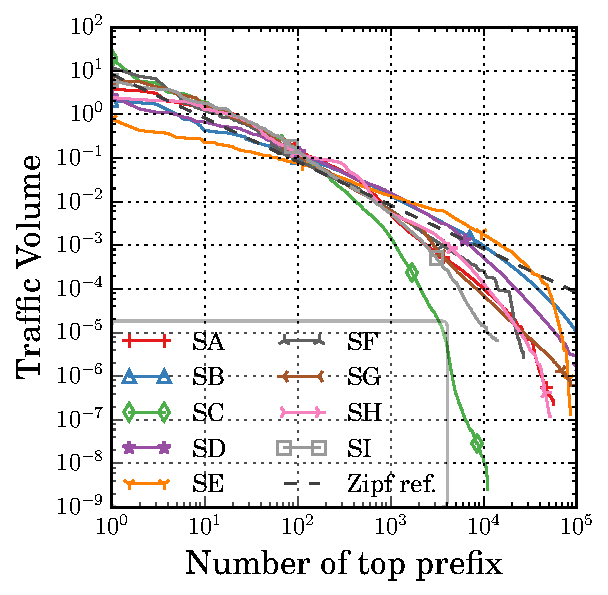
\includegraphics[width=\textwidth]{gfx/chap2/loglog_multi_site.pdf}
                \caption{Week volume share, log-log.}
                \label{fig:week_zipf}
        \end{subfigure}  
        \hfill
        \begin{subfigure}[b]{0.49\textwidth}
        		\centering
                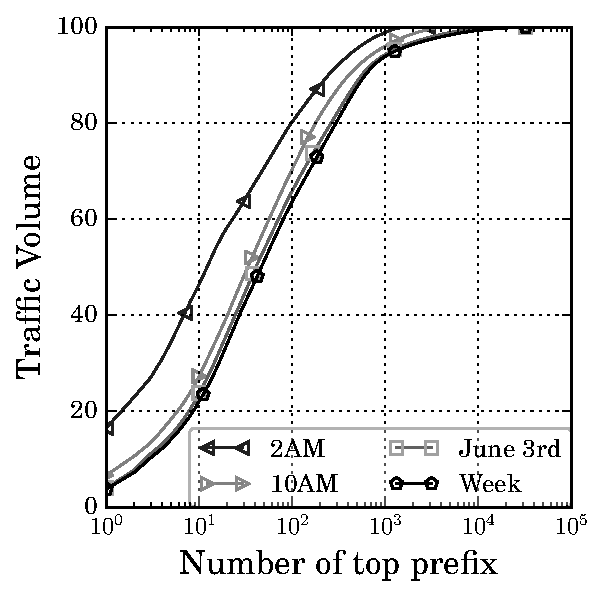
\includegraphics[width=\textwidth]{gfx/chap2/cdf_multi_time.pdf}
                \caption{CDF, different time spans, SA.}
                \label{fig:sa_cdf_multi_time}
        \end{subfigure}    
\caption{Traffic distribution among BGP prefixes.}\label{fig:traffic_dis_site}
\end{figure}

As outlined earlier, the feasibility of prefix selection is based on the assumption that most traffic  concentrates on a few popular destinations.
Some previous works have shown this property with their own datasets~\cite{Fang1999,Feamster2003, Wallerich2006}. 
We demonstrate here that our dataset as well has this phenomenon of uneven traffic distribution across destination prefixes.

In Figure~\ref{fig:week_zipf}, the volume share (percentage in unit, on the y-axis) of each BGP prefix is plotted for the week starting from June 1st, 2015.
Prefixes are decreasingly sorted along the X-axis according to their cumulative volume fraction over the week.
The X-axis labels indicate rankings of prefixes.
We observe that the week volume associated with BGP prefixes can be approximately described by a reference Zipf's distribution with $N=10^5, s=1$ (dashed line).\footnote{Zipf's law defines that the $k^{th}$ most popular element among total $N$ elements has an occurrence share of $f(k,s,N)=\frac{1/k^s}{\sum_{n=1}^{N}1/n^s}$.} 
This figure shows that Internet traffic (within our dataset) is indeed highly concentrated on a few prefixes.



Figure~\ref{fig:sa_cdf_multi_time} compares the traffic distribution (in CDF) of SA at different time resolutions: prefix volumes within one hour time (at 2AM and 10AM), traffic accumulated over 24 hours (on June 3rd) and that throughout the full week.
The uneven traffic distribution is not unique on week time scales (Figure~\ref{fig:week_zipf}), but as well demonstrates over shorter time ranges.
Moreover, the level of traffic concentration over BGP prefixes actually varies within in a day.
The $1^{st}$ ranking prefix at 2AM represents almost $20\%$ of all traffic, while at other time or time spans, this ratio is much lower. This observation leads to the study in the following section.
This change in time leads to the study in the following section.

\subsection{Temporal dynamism of traffic over BGP prefixes}
\label{sec:dyna}
We are interested in understanding how traffic volume evolves over time, and how this dynamism is reflected in uneven traffic distribution.

\subsubsection{Coefficient of Variation}
In this section we mainly use Coefficient of Variation ($c_v$) to characterize the traffic volume volatility over time for each BGP prefix.
The study uses the data over one entire week starting from June 1st, 2015.
In order to facilitate the discussion, we first introduce some notations.

Each destination prefix $P$ ever active during a week is associated with a volume time series $v(P)={\left\{ v(P)_h\right\} }_{h=1, \dots, 168}$ that
stores its traffic volume over the week at hour interval. 
We calculate the Coefficient of Variation ($c_v$) for prefix $P$ according to
\begin{equation*}
c_v(P) = \frac{\delta(v(P))}{\mu(v(P))},
\label{eq:cv}
\end{equation*}
where $\delta$ stands for the calculation of standard deviation and $\mu$ for mean.

$c_v$ can be regarded as a measure of traffic volume variation in relation to its hourly mean over a week.
A larger $c_v(P)$ value suggests that the $v(P)$ tend to take values in a bigger range that is normalized by its average level. 
Consequently it becomes more difficult to anticipate the traffic volumes for this prefix $P$~\cite{He2005}.\footnote{By construction, the maximum $c_v$ for a hourly volume series of 168 in length is $\sqrt{167}$, corresponding to the case where the prefix in question is active during only one single hour throughout the entire week.}

\begin{figure}[!htb]
\centering
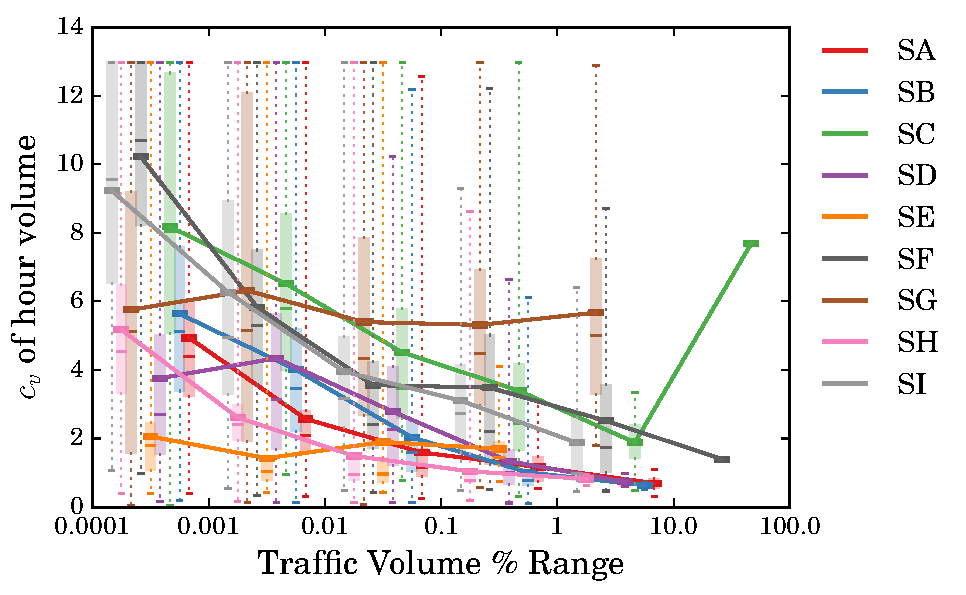
\includegraphics[width=1\textwidth]{gfx/chap2/cv_bin.pdf}
\caption{Relation between $\{c_v(P)\}_P$  and  week volume share for all BGP prefixes $P$. 
}
\label{fig:cv}
\end{figure}

Further, we are interested in knowing how the $c_v$ value is related to prefixes of different volume importance. For example, are prefix with big volumes tend to be more stable or volatile over time?
To answer such question, we visualize the relationship between $c_v$ and prefix volume in Figure~\ref{fig:cv}.
Each prefix is sorted along the X-axis according to its accumulated volume share over the week.
Prefixes with large volume share are located on the right side.
To compact the visual representation, we further group all the prefix into six bins, representing different discrete level of volume importance.
These bins can be identified with the X-axis labels.
They are $[10^{-4}, 10^{-3})$, $[10^{-3}, 10^{-2})$, all the way to $[10,100)$.
For all the prefixes within in same bin, we summarize their $c_v$ using a vertical boxplot.
The two ends of the box represent $25^th$ and $75^th$ percentile $c_v$ values of prefixes within the bin.
The thin line in the middle stands for median, while the thick one for mean.
The whiskers are min and max separately.
In order to outline the relationship between $c_v$ and prefix volume importance, the mean value of the six bins are connected with a thick line.

From this Figure, we observe that for all the networks except SG and SE, $c_v$ of large volume prefixes tends to be smaller in average and constrained in a narrower box. 
On the contrary, the prefixes with smaller week volume share tend to have larger $c_v$ values.
It allows us to capture a significant part of the overall traffic (represented by those stable and large prefixes) by simply picking the prefixes with large average hour volume. 

\subsubsection{\textit{Core} presence intensity}
We continue to explore traffic dynamism from another perspective:
for each hour $h$, we define the $core_h$ as the set containing top ranking prefixes that represent $95\%$ of total traffic. 
Imagine that we were to identify prefixes representing that much traffic, then $core_h$ will be the smallest set that we could arrive at.
One essential feature of the \textit{core} set is its size.
It gives a rough picture on how many prefixes that a network might want to consider in measurement-based TE.
Table~\ref{tab:core_size} lists 1) the average number of prefixes included in the \textit{core} (\textit{core} size can change over time), 2) the average \textit{core} size percentage with regard to the average number of active prefixes each hour and 3) the maximum size of the \textit{core} set over the week.
For a big part of the networks in our dataset, \textit{core} set only represents a small fraction of active prefixes.
This observation is in line with the uneven traffic distribution demonstrated earlier.

\begin{table}[!htb]
\centering
\footnotesize
\begin{tabular}{cccc}\toprule
\textbf{Name} & \textbf{Avg. prefix \#} & \textbf{$\%$ w.r.t active prefix} & \textbf{Max prefix \#}\\
\midrule
SA & 629  & 17.87  & 1051\\
SB & 5264 & 9.45  & 13934\\
SC & 73  & 4.59    & 177\\
SD & 2481  & 17.35 & 3757\\
SE & 15501  & 53.61 & 20900\\
SF & 377  & 30.73    & 772\\
SG & 570 & 7.76    & 1766\\
SH & 965  & 19.42   & 1731\\
SI & 175  & 21.00    & 415\\
\bottomrule
\end{tabular}
\caption{Core prefix set statistics.}
\label{tab:core_size}
\end{table}

If a prefix is inside the \textit{core} at a certain hour, it can be regarded important for bringing a significant amount of traffic.
We thus define the ``\textit{core} presence'' for a prefix $P$ at each hour $h$ as:
\begin{equation*}
cp(P)_i = \begin{dcases*}
        1  & when $P \in$ $\textit{core}_i$,\\
        0 & otherwise,
        \end{dcases*}
\label{eq:cp}
\end{equation*}
% $cp(P)$ is a time series with which we can further describe the frequency or likelihood of prefix being present in the \textit{core} over the week: 
The \textit{core} presence intensity $I_{cp}(P)$ is then defined as the frequency of \textit{core} presence over the week:
$I_{cp}(P, 168) = \frac{1}{168} \sum_{i=1}^{168} cp(P)_i$.
Intuitively, $I_{cp}$ can be regarded as an indicator of fitness that a prefix shall be continuously monitored in measurement-based TE.
Again, we are interested in knowing how the value of $I_{cp}$ relates to the overall traffic volume importance.
Similarly, we visualized this relationship in Figure~\ref{fig:cpi}, using the same visual language employed in Figure~\ref{fig:cv}.

\begin{figure}[!tb]
\centering
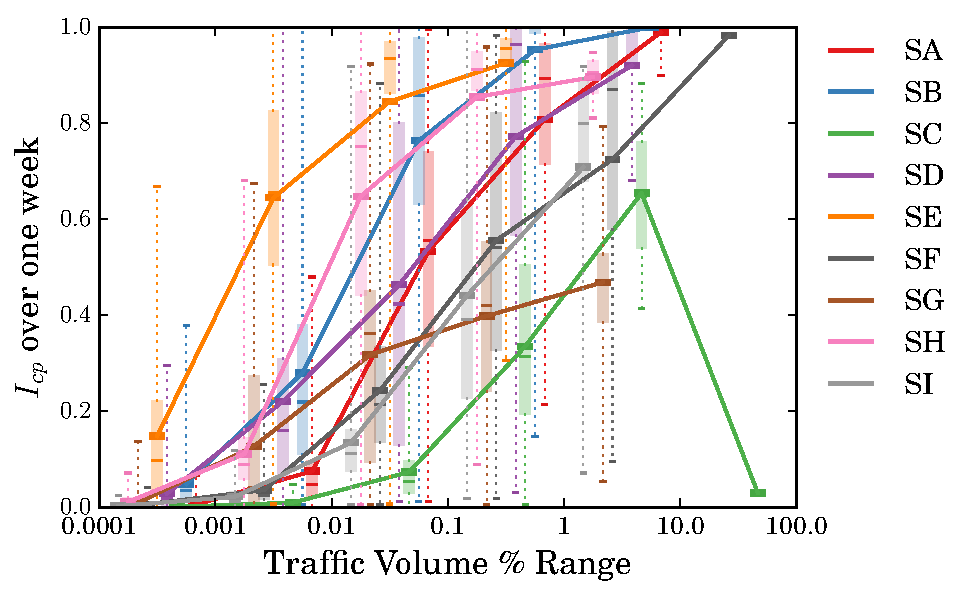
\includegraphics[width=1\textwidth]{gfx/chap2/cp_bin.pdf}
\caption{Relation between $I_{cp}$ over the week and week volume fraction of BGP prefixes.}
\label{fig:cpi}
\end{figure}

For all the networks, we can see that prefixes with bigger week volume share are more likely to have a high $I_{cp}$ over the week, i.e. they appear frequently in the \textit{core}.
We can conclude that by focusing on prefixes that intensively appear in the \textit{core} throughout the week, we will be able to capture a large part of the prefixes associated with important traffic volume over the week.

\subsubsection{Relationship between $I_{cp}$ and $c_v$}
\begin{figure}
		\centering
        \begin{subfigure}[b]{0.49\textwidth}
                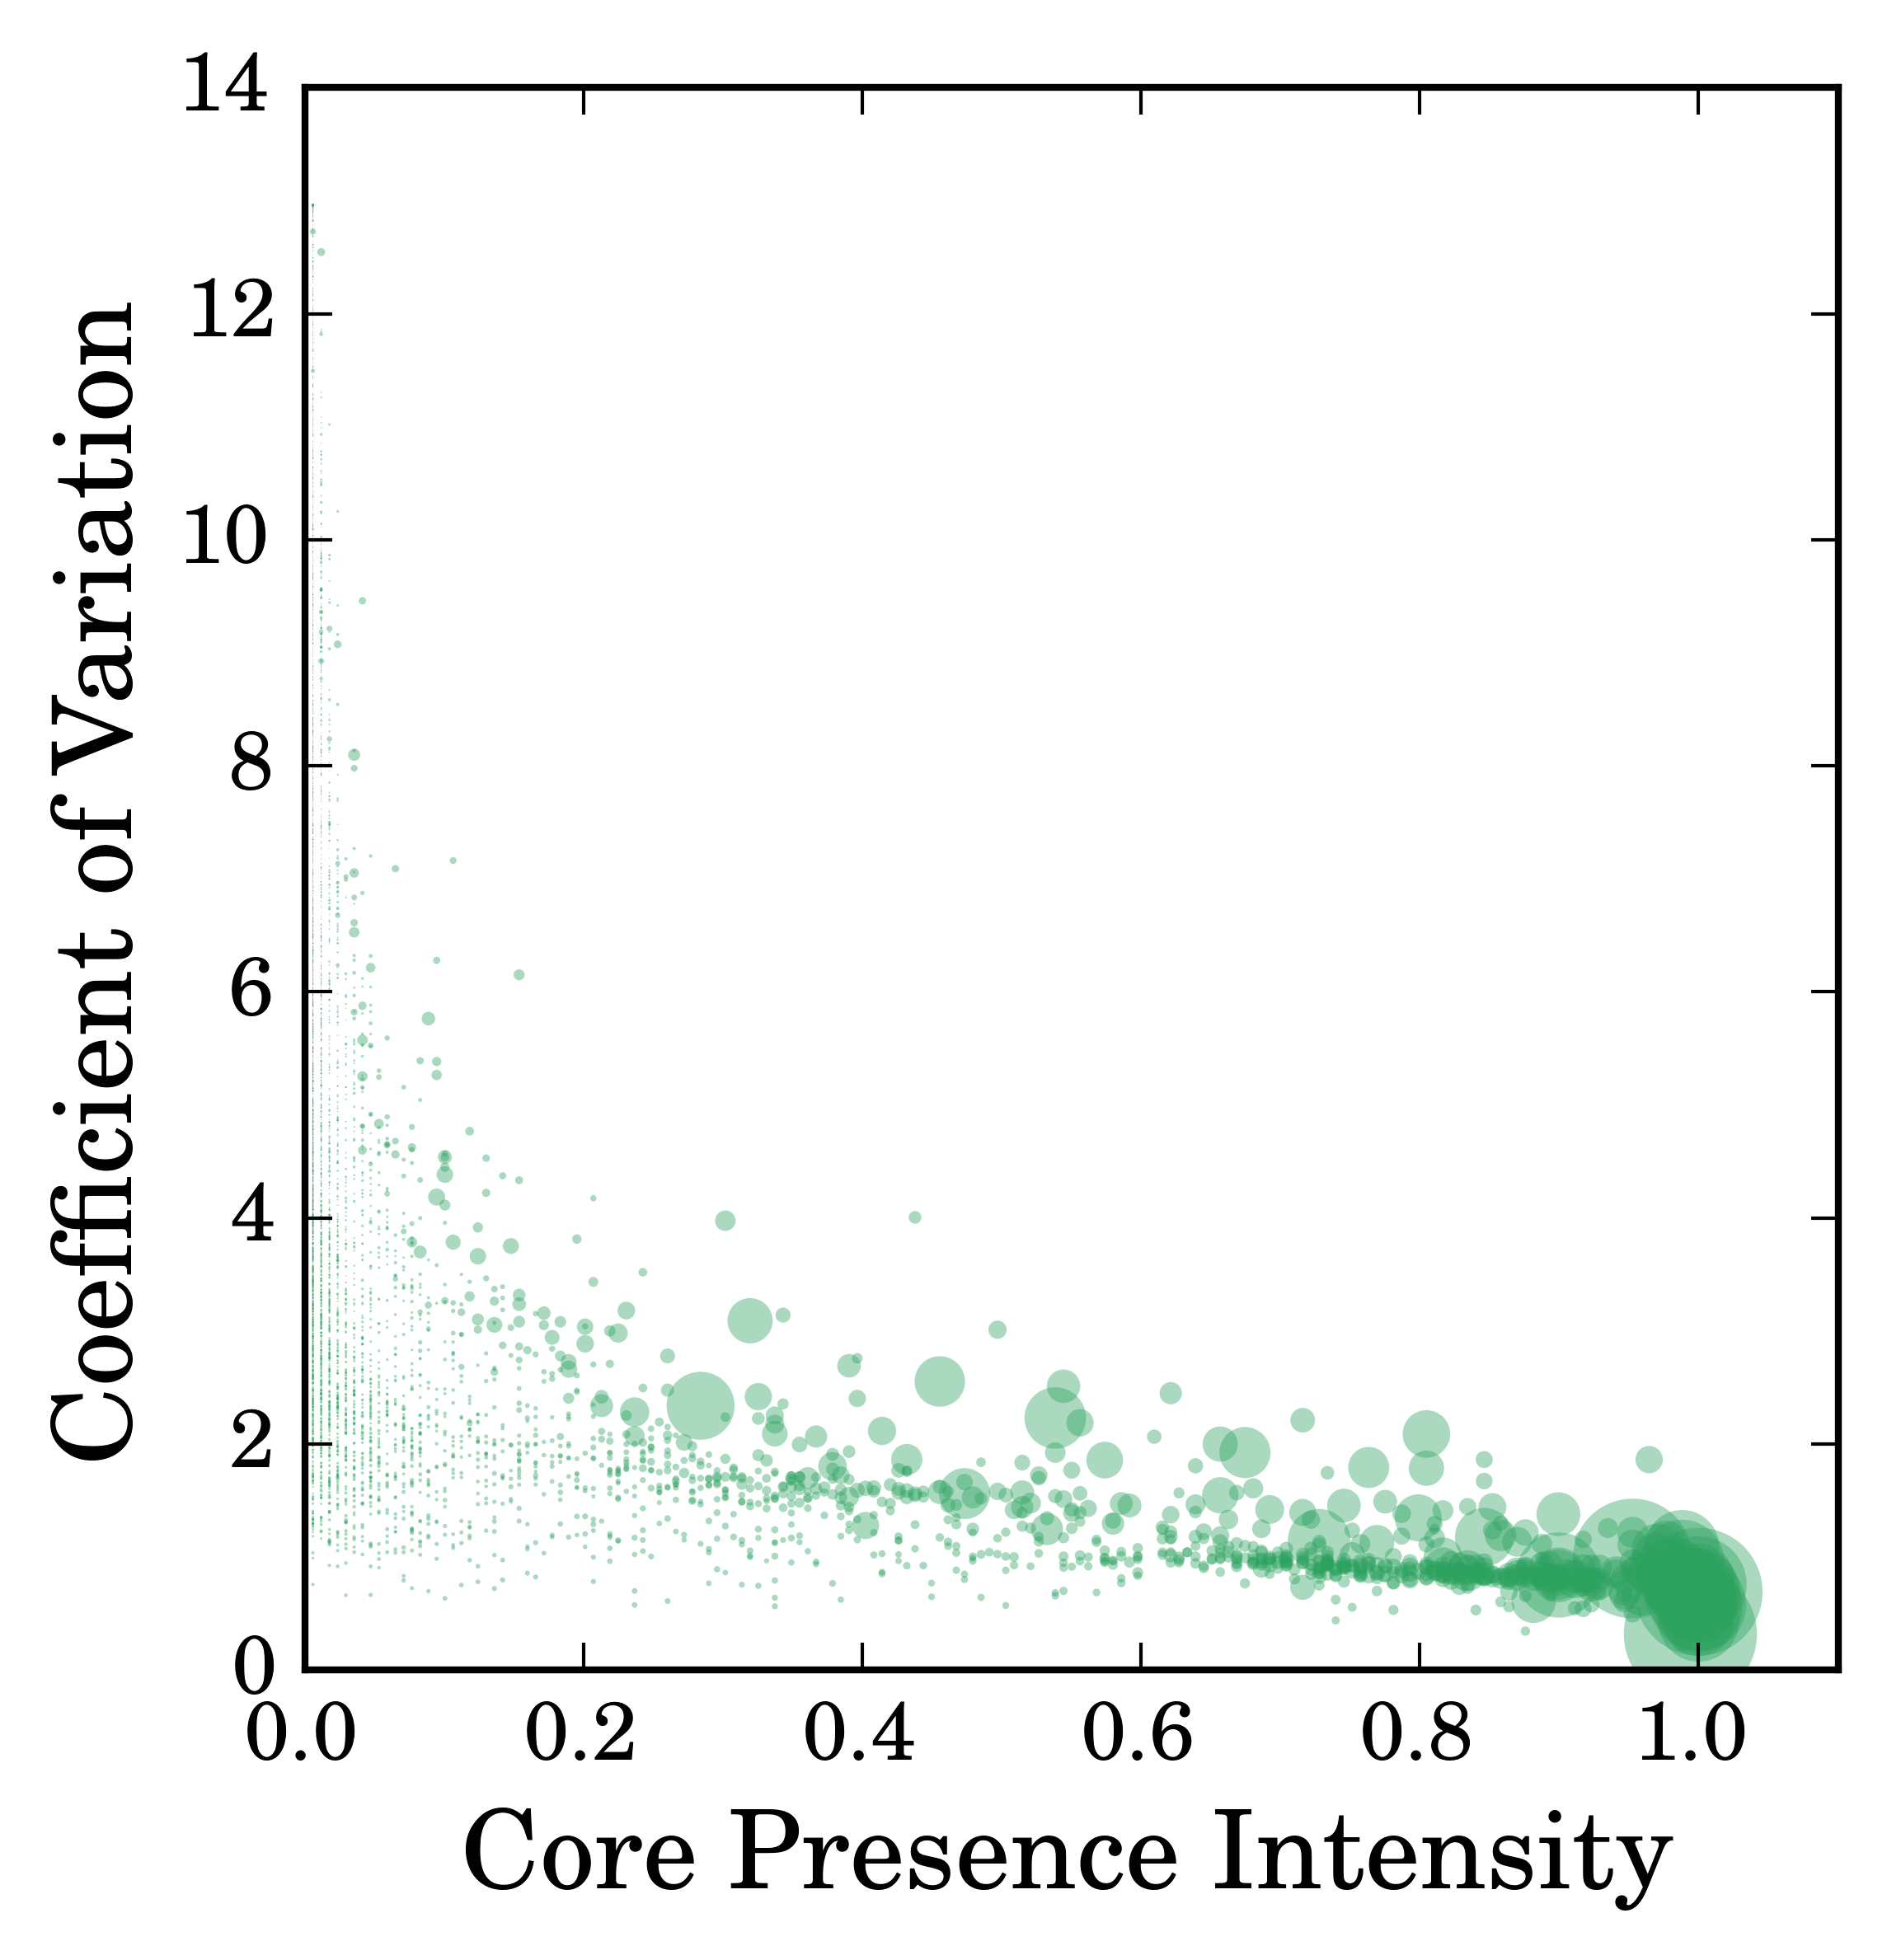
\includegraphics[width=\textwidth]{gfx/chap2/corre_cv_cp_sa.png}
                \caption{SA, 56684 prefixes}
                \label{fig:cv_cp_sa}
        \end{subfigure}
        \begin{subfigure}[b]{0.49\textwidth}
                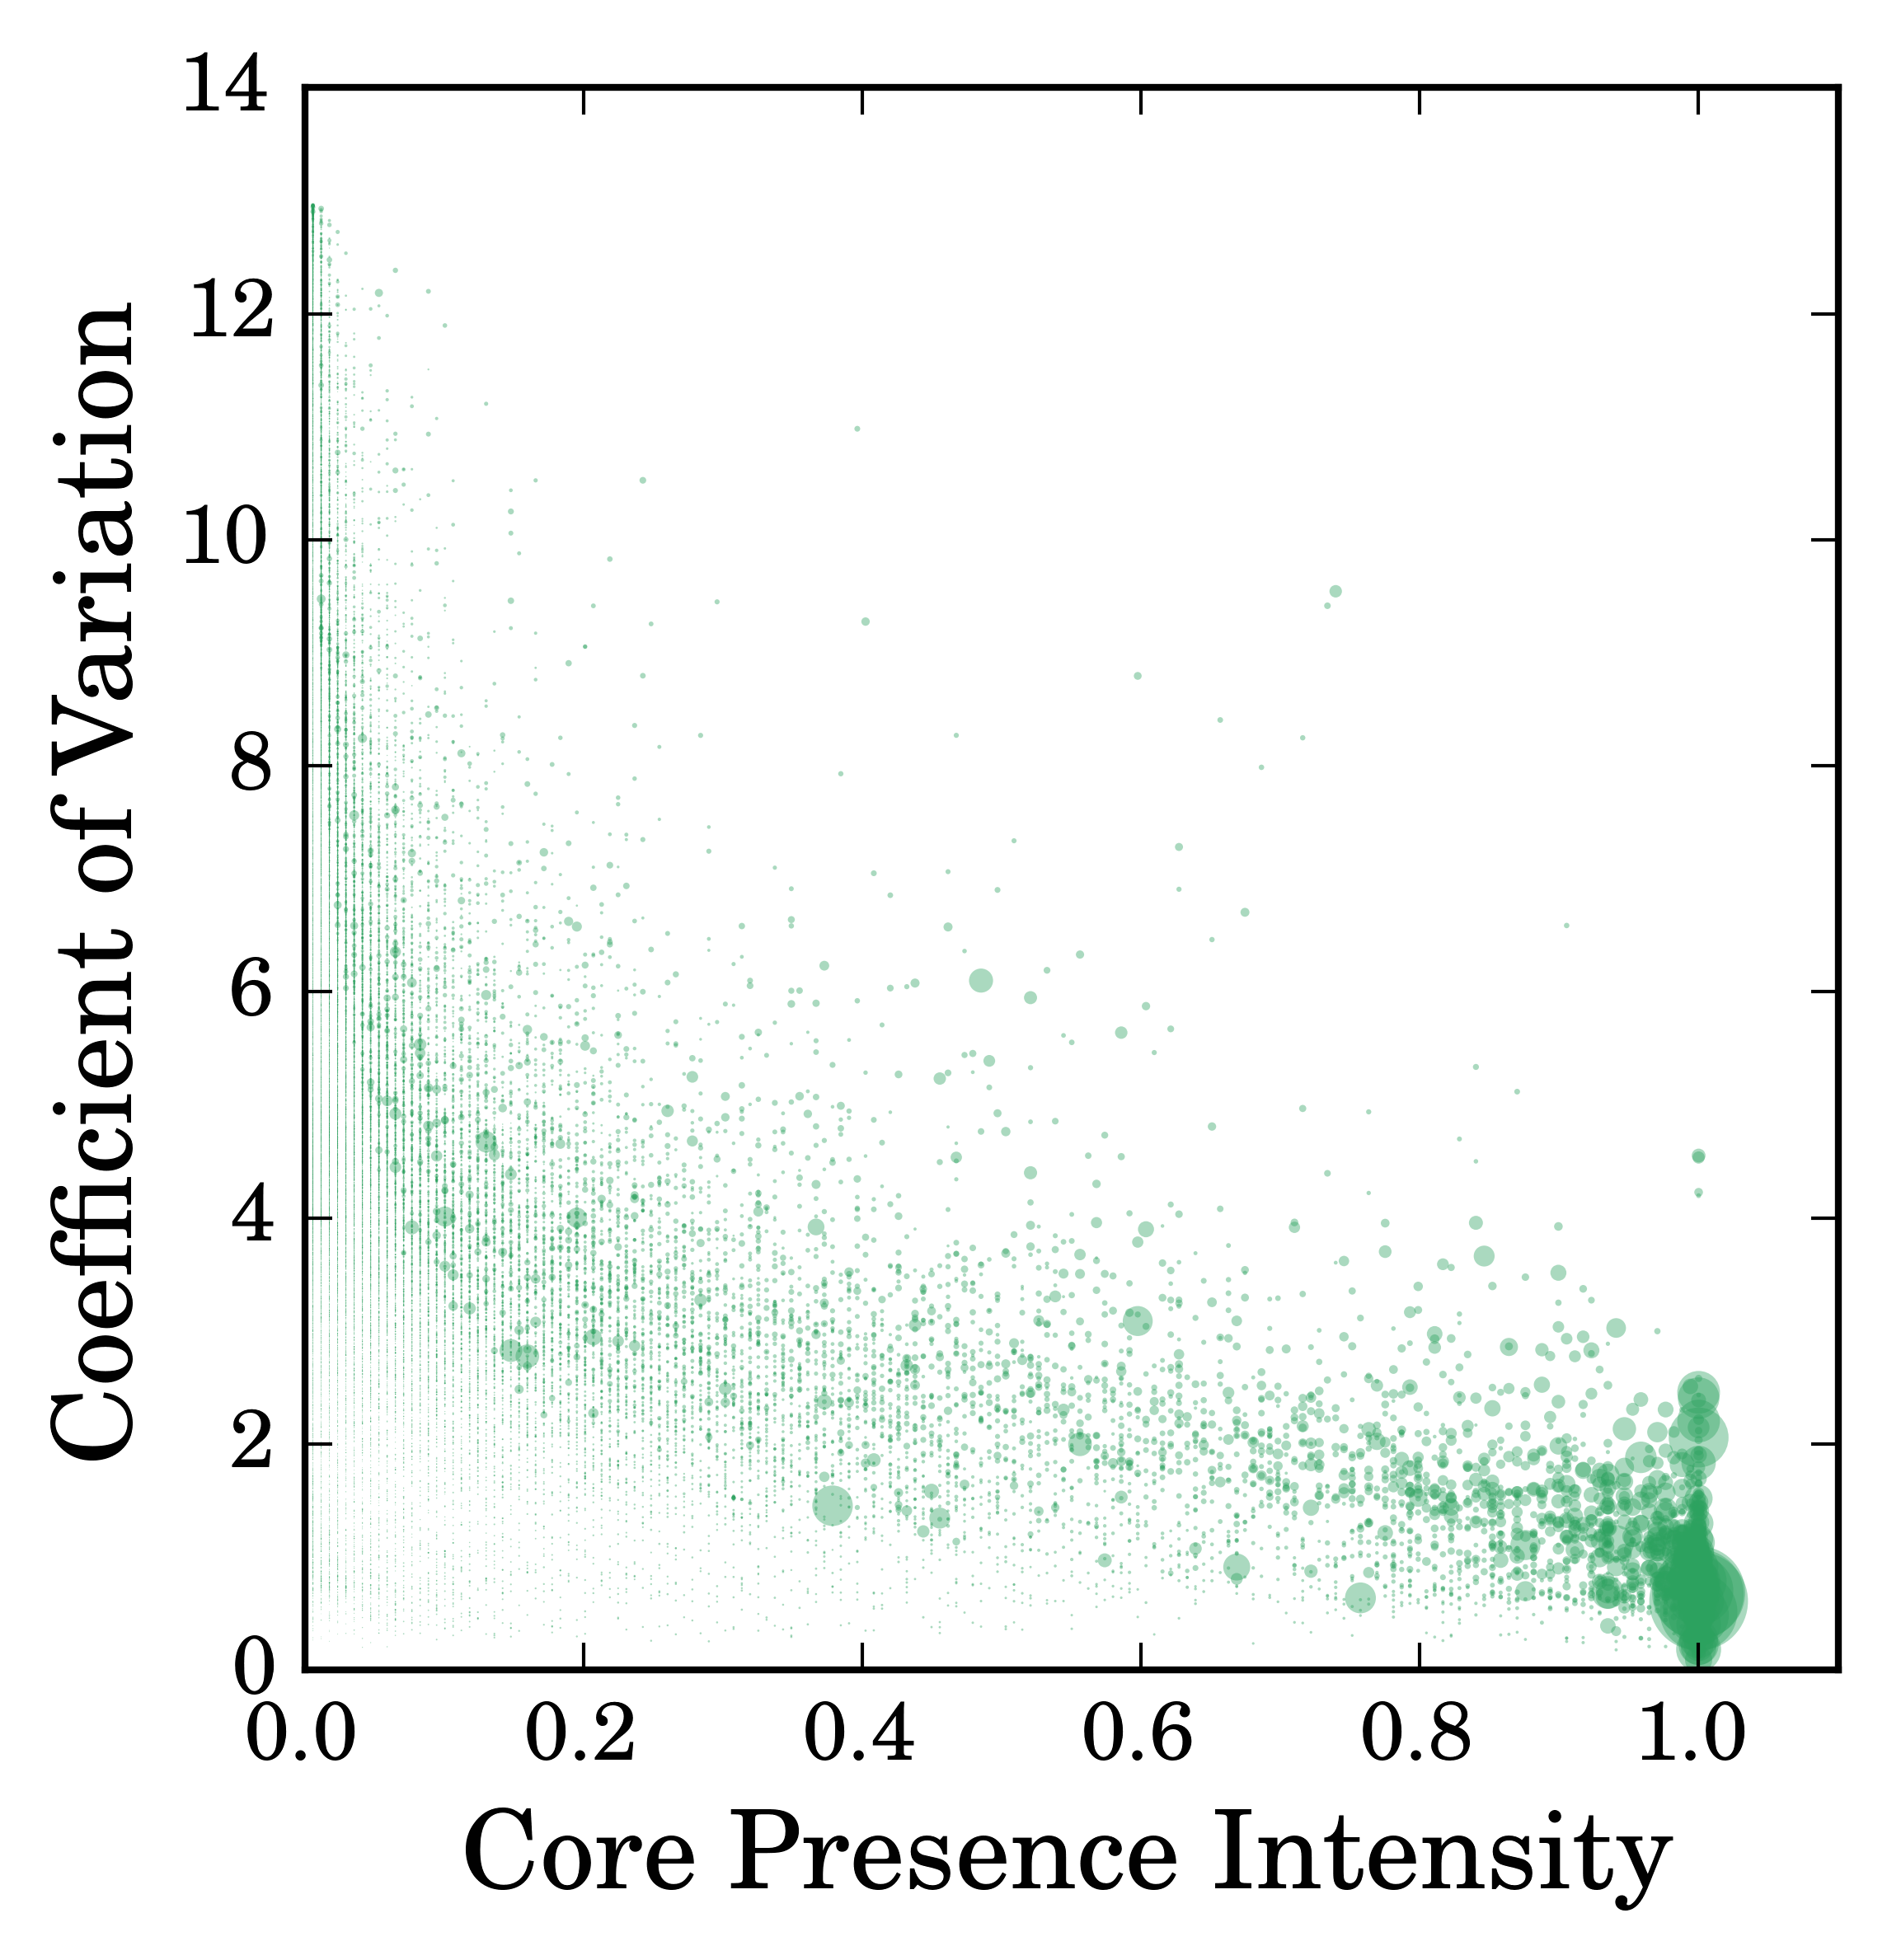
\includegraphics[width=\textwidth]{gfx/chap2/corre_cv_cp_sb.png}
                \caption{SB, 504707 prefixes}
                \label{fig:cv_cp_sb}
        \end{subfigure}
        \begin{subfigure}[b]{0.49\textwidth}
                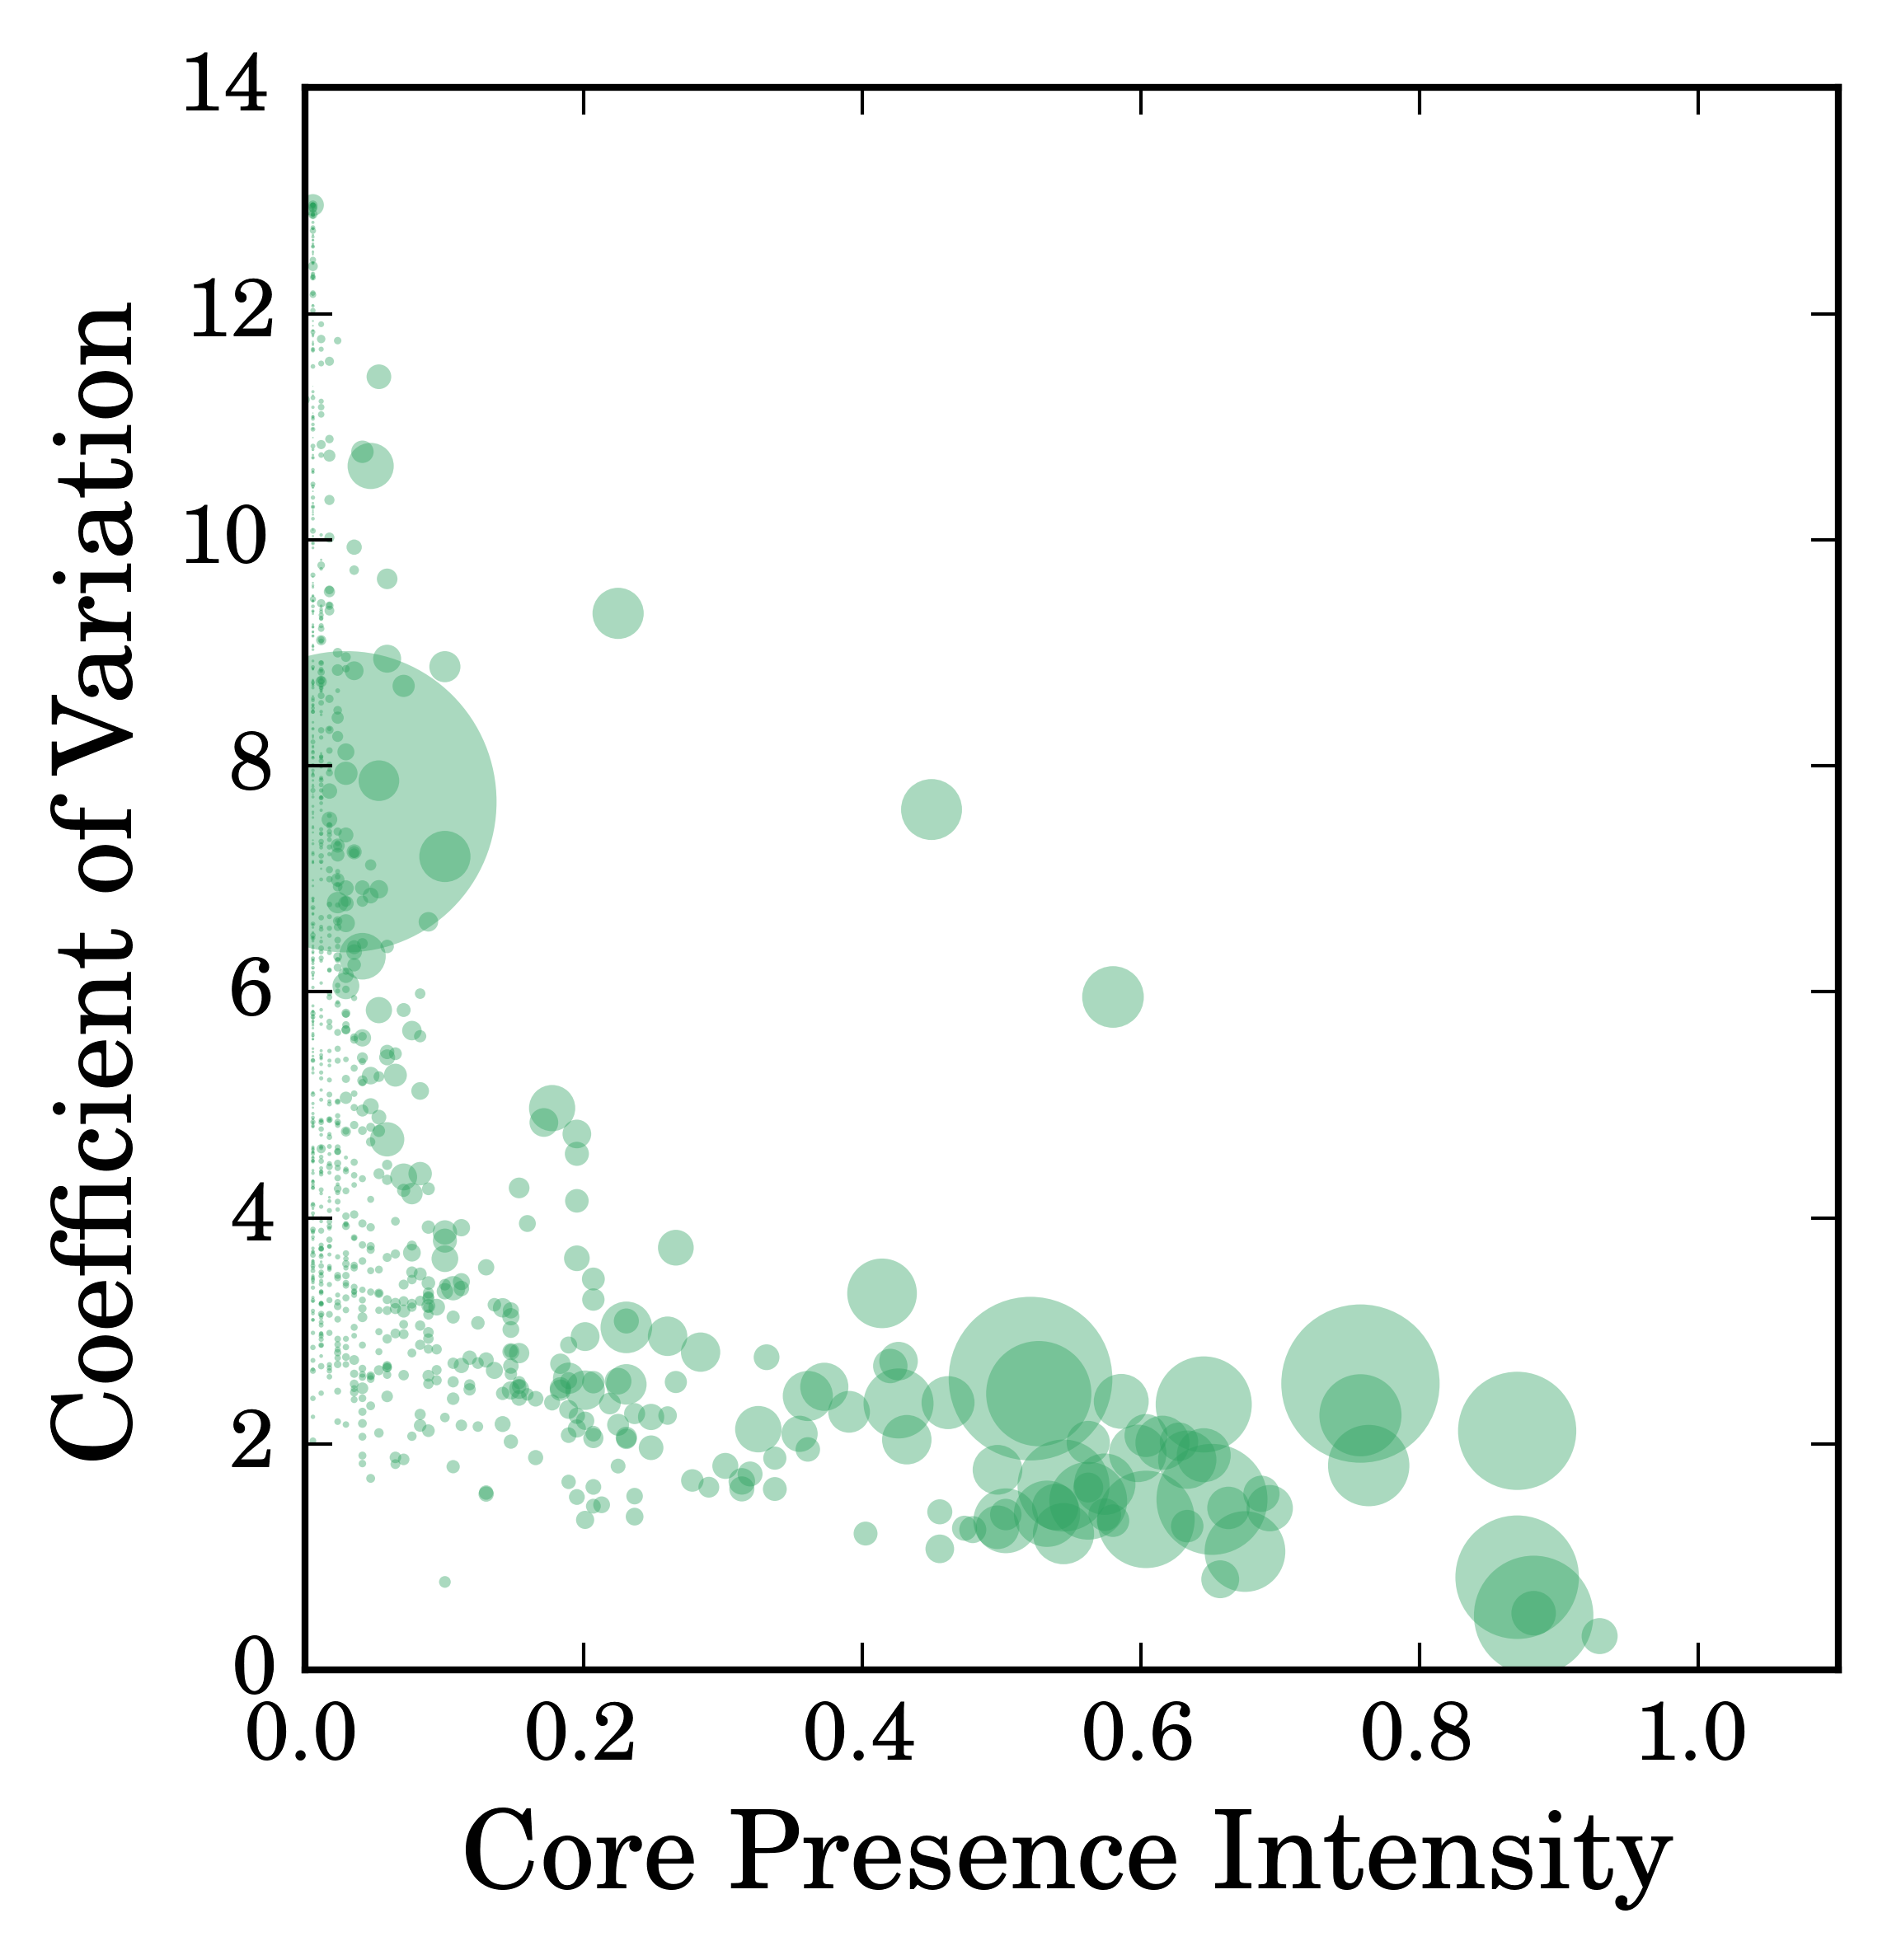
\includegraphics[width=\textwidth]{gfx/chap2/corre_cv_cp_sc.png}
                \caption{SC, 11065 prefixes}
                \label{fig:cv_cp_sc}
        \end{subfigure}
        \begin{subfigure}[b]{0.49\textwidth}
                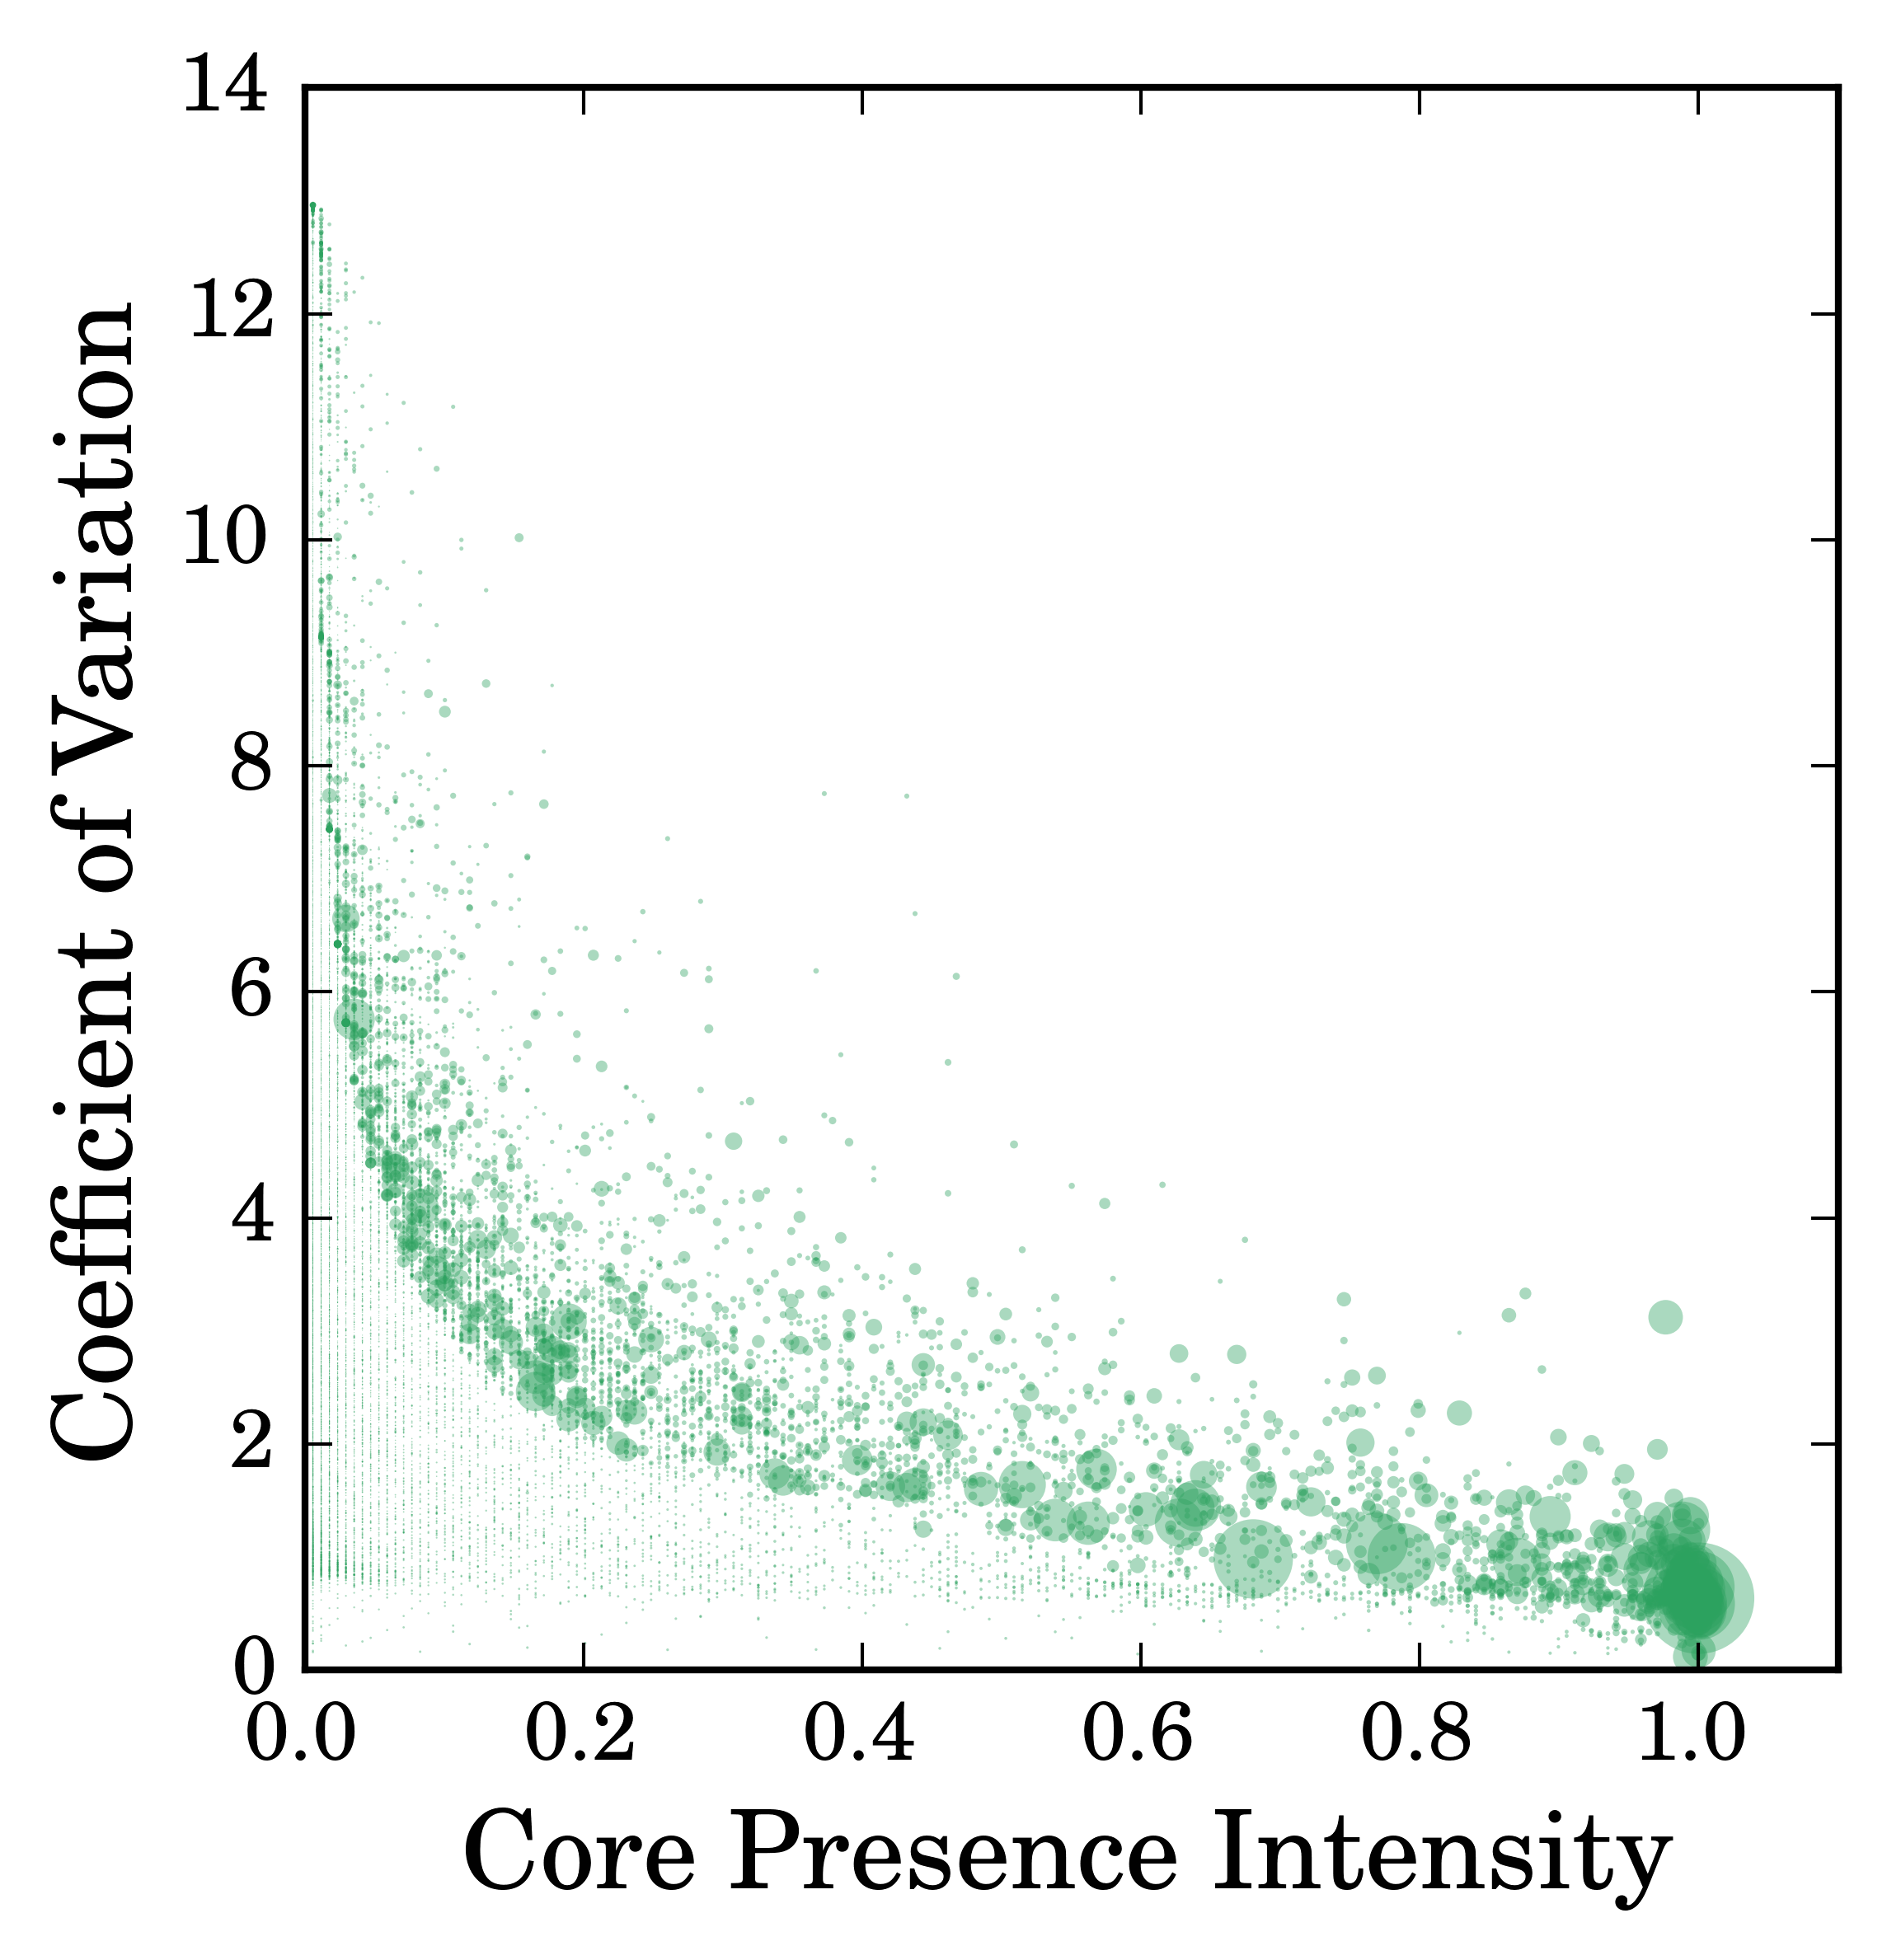
\includegraphics[width=\textwidth]{gfx/chap2/corre_cv_cp_sd.png}
                \caption{SD, 140700 prefixes}
                \label{fig:cv_cp_sd}
        \end{subfigure}
        \begin{subfigure}[b]{0.49\textwidth}
                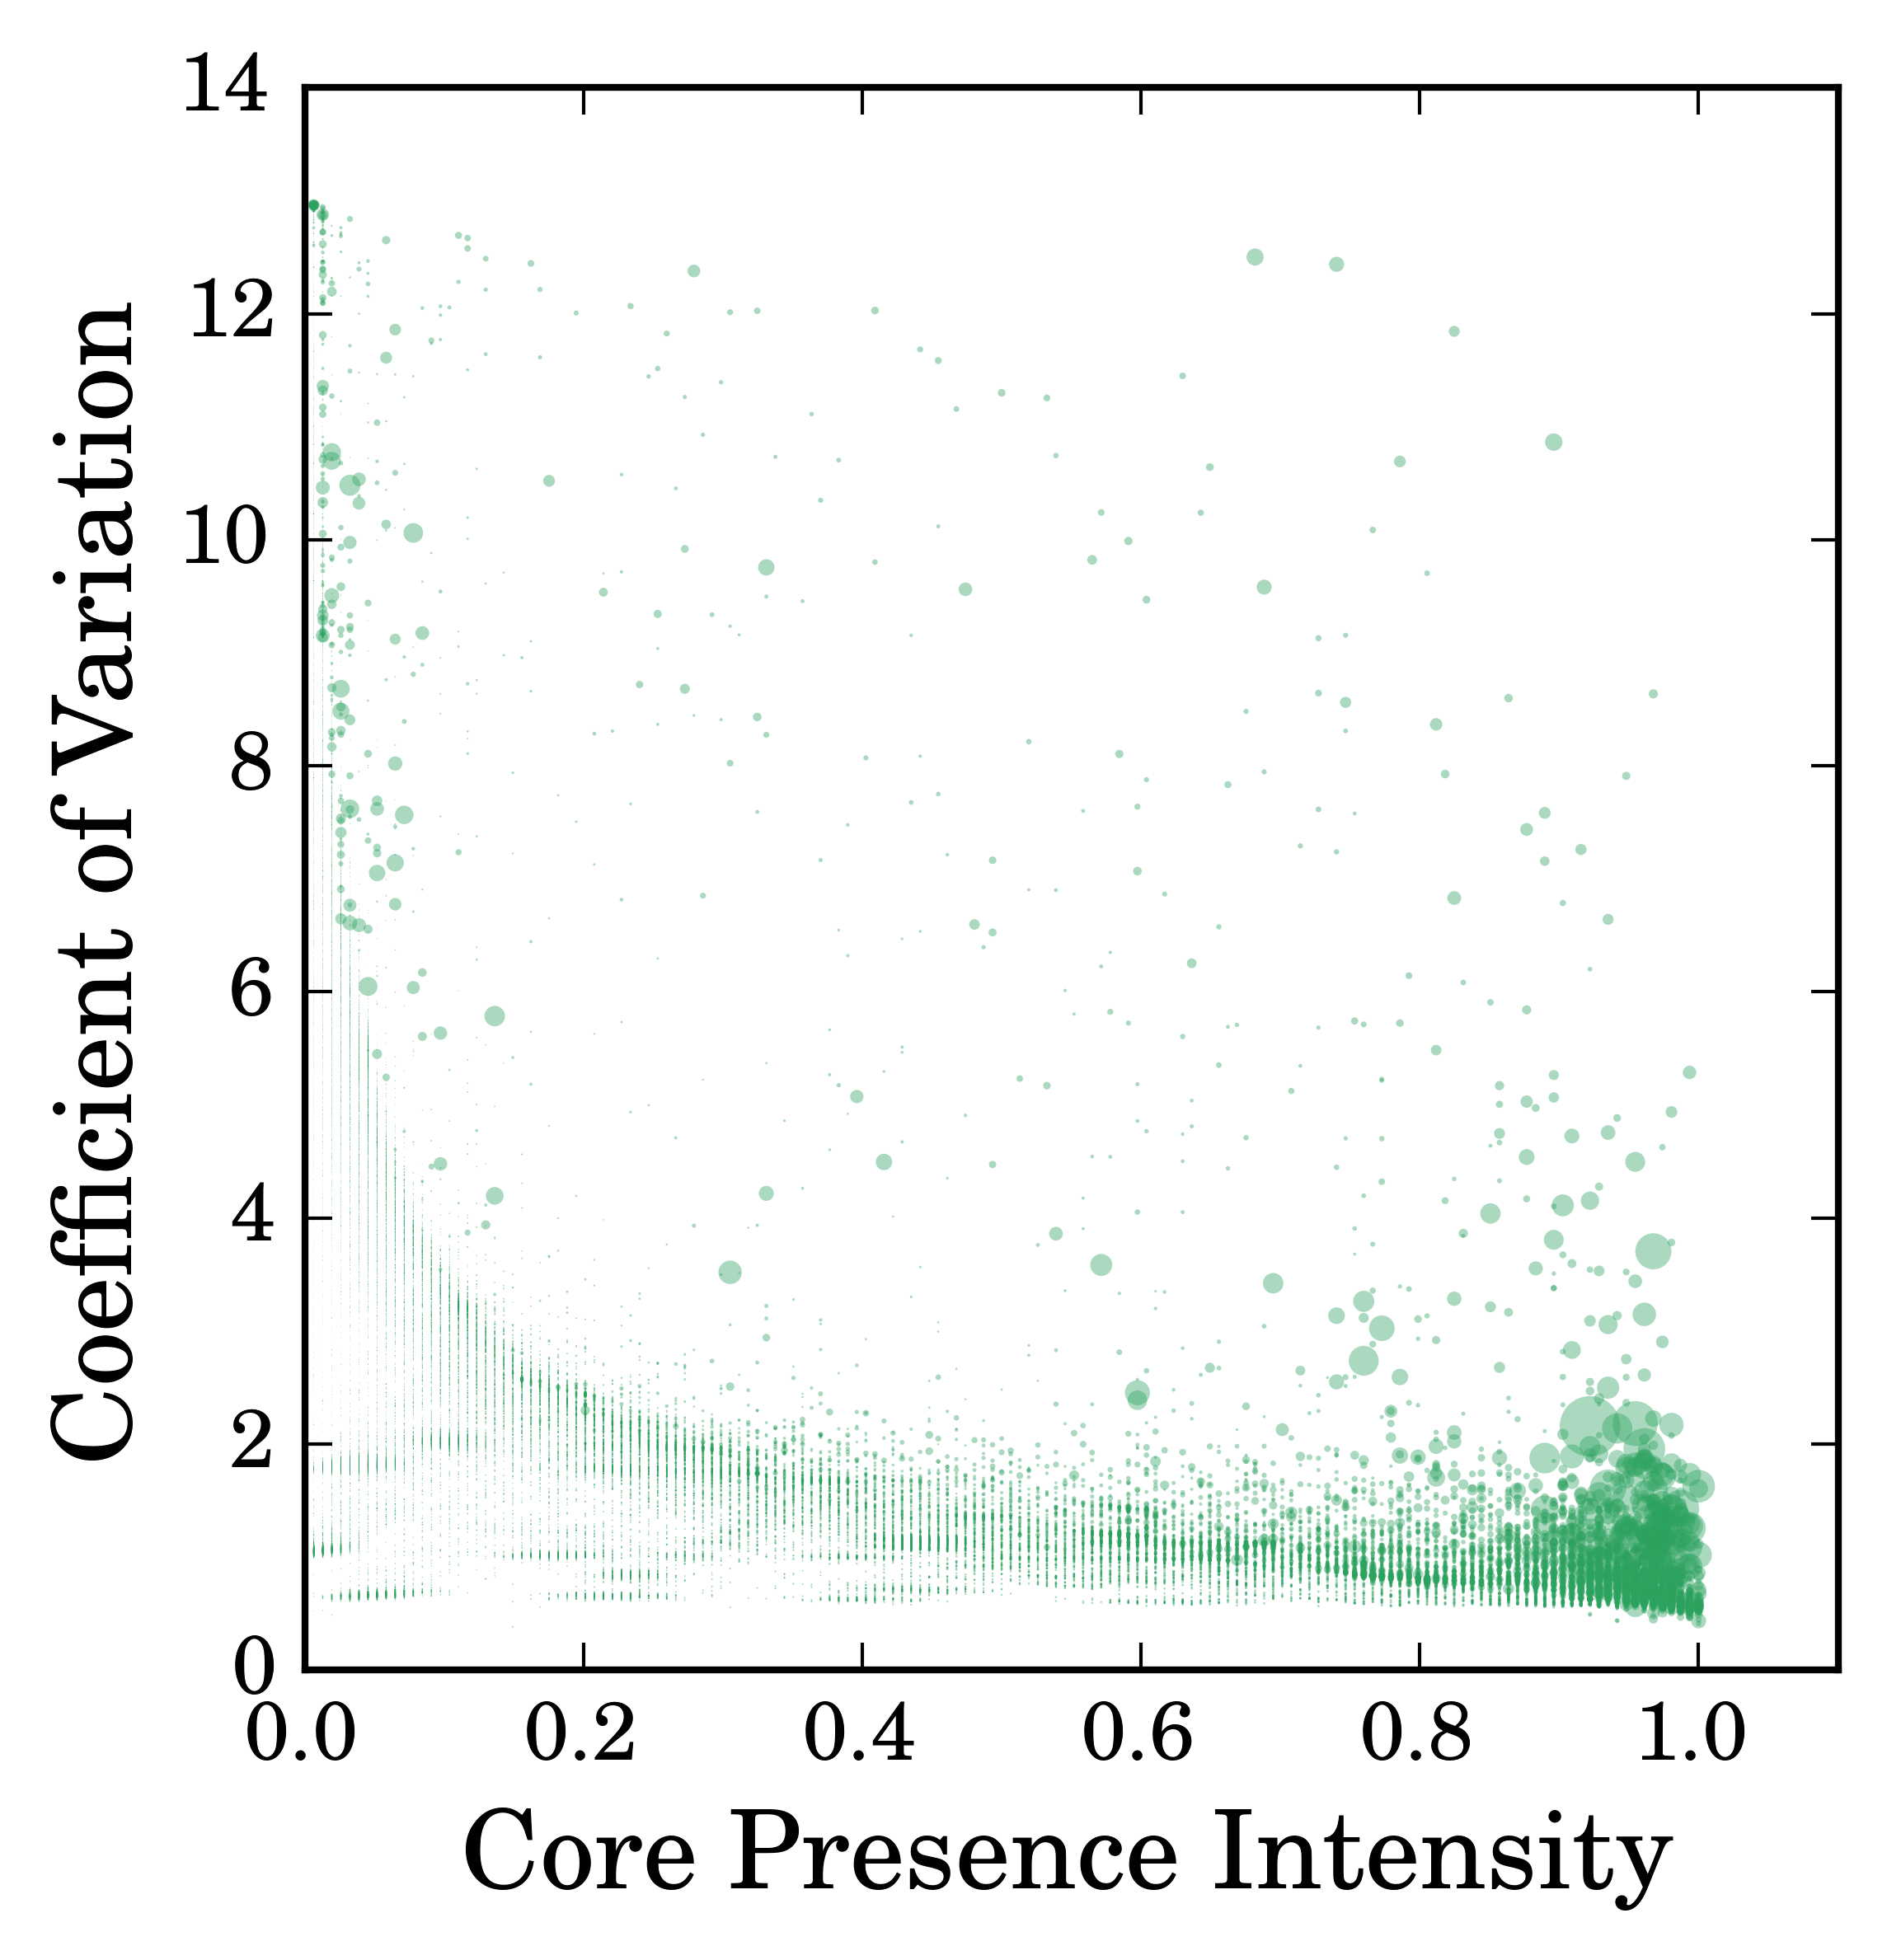
\includegraphics[width=\textwidth]{gfx/chap2/corre_cv_cp_se.png}
                \caption{SE, 86014 prefixes}
                \label{fig:cv_cp_se}
        \end{subfigure}
        \begin{subfigure}[b]{0.49\textwidth}
                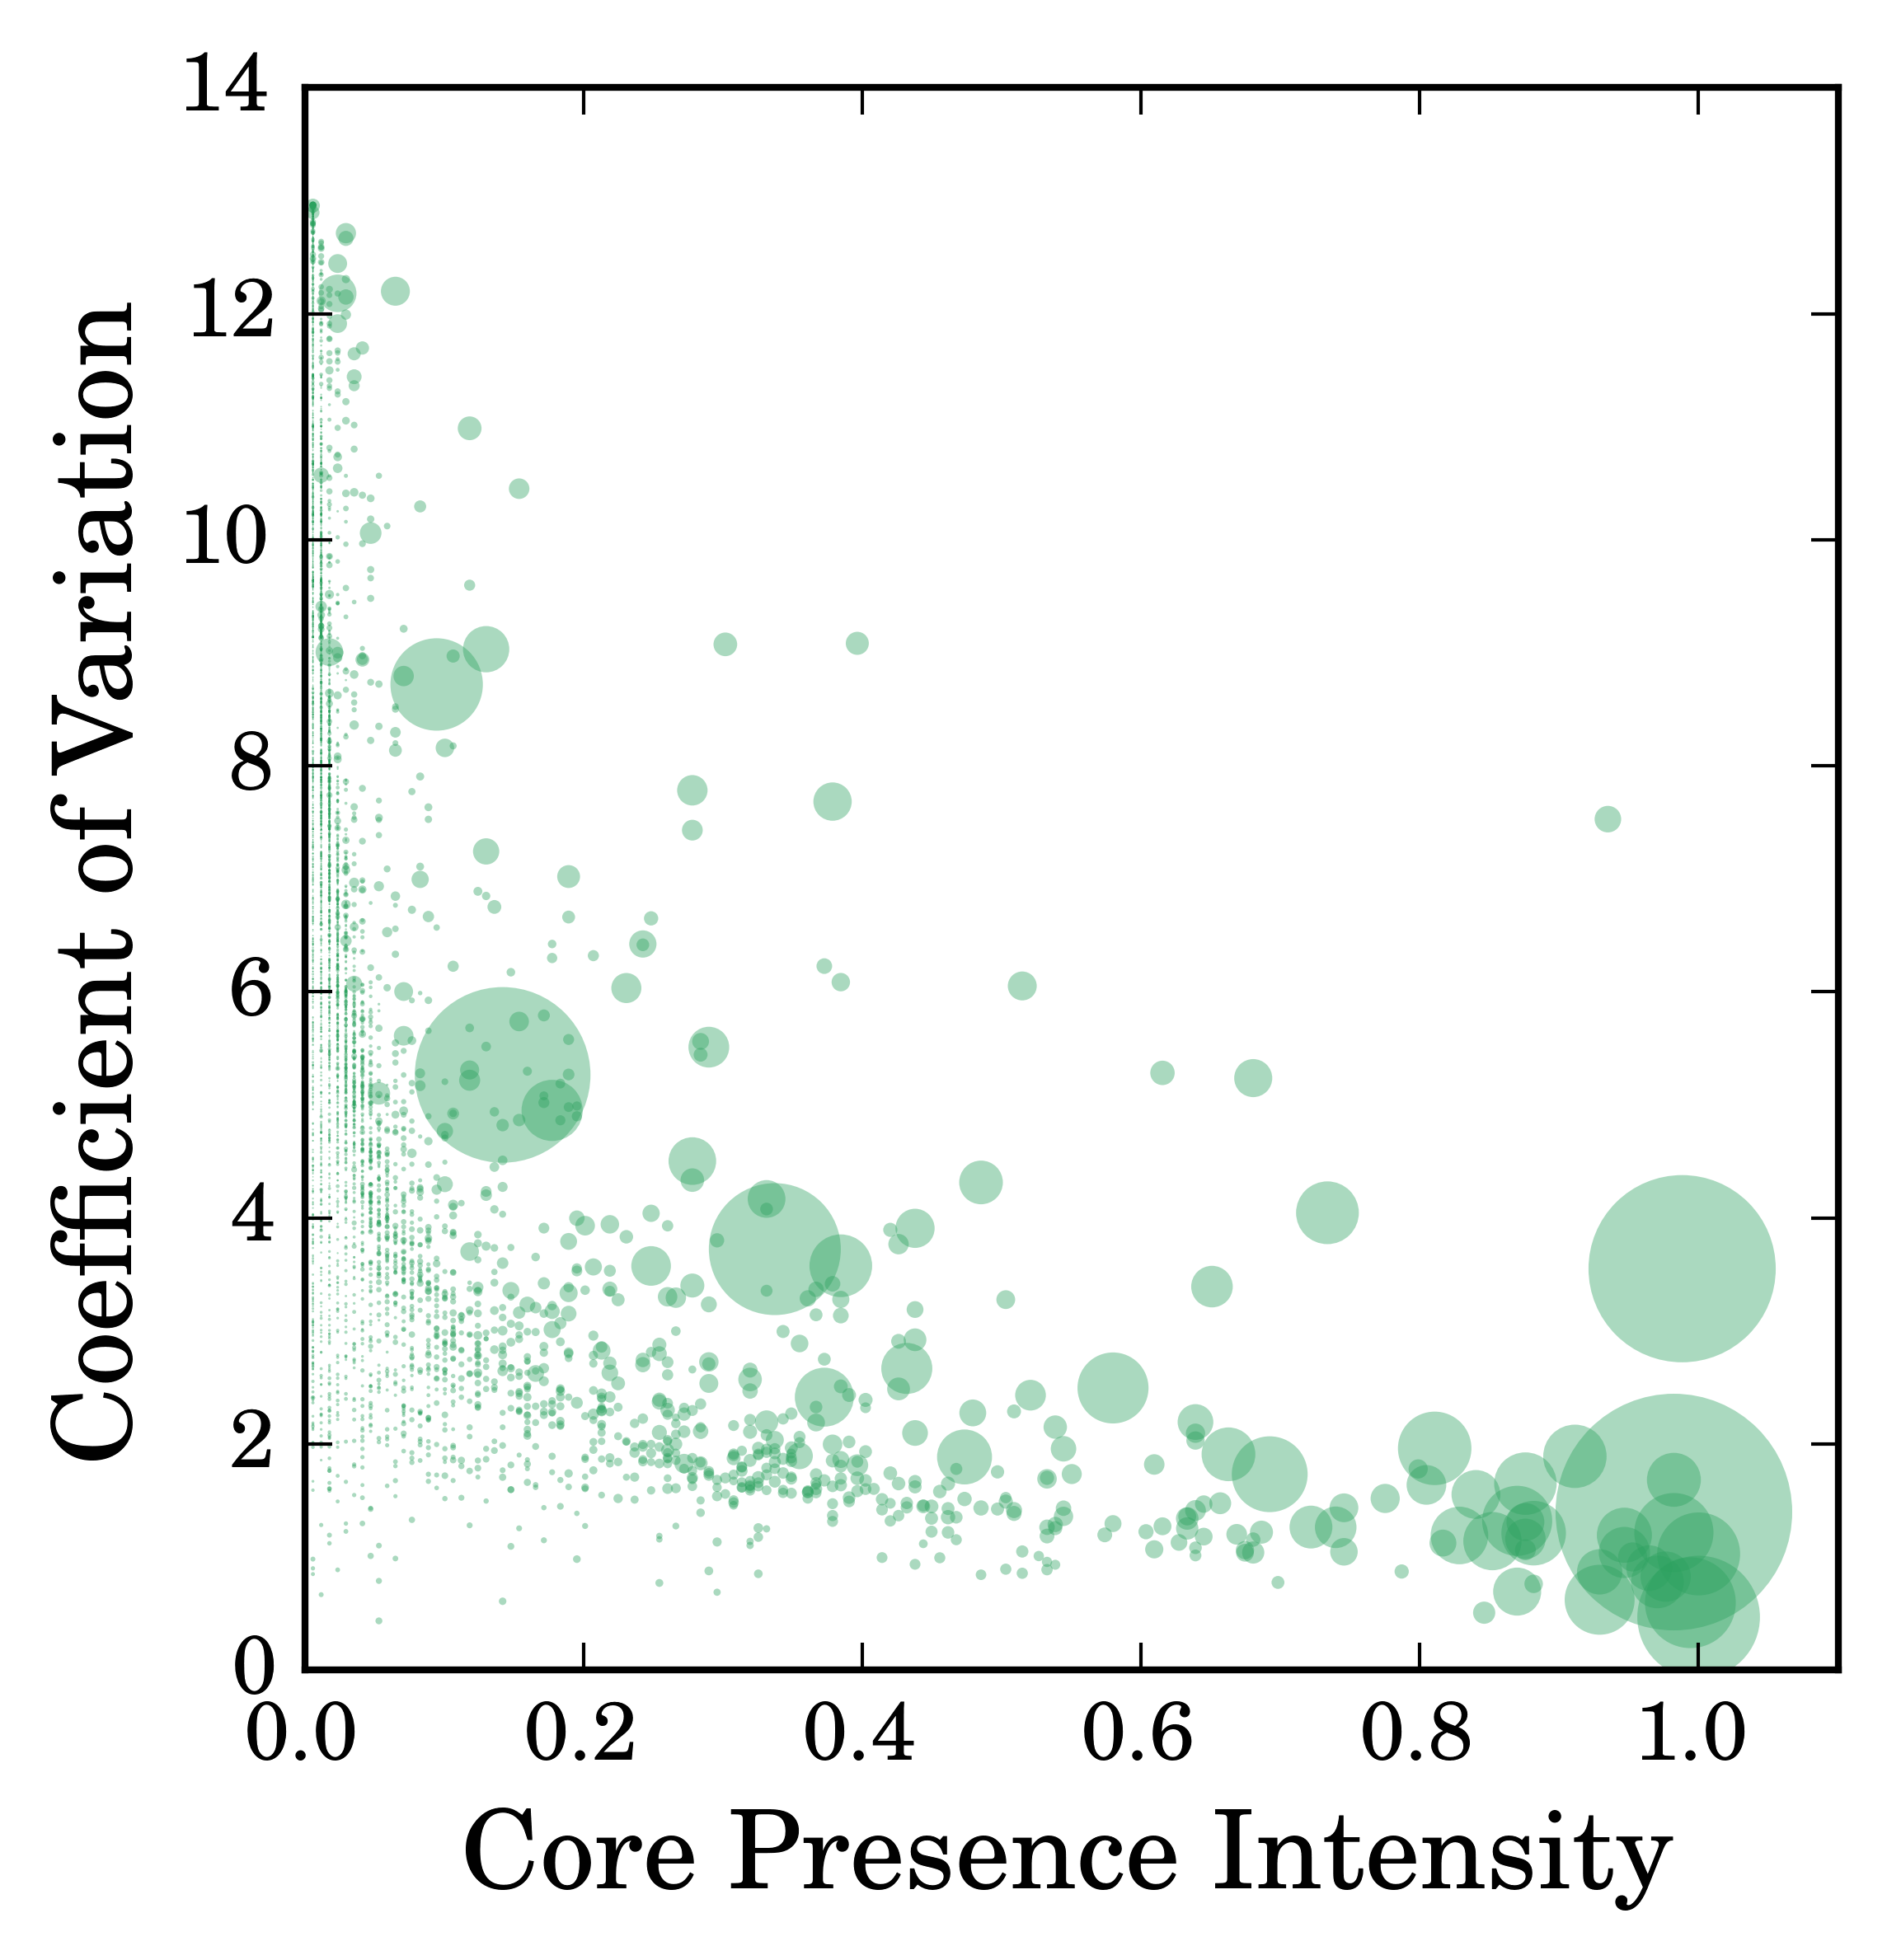
\includegraphics[width=\textwidth]{gfx/chap2/corre_cv_cp_sf.png}
                \caption{SF, 26907 prefixes}
                \label{fig:cv_cp_sf}
        \end{subfigure}
\caption{Relation between $I_{cp}$ over one week and $c_v$ of hour volume over the week from June 1st, 2015. Each circle stands for a prefix. Number of active prefixes plotted is each sub-graph throughout the week is also given. Circle size is proportional to the week volume fraction of the prefix the circle represents and is of the same scale for all networks.}
\label{fig:cv_cp}
\end{figure}
\begin{figure}\ContinuedFloat
	\centering
        \begin{subfigure}[b]{0.49\textwidth}
                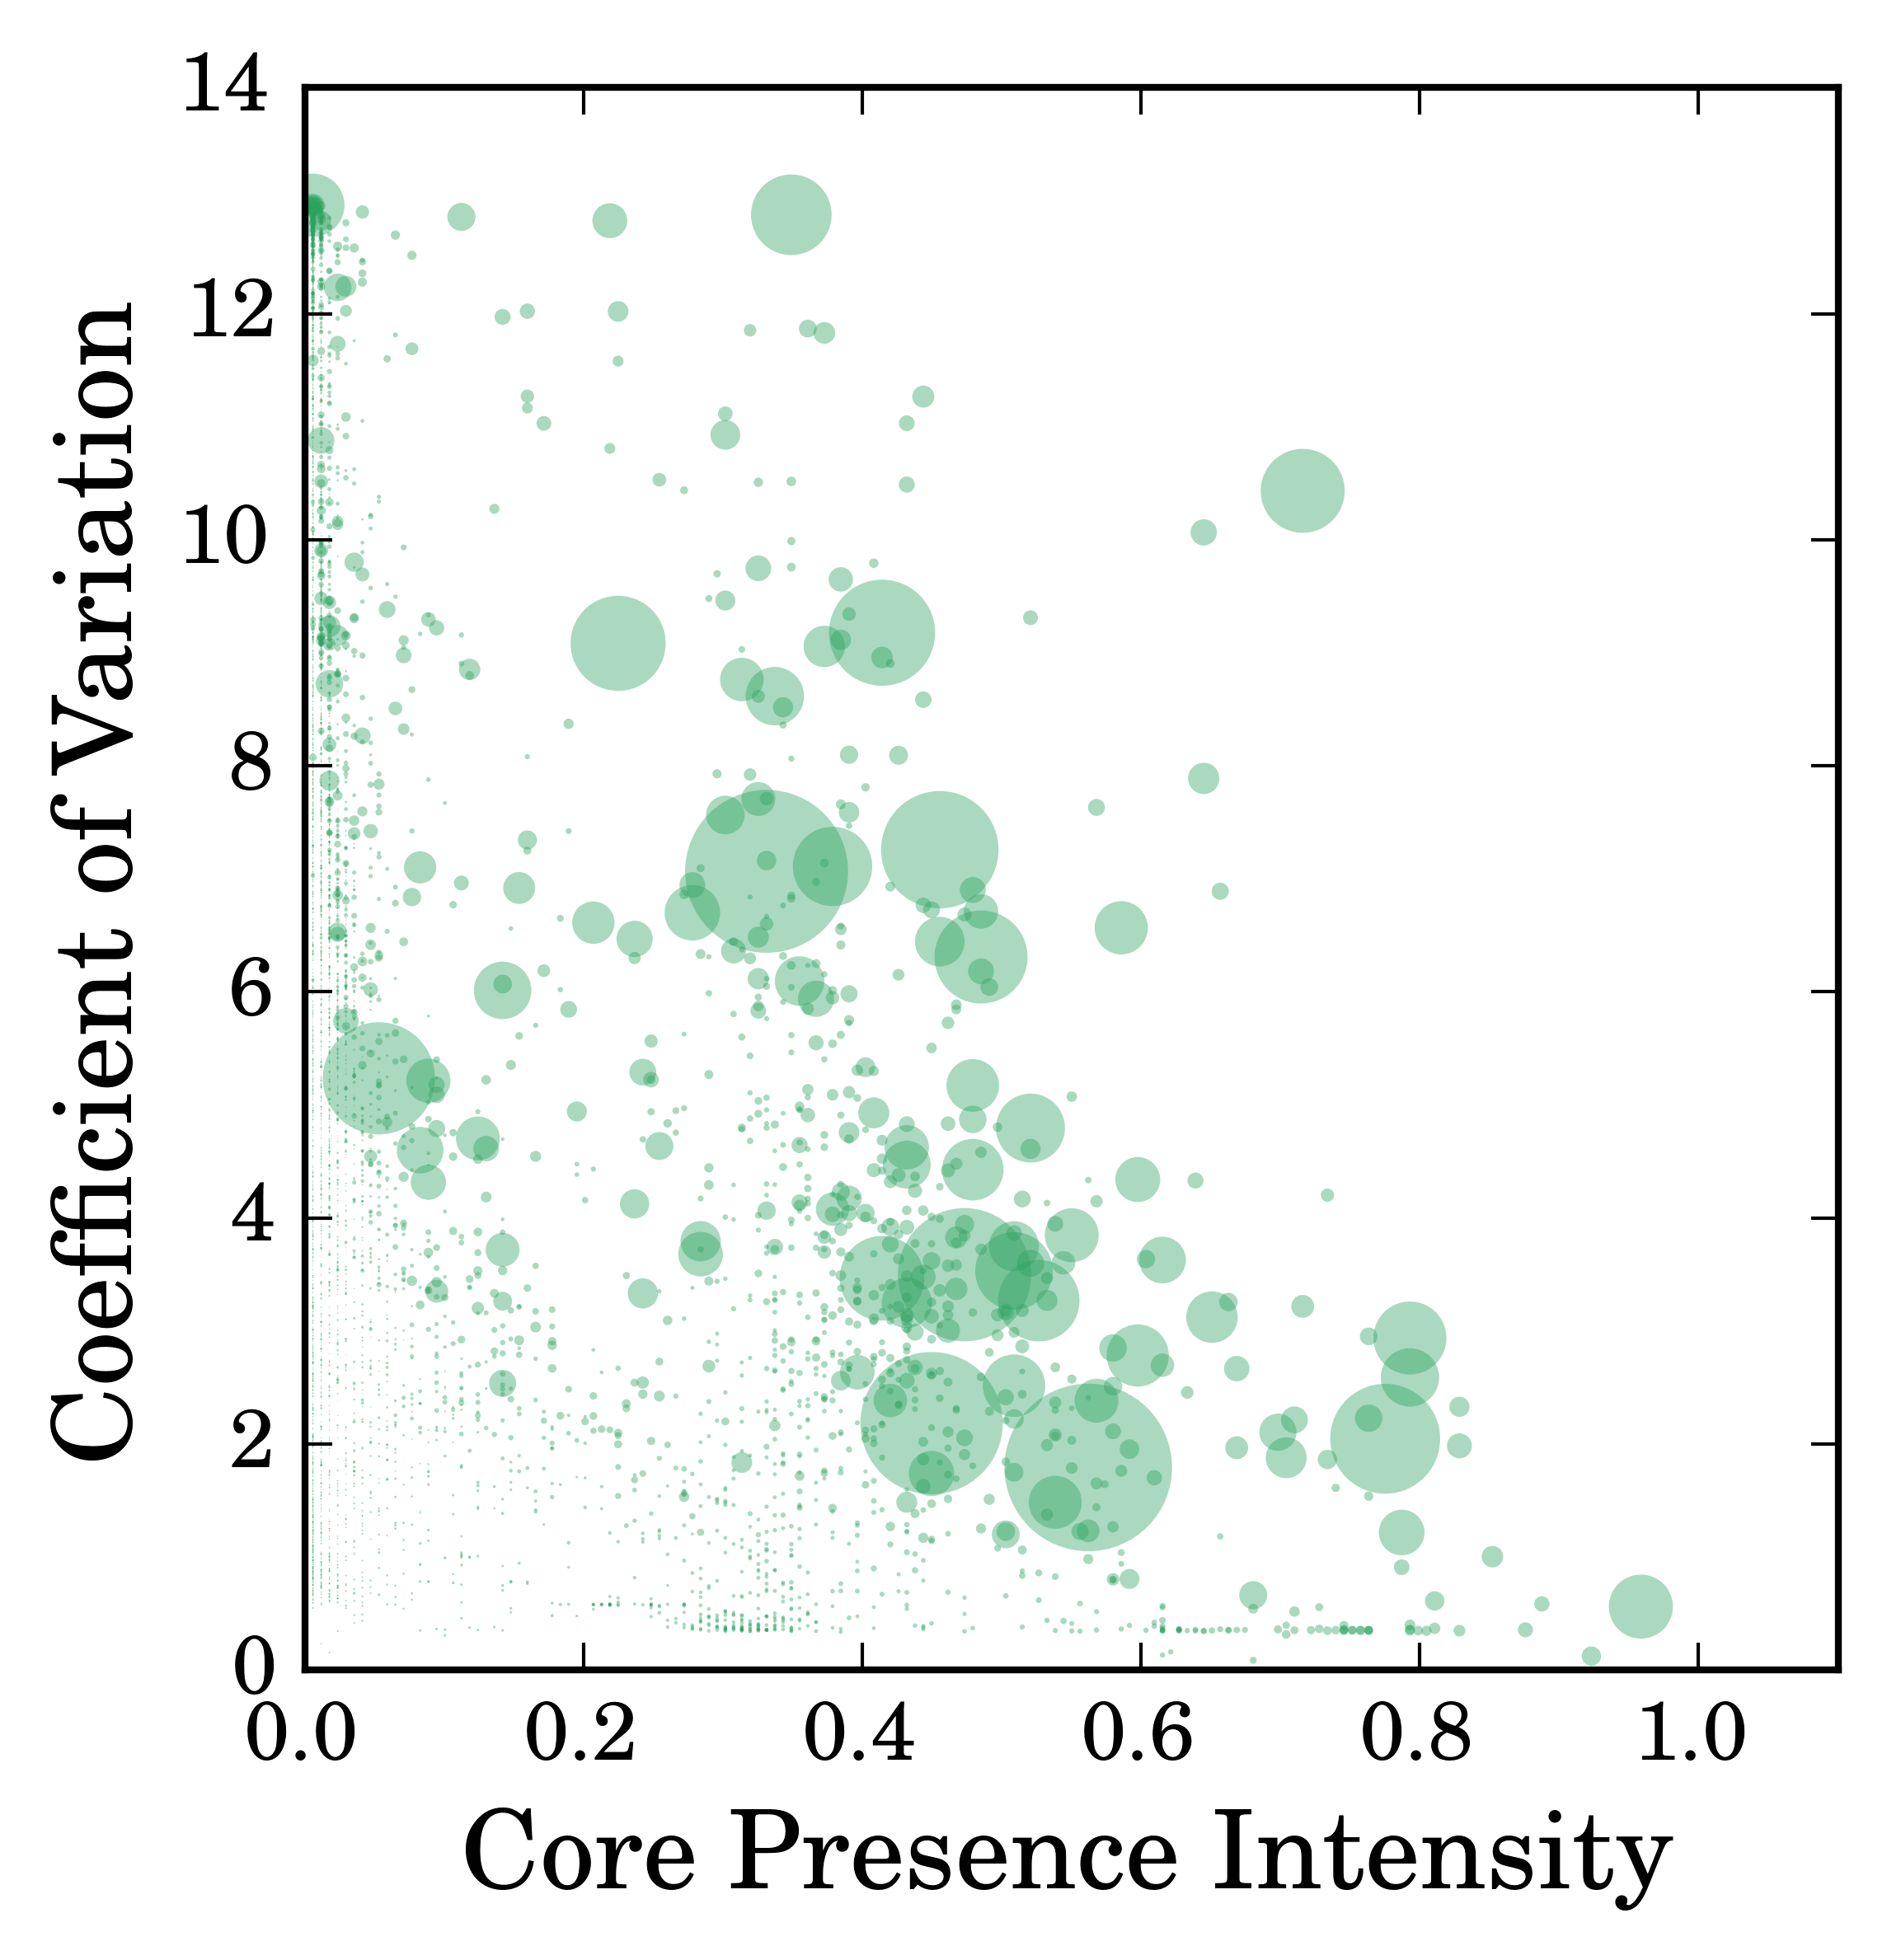
\includegraphics[width=\textwidth]{gfx/chap2/corre_cv_cp_sg.png}
                \caption{SG, 104425 prefixes}
                \label{fig:cv_cp_sg}
        \end{subfigure}
        \begin{subfigure}[b]{0.49\textwidth}
                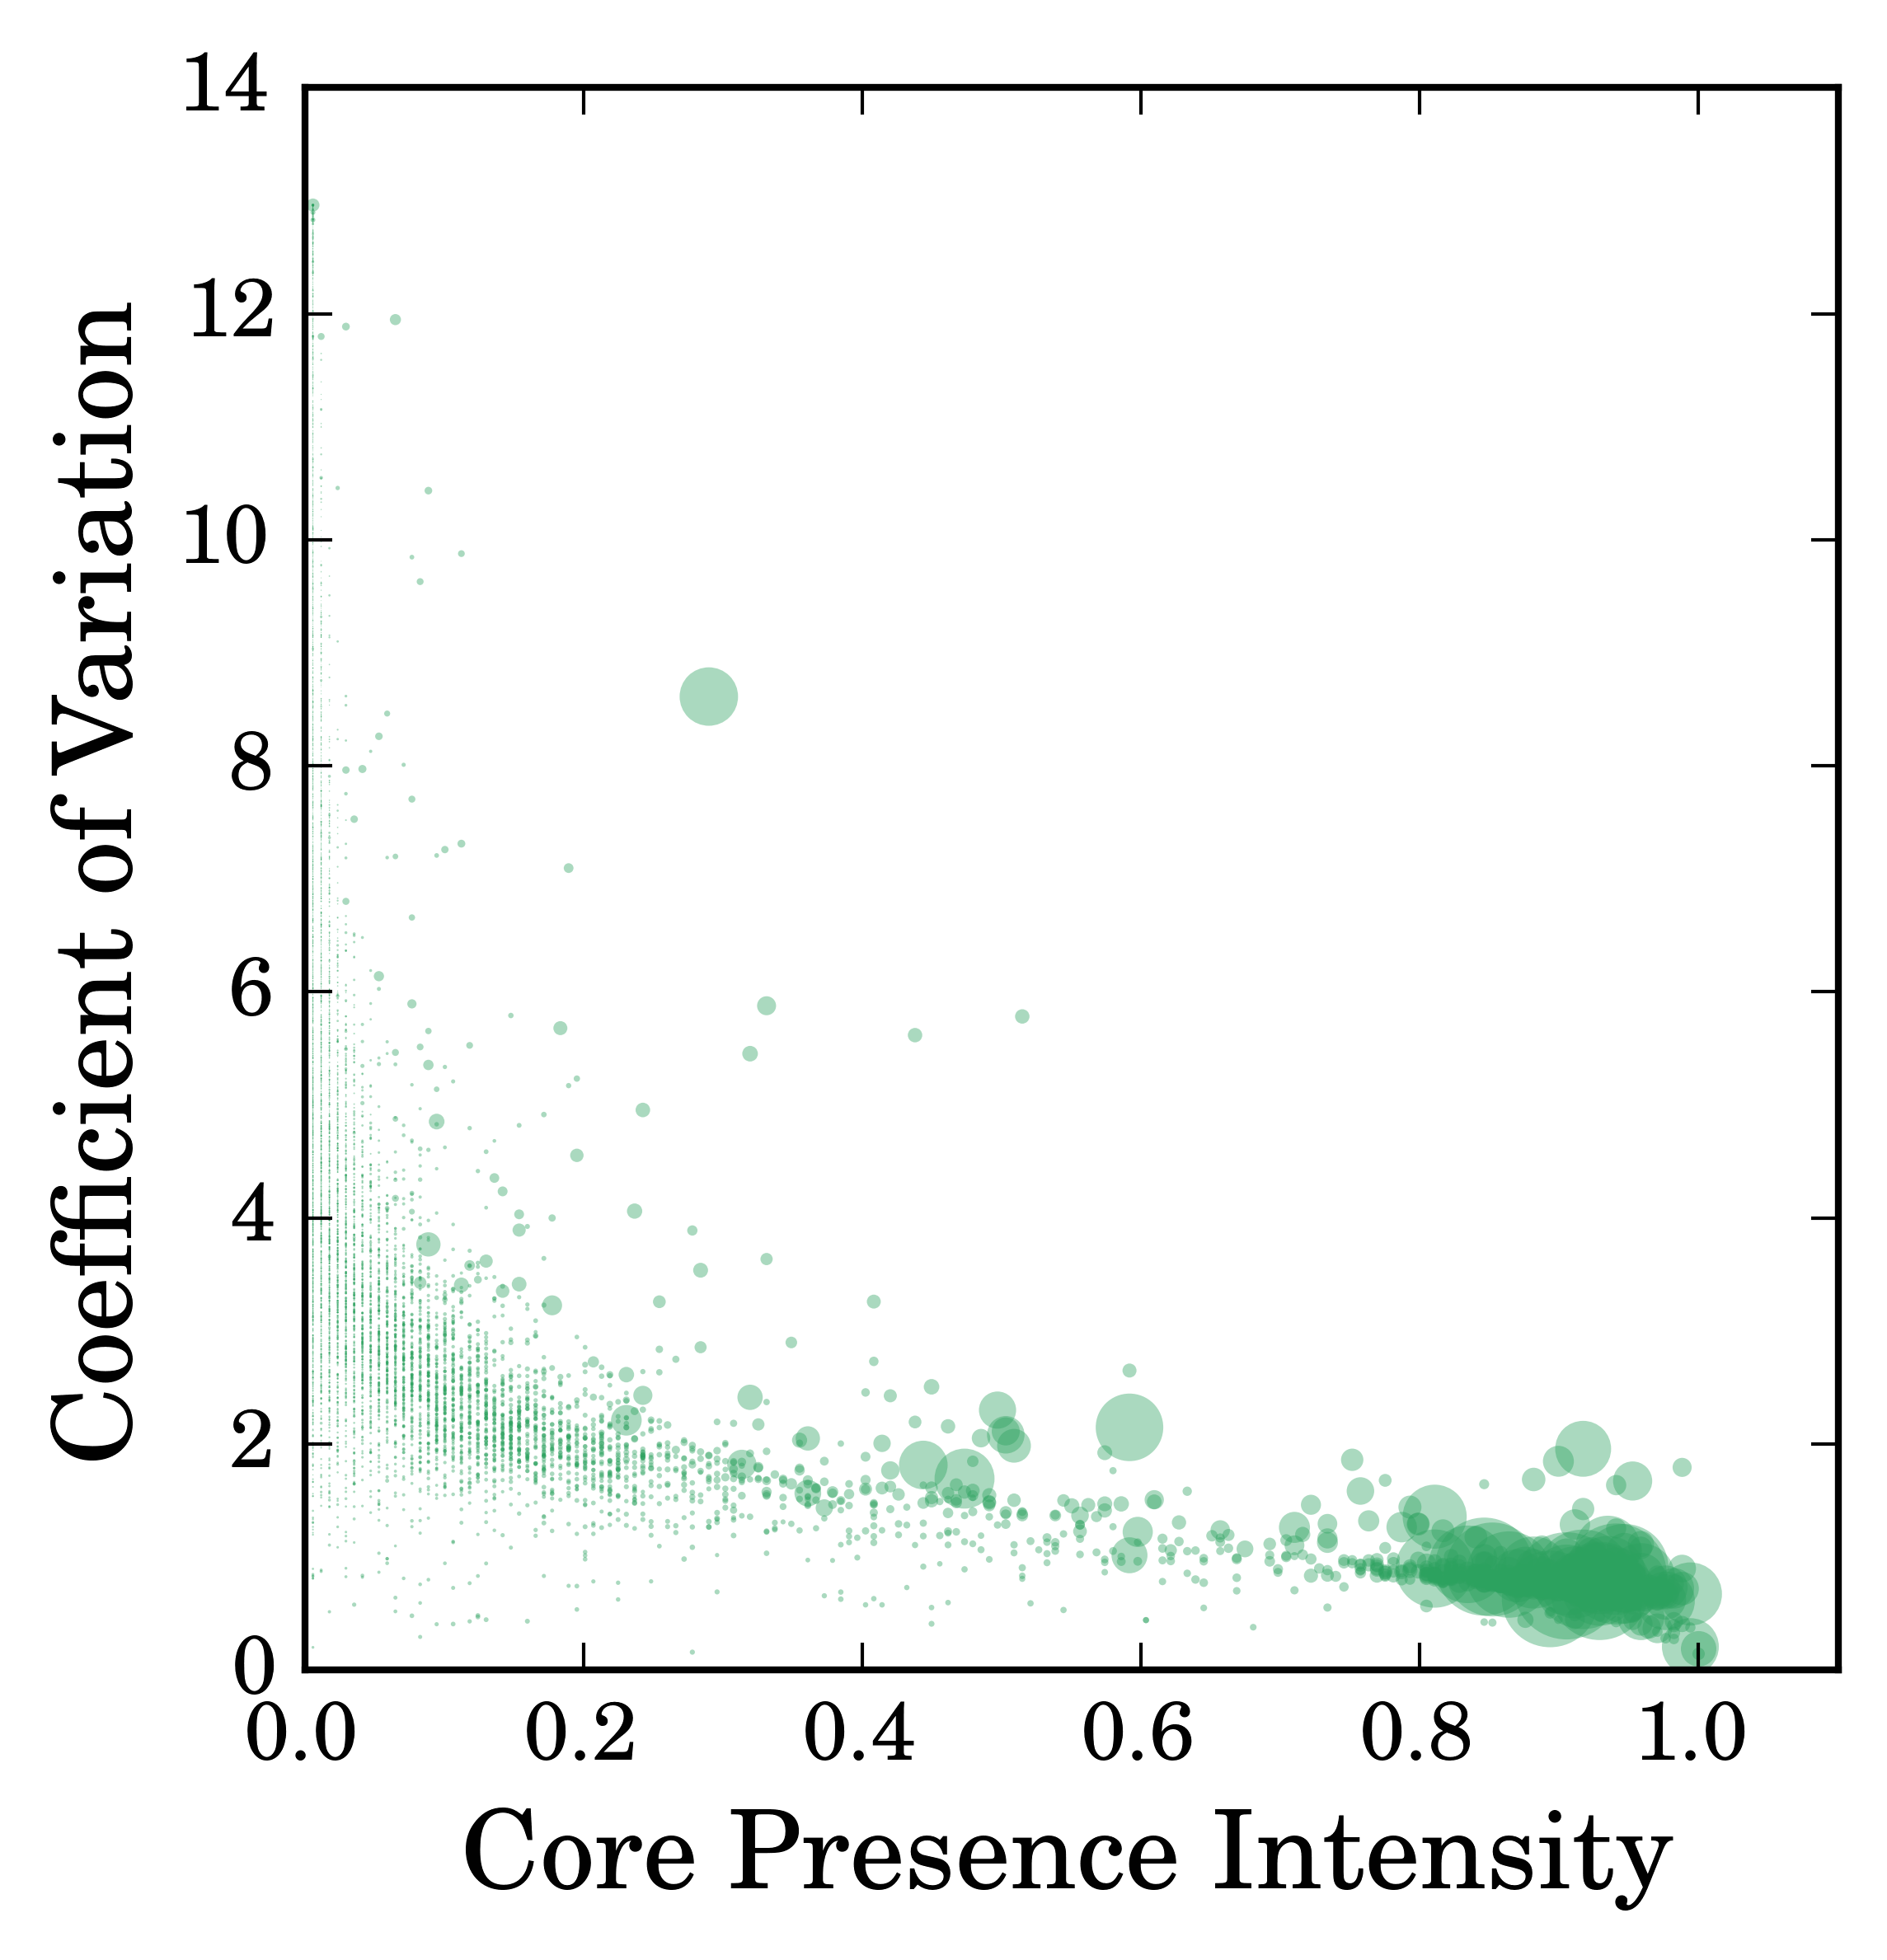
\includegraphics[width=\textwidth]{gfx/chap2/corre_cv_cp_sh.png}
                \caption{SH, 52061 prefixes}
                \label{fig:cv_cp_sh}
        \end{subfigure}
        \begin{subfigure}[b]{0.49\textwidth}
                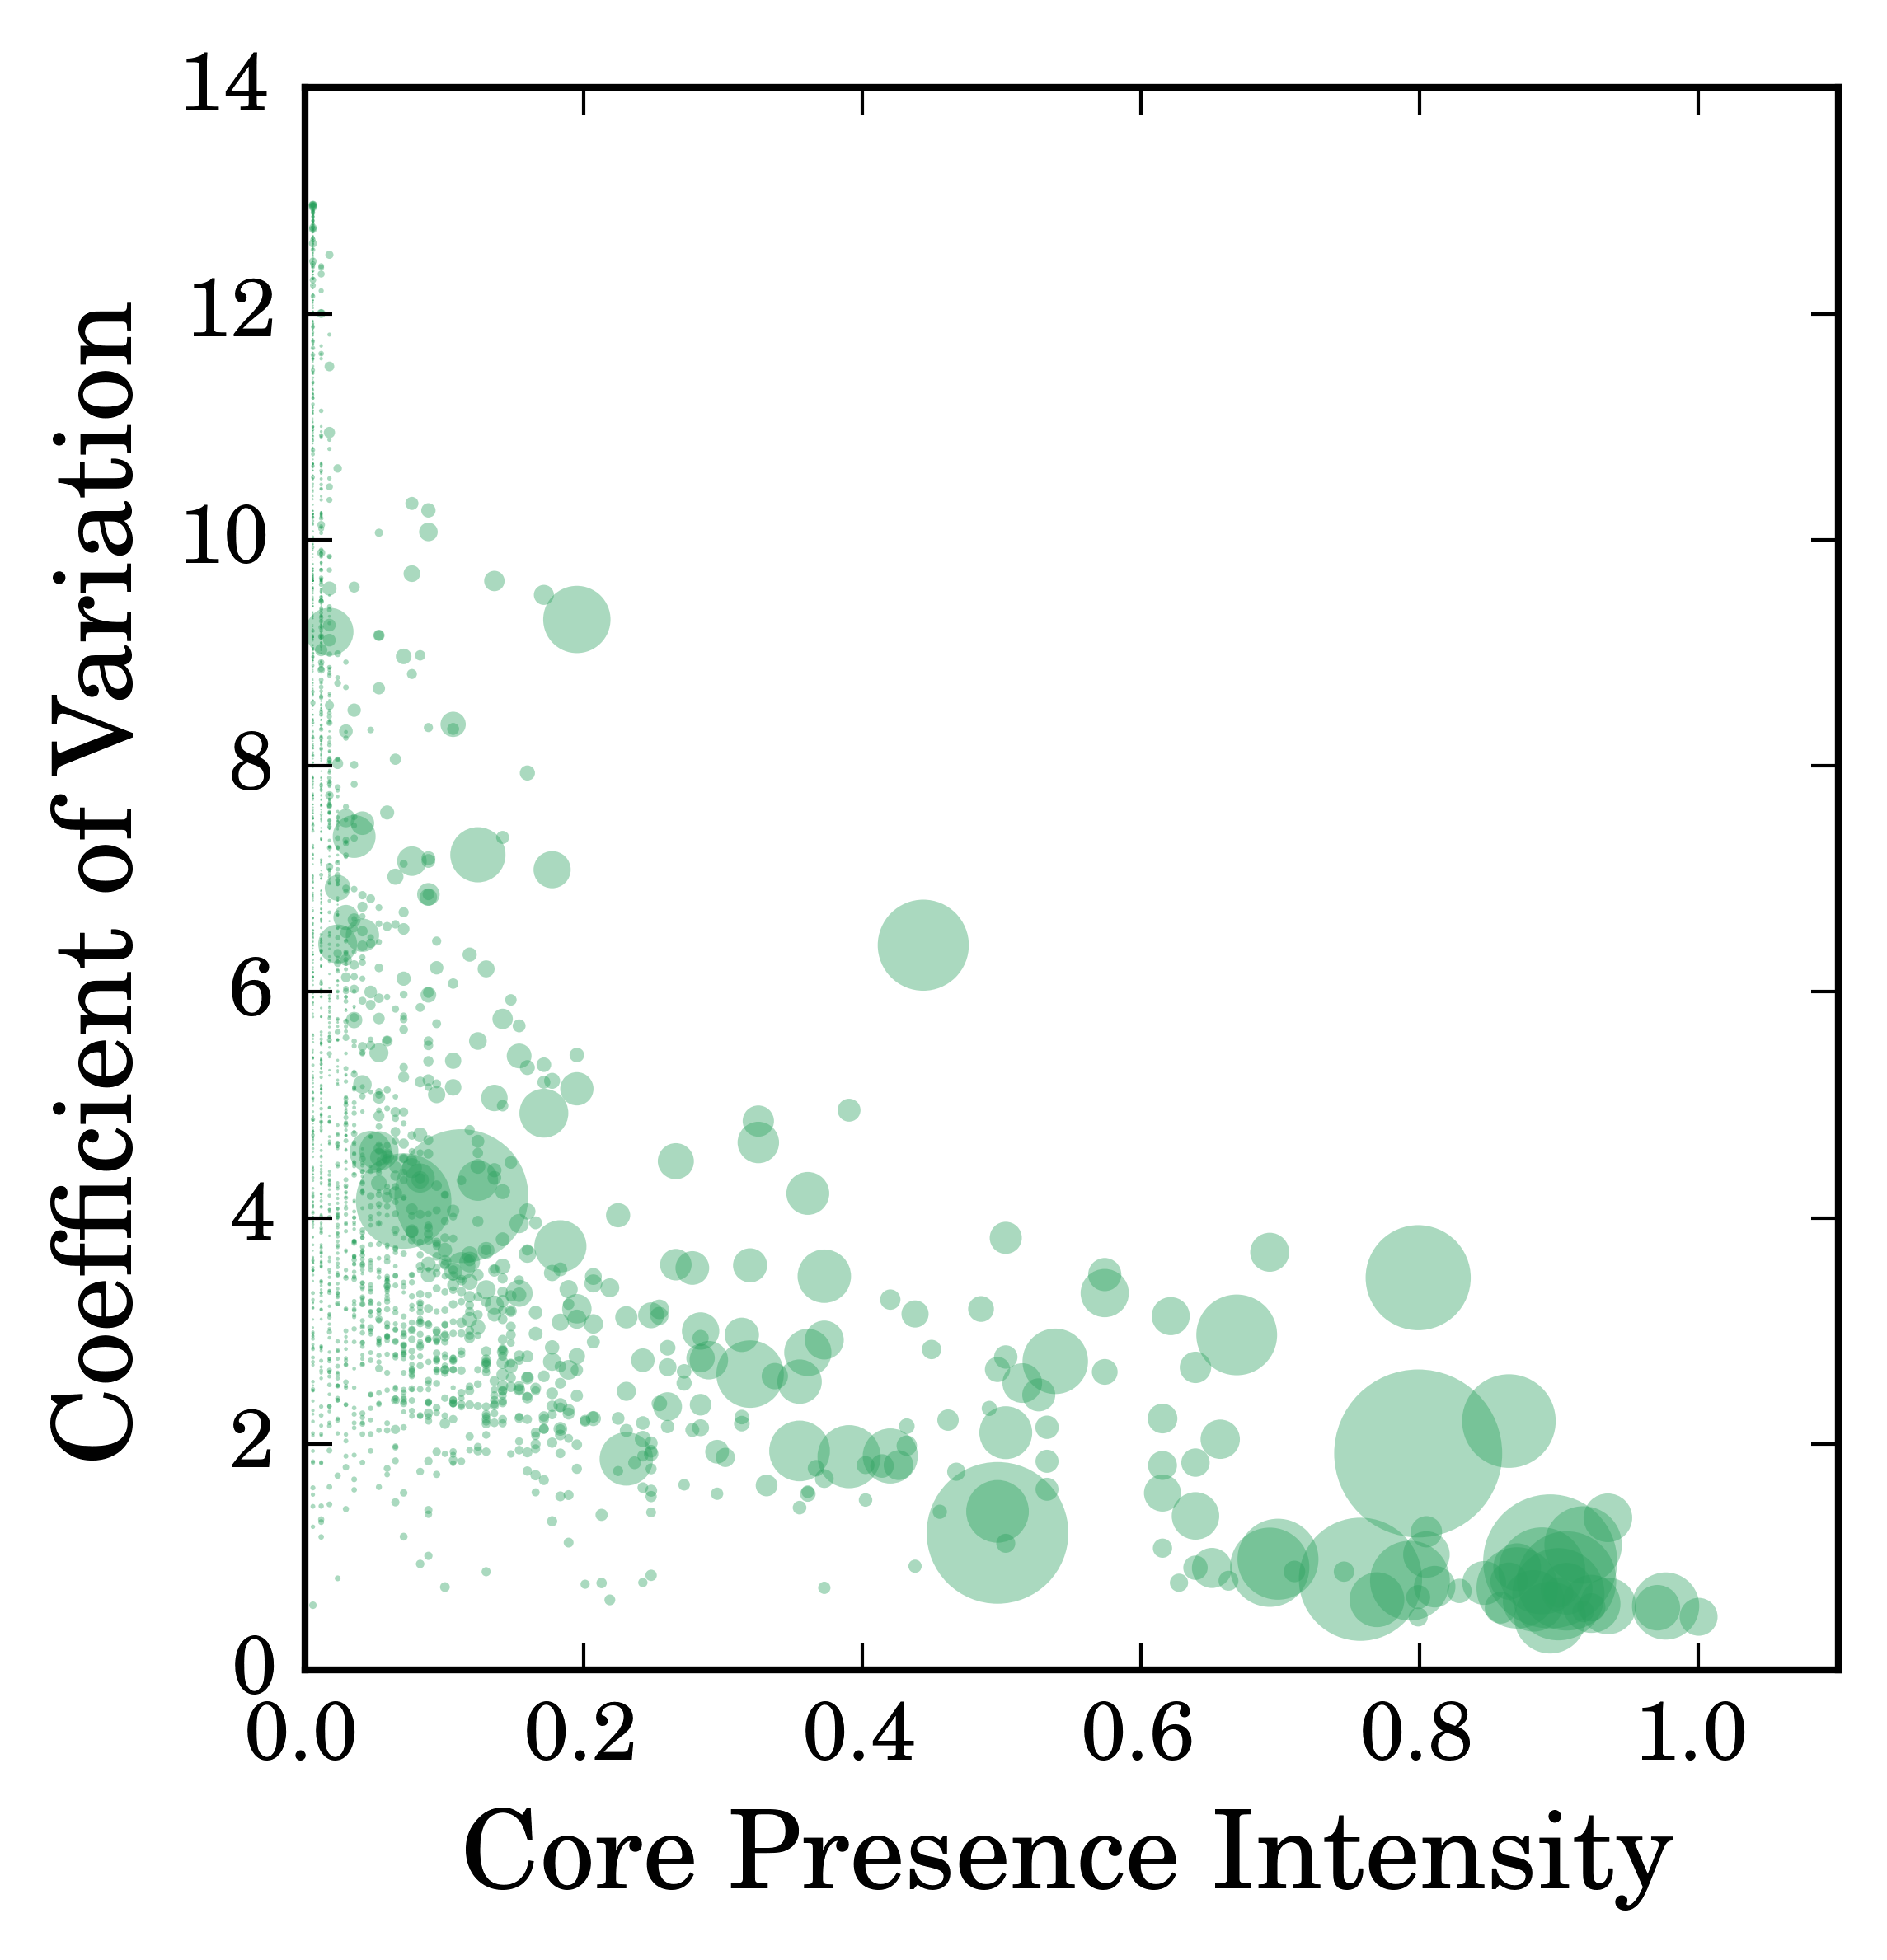
\includegraphics[width=\textwidth]{gfx/chap2/corre_cv_cp_si.png}
                \caption{SI, 14189 prefixes}
                \label{fig:cv_cp_si}
        \end{subfigure}
\caption{(cont.) Relation between $I_{cp}$ over one week and $c_v$ of hour volume over the week from June 1st, 2015.}
\label{fig:cv_cp_cont}
\end{figure}

For the sake of comparison, we study as well the correlation between these two metrics: $c_v$ %of hour volume throughout the week 
and $I_{cp}$ in Figure~\ref{fig:cv_cp}.
In the figure, each circle represents a prefix and its radius is proportional to the prefix's week volume share.
The biggest circles mostly concentrate in the lower right corner (small $c_v$ and large $I_{cp}$) of each sub-graph, which corresponds to the remarks made previously.
However, some exceptions exist especially on SC (but also SF, SG and SI).
On corresponding sub-graphs, we notice big circles having low $I_{cp}$ and relatively high $c_v$.
These prefixes bring significant week volume share within a short duration, which makes predictive prefix selection difficult. 
This observation leads the discussion on traffic burstiness later on.
Finally, it's not a surprise to see that the $c_v$ of prefixes with big week volume is, to a certain extent, inversely correlated to their $I_{cp}$.
%That is, when a prefix is associated with larger week traffic volume, chances are it has smaller variation in hour volumes and presents more often in the \textit{core} set.

\subsubsection{A view at hour interval}
\begin{figure}
\centering
        \begin{subfigure}[b]{0.85\textwidth}
                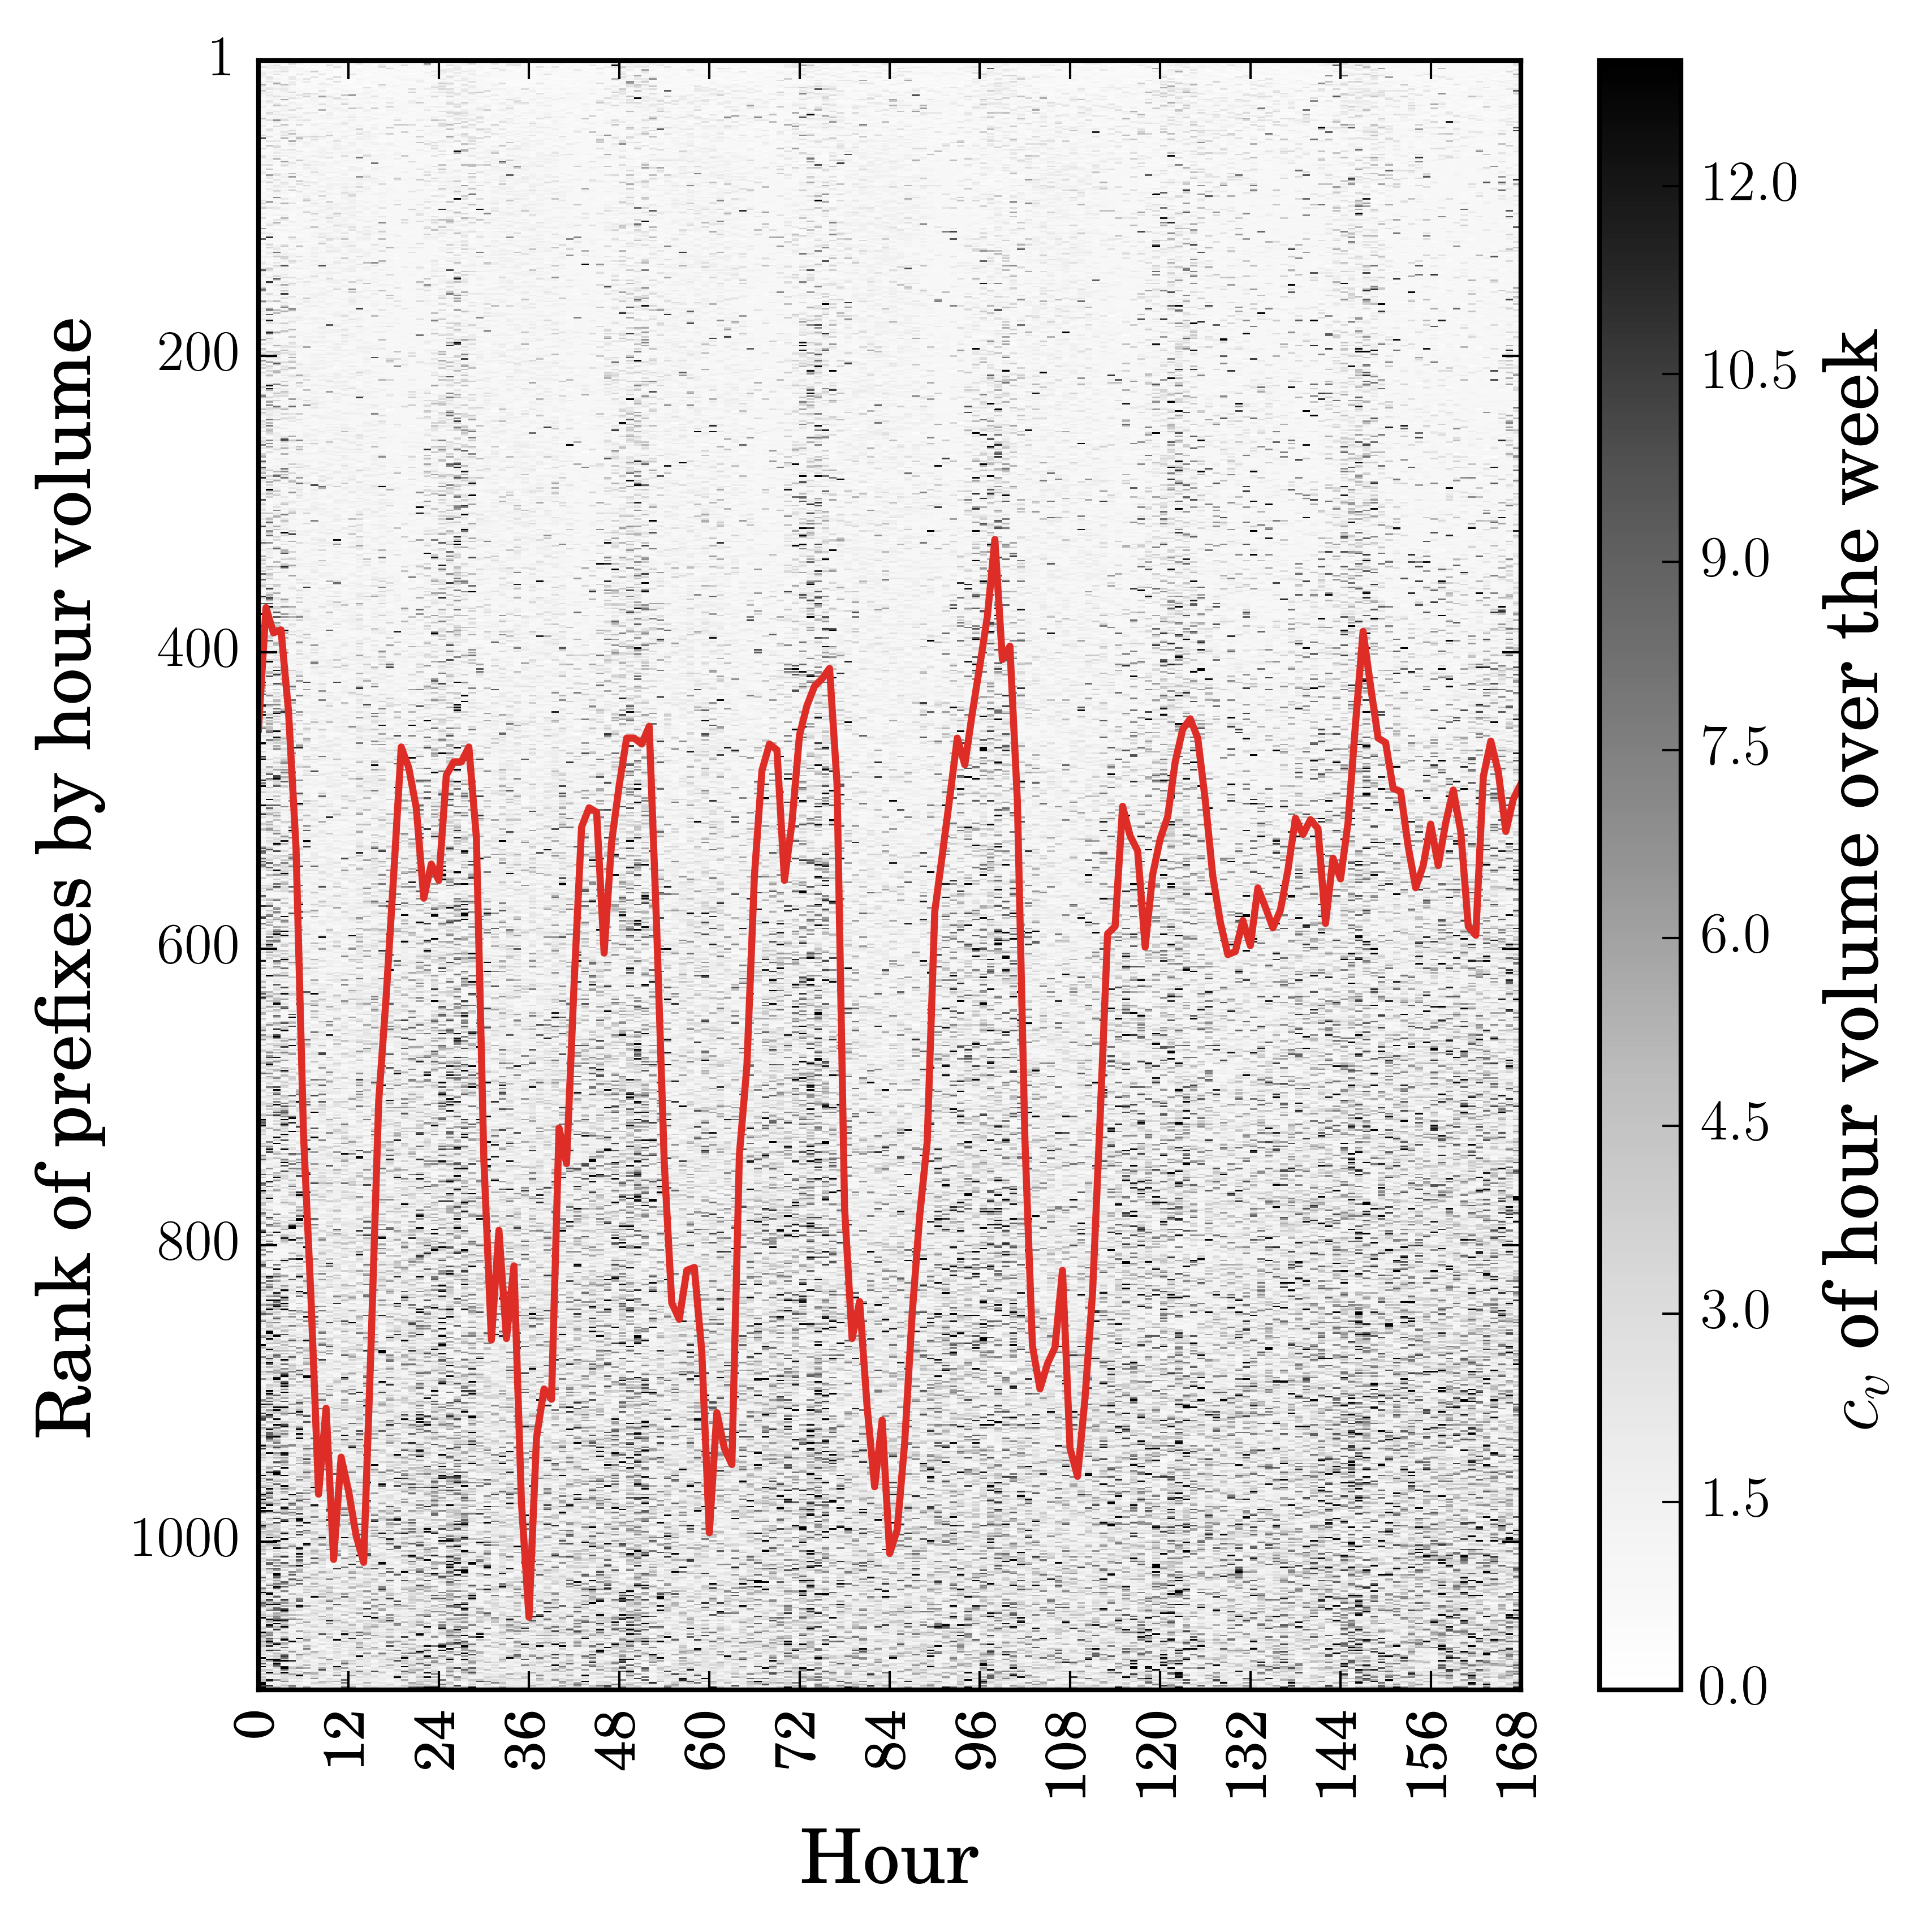
\includegraphics[width=\textwidth]{gfx/chap2/cv_mat_sa.png}
                \caption{$c_v$}
                \label{fig:cv_mat_sa}
        \end{subfigure}
        \begin{subfigure}[b]{0.85\textwidth}
                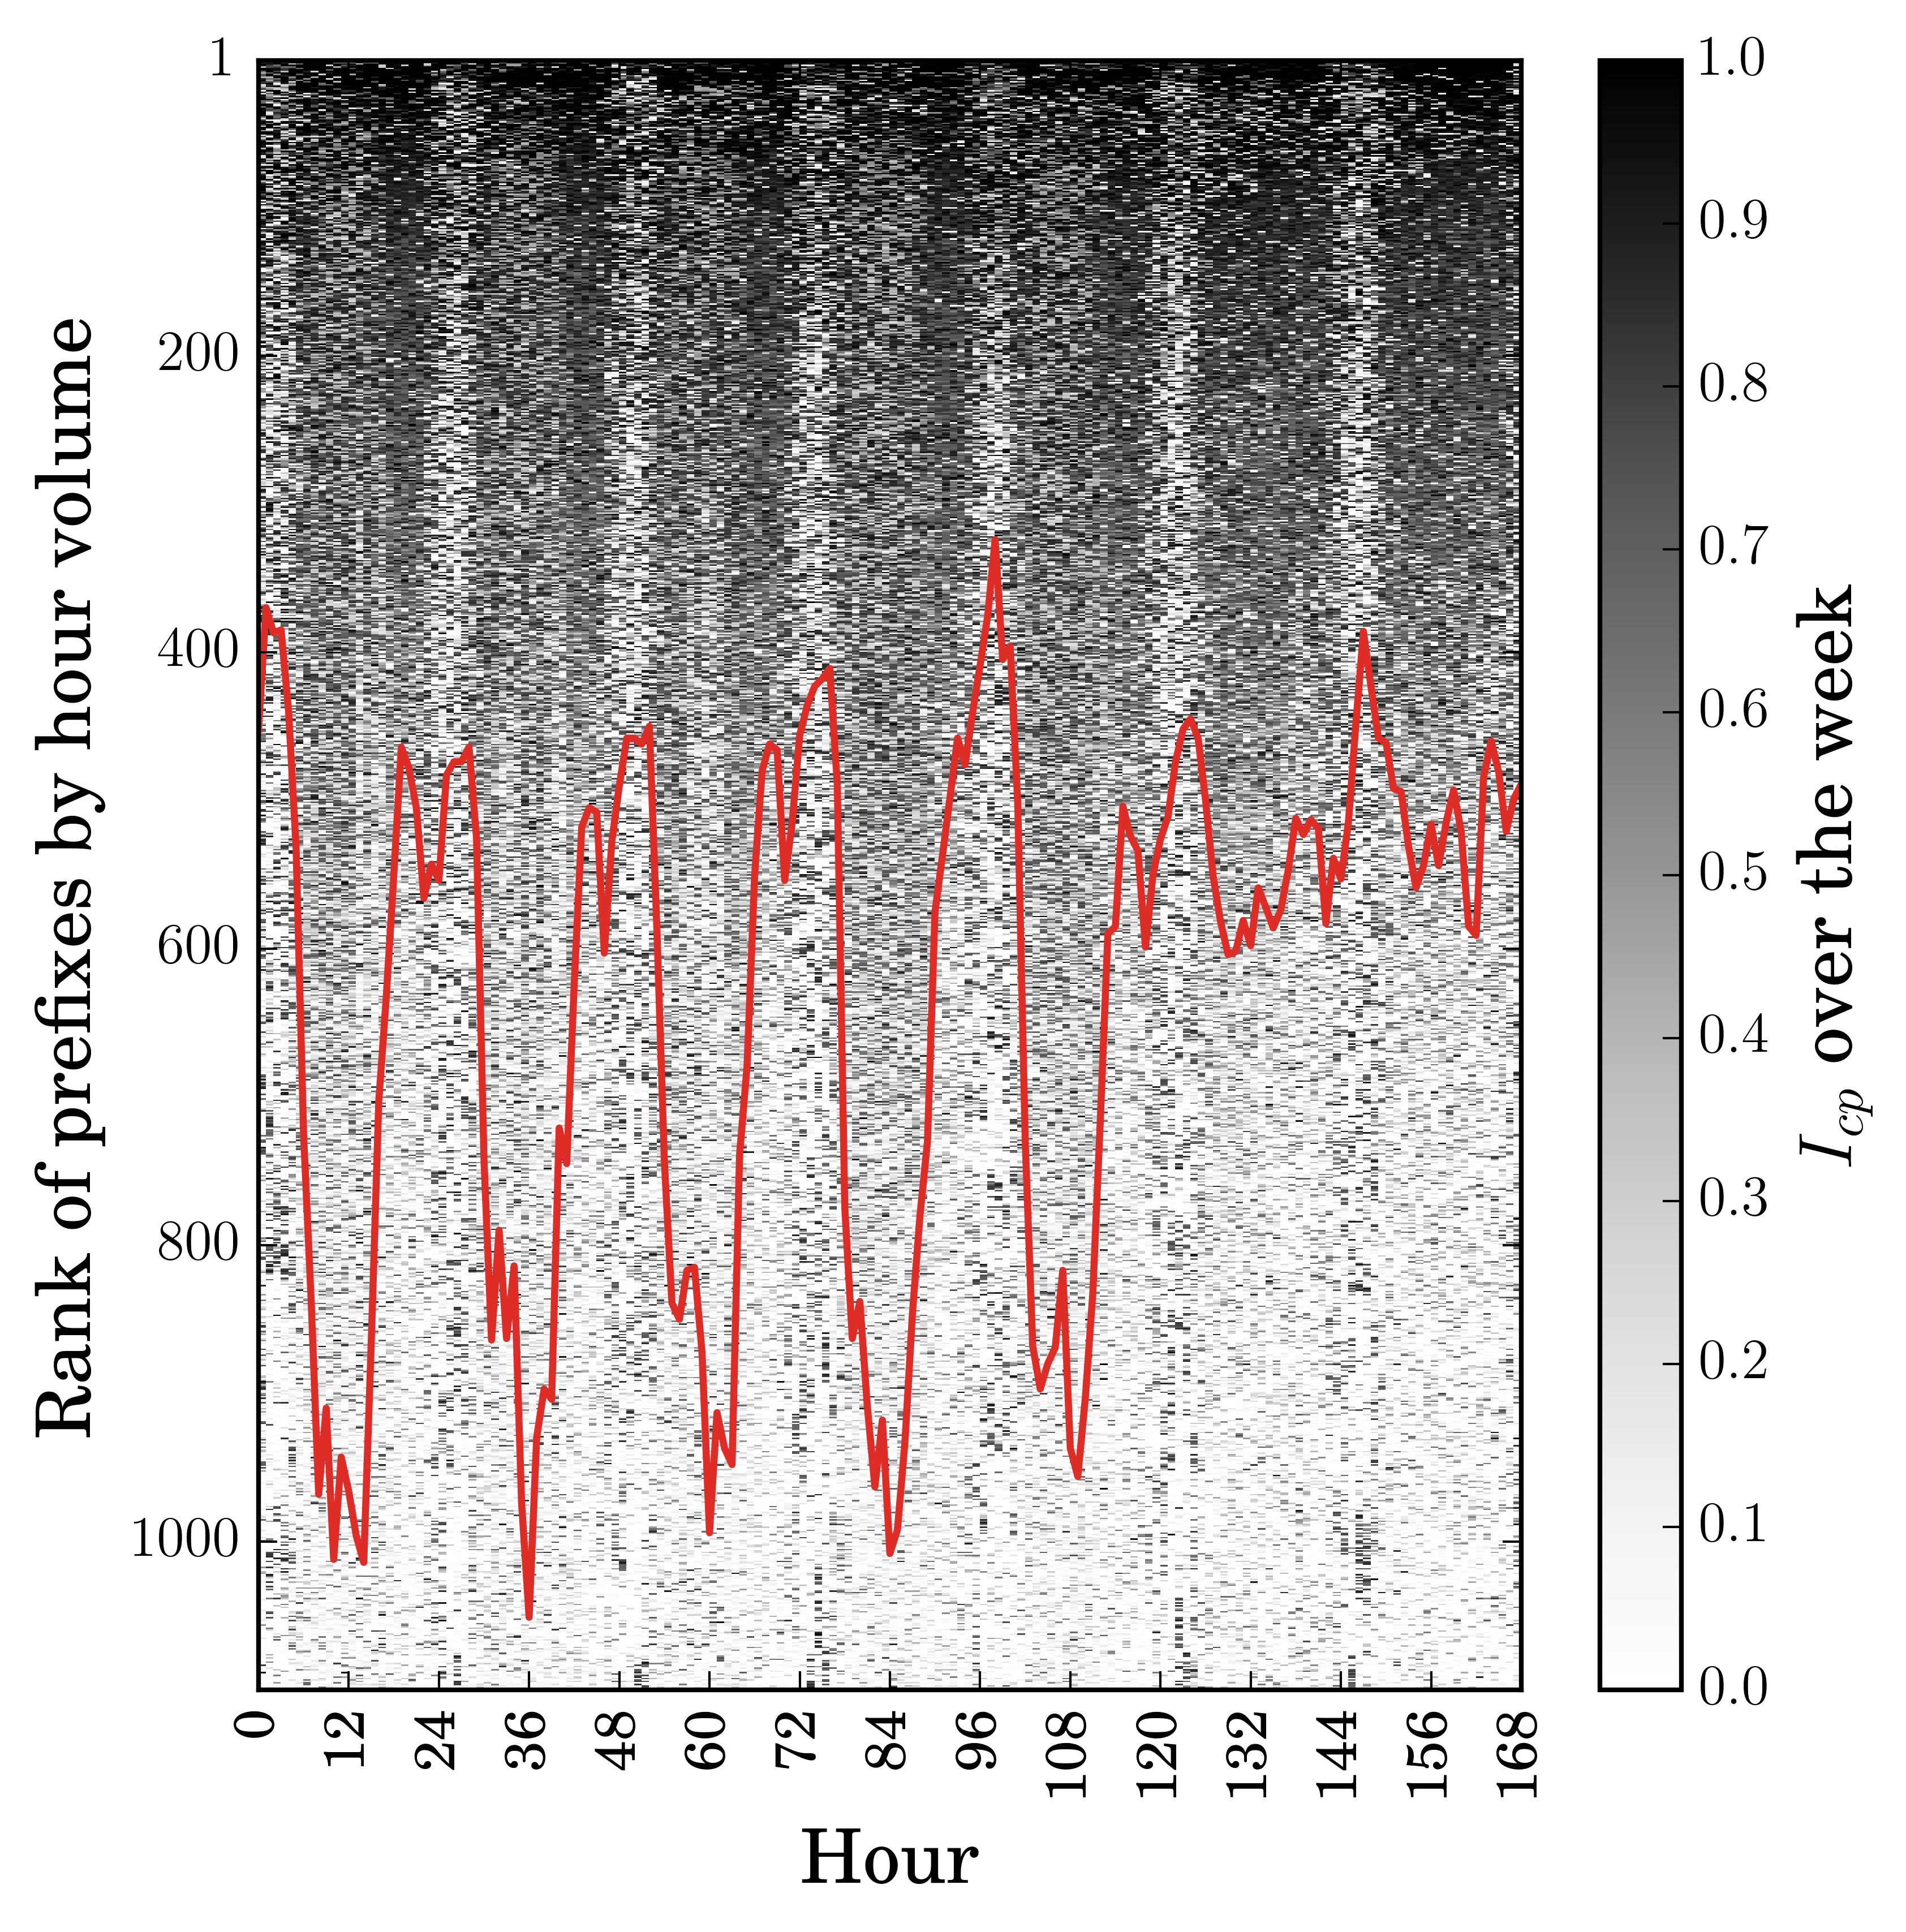
\includegraphics[width=\textwidth]{gfx/chap2/cp_mat_sa.png}
                \caption{$I_{cp}$}
                \label{fig:cp_mat_sa}
        \end{subfigure}
\caption{$c_v$ and $I_{cp}$ over one week for top ranked prefixes at each hour on SA. Prefixes are ranked by their hour volume along the column (big prefixes at the top). Their $c_v$ or $I_{cp}$ over the week are represented by the grey scale. Red line indicates the number of prefixes in \textit{core} prefix set each hour.}
\label{fig:cv_cp_mat}
\end{figure}

%\marginpar{traffic dynamism at finer time resolution}
The above analyses at week scale conclude that most prefixes that are associated with a big week volume  tend to be stable in hourly variation and present often in \textit{core}.
Here, we explore the prefix volume dynamism at hour resolution by visualizing each prefixes weekly $c_v$ and $I_{cp}$ in Figure~\ref{fig:cv_cp_mat}.
In the figure, each column (every hour in the week has it column) corresponds to top prefixes ranked by their \textbf{hour volumes}.
Large volume prefixes are at the top of the graph with small ranks.
Within the column, a grey scale tile is assigned to each prefix to portrait its $c_v$ or $I_{cp}$ over the week.
Prefixes above the red line are those composing \textit{core} at each hour.
Only graphs for SA are shown. 
They presents most informative patterns, since less bursty traffic is from SA.
We notice that the \textit{core} size varies regularly on a daily base.
During peak hours, the \textit{core} size can be twice its minimum value.
This diurnal pattern is another illustration of different traffic concentration level at different moments, a phenomenon first revealed with Figure~\ref{fig:sa_cdf_multi_time}.
Moreover, the \textit{core} size seems to show a different pattern then the rest of the days.
Since these two days are actually a weekend, this change suggests probably a potential hebdomadal traffic cycle.

%\marginpar{observations from $c_v$ graph}
In the sub-graph for $c_v$ (Figure~\ref{fig:cv_mat_sa}), the area above the red line has observably lighter tone than the lower part. 
This implies that in each hour, prefixes in the \textit{core} have more stable hour volume variation, i.e. closer to its mean value,  than those outsiders with little volume significance.
Moreover, the figure demonstrates as well a time-of-day pattern for $c_v$ values. 
During late night and early morning, prefixes in the \textit{core} have deeper color, thus more volatile, than those in the day time.
This indicates that important prefixes composition are not quite the same during these two periods.
The above described phenomenon are sometimes a little bit more difficult to perceive on networks with more bursty traffic. 
Anyhow, for those `bursty' networks, the tone of the \textit{core} area is not visibly darker.
It means the hourly volume time series for large prefixes are not obviously less stable.
We should all the same be able to pick them out using their mean value.
The lack of clear diurnal pattern for some networks is possibly related to their business type and client activity, which is out of the scope of this work.

%\marginpar{observations from $I_{cp}$ graph}
When it comes to $I_{cp}$ (Figure~\ref{fig:cp_mat_sa}), it is true for all networks that top ranked prefixes each hour are more likely to frequently appear in the \textit{core} prefix set.
That is deeper color at the top of the graph.
However, we can witness light spots each hour in the upper part of the graph, which corresponds to bursty traffic.
Time-of-day pattern from $I_cp$ values can also be clearly observed. 
It confirms again that prefixes active over night are different from those during the day time.


\subsection{Quantitative index of traffic burstiness}
Previous explorations have shown that the predictability of traffic volume from a client network is related to its traffic burstiness.
In order to describe burstiness in a quantitative manner, we define the index $\beta(P)_h$, for a prefix $P$ at certain hour $h$ as:
\begin{equation*}
\beta(P)_i = \begin{dcases*}
         -\log(I_{cp}(P)) \times vp(P)_i & if $I_{cp}(P) > 0$\\
        0 & if $I_{cp}(P) = 0$,
        \end{dcases*}
\label{eq:beta}
\end{equation*}
where $vp(P)_h$ is the hour volume percentage (among all active prefixes) of prefix $P$ at hour $h$.
The logarithmic term applied on $I_{cp}$ aims at amplifying the volume contribution of prefixes with rare \textit{core} presence, and attenuating the influence of prefixes being intensively in the \textit{core}.
A large $\beta$ value indicates that it is hard to predict the volume associated with this prefix while representing a significant hour volume.

In order to estimate the overall burstiness of all prefixes at hour $h$ for a network, we sum up the $\beta(P)_h$ for each $P$ inside the \textit{core} of that hour: more formally, 
%Wenqin: notation for $\beta(P)_i$ is not right
\begin{equation*}
BI_h = \sum_{P \in \textit{core}_h} \beta(P)_h.
\label{eq:bi}
\end{equation*}
%Wenqin: notation for $\beta(P)_i$ is not right
For all the networks, we estimate their traffic burstiness with the mean and maximum of $BI$ value series over the week. The results are given in Table~\ref{tab:bi}. The maximum $\beta$, contribution from a single prefix, throughout the week is also given.

\begin{table}[!htb]
\centering
\footnotesize
\begin{tabular}{cccc}\toprule
\textbf{Network} & \textbf{Mean $BI$} & \textbf{Max $BI$} & \textbf{Max $\beta$}\\
\midrule
SA & 14.61 & 37.79  &  7.44\\
SB & 31.09 & 46.85  &  4.08\\
SC & 40.57 & 145.07 &  145.05\\
SD & 42.14 & 69.34  &  18.10\\
SE & 20.91 & 44.30  &  20.17\\
SF & 44.10 & 98.69  &  78.77\\
SG & 51.21 & 125.41 &  102.05\\
SH & 15.91 & 35.06  &  16.29\\
SI & 38.59 & 85.47  &  56.56\\
\bottomrule
\end{tabular}
\caption{Traffic burstiness.}
\label{tab:bi}
\end{table}

Mean $BI$ over the week measures the general burstiness of traffic, while maximum $BI$ describes the degree of burstiness in worst cases.
In accordance to the observation made from Figure~\ref{fig:cv_cp}, there are big volume prefixes with fairly low $I_{cp}$ on SC, SF, SG and SI, whence the much bigger maximum $\beta$ value.
What is less evident in Figure~\ref{fig:cv_cp} is that SD suffers actually a lot from bursty traffic, even more than SC on average.
For the rest networks, i.e. SA, SB, SE and SH, their mean $BI$ over the week is around 30 or lower. Their corresponding sub-graphs in Figure~\ref{fig:cv_cp} manifest as well much less big circles on the left side where $I_{cp}$ is low.
More specifically, SB suffers more from bursty traffic than SA, therefore bigger value in both maximum and mean $BI$ over the week.
This is however not easy to tell directly from Figure~\ref{fig:cv_cp}.
%which is in accordance with the observation that the tone of \textit{core} area of SB is lighter than that of SA in Fig~\ref{fig:cp_mat}.
Nonetheless, the maximum $\beta$ on SA is larger than that on SB, which is due to the fact that traffic on SB is more evenly distributed among active prefixes (see Figure~\ref{fig:traffic_dis_site}).
Therefore the faction of traffic associated to each prefix is generally smaller.
In short, we found this simple metric capable of describing the traffic burstiness of the networks studied.


\section{Predictive prefix selection}
\label{sec:sele}

\subsection{Candidate prediction metrics}

%\marginpar{prediction metrics inspired by traffic temporal dynamism studies}
Based on the previous observations, several approaches naturally emerges for the prediction of traffic volume ``importance'' of a prefix.
\paragraph*{Mean Volume}
With this metric, we predict that at hour $h+1$, the volume importance of prefix $P$ is indicated by it's mean hourly volume over the last $L$ hours, $MV(P,L)_{h+1} = 1/L \times \sum_{i = h-L+1}^{h} v(P)_i$.
It is based on the observations from Figure~\ref{fig:cv}, that top prefixes over the week tend to have smaller hourly volume variation around their mean volume.

\paragraph*{Core Presence Intensity}
The prediction could use $I_{cp}(P,L)_{h+1} = 1/L \times \sum_{i = h-L+1}^{h} cp(P)_i$, i.e. the \textit{core} presence intensity of the prefix over the last $L$ hours. It derives from the observation from Figure~\ref{fig:cpi}, that top prefixes by their week volume are more likely to have intense \textit{core} presence.

\paragraph*{Core Volume}
Finally, the prediction could be based on $CV(P,L)_{h+1} = 1/L \times \sum_{i = h-L+1}^{h} cp(P)_i \times v(P)_i$,  a combination of $MV$ and $I_{cp}$.
$CV$ has the potential to be more resource thrifty compared to $MV$, as it is calculated only for those prefixes ever appeared in the \textit{core} over the last $L$ hours --- while $MV$ is computed for all active prefixes. According to Table~\ref{tab:core_size}, the \textit{core} size each hour is only about $5\%$ to $50\%$ of all active prefixes.

\subsection{Grey model as reference method}
%\marginpar{computation complexity}
In previous work by Zhange et al.\ \cite{Zhang2012} on FIB caching, a grey differential model $GM(1,1)$ \cite{Julong1989} is employed to predict which BGP prefixes will represent the biggest packet counts. 
It is by far more computationally efficient ($O(L)$), compared to \ac{TSF} methos such as \ac{ANN} ($O(L*M)$) and \ac{ARIMA} ($O(L^2)$), where L is the length of the time series, M is the number of hidden nodes in the neural network.
For the sake of comparison, we implemented the $GM(1,1)$ model to predict big volume BGP prefixes. 

A brief introduction to this model and how we apply it in our context is given below. Mathematical details of this model can be find in the work by Deng \cite{Julong1989}.
Instead of hour volume, $GM(1,1)$ predicts the cumulative hour volume $v^1$ :
\begin{equation*}
v^1(P,L)_{i} = \displaystyle \sum_{j=i-L+1}^{i} v(P)_j,
\end{equation*}
where $v^1(P,L)_{i}$ is the cumulative hour volume of prefix $P$ over last $L$ hours at hour $i$. The purpose is to derive $v(P)_{i+1}$, i.e. the volume in the following hour, from estimations of cumulative volumes of hour $i+1$ and $i$:
\begin{equation*}
\hat{v}(P)_{i+1} = \hat{v}^1(P,L)_{i+1} - \hat{v}^1(P,L)_{i},
\end{equation*}
where $\hat v$ and $\hat v ^1$ are all estimation values given by the model.
$GM(1,1)$ predicts that the cumulative hour volume at hour $i+1$ equals:
\begin{equation*}
\hat v ^1 (P,L)_{i+1} = (v(P)_{i-L+1} - \frac{b}{a}) e^{-aL} + \frac{b}{a},
\end{equation*}
where $a$ and $b$ are parameters that can be estimated with least square method (symbol with hat are all estimations).
\begin{equation*}
\mathbf{\hat a} = \begin{bmatrix}
\hat a \\ \hat b
\end{bmatrix} = \mathbf{(B^TB)^{-1}B^T Y},
\end{equation*}
where
\begin{equation*}
\mathbf{B} = \begin{bmatrix}
-0.5(v^1(P,L)_{i-L+2} + v^1(P,L)_{i-L+1}) & 1\\
-0.5(v^1(P,L)_{i-L+3} + v^1(P,L)_{i-L+2}) & 1\\
\cdots & \cdots \\
-0.5(v^1(P,L)_i + v^1(P,L)_{i-1}) & 1
\end{bmatrix},
\end{equation*}
\begin{equation*}
\mathbf{Y} = \begin{bmatrix}
v(P)_{i-L+2}\\
v(P)_{i-L+3}\\
\cdots\\
v(P)_i
\end{bmatrix}.
\end{equation*}

We can see that for each single prefix, two parameters are to be estimated, $a$ and $b$, at each hour based on a new volume series that slides over time. Computationally, estimation with $GM(1,1)$ is much heavier than the three metrics proposed above.

\subsection{Prefix selection evaluation}
\begin{figure}
		\centering
        \begin{subfigure}[b]{0.48\textwidth}
                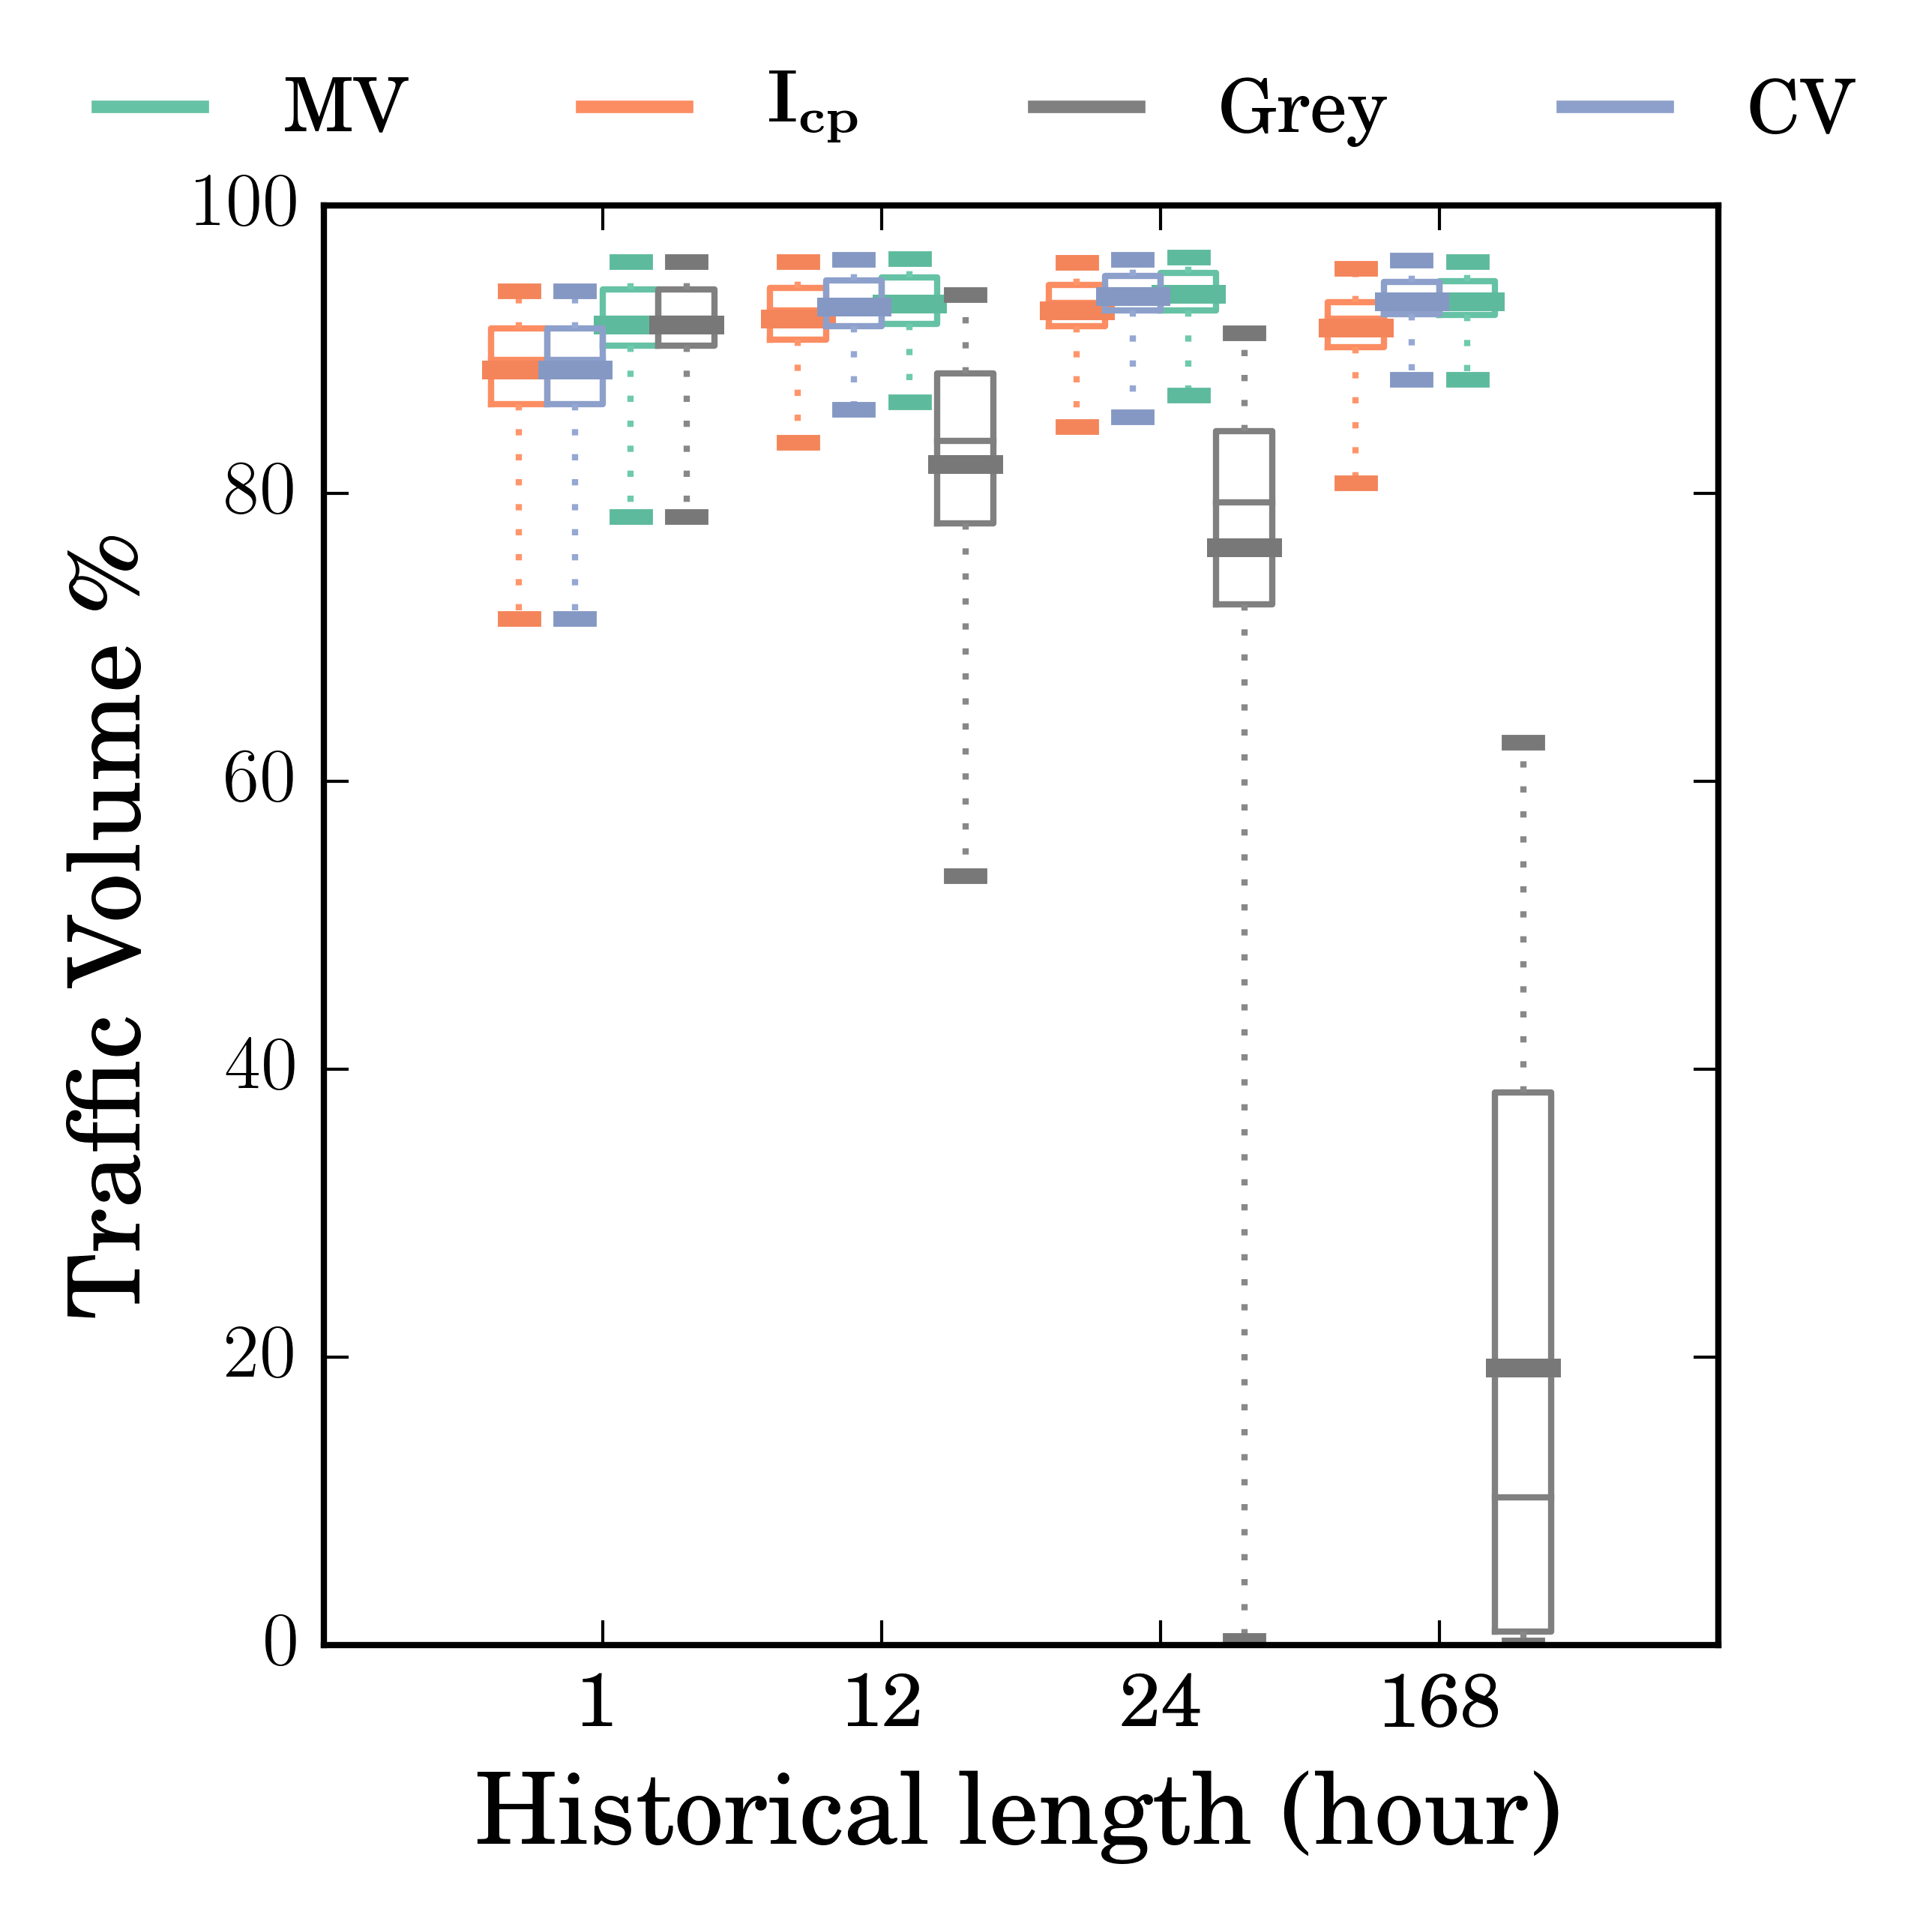
\includegraphics[width=\textwidth]{gfx/chap2/grey_cvg_box_method_compare_fs_sa.png}
                \caption{SA}
                \label{fig:cvg_sa}
        \end{subfigure}
        \begin{subfigure}[b]{0.48\textwidth}
                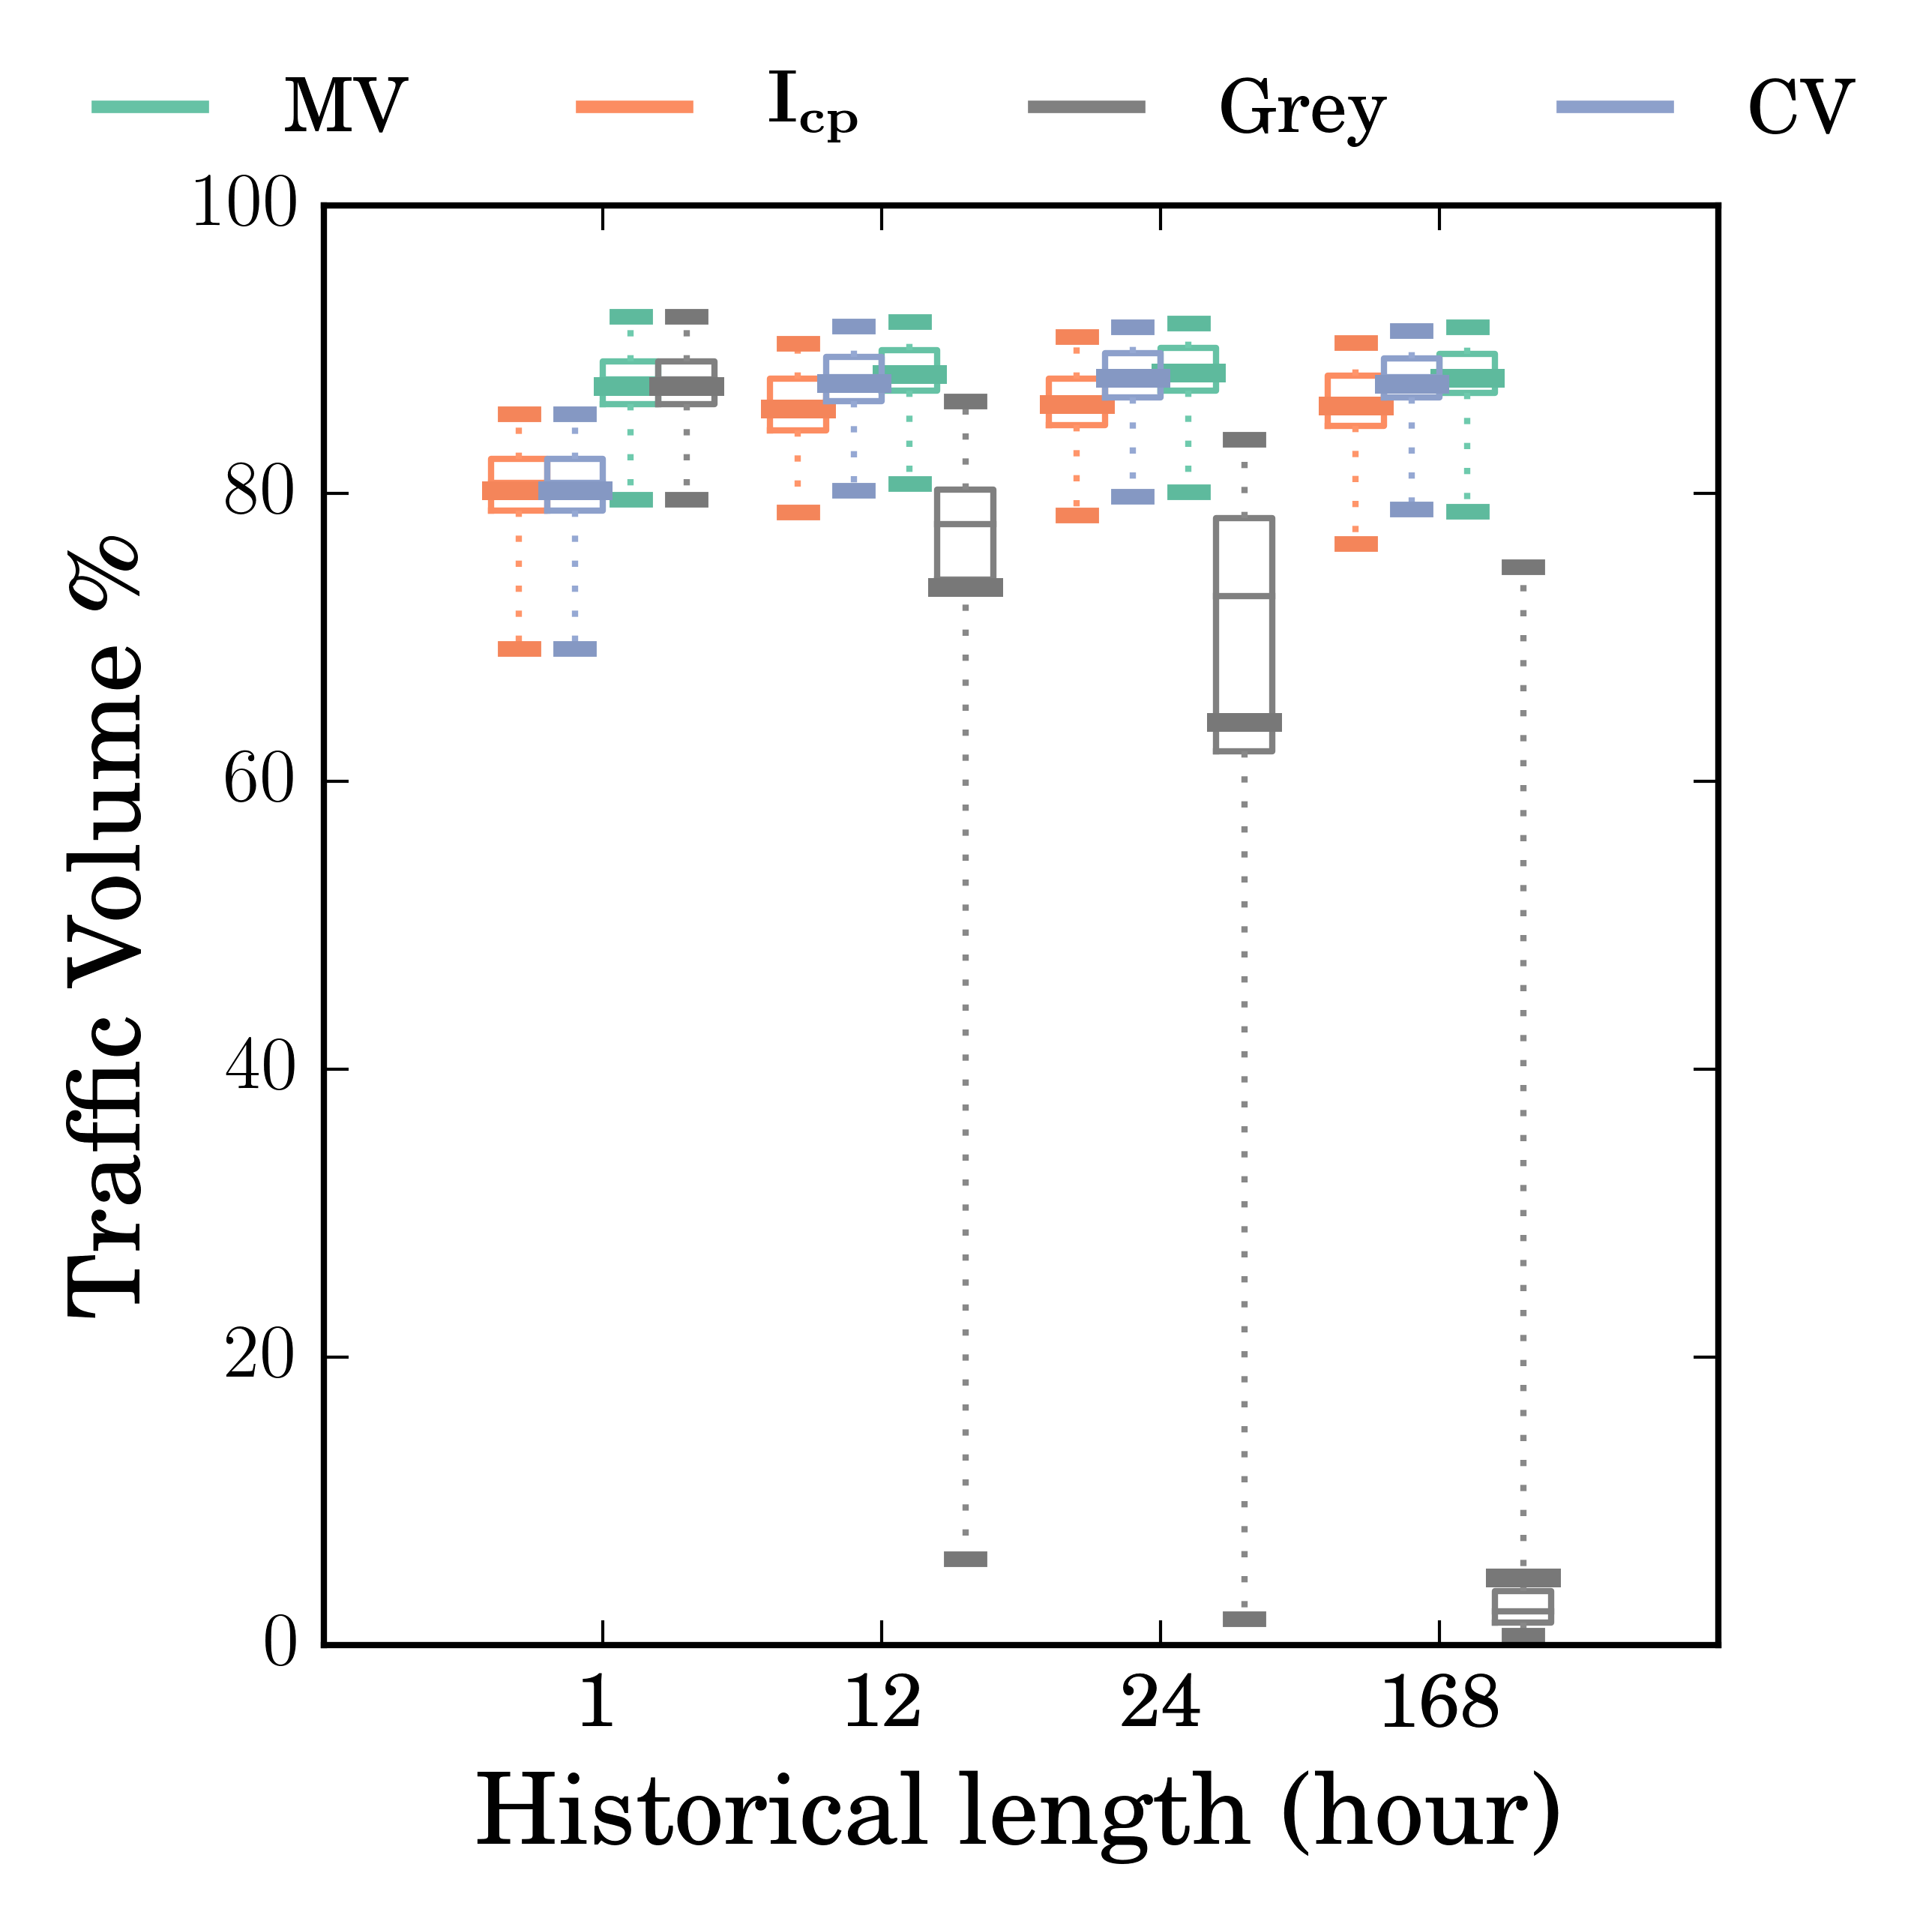
\includegraphics[width=\textwidth]{gfx/chap2/grey_cvg_box_method_compare_fs_sb.png}
                \caption{SB}
                \label{fig:cvg_sb}
        \end{subfigure}
        \begin{subfigure}[b]{0.48\textwidth}
                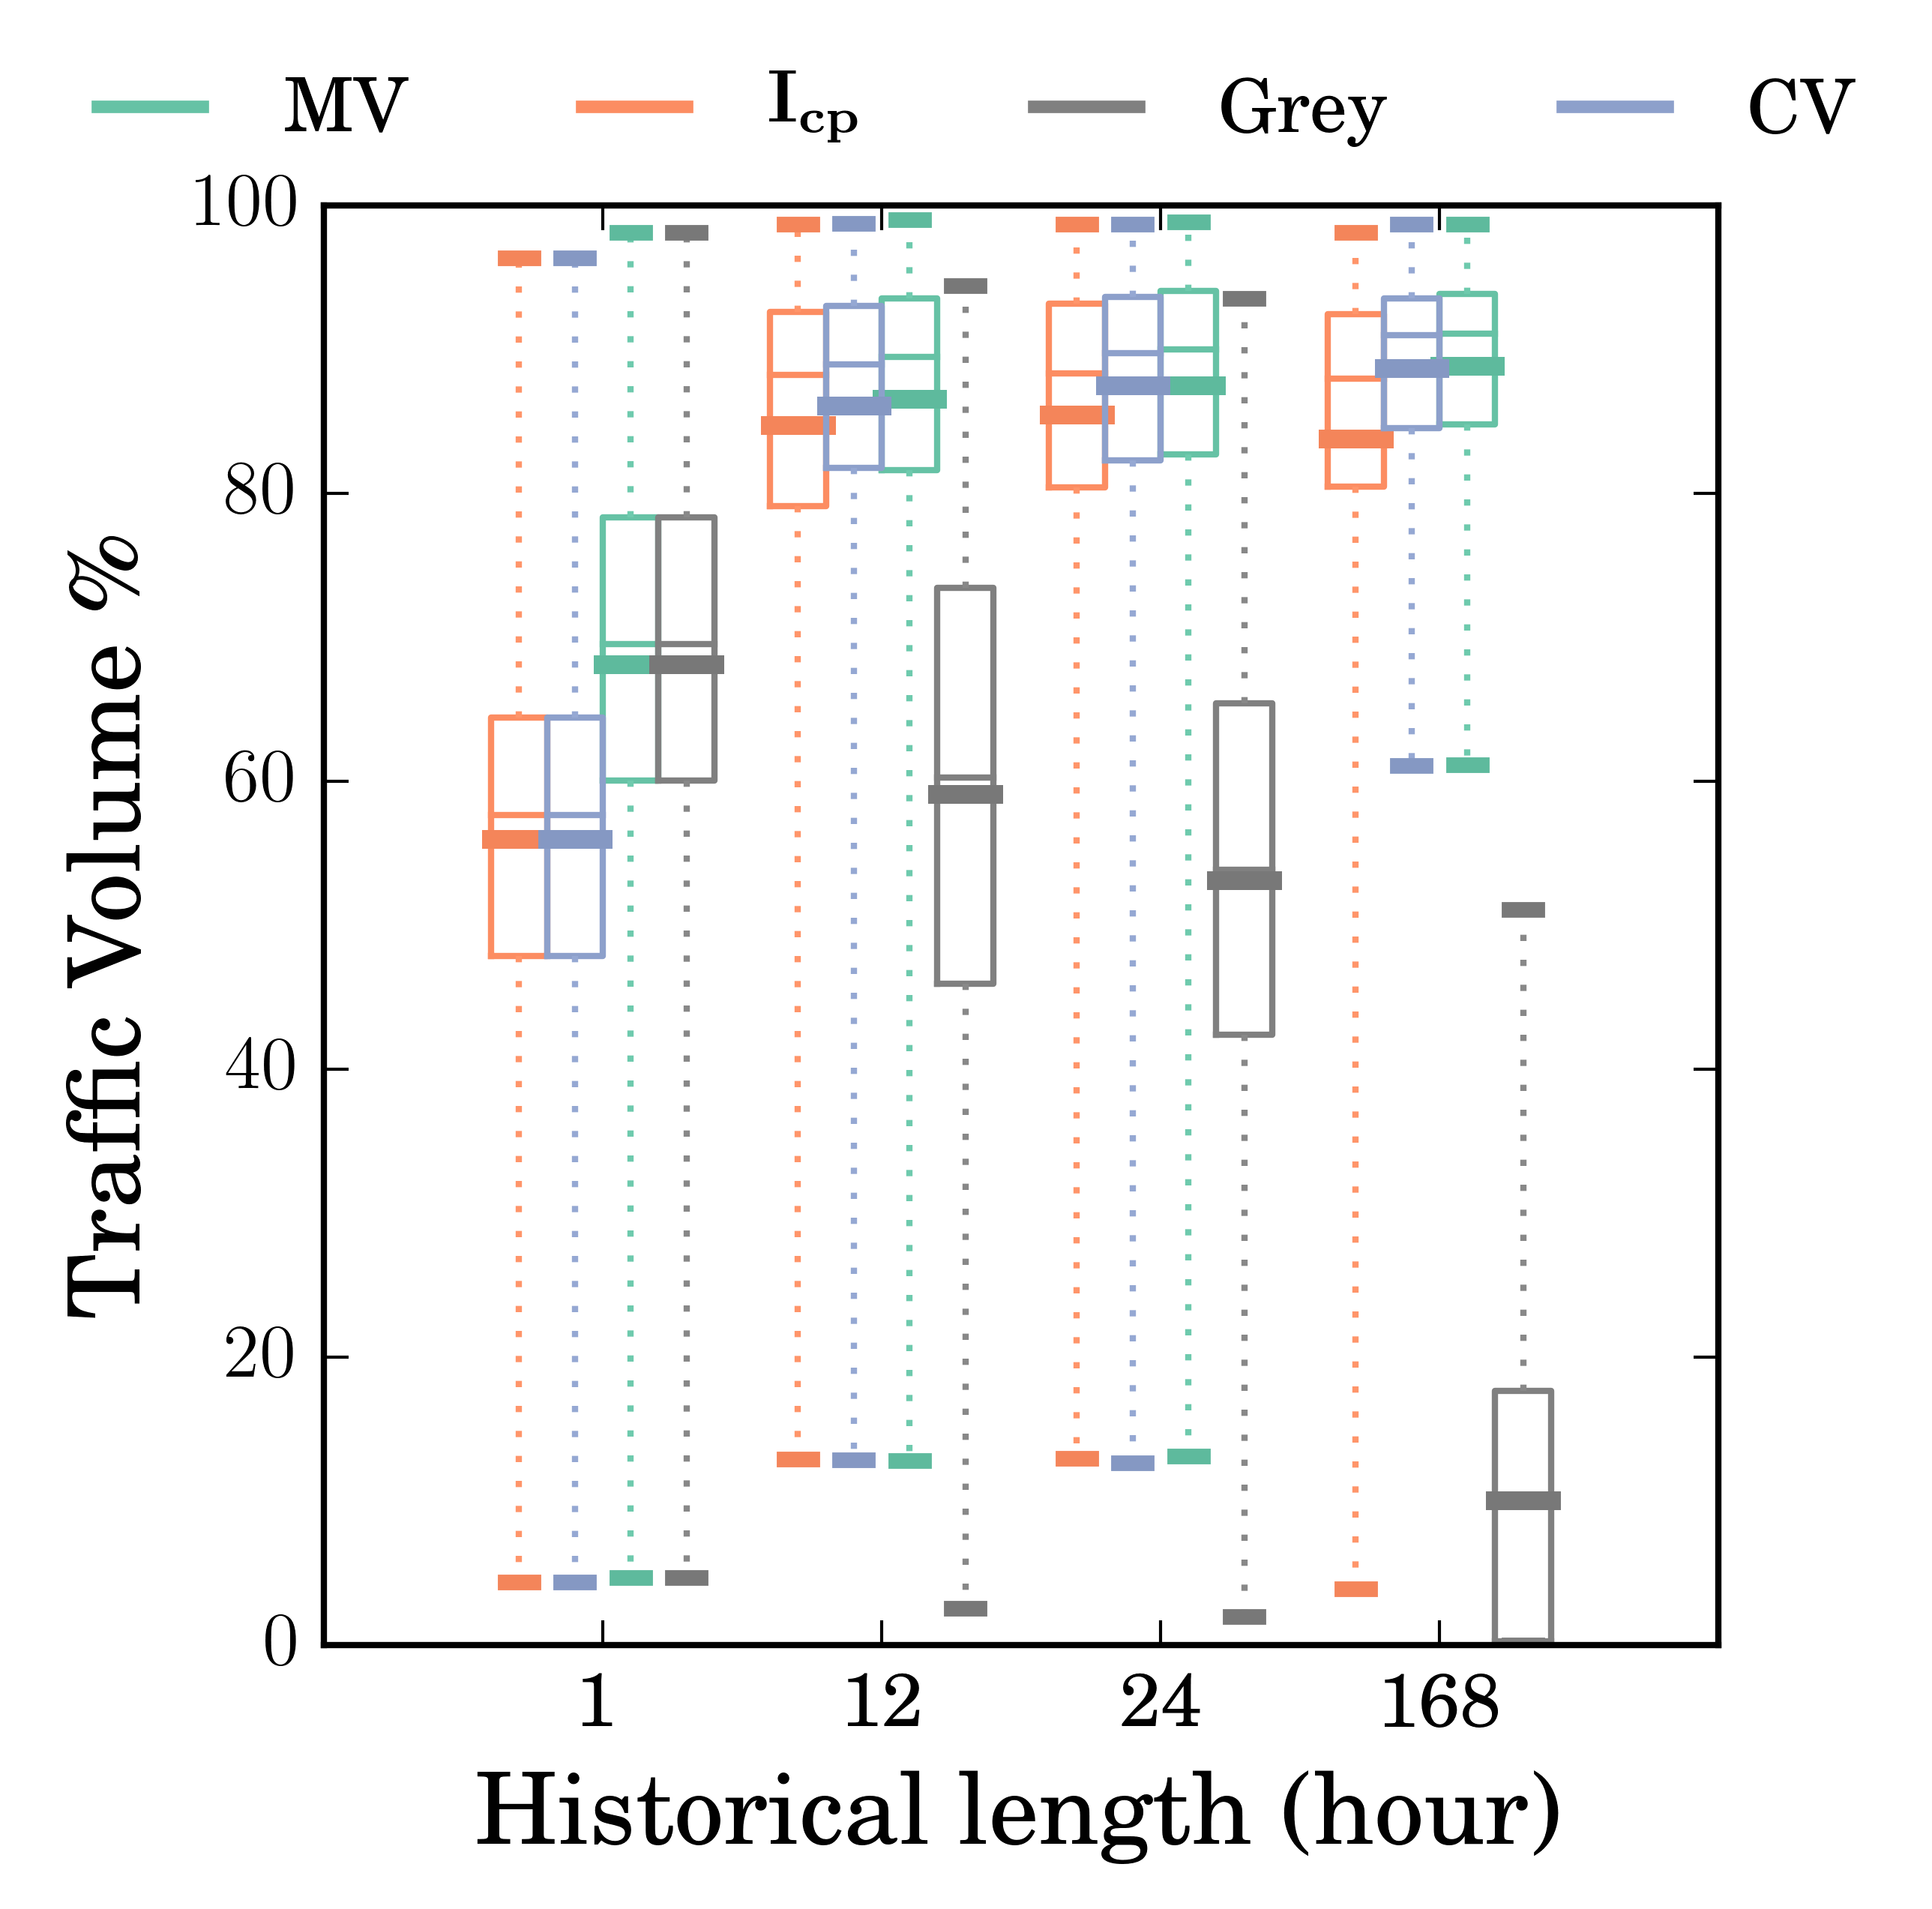
\includegraphics[width=\textwidth]{gfx/chap2/grey_cvg_box_method_compare_fs_sc.png}
                \caption{SC}
                \label{fig:cvg_sc}
        \end{subfigure}
        \begin{subfigure}[b]{0.48\textwidth}
                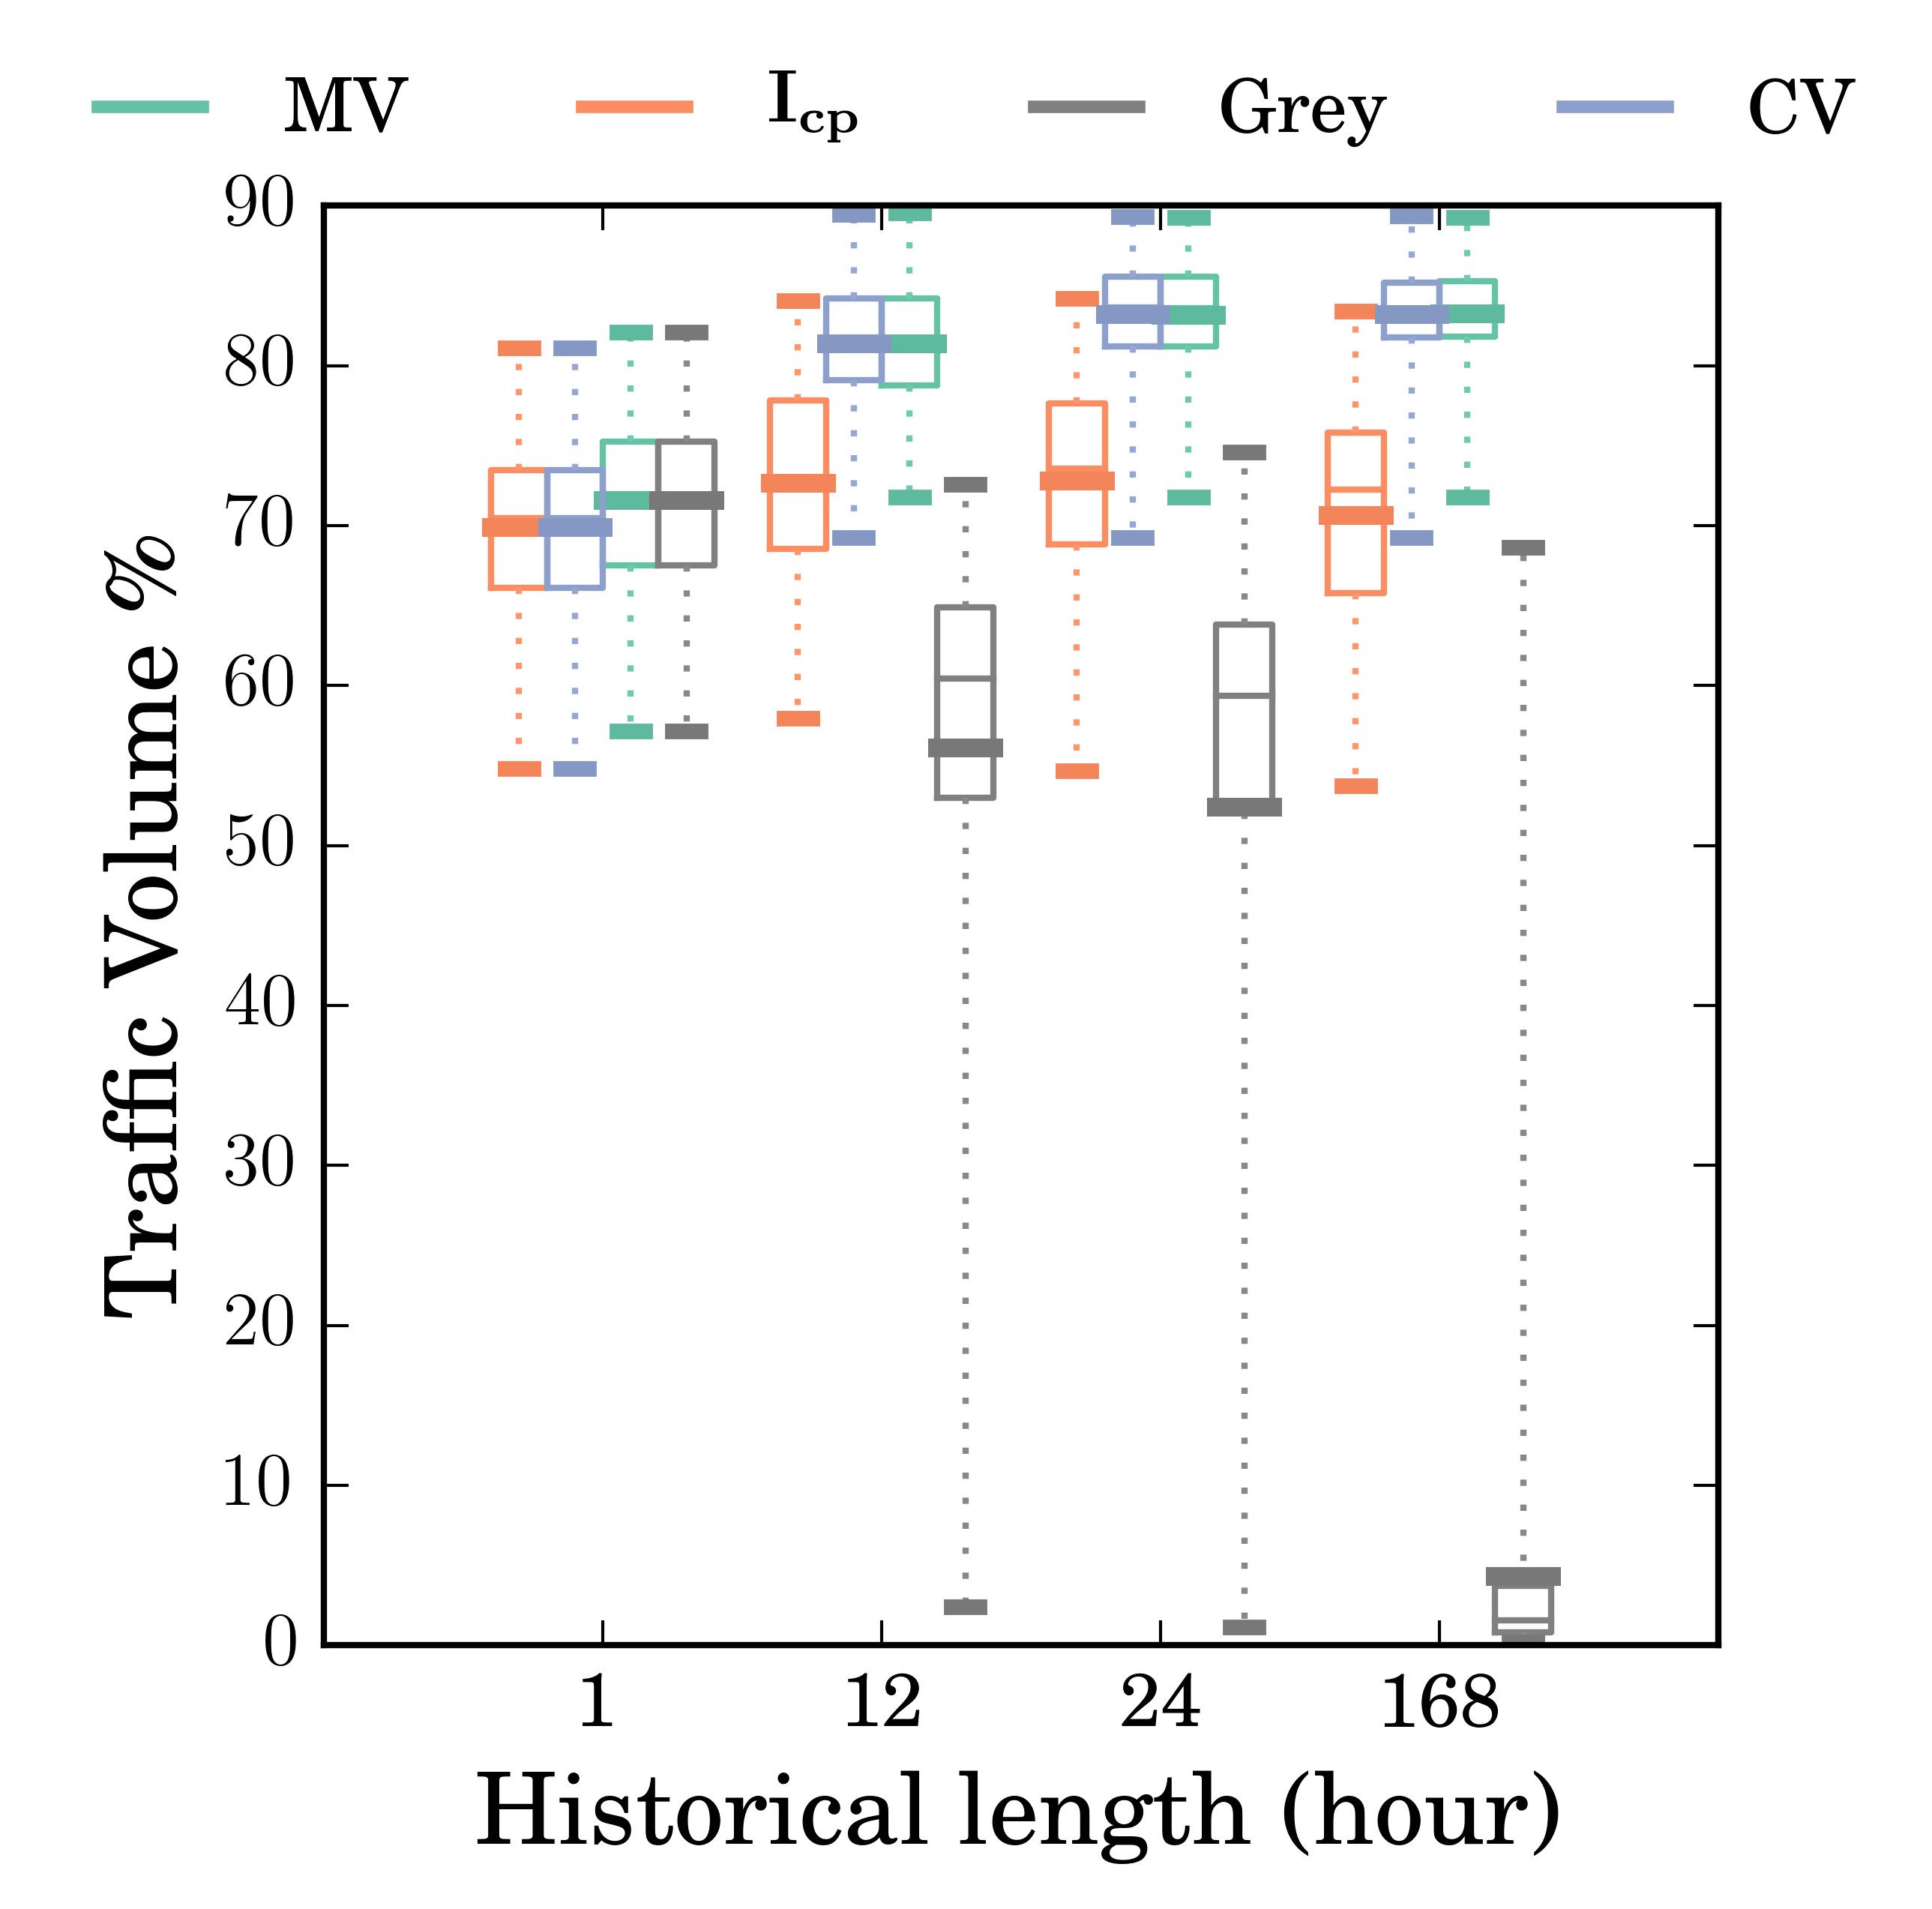
\includegraphics[width=\textwidth]{gfx/chap2/grey_cvg_box_method_compare_fs_sd.png}
                \caption{SD}
                \label{fig:cvg_sd}
        \end{subfigure}
        \begin{subfigure}[b]{0.48\textwidth}
                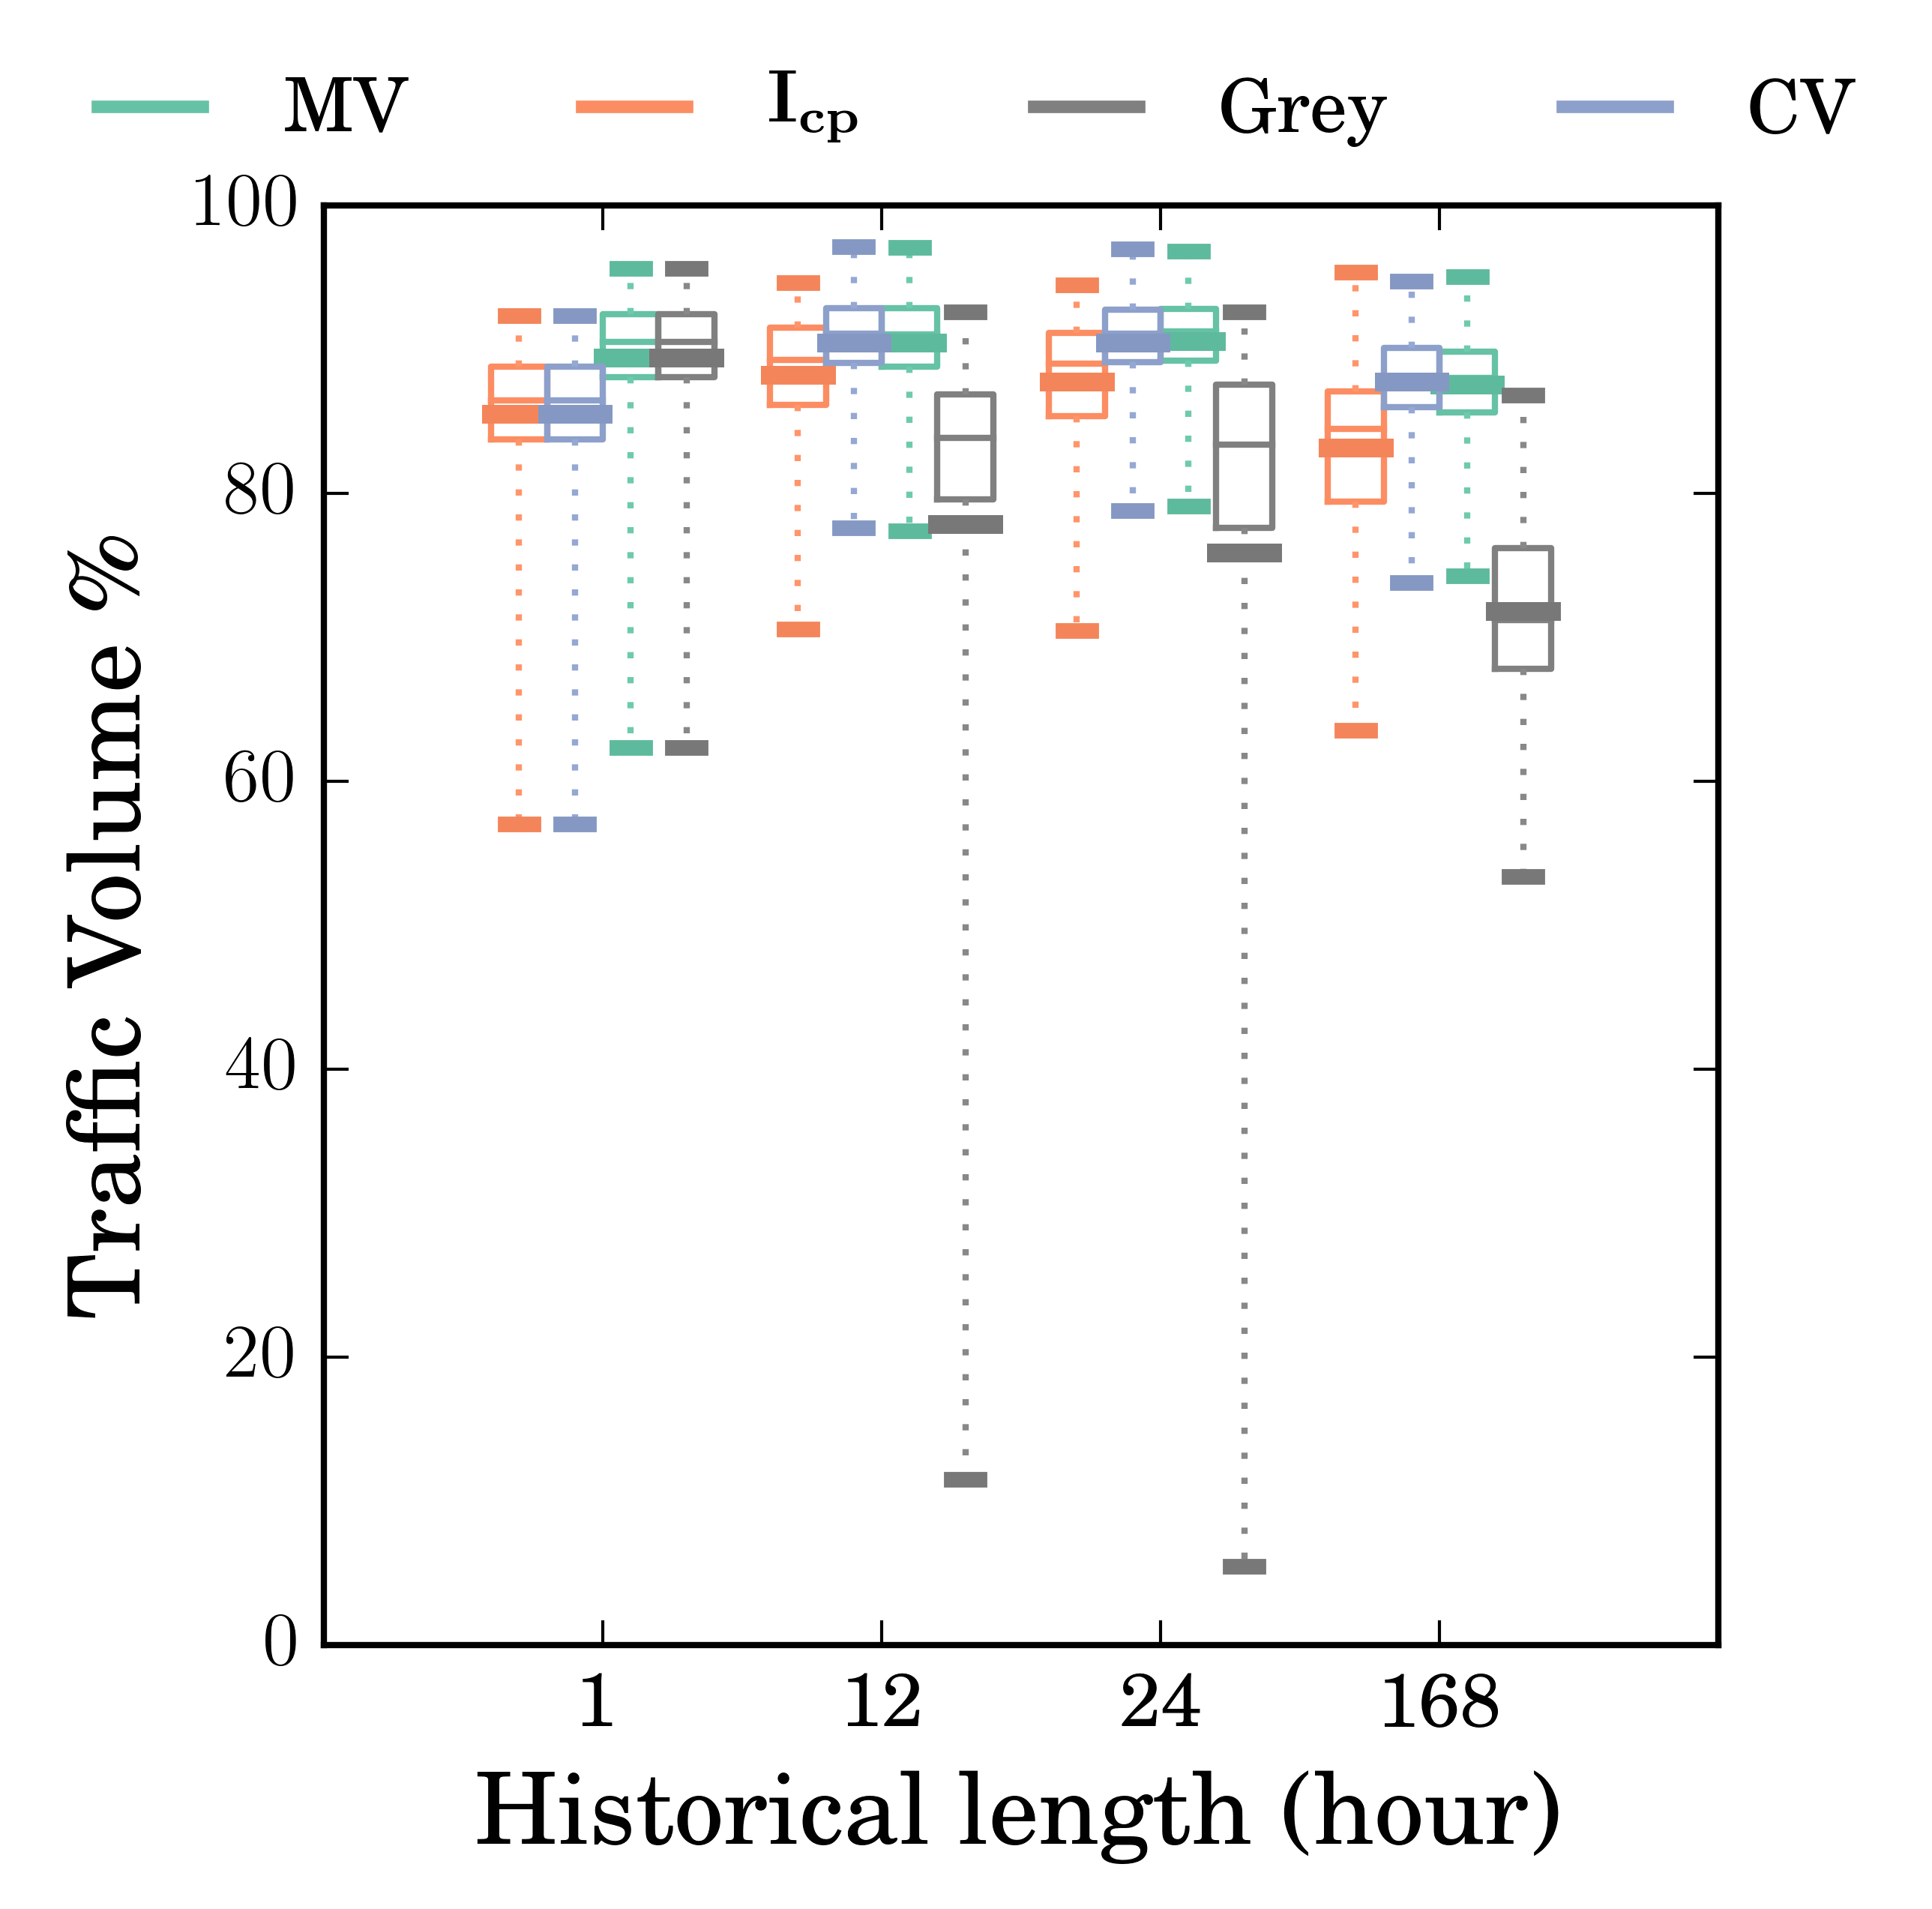
\includegraphics[width=\textwidth]{gfx/chap2/grey_cvg_box_method_compare_fs_se.png}
                \caption{SE}
                \label{fig:cvg_se}
        \end{subfigure}
        \begin{subfigure}[b]{0.48\textwidth}
                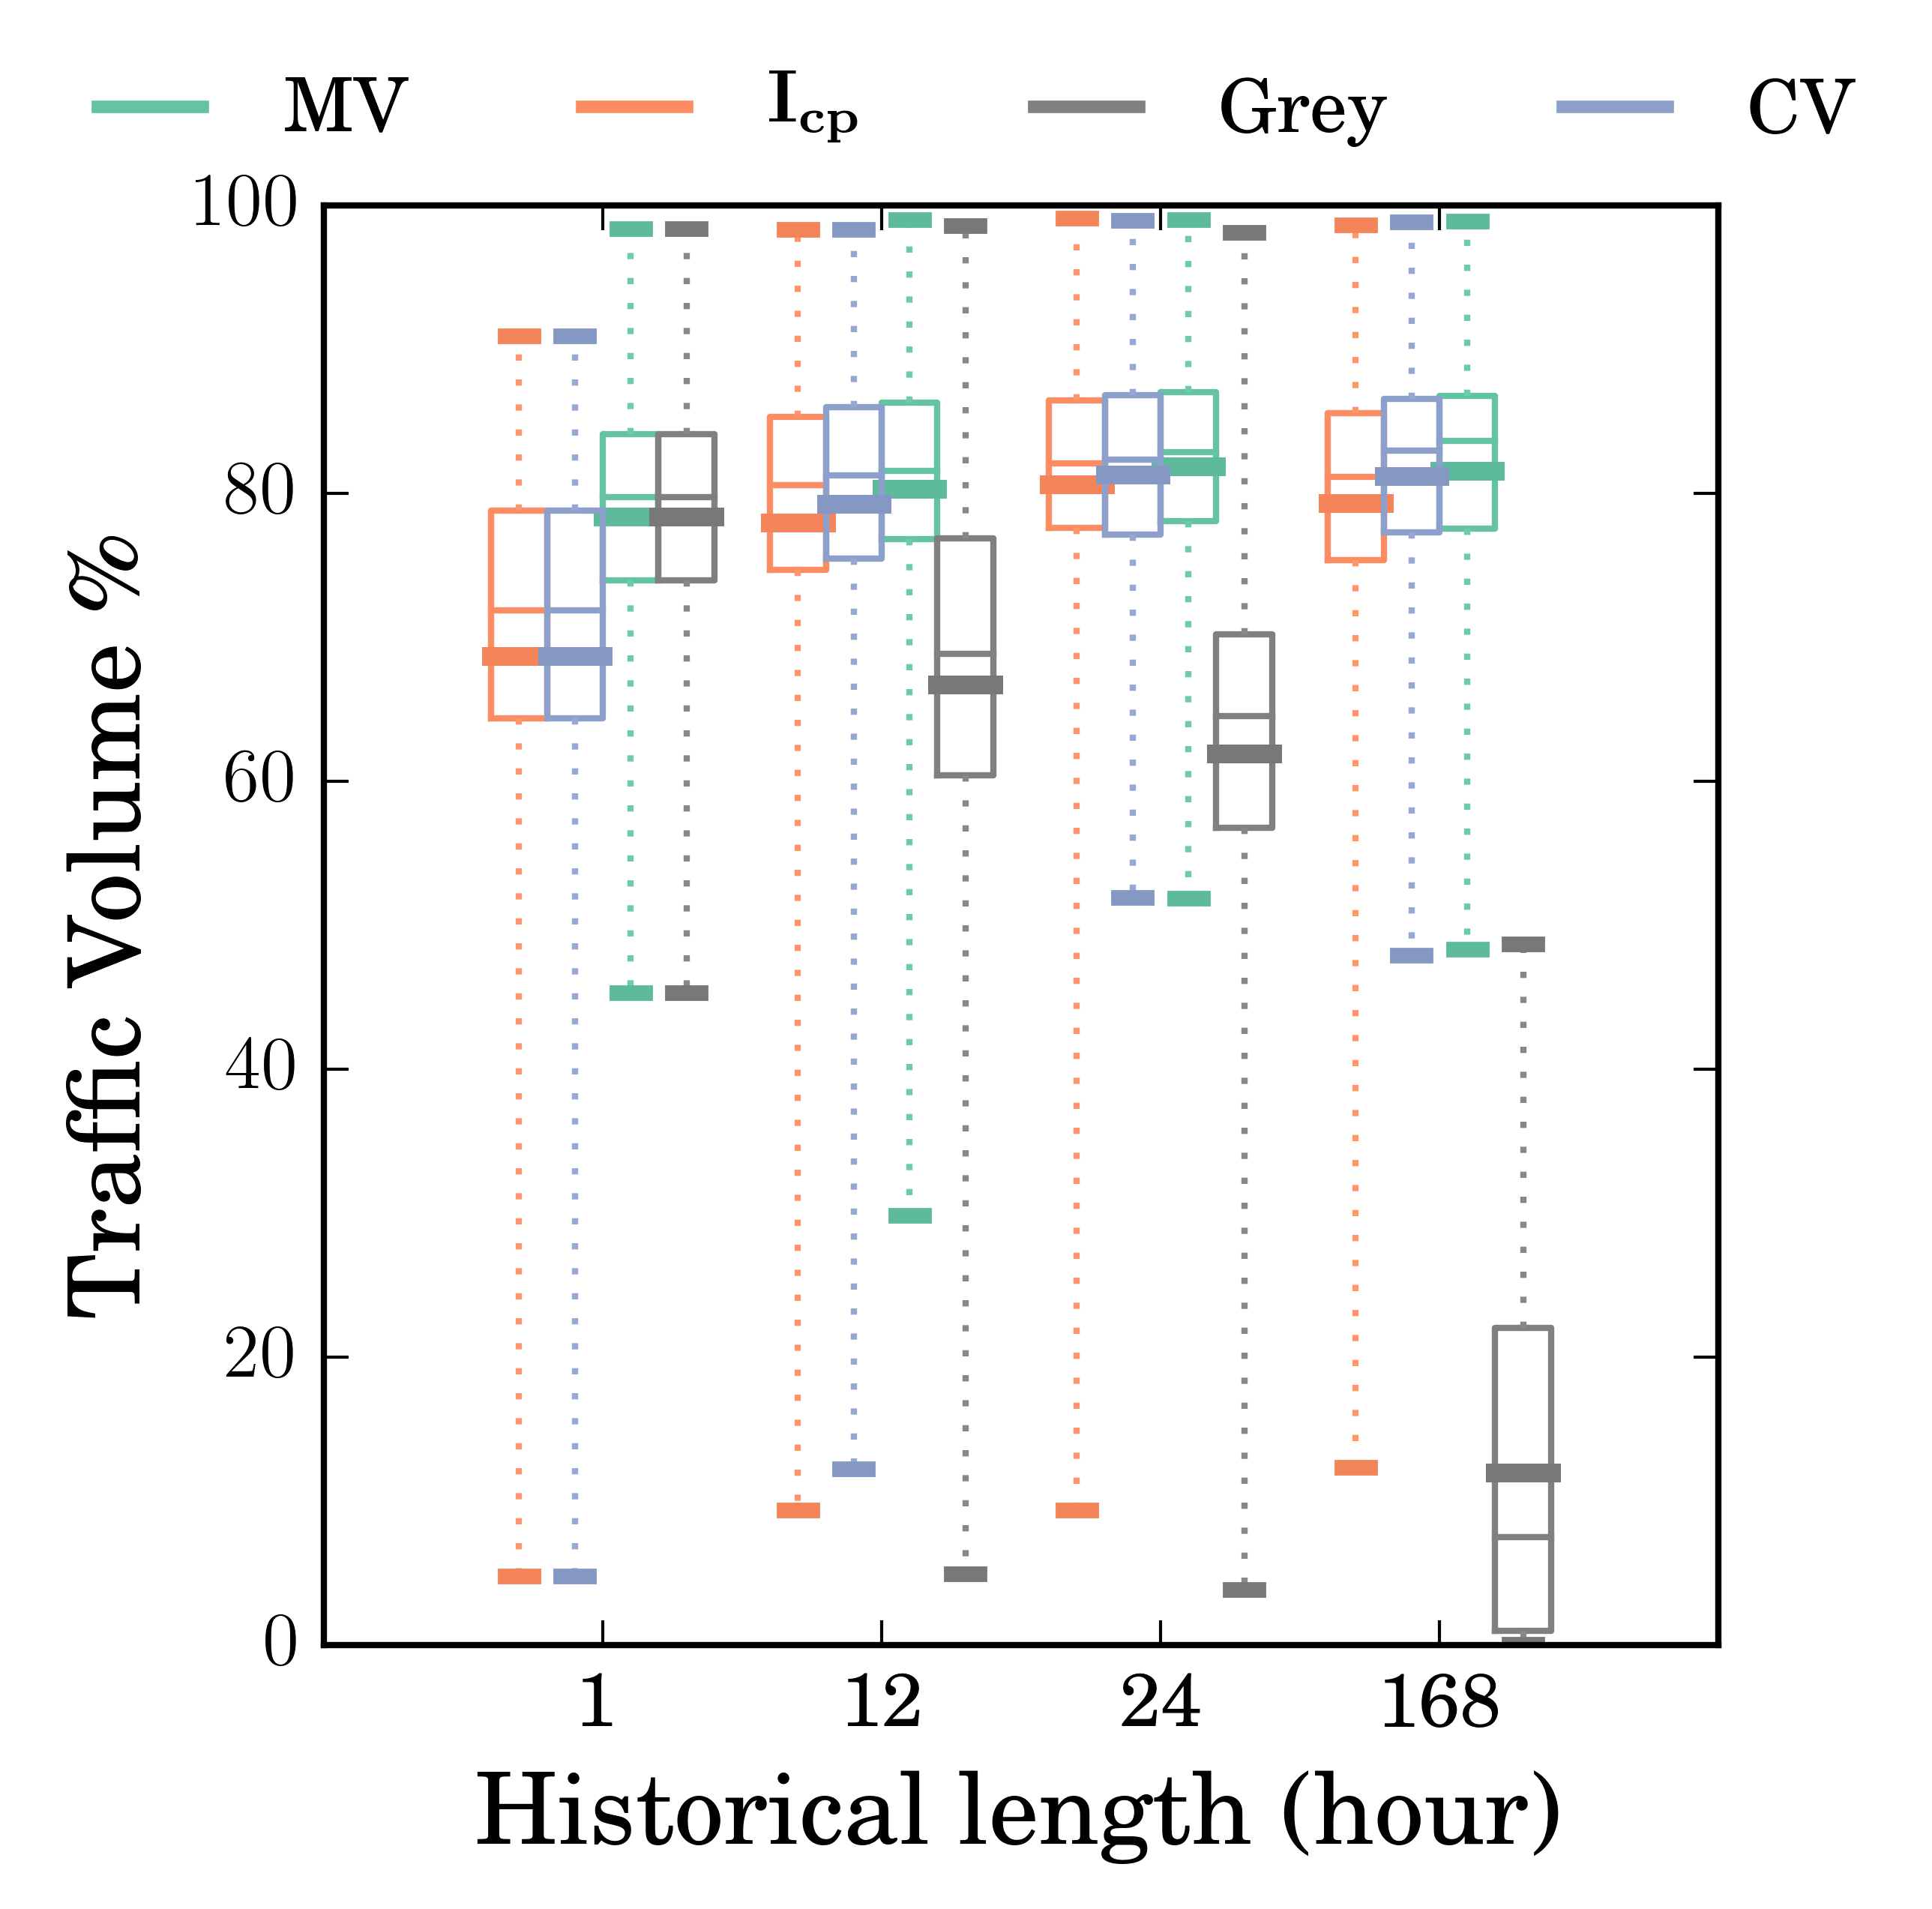
\includegraphics[width=\textwidth]{gfx/chap2/grey_cvg_box_method_compare_fs_sf.png}
                \caption{SF}
                \label{fig:cvg_sf}
        \end{subfigure}
\caption{Hour volume fraction covered by prefixes predictively selected using historical records of different lengths. The selection set size of each network is set to the maximum \textit{core} size over the week starting from June 1st, 2015, see in Table~\ref{tab:core_size}.}
\label{fig:cvg}
\end{figure}

\begin{figure}\ContinuedFloat
	\centering
        \begin{subfigure}[b]{0.48\textwidth}
                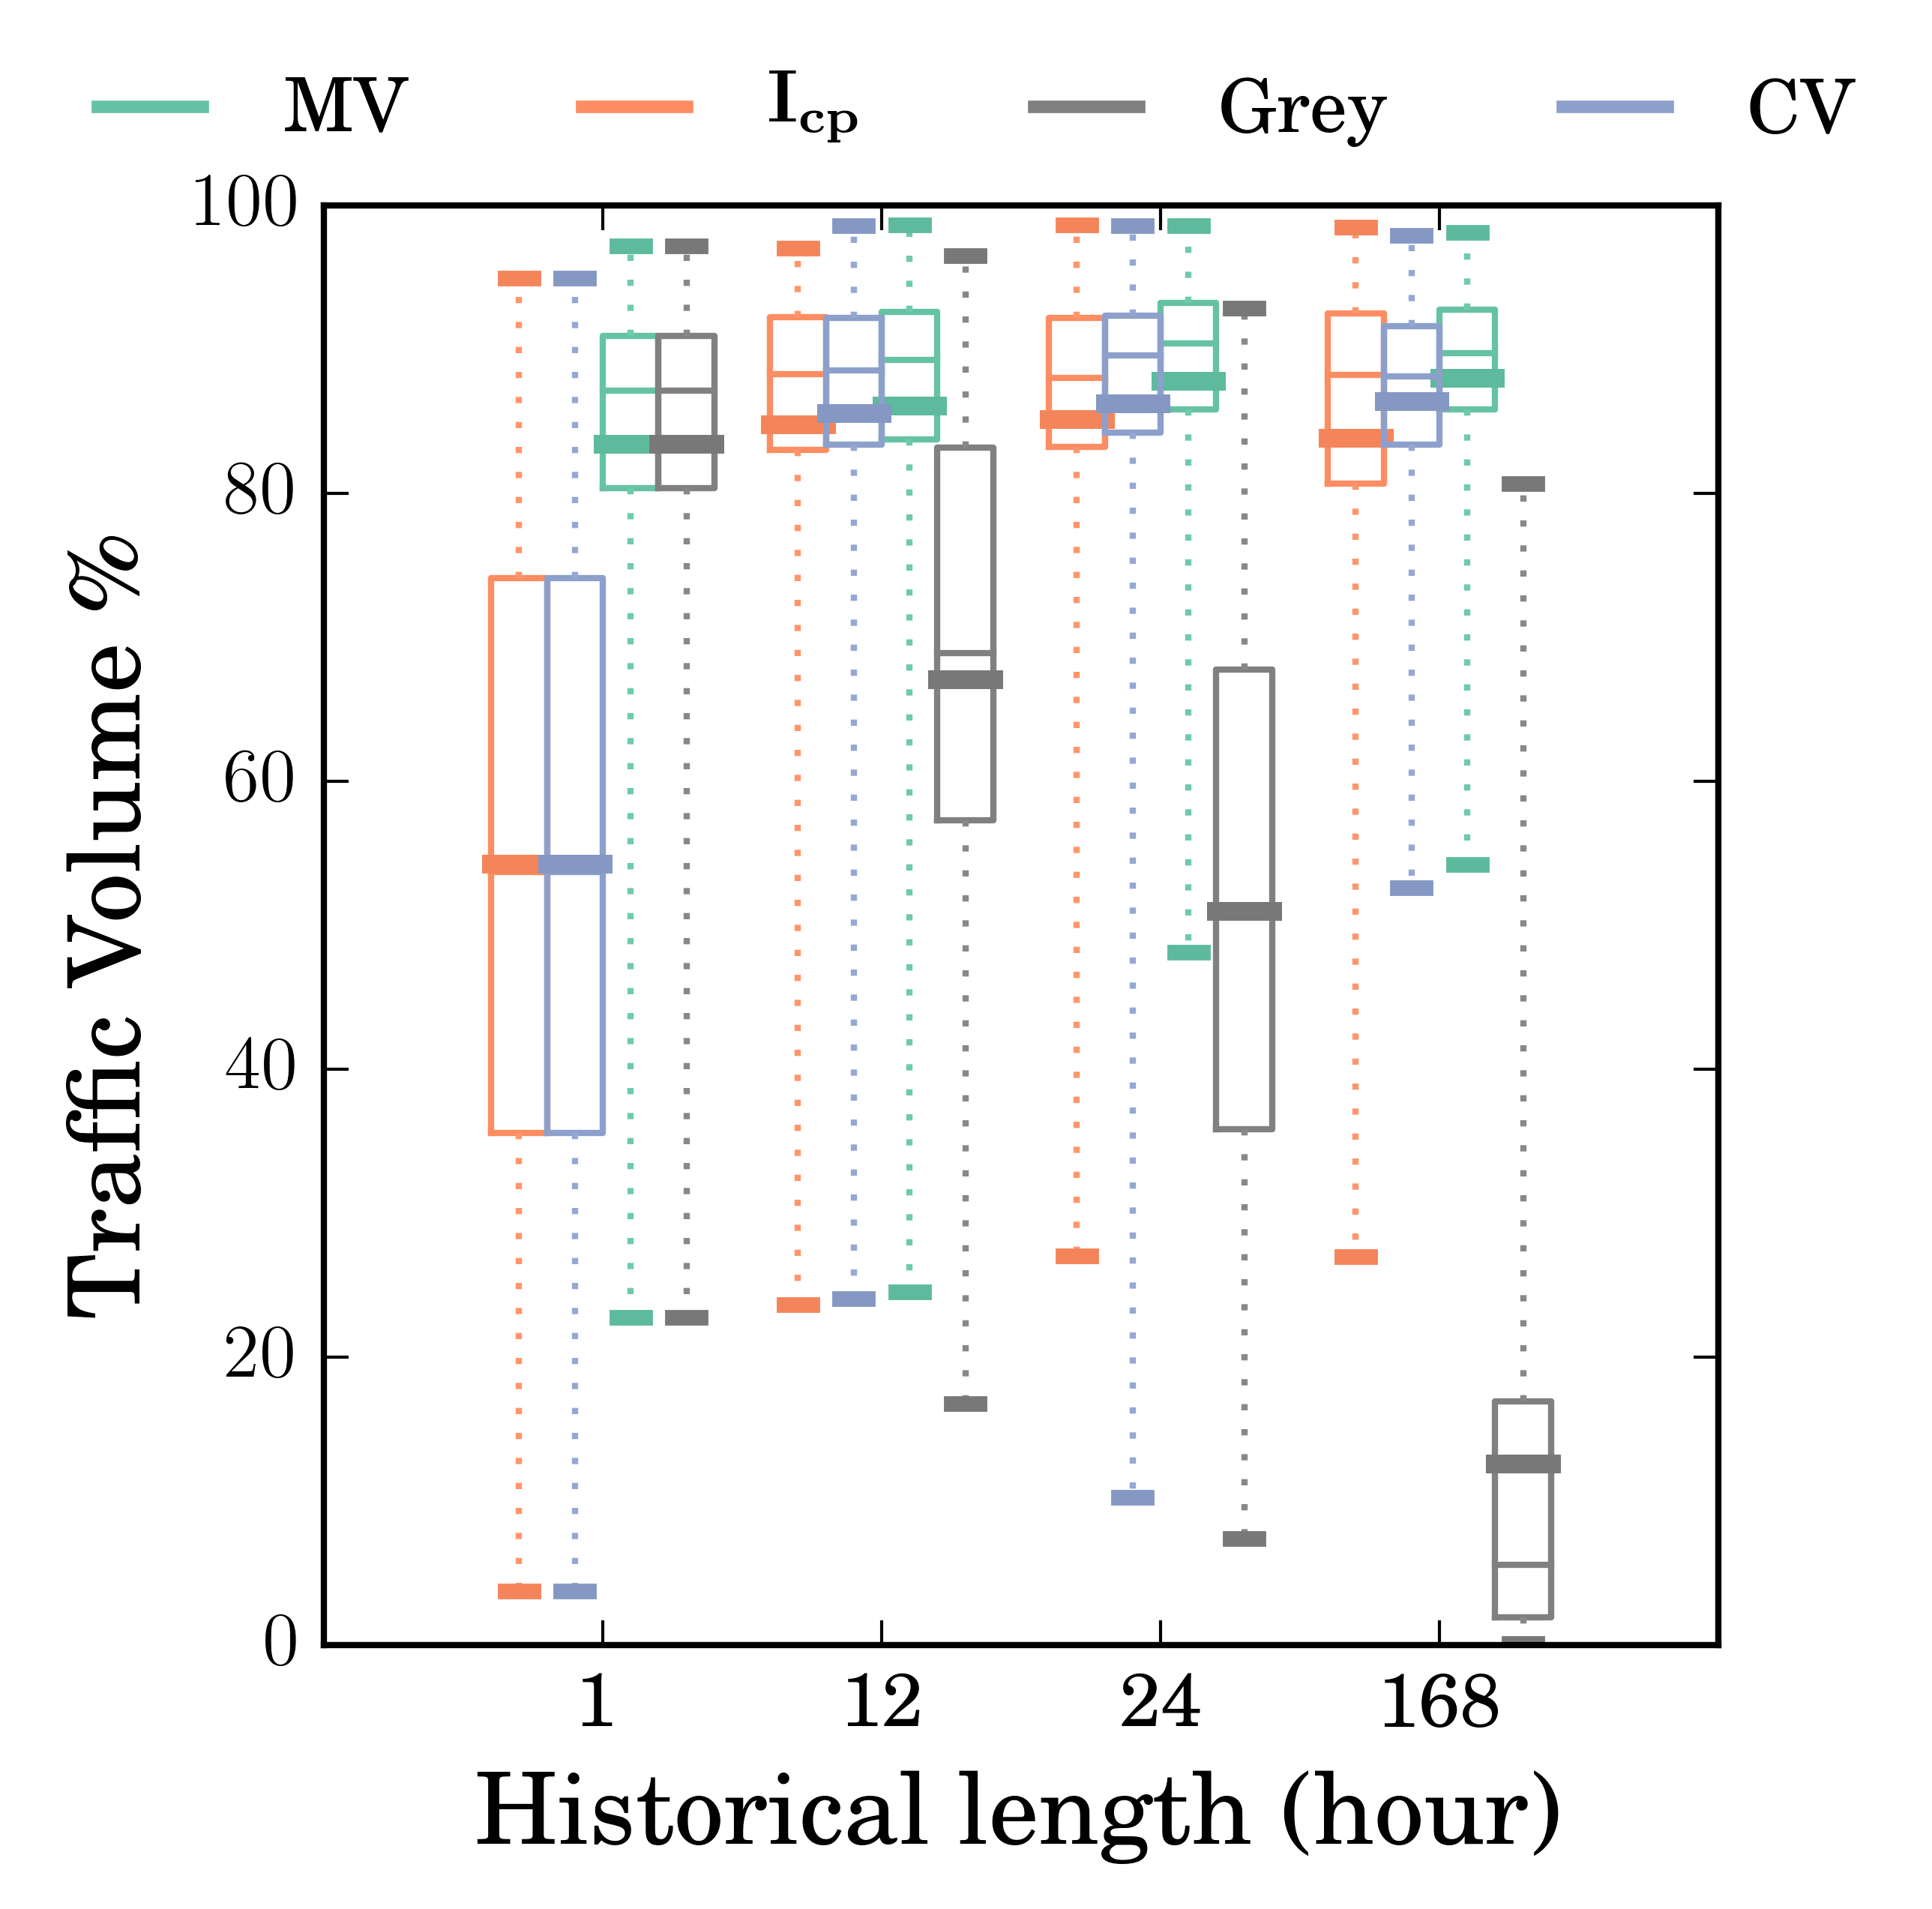
\includegraphics[width=\textwidth]{gfx/chap2/grey_cvg_box_method_compare_fs_sg.png}
                \caption{SG}
                \label{fig:cvg_sg}
        \end{subfigure}
        \begin{subfigure}[b]{0.48\textwidth}
                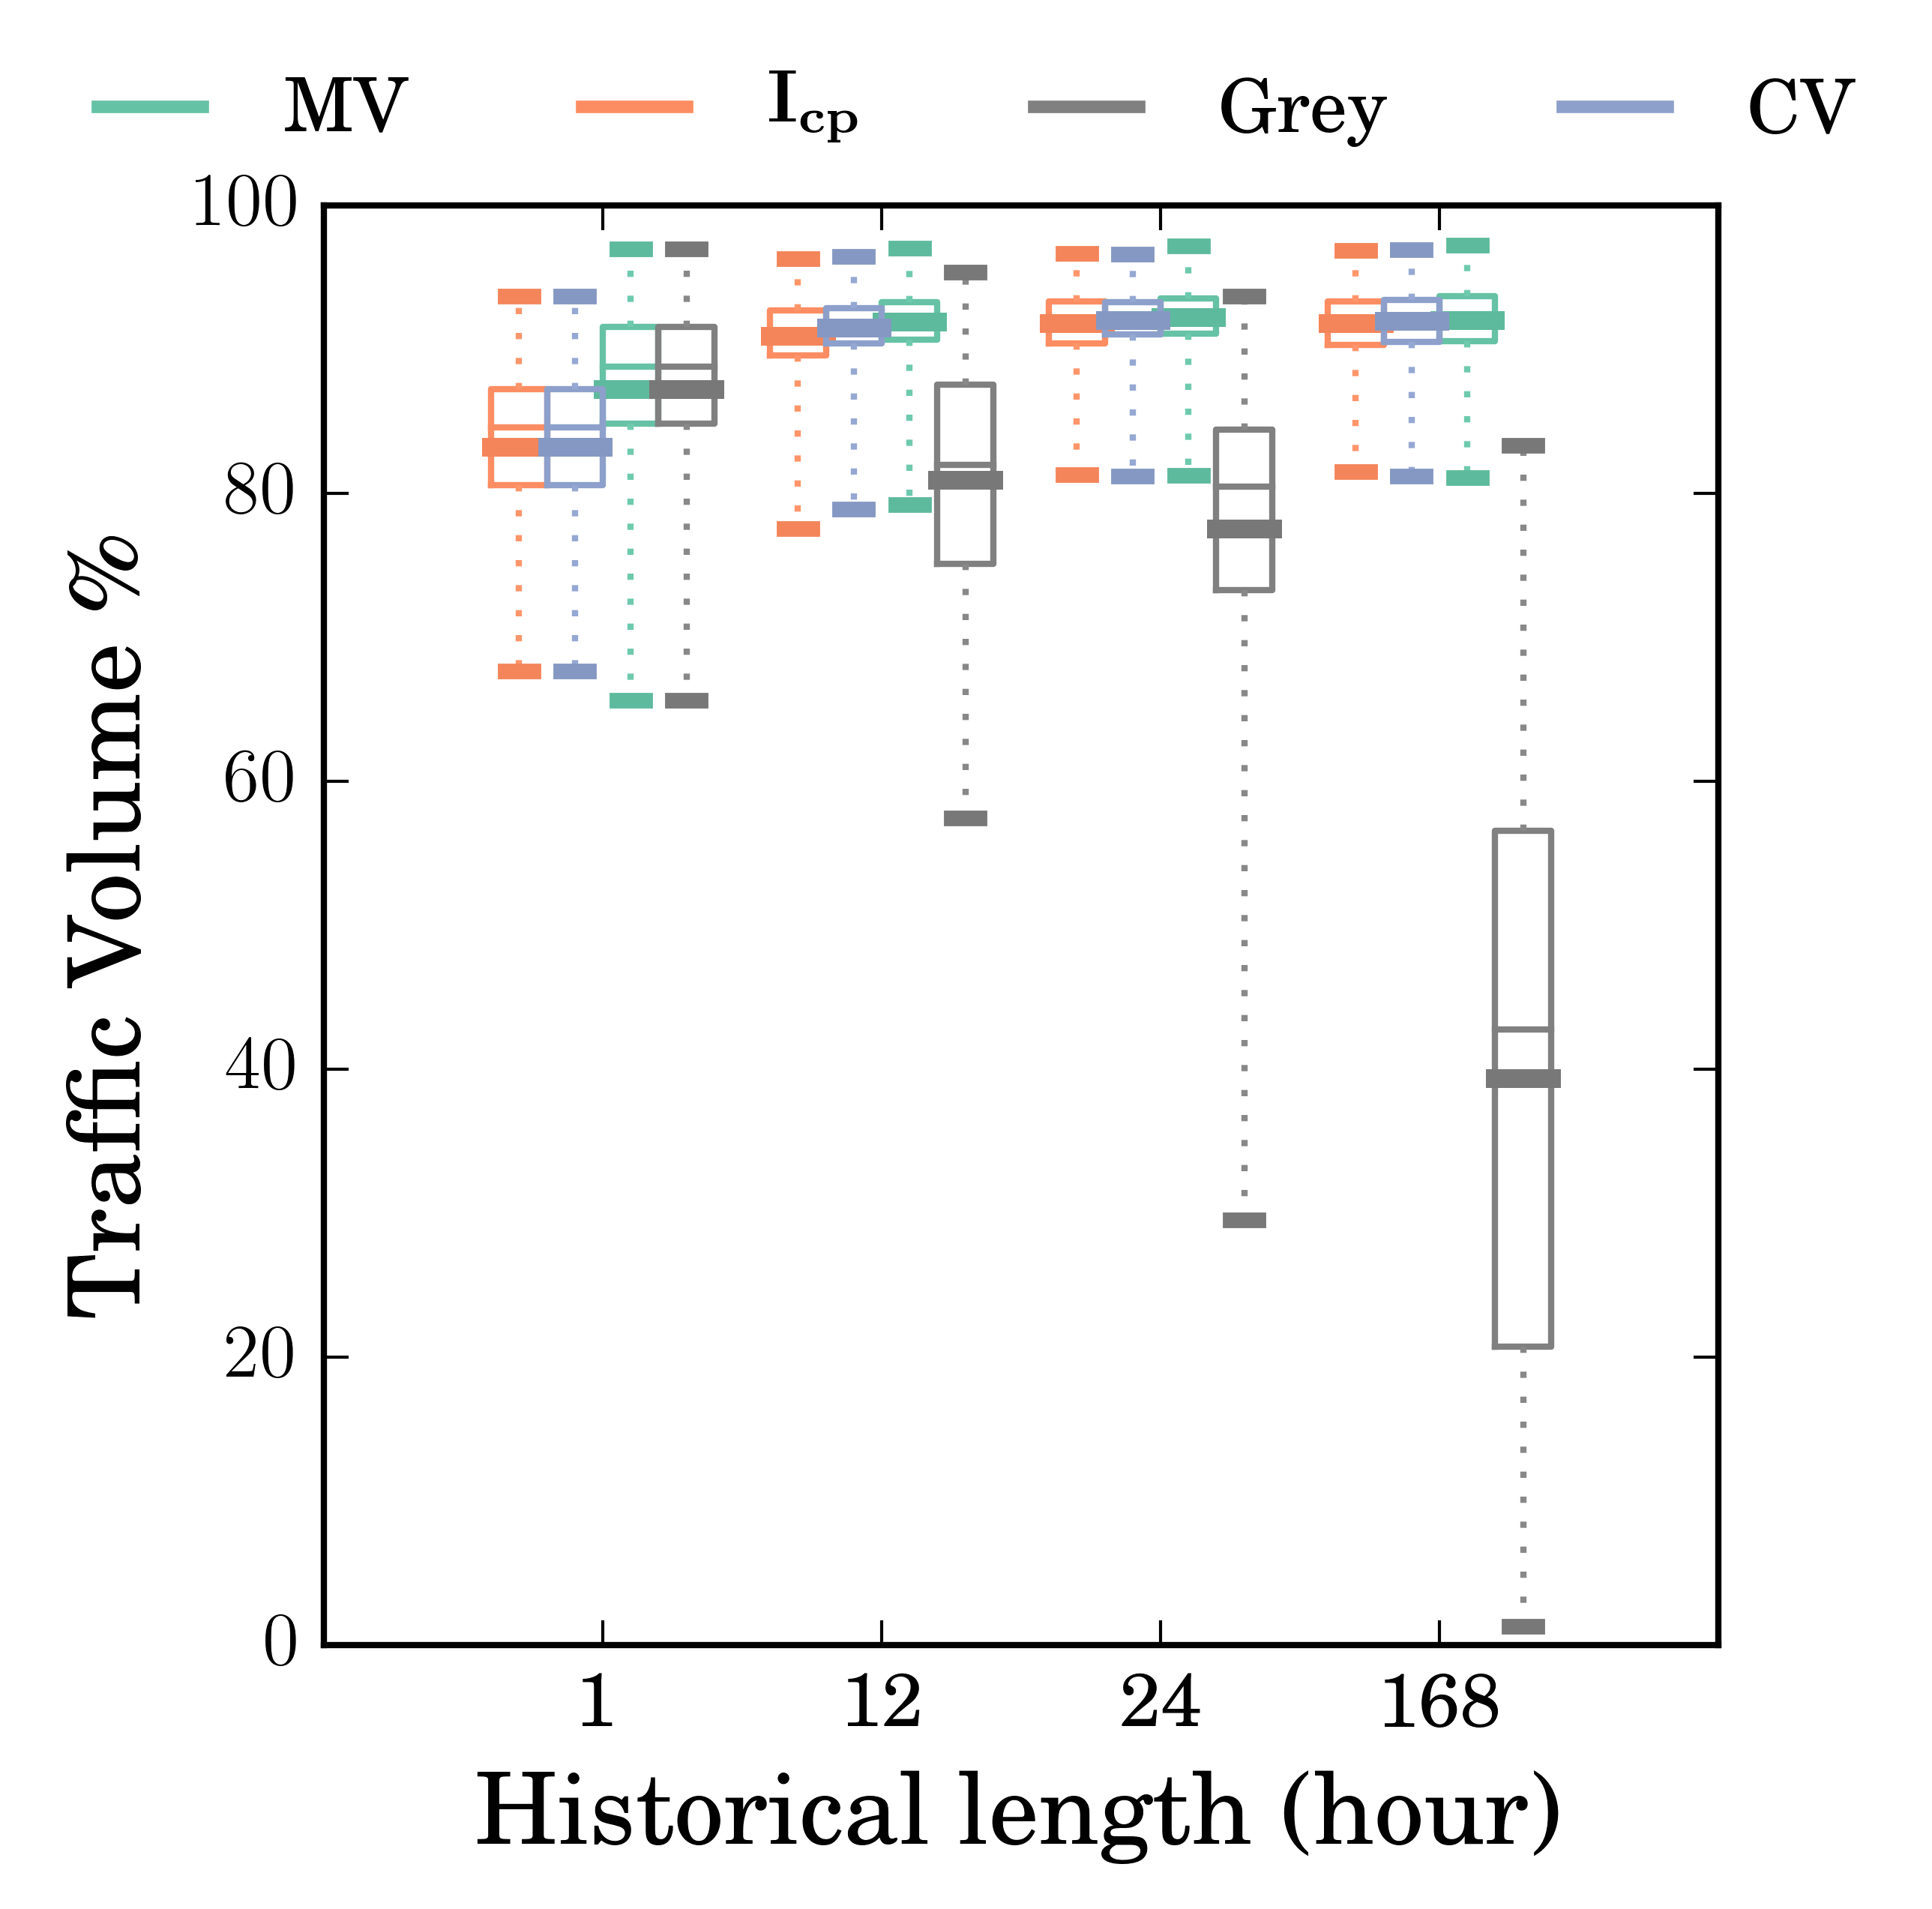
\includegraphics[width=\textwidth]{gfx/chap2/grey_cvg_box_method_compare_fs_sh.png}
                \caption{SH}
                \label{fig:cvg_sh}
        \end{subfigure}
        \begin{subfigure}[b]{0.48\textwidth}
                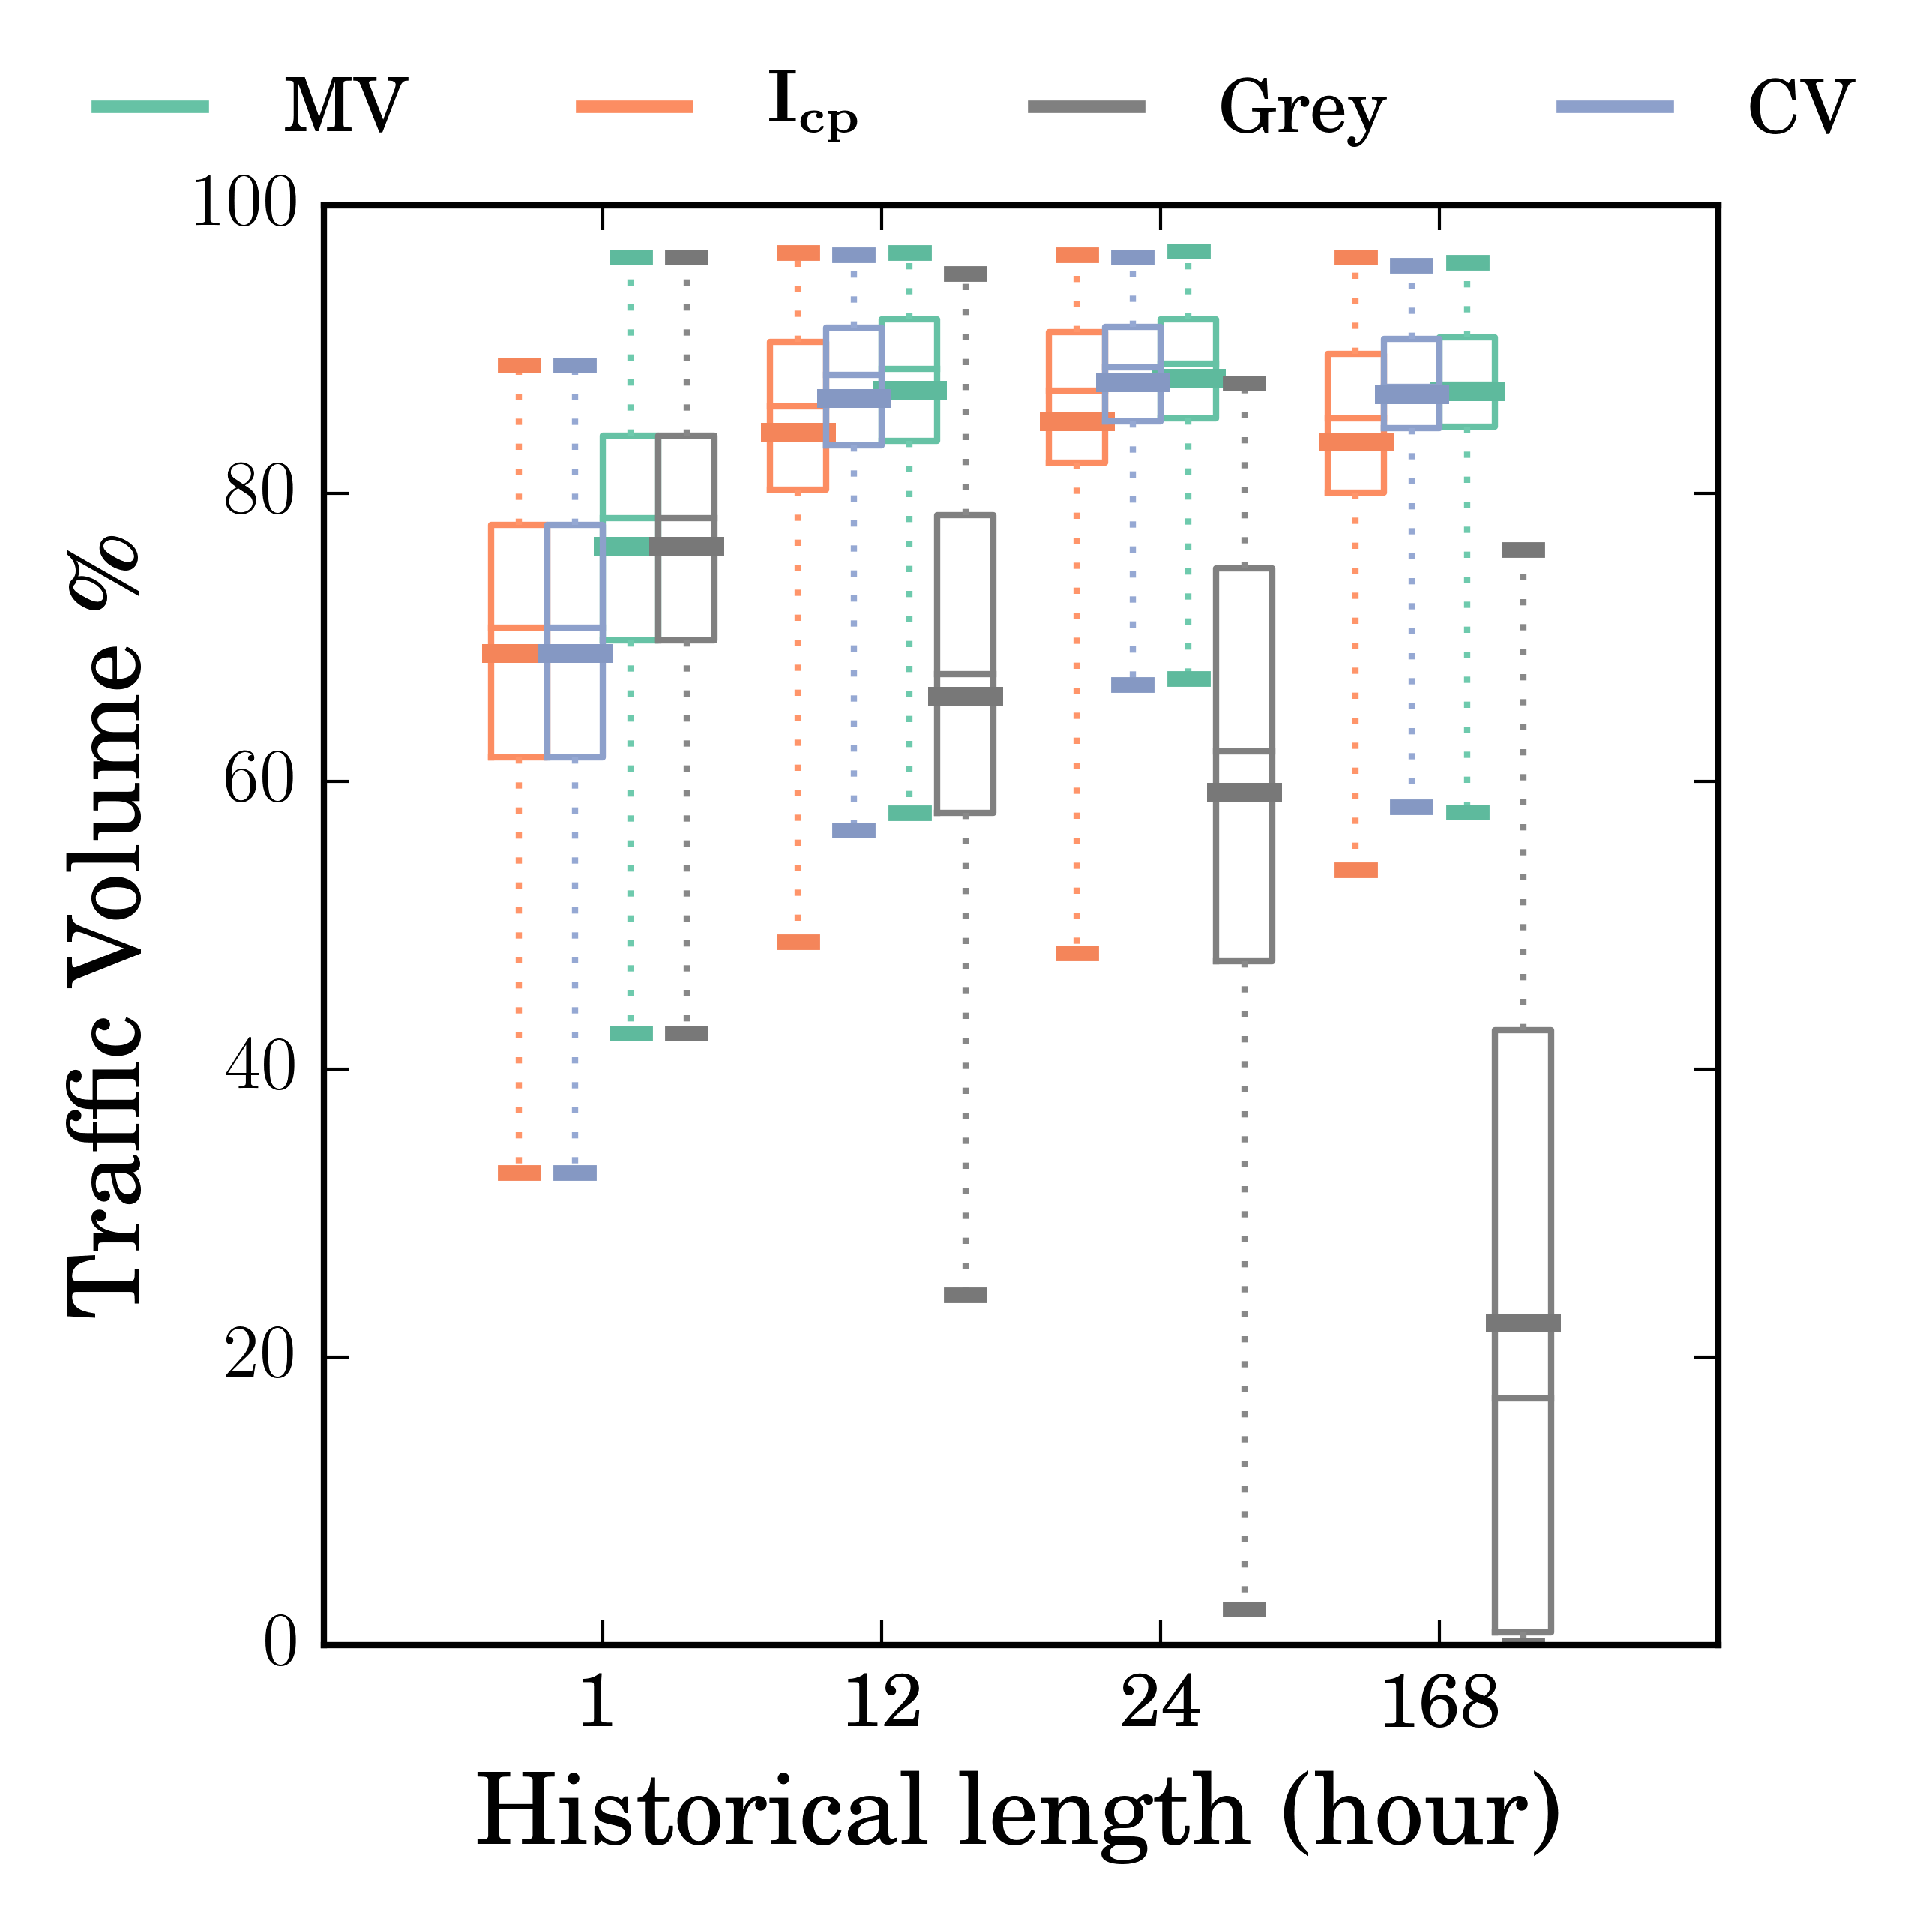
\includegraphics[width=\textwidth]{gfx/chap2/grey_cvg_box_method_compare_fs_si.png}
                \caption{SI}
                \label{fig:cvg_si}
        \end{subfigure}
\caption{(cont.) Hour volume fraction covered by prefixes predictively selected using historical records of different lengths.}
\label{fig:cvg_cont}
\end{figure}

%\marginpar{volume coverage}
In evaluating and comparing the performance of these methods, we fixed the selection set size to the maximum \textit{core} size over the week. 
Figure~\ref{fig:cvg} illustrates the hour volume coverage by the four methods in the form of box-plot, representing the minimum, maximum, 25th and 75th percentile, medium and mean values (thicker bar in the middle of the box). 
Among proposed metrics, we find that the $CV$ is very close to $MV$ in terms of volume coverage, proving that it is a good approximation of the later.

Basing solely on the last 1 hour records, all methods yield already a mean volume coverage $>80\%$ on SA, SB, SE and SH, which implies a strong continuity in prefix volumes between two consecutive hours. 
On SC and SG, however, using records of last 168 hours, i.e. a week, offers much better minimum volume coverage than shorter records. This is due to the fact that at certain hour, SC and SG undergo a great amount of bursty traffic (as observed previously, e.g. in Table~\ref{tab:bi} and Figure~\ref{fig:cv_cp}). By increasing the historical length, the selection metrics are able to have better visibility into the past and capture some of these bursty prefixes --- finally improving the minimum coverage.
The gain in minimum volume coverage by using long historical records can actually be observed on all networks, between 1 hour and 12 hours, also between 12 hour and 24 hour. 
However from 24 hour to 168, this gain doesn't necessary happen on all sites, which is due to the fact that the total volume brought by some highly bursty prefix is diluted by the long time span using $MV$ and $CV$ metrics. In order to capture them, a larger selection set size is need, which inevitably includes more prefixes of few significance.


\begin{figure}
\centering
		\centering
		\begin{subfigure}[b]{0.9\textwidth}
                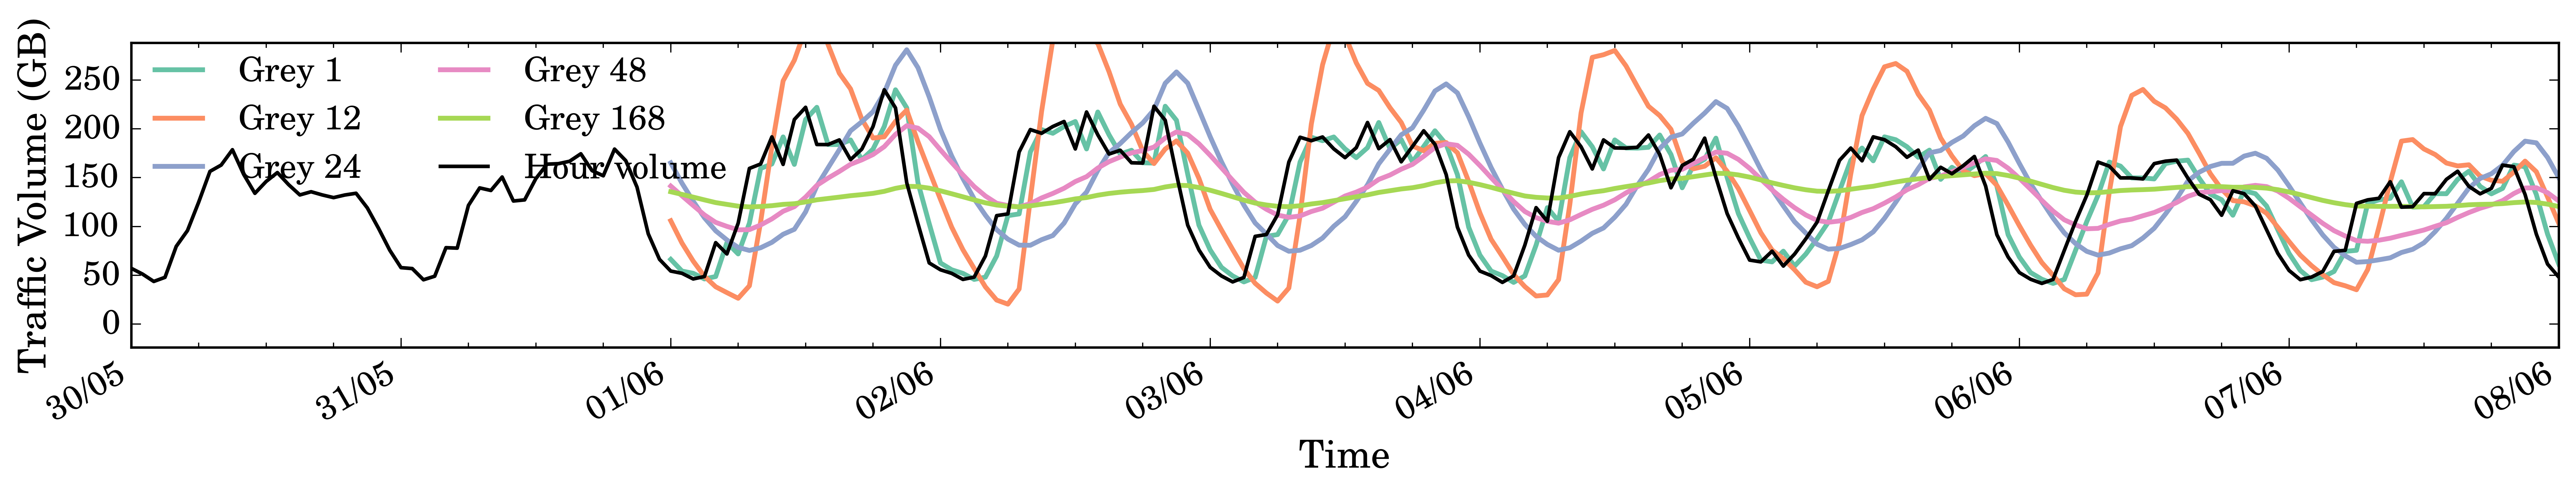
\includegraphics[width=\textwidth]{gfx/chap2/grey_sa.png}
                \caption{SA}
                \label{fig:grey_sa}
        \end{subfigure}
        \begin{subfigure}[b]{0.9\textwidth}
                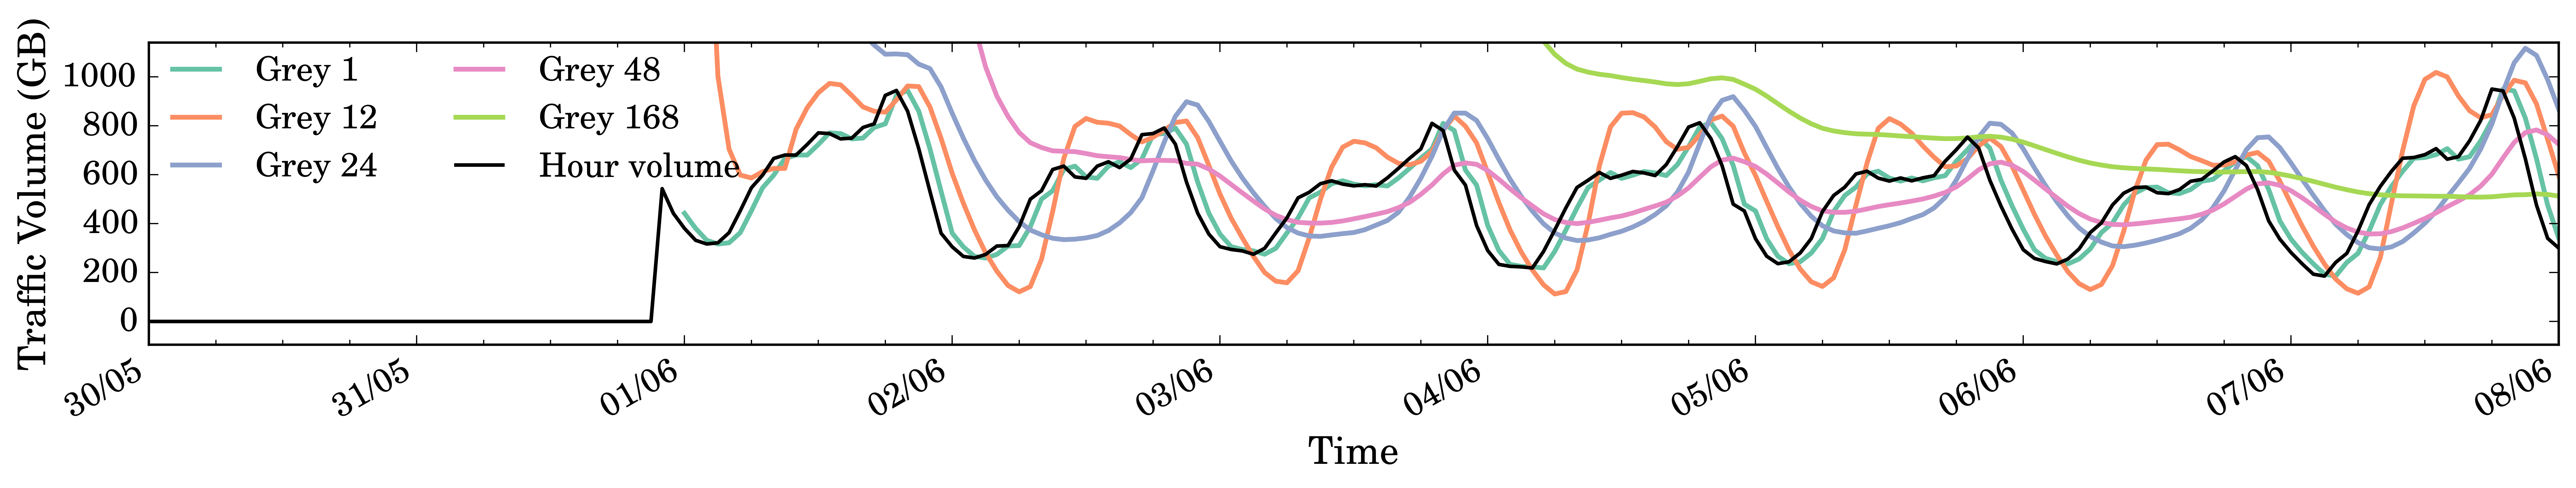
\includegraphics[width=\textwidth]{gfx/chap2/grey_sb.png}
                \caption{SB}
                \label{fig:grey_sb}
        \end{subfigure}
        \begin{subfigure}[b]{0.9\textwidth}
                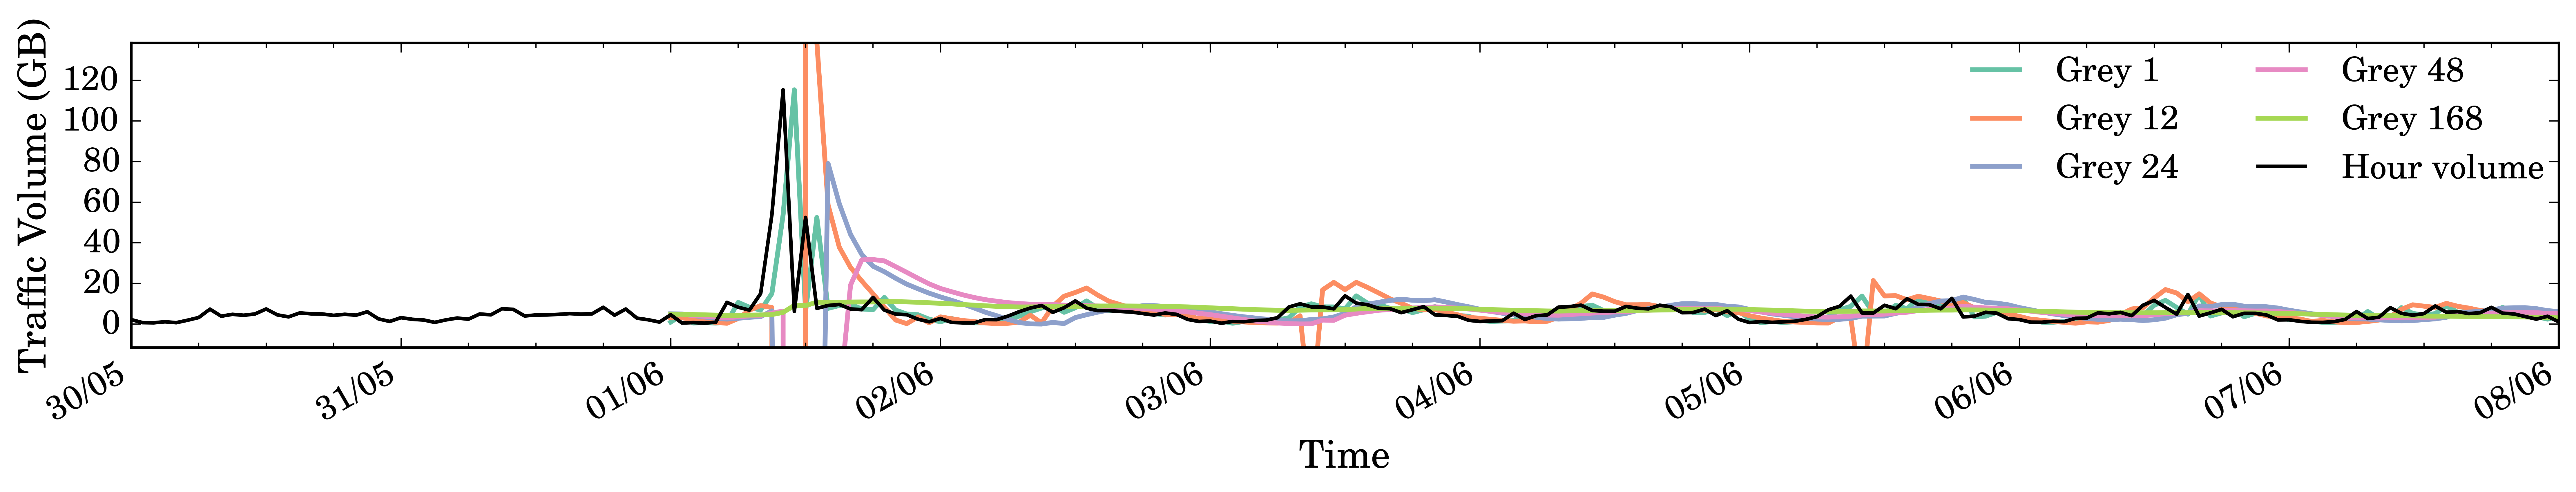
\includegraphics[width=\textwidth]{gfx/chap2/grey_sc.png}
                \caption{SC}
                \label{fig:grey_sc}
        \end{subfigure}
        \begin{subfigure}[b]{0.9\textwidth}
                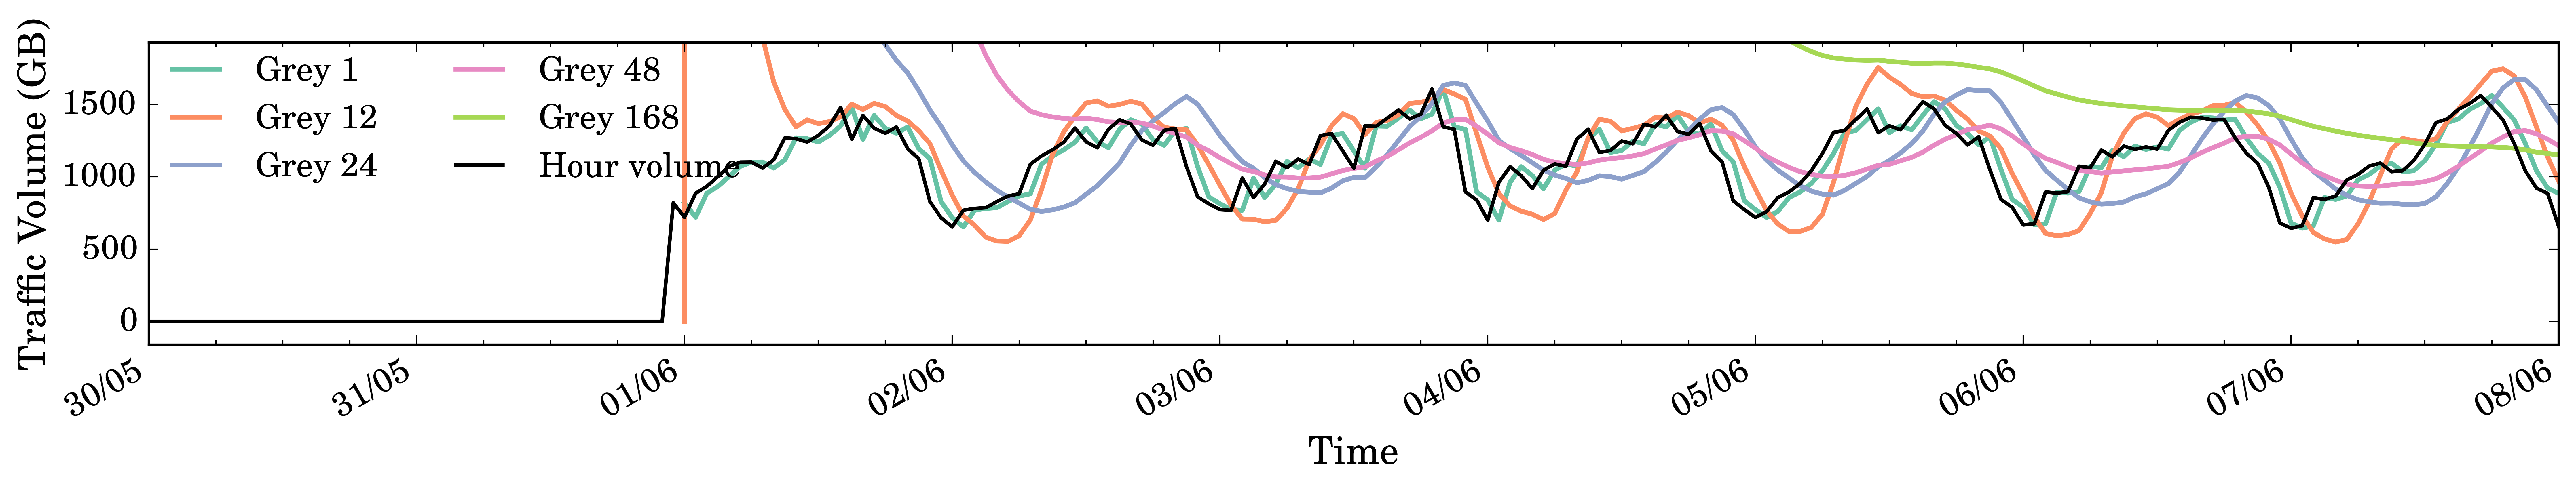
\includegraphics[width=\textwidth]{gfx/chap2/grey_sd.png}
                \caption{SD}
                \label{fig:grey_sd}
        \end{subfigure}
        \begin{subfigure}[b]{0.9\textwidth}
                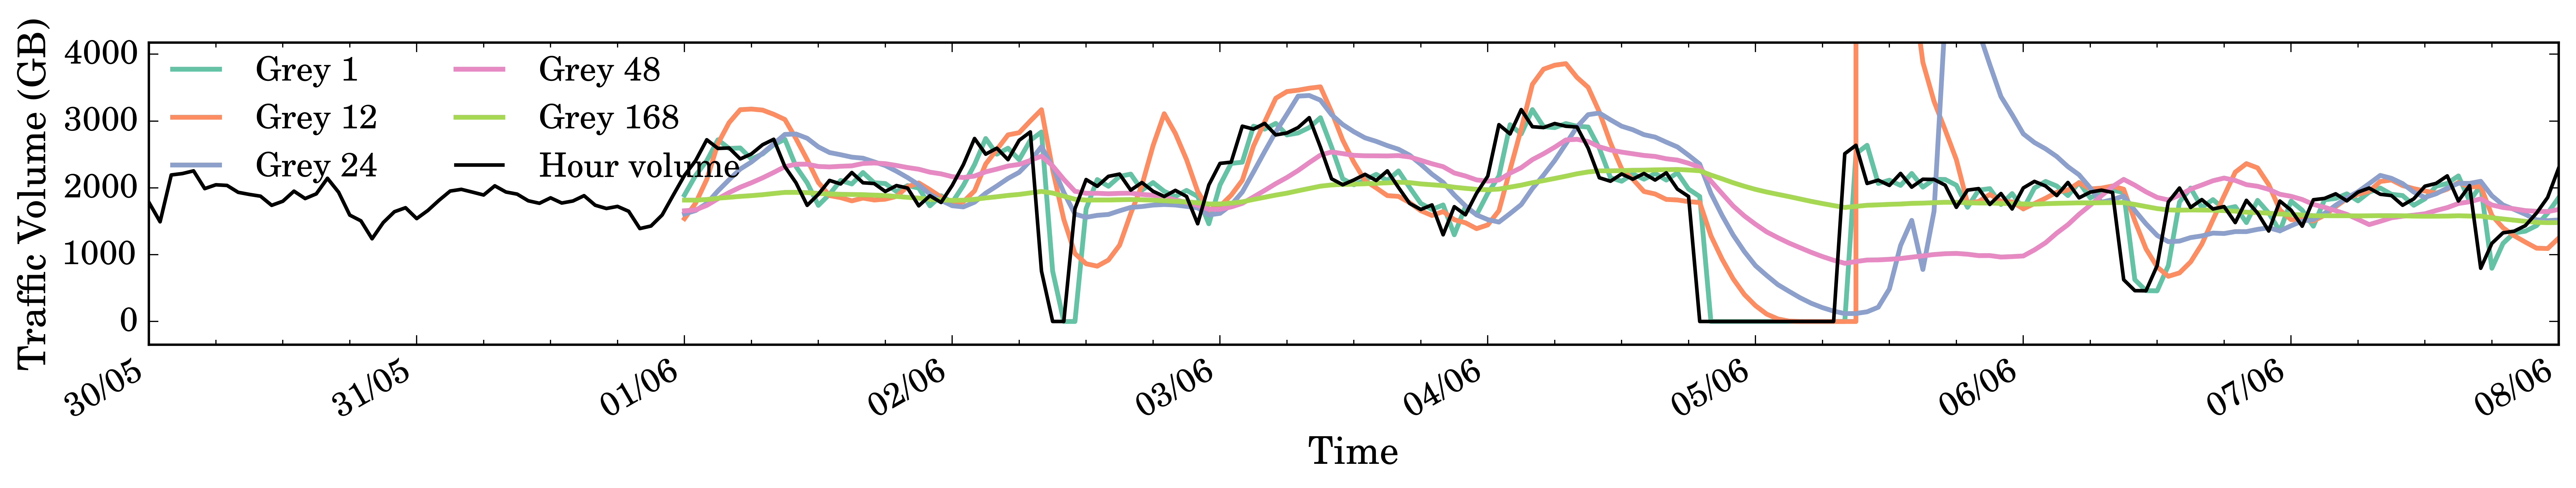
\includegraphics[width=\textwidth]{gfx/chap2/grey_se.png}
                \caption{SE}
                \label{fig:grey_se}
        \end{subfigure}
        \begin{subfigure}[b]{0.9\textwidth}
                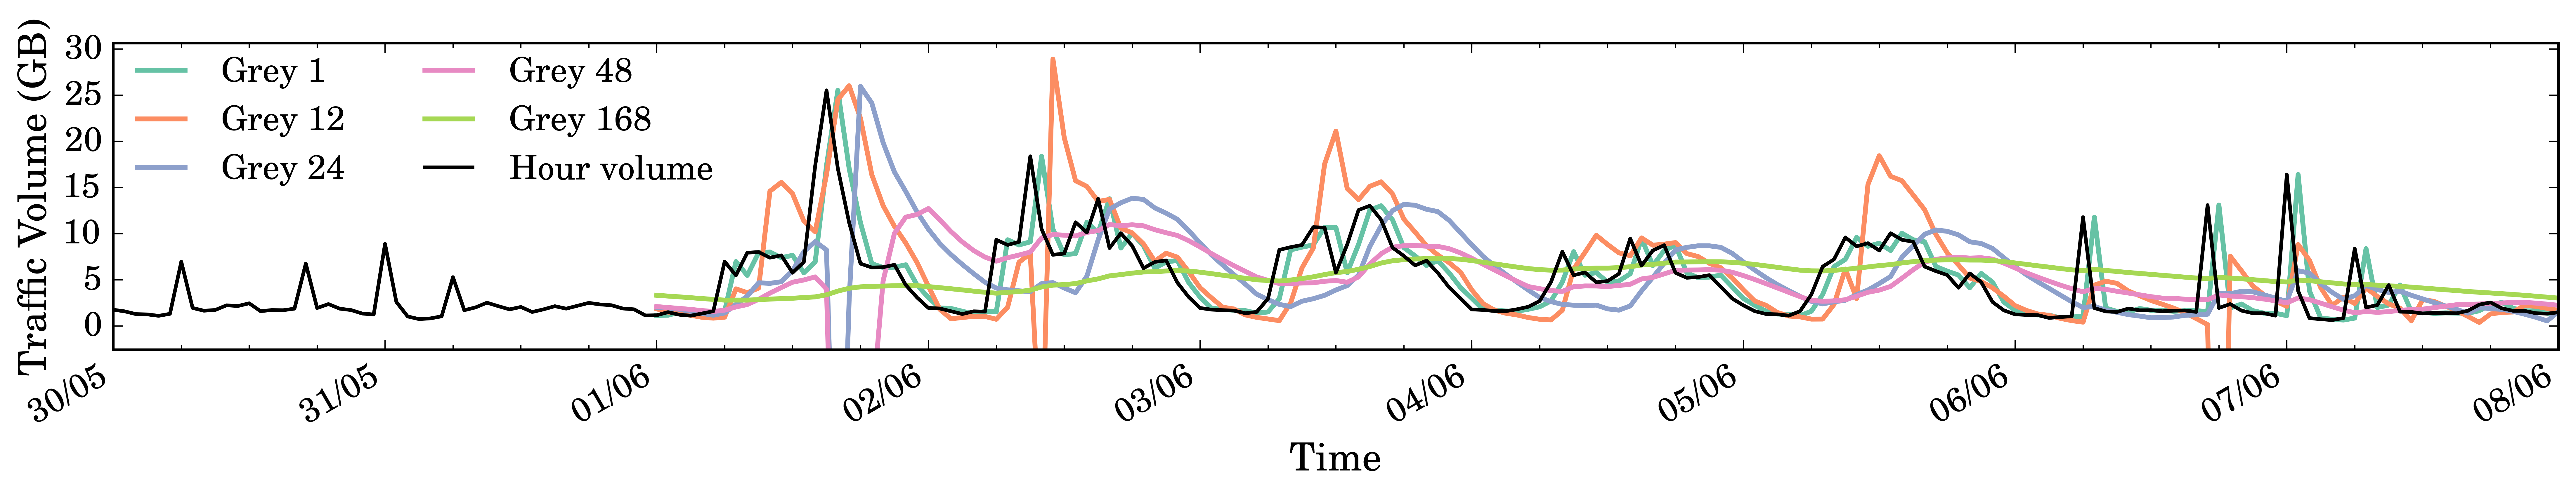
\includegraphics[width=\textwidth]{gfx/chap2/grey_sf.png}
                \caption{SF}
                \label{fig:grey_sf}
        \end{subfigure}
        \begin{subfigure}[b]{0.9\textwidth}
                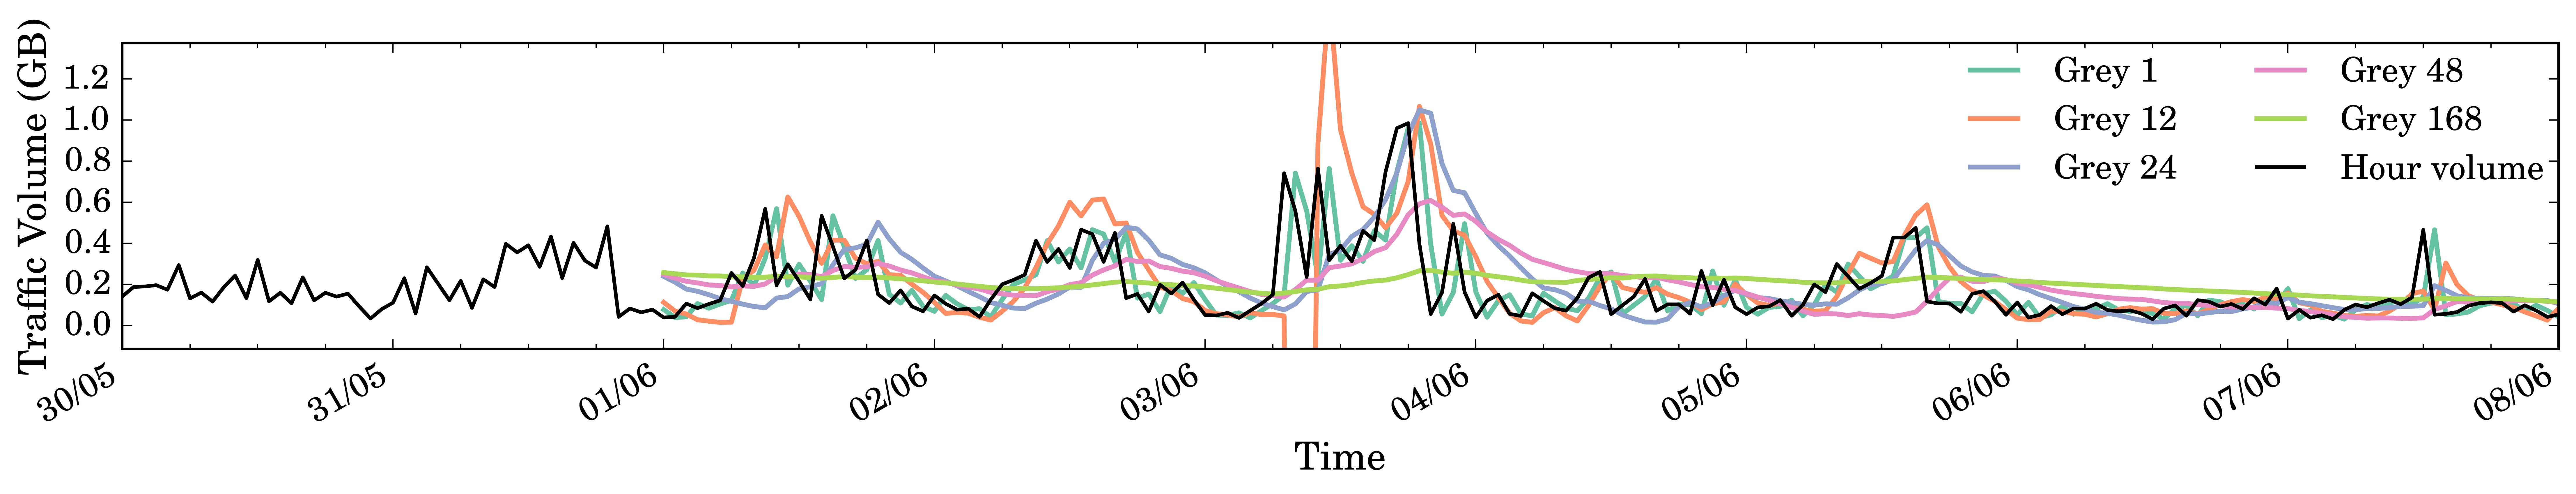
\includegraphics[width=\textwidth]{gfx/chap2/grey_sg.png}
                \caption{SG}
                \label{fig:grey_sg}
        \end{subfigure}
        \begin{subfigure}[b]{0.9\textwidth}
                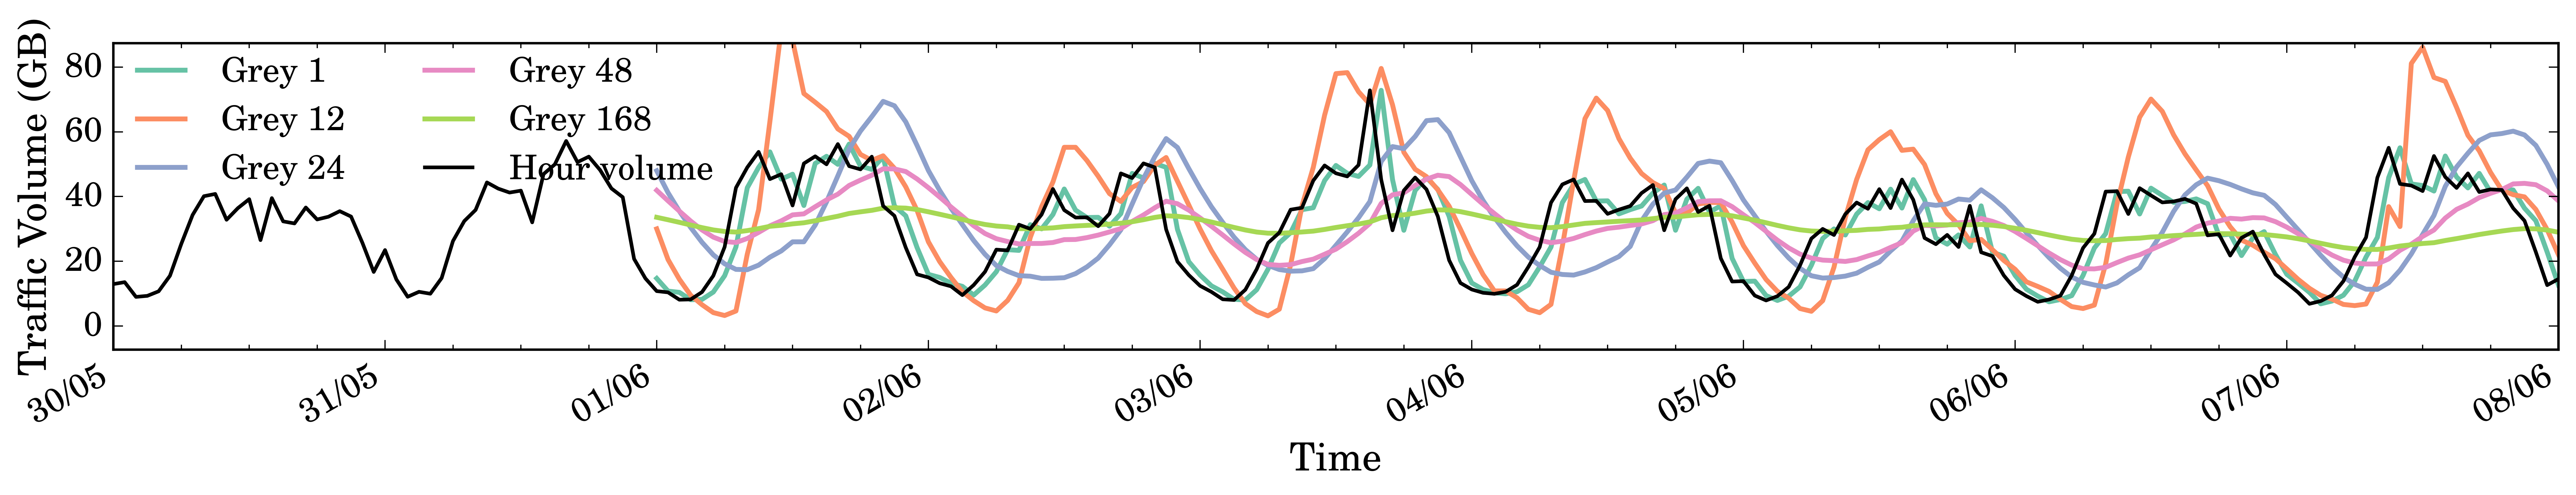
\includegraphics[width=\textwidth]{gfx/chap2/grey_sh.png}
                \caption{SH}
                \label{fig:grey_sh}
        \end{subfigure}
        \begin{subfigure}[b]{0.9\textwidth}
                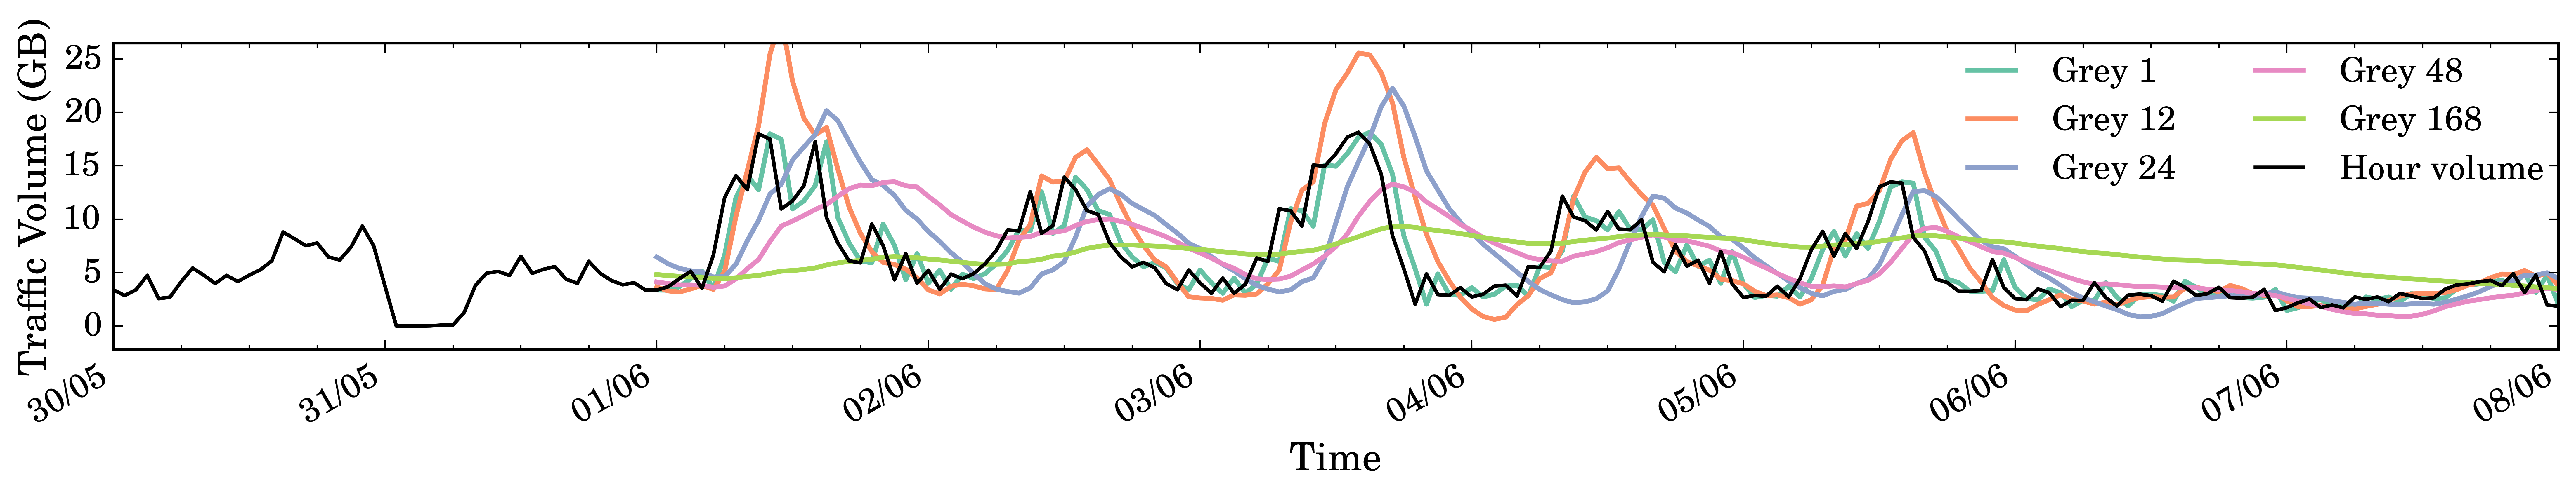
\includegraphics[width=\textwidth]{gfx/chap2/grey_si.png}
                \caption{SI}
                \label{fig:grey_si}
        \end{subfigure}
\caption{Predict total hour volume using $GM(1,1)$ with different historical record lengths for the week starting from June 1st, 2015.}
\label{fig:grey}
\end{figure}

%\marginpar{Why grey model performs poorly?}
On the other hand, the hour volume coverage by grey model drops as we increase the historical records length and is in general much worse than the metrics proposed in this work. 
In order to understand the underlying reason, we used $GM(1,1)$ model described above to dynamically predict the total hour volume of all prefixes, which is normally much more regular and smoother than the volume series of individual prefixes, Figure~\ref{fig:grey}.

%\marginpar{overreact to sudden value change.}
For site SB and SD, we miss the hour volume data for the week starting from May 25th. 
$GM(1,1)$ model using records of last $168$ suffer a lot from  data missing and converge extremely slow to actual traffic volume. 
However, such sudden change in value is not unexpected, since bursty prefixes can bring huge amount of traffic within in a short duration and then remain silent over days. Such prefixes are commonly seen on SC, SF, SG judging from their burstiness index in Table~\ref{tab:bi}.
This explains why grey model leads to fairly low volume coverage in Figure~\ref{fig:cvg_sc}. 

%\marginpar{delayed response to value change}
Furthermore, in Figure~\ref{fig:grey_sb}, Figure~\ref{fig:grey_sc} and as well in others, we can see that grey model reacts to volume variations in an obviously delayed manner. 
Longer the historical records length is, longer grey model delays the variations of actual trace.  
This behavior could be fatal in the presence of bursty prefixes.
We can observe considerably large pikes in both directions several hours after the volume burst in Figure~\ref{fig:grey_sc}, which might greatly disturb the prefix selection during those periods and consequently cause low volume coverage.

Compared to grey model, metrics proposed in our work do not directly predict hour volumes of each prefix but rather are indirect measures of its importance in terms of volume. And analysis in Section~\ref{sec:dyna} showed that the overall coverage using these metrics are guaranteed by the traffic character itself.

\begin{figure}
\centering
		\centering
        \begin{subfigure}[b]{0.48\textwidth}
                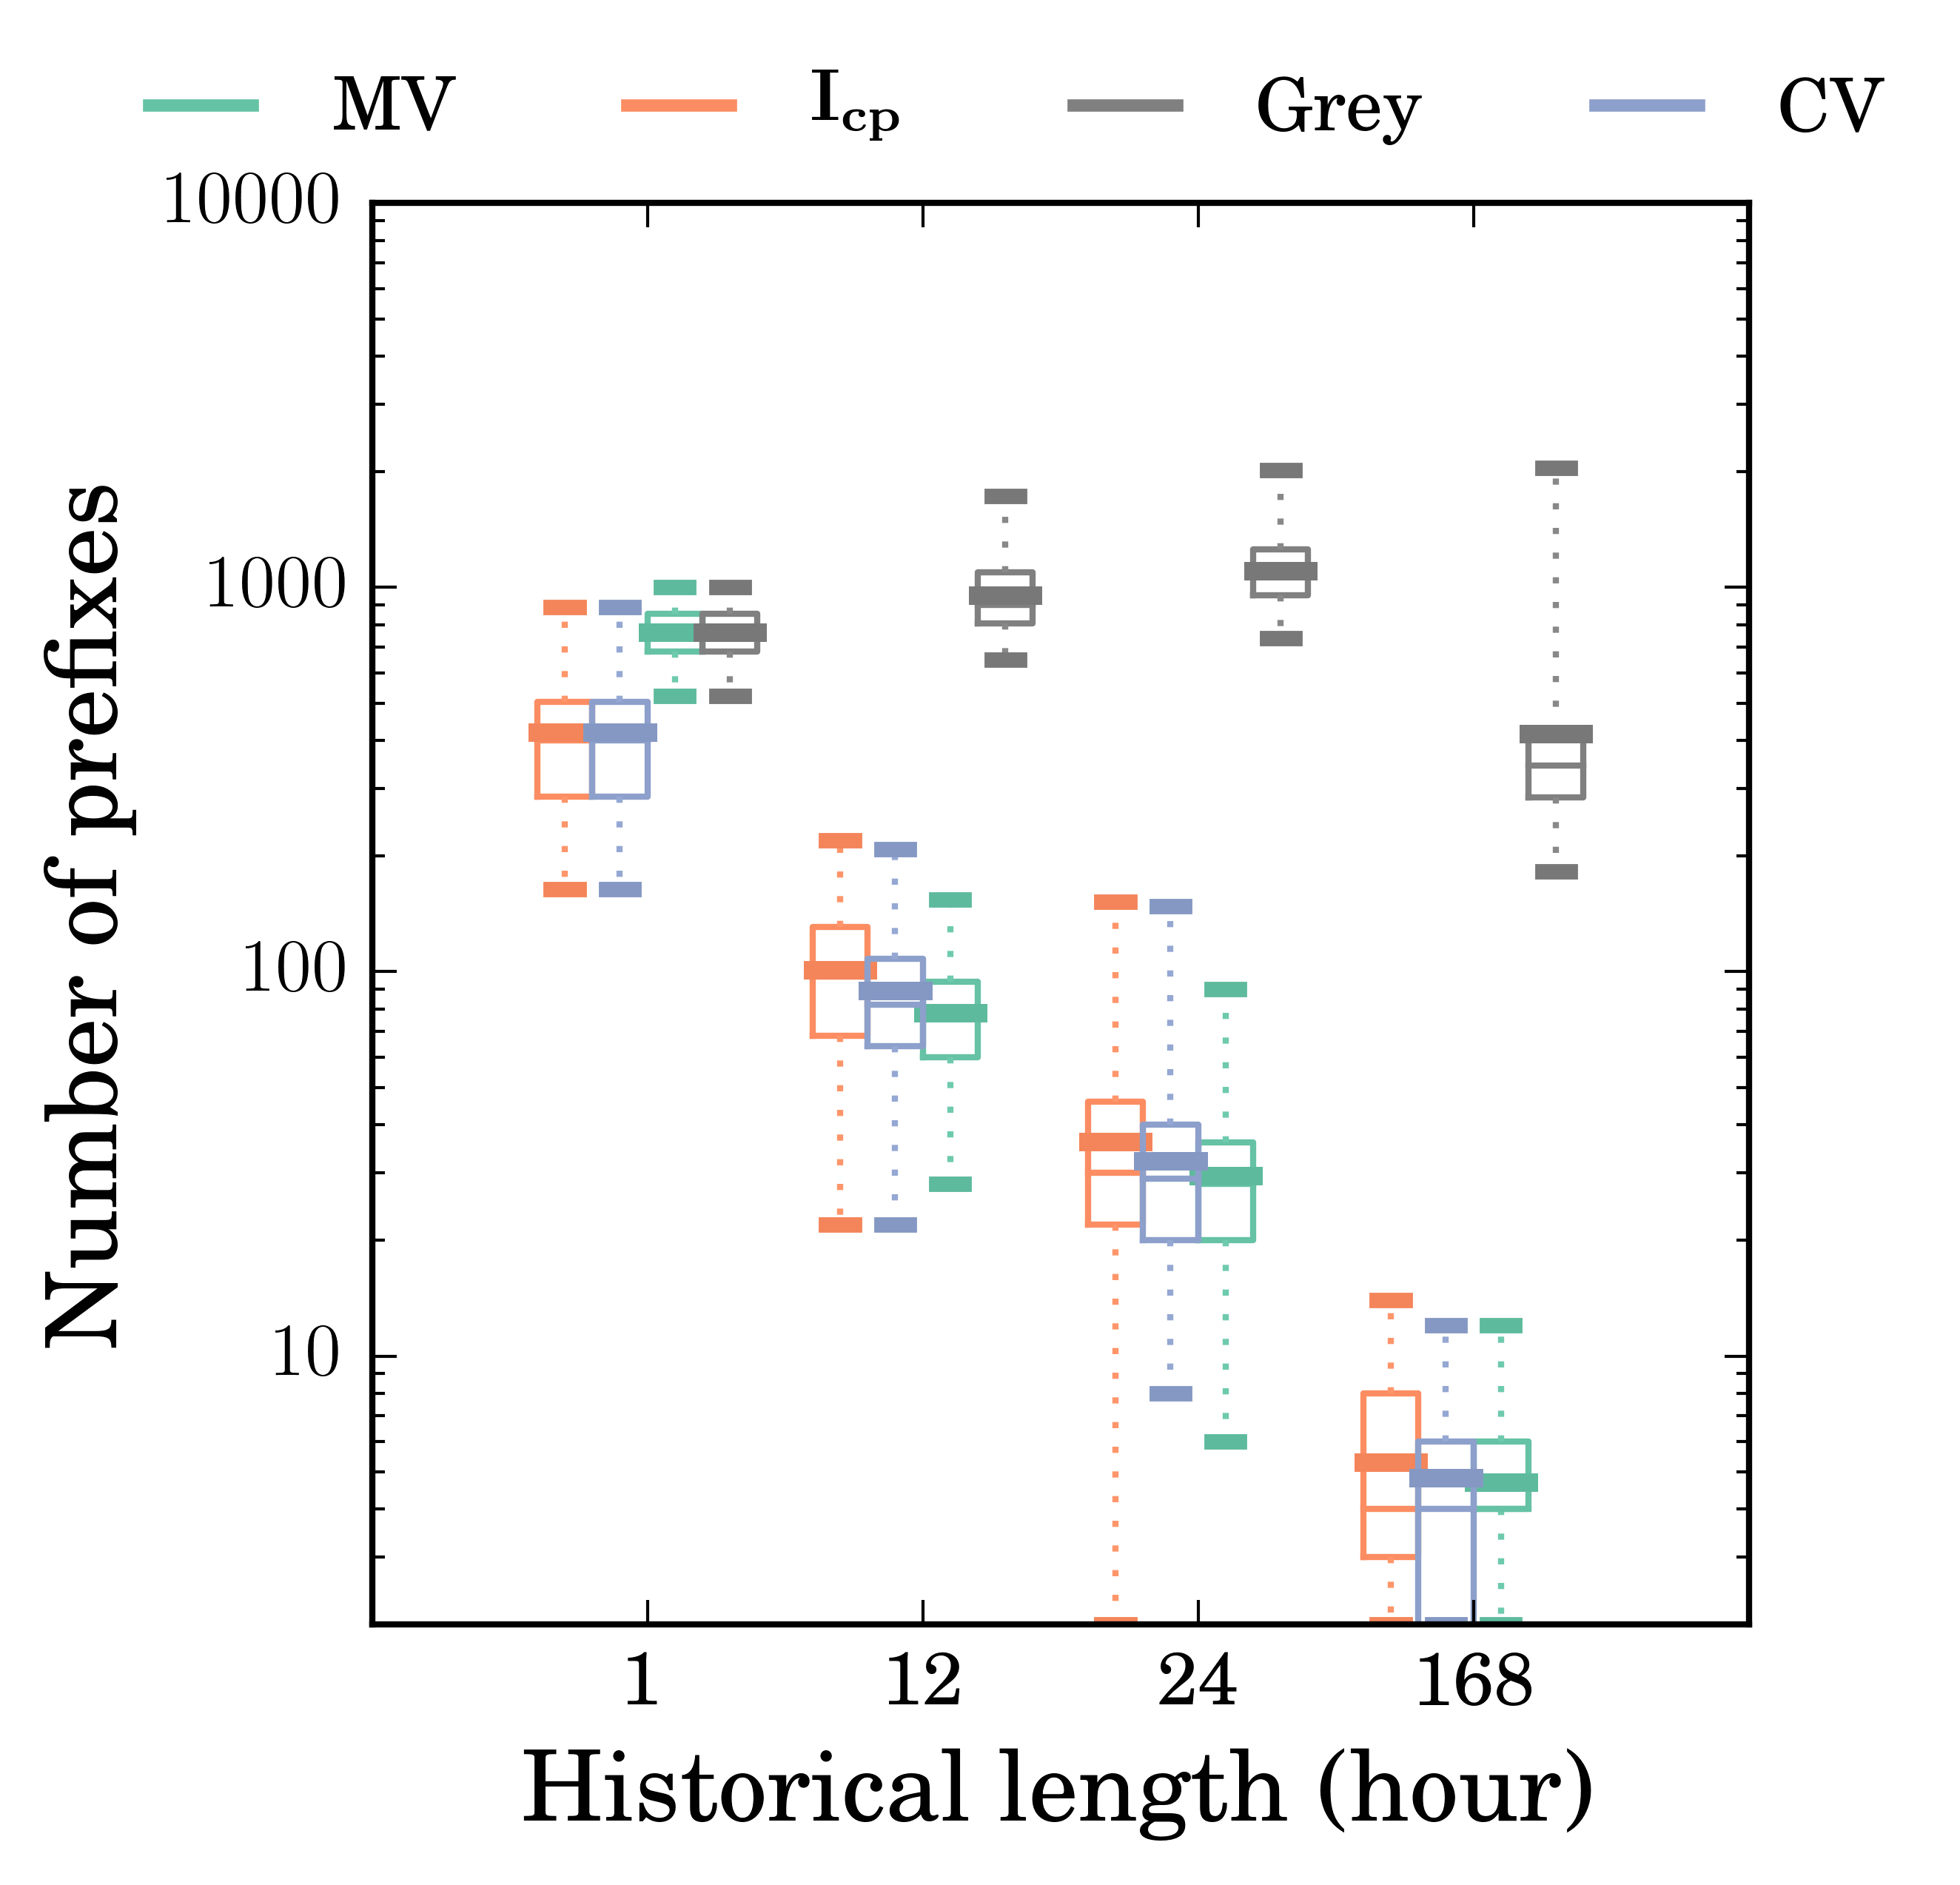
\includegraphics[width=\textwidth]{gfx/chap2/grey_churn_box_method_compare_fs_sa.png}
                \caption{SA}
                \label{fig:churn_sa}
        \end{subfigure}
        \begin{subfigure}[b]{0.48\textwidth}
                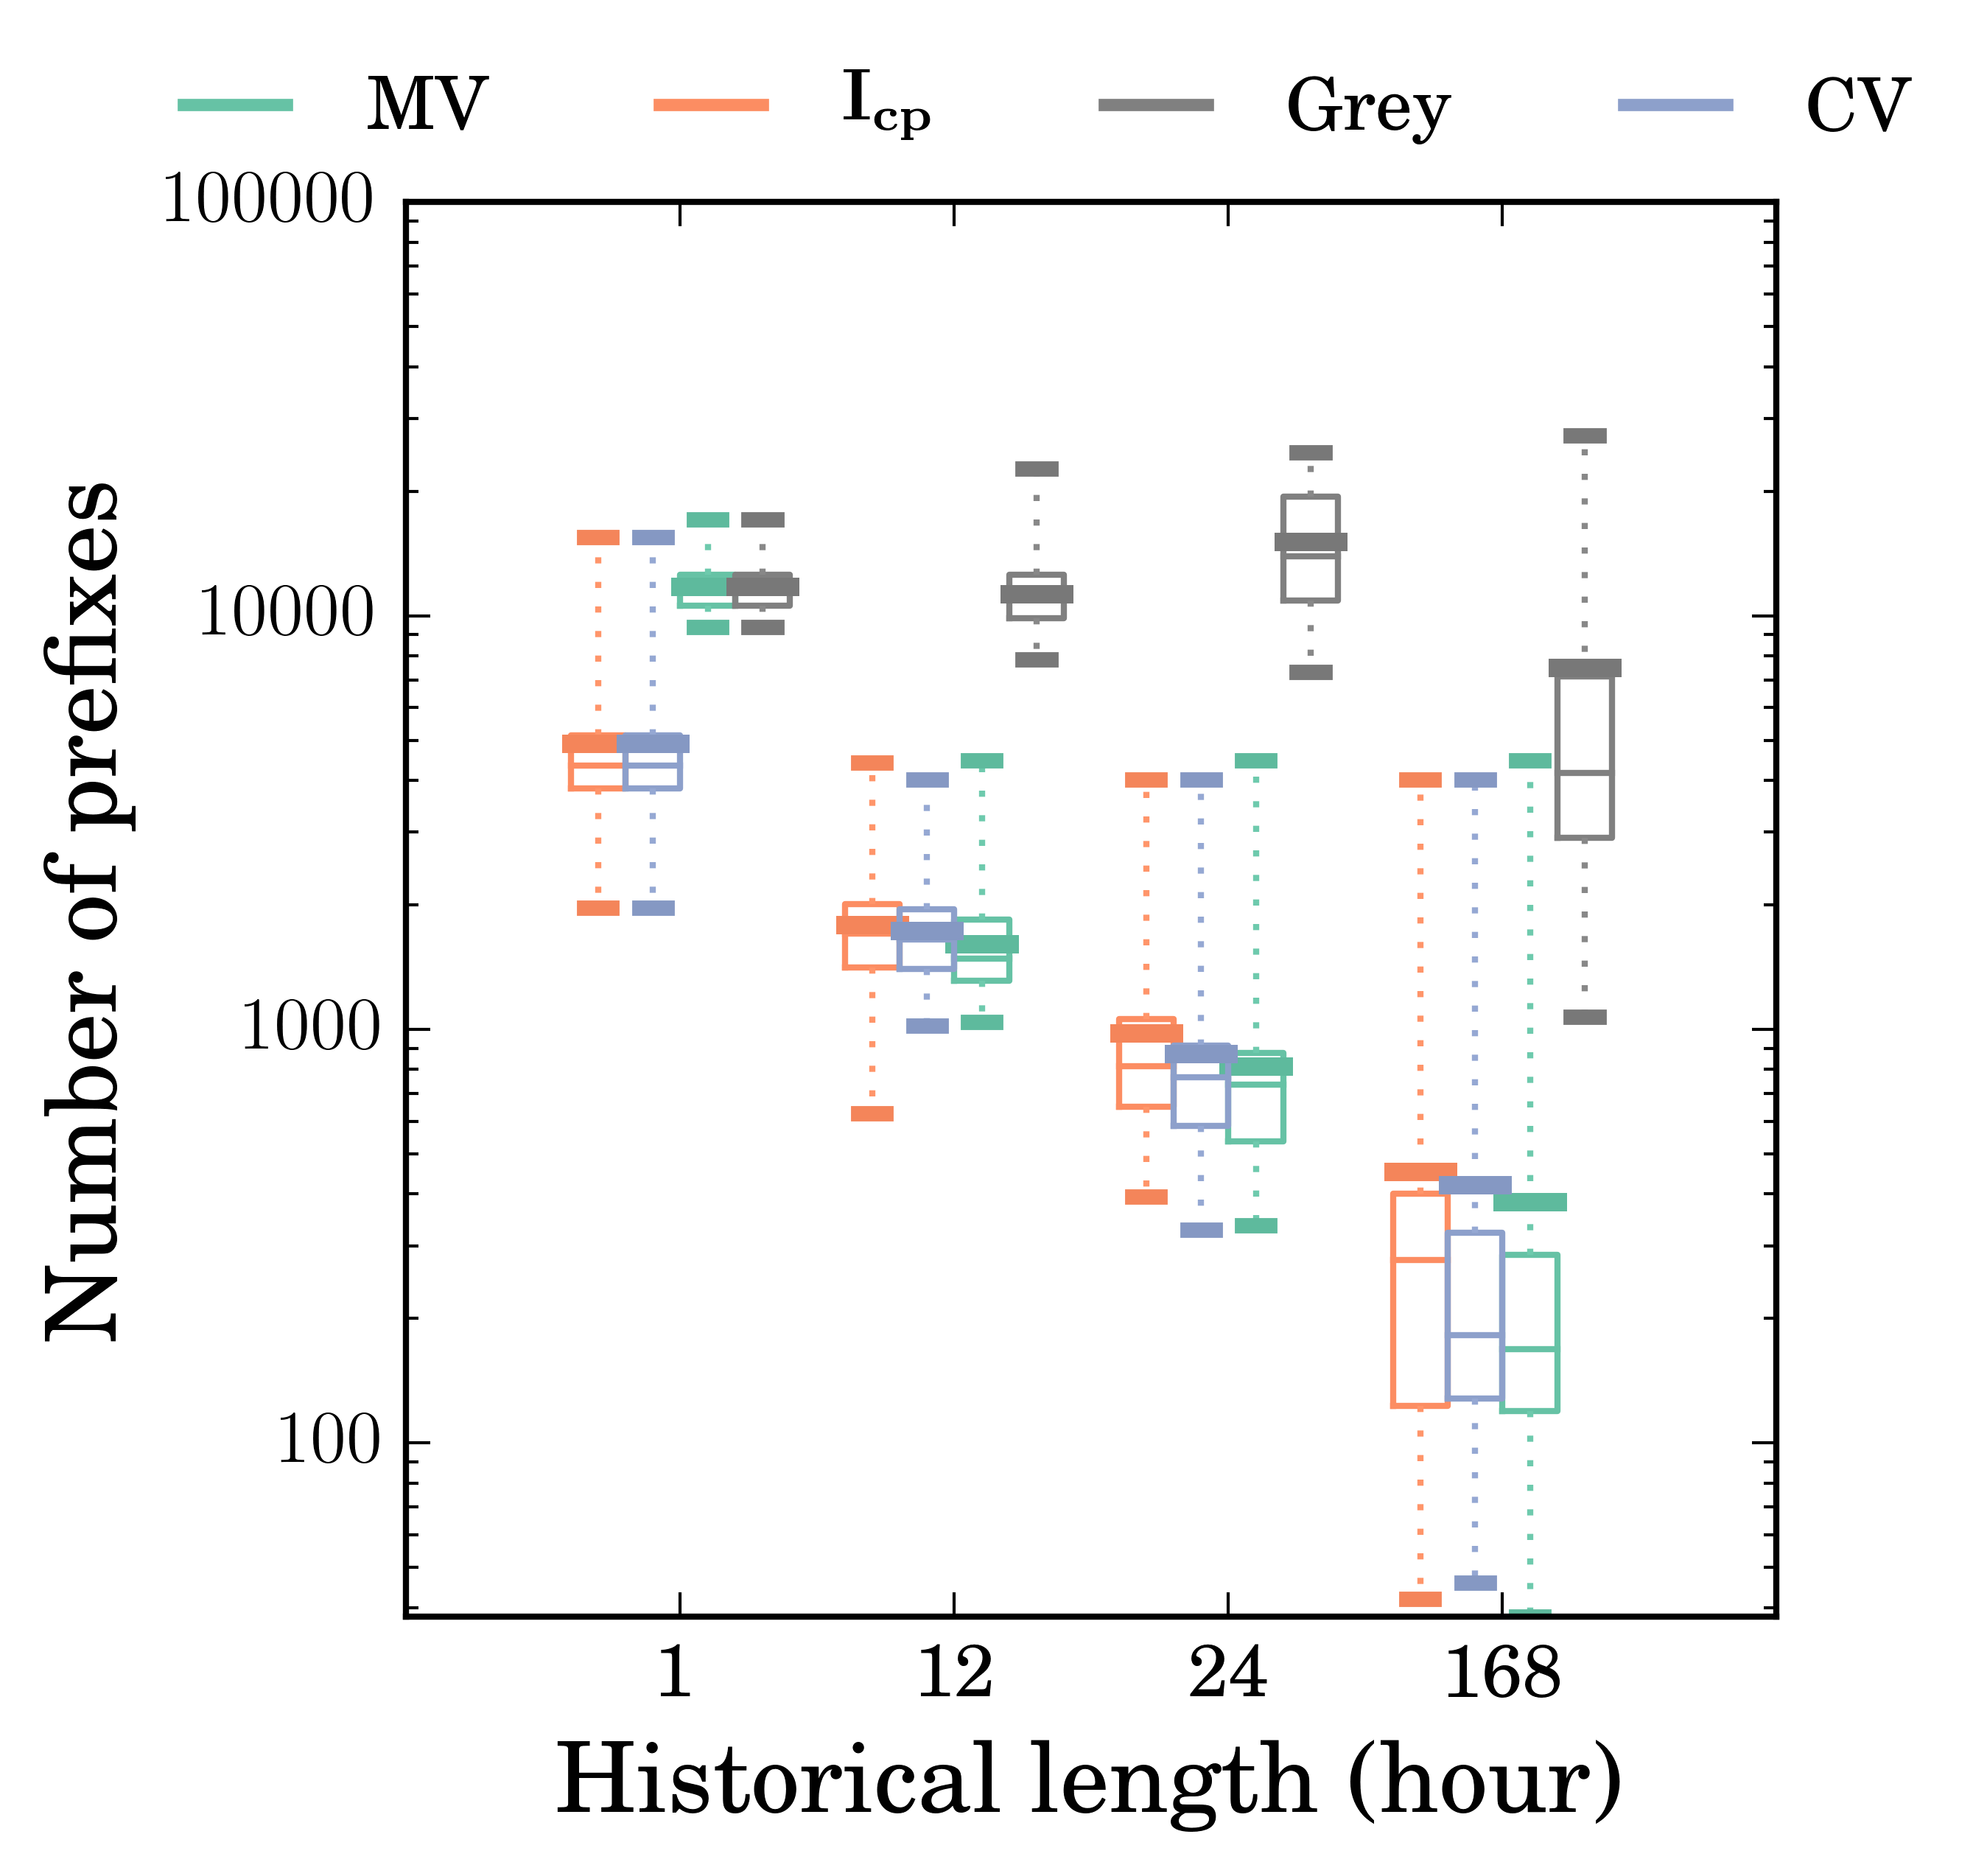
\includegraphics[width=\textwidth]{gfx/chap2/grey_churn_box_method_compare_fs_sb.png}
                \caption{SB}
                \label{fig:churn_sb}
        \end{subfigure}
        \begin{subfigure}[b]{0.48\textwidth}
                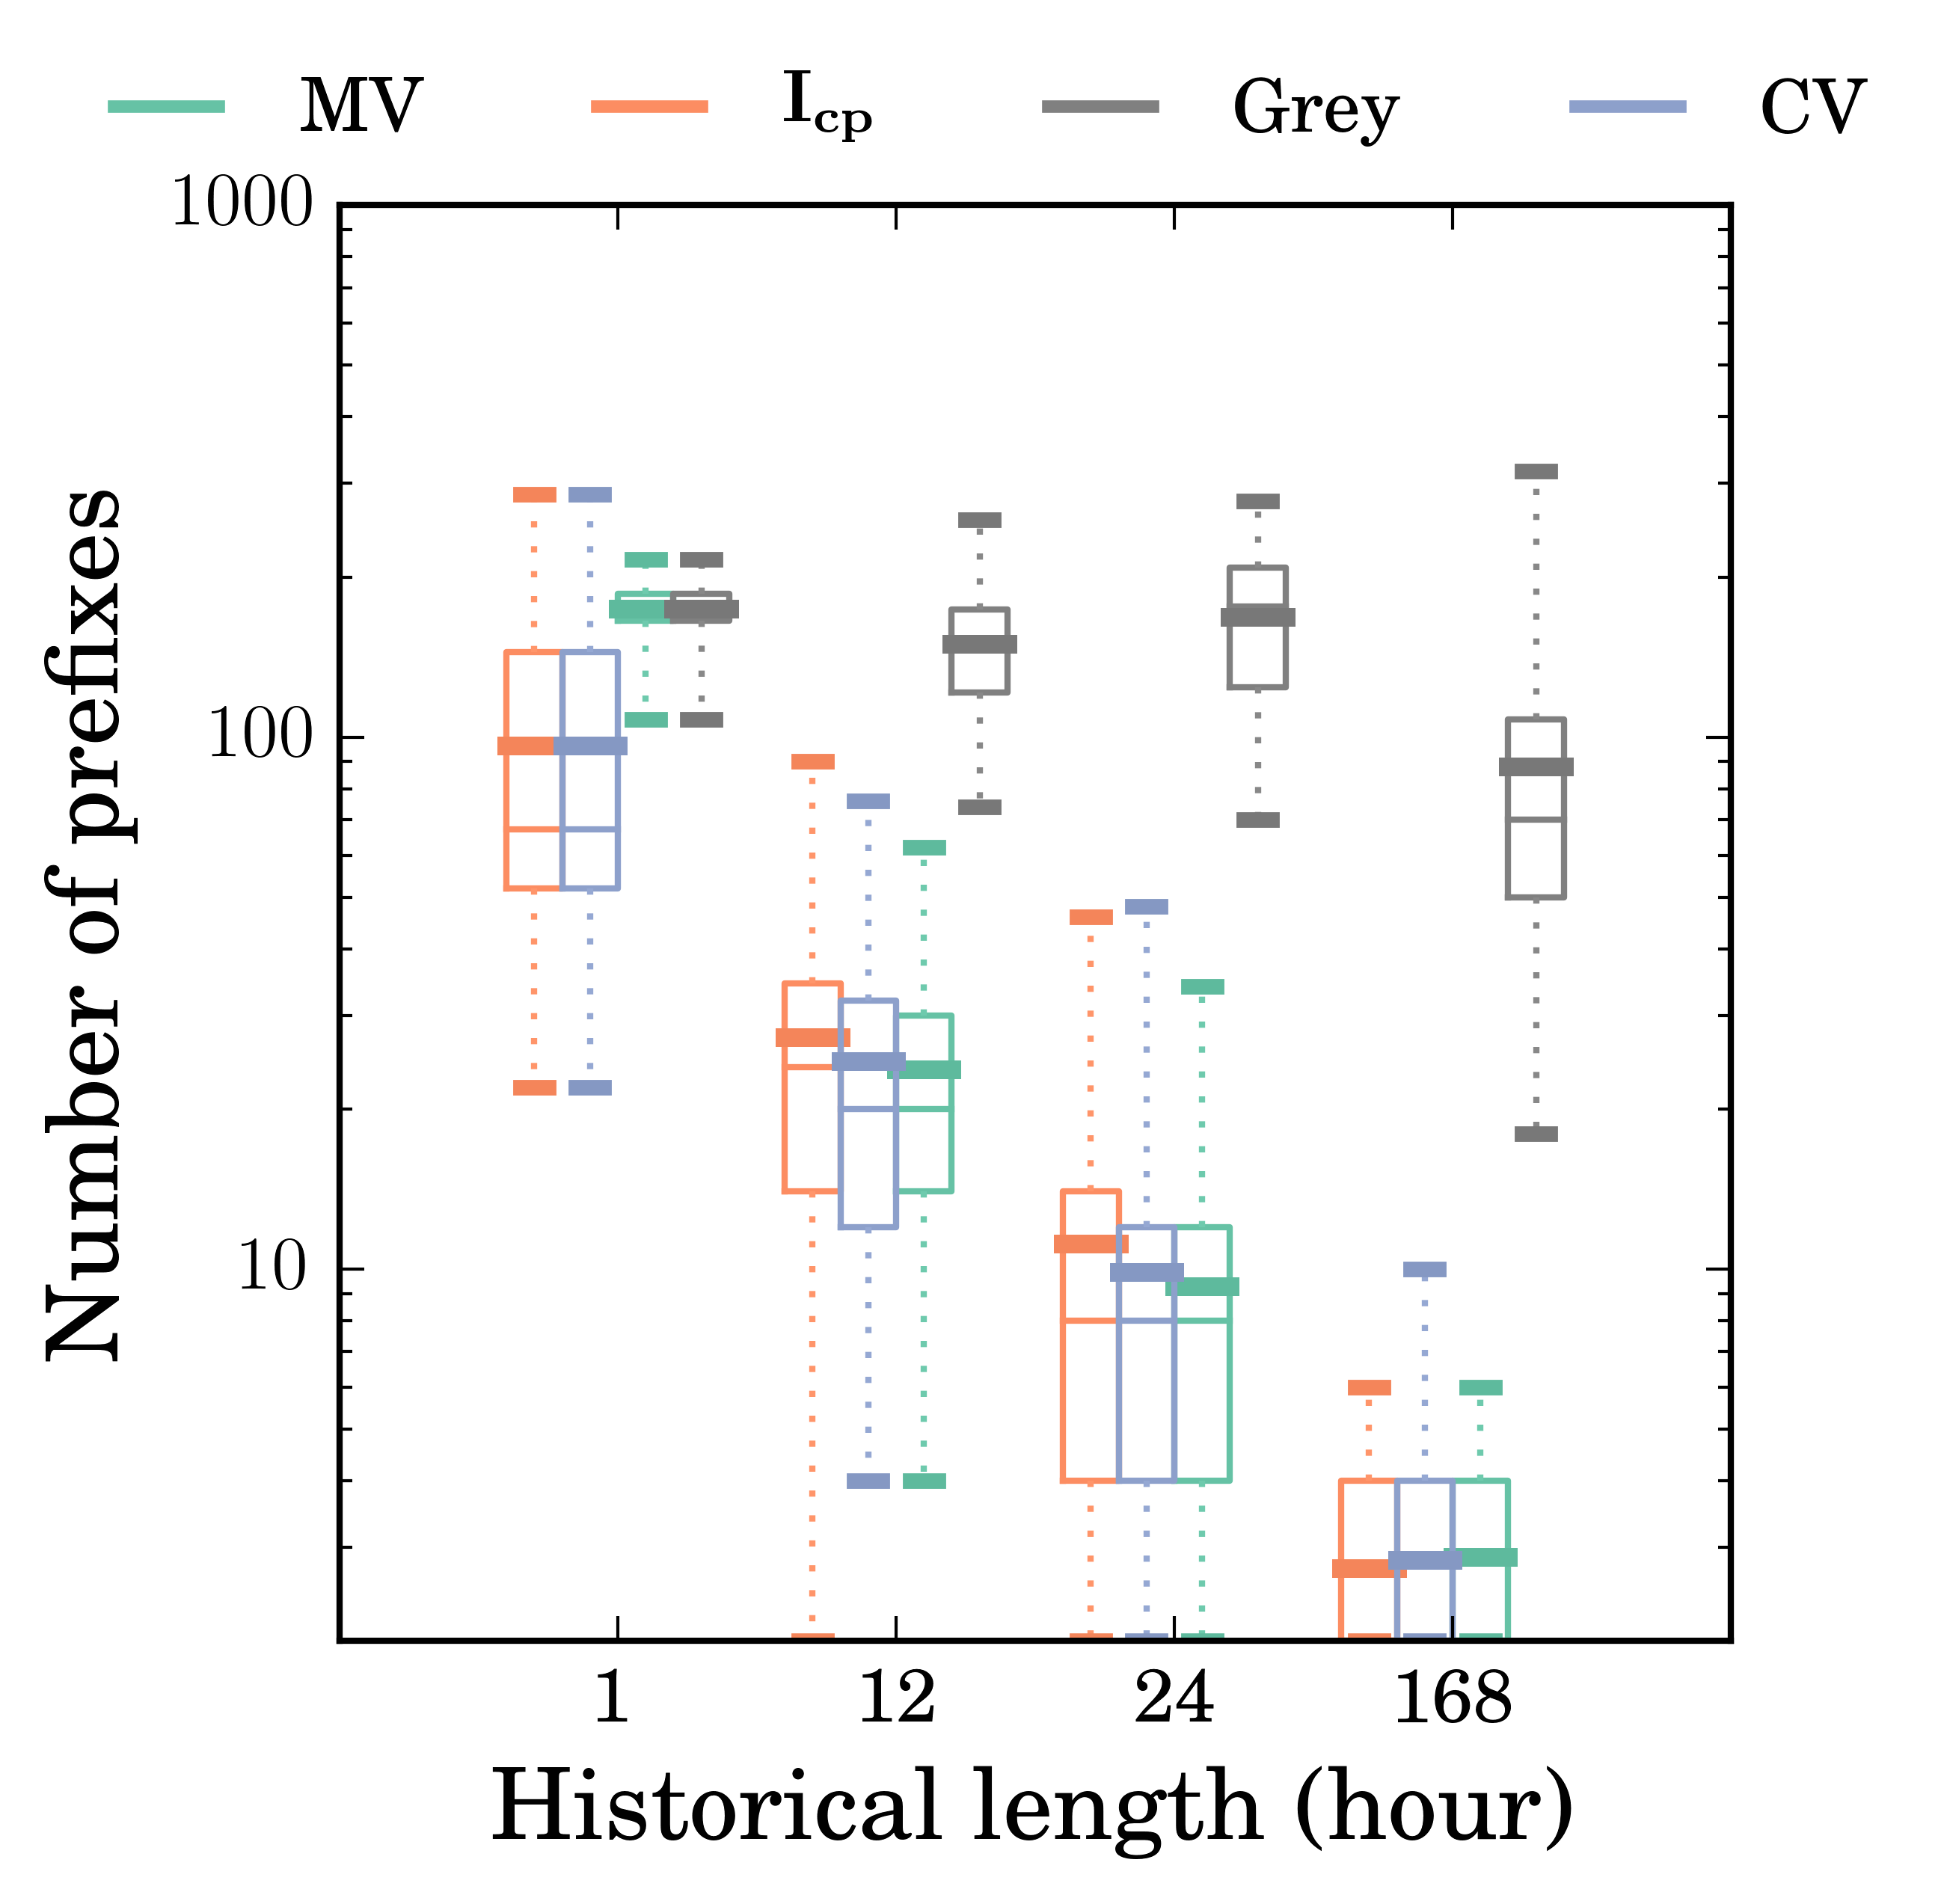
\includegraphics[width=\textwidth]{gfx/chap2/grey_churn_box_method_compare_fs_sc.png}
                \caption{SC}
                \label{fig:churn_sc}
        \end{subfigure}
        \begin{subfigure}[b]{0.48\textwidth}
                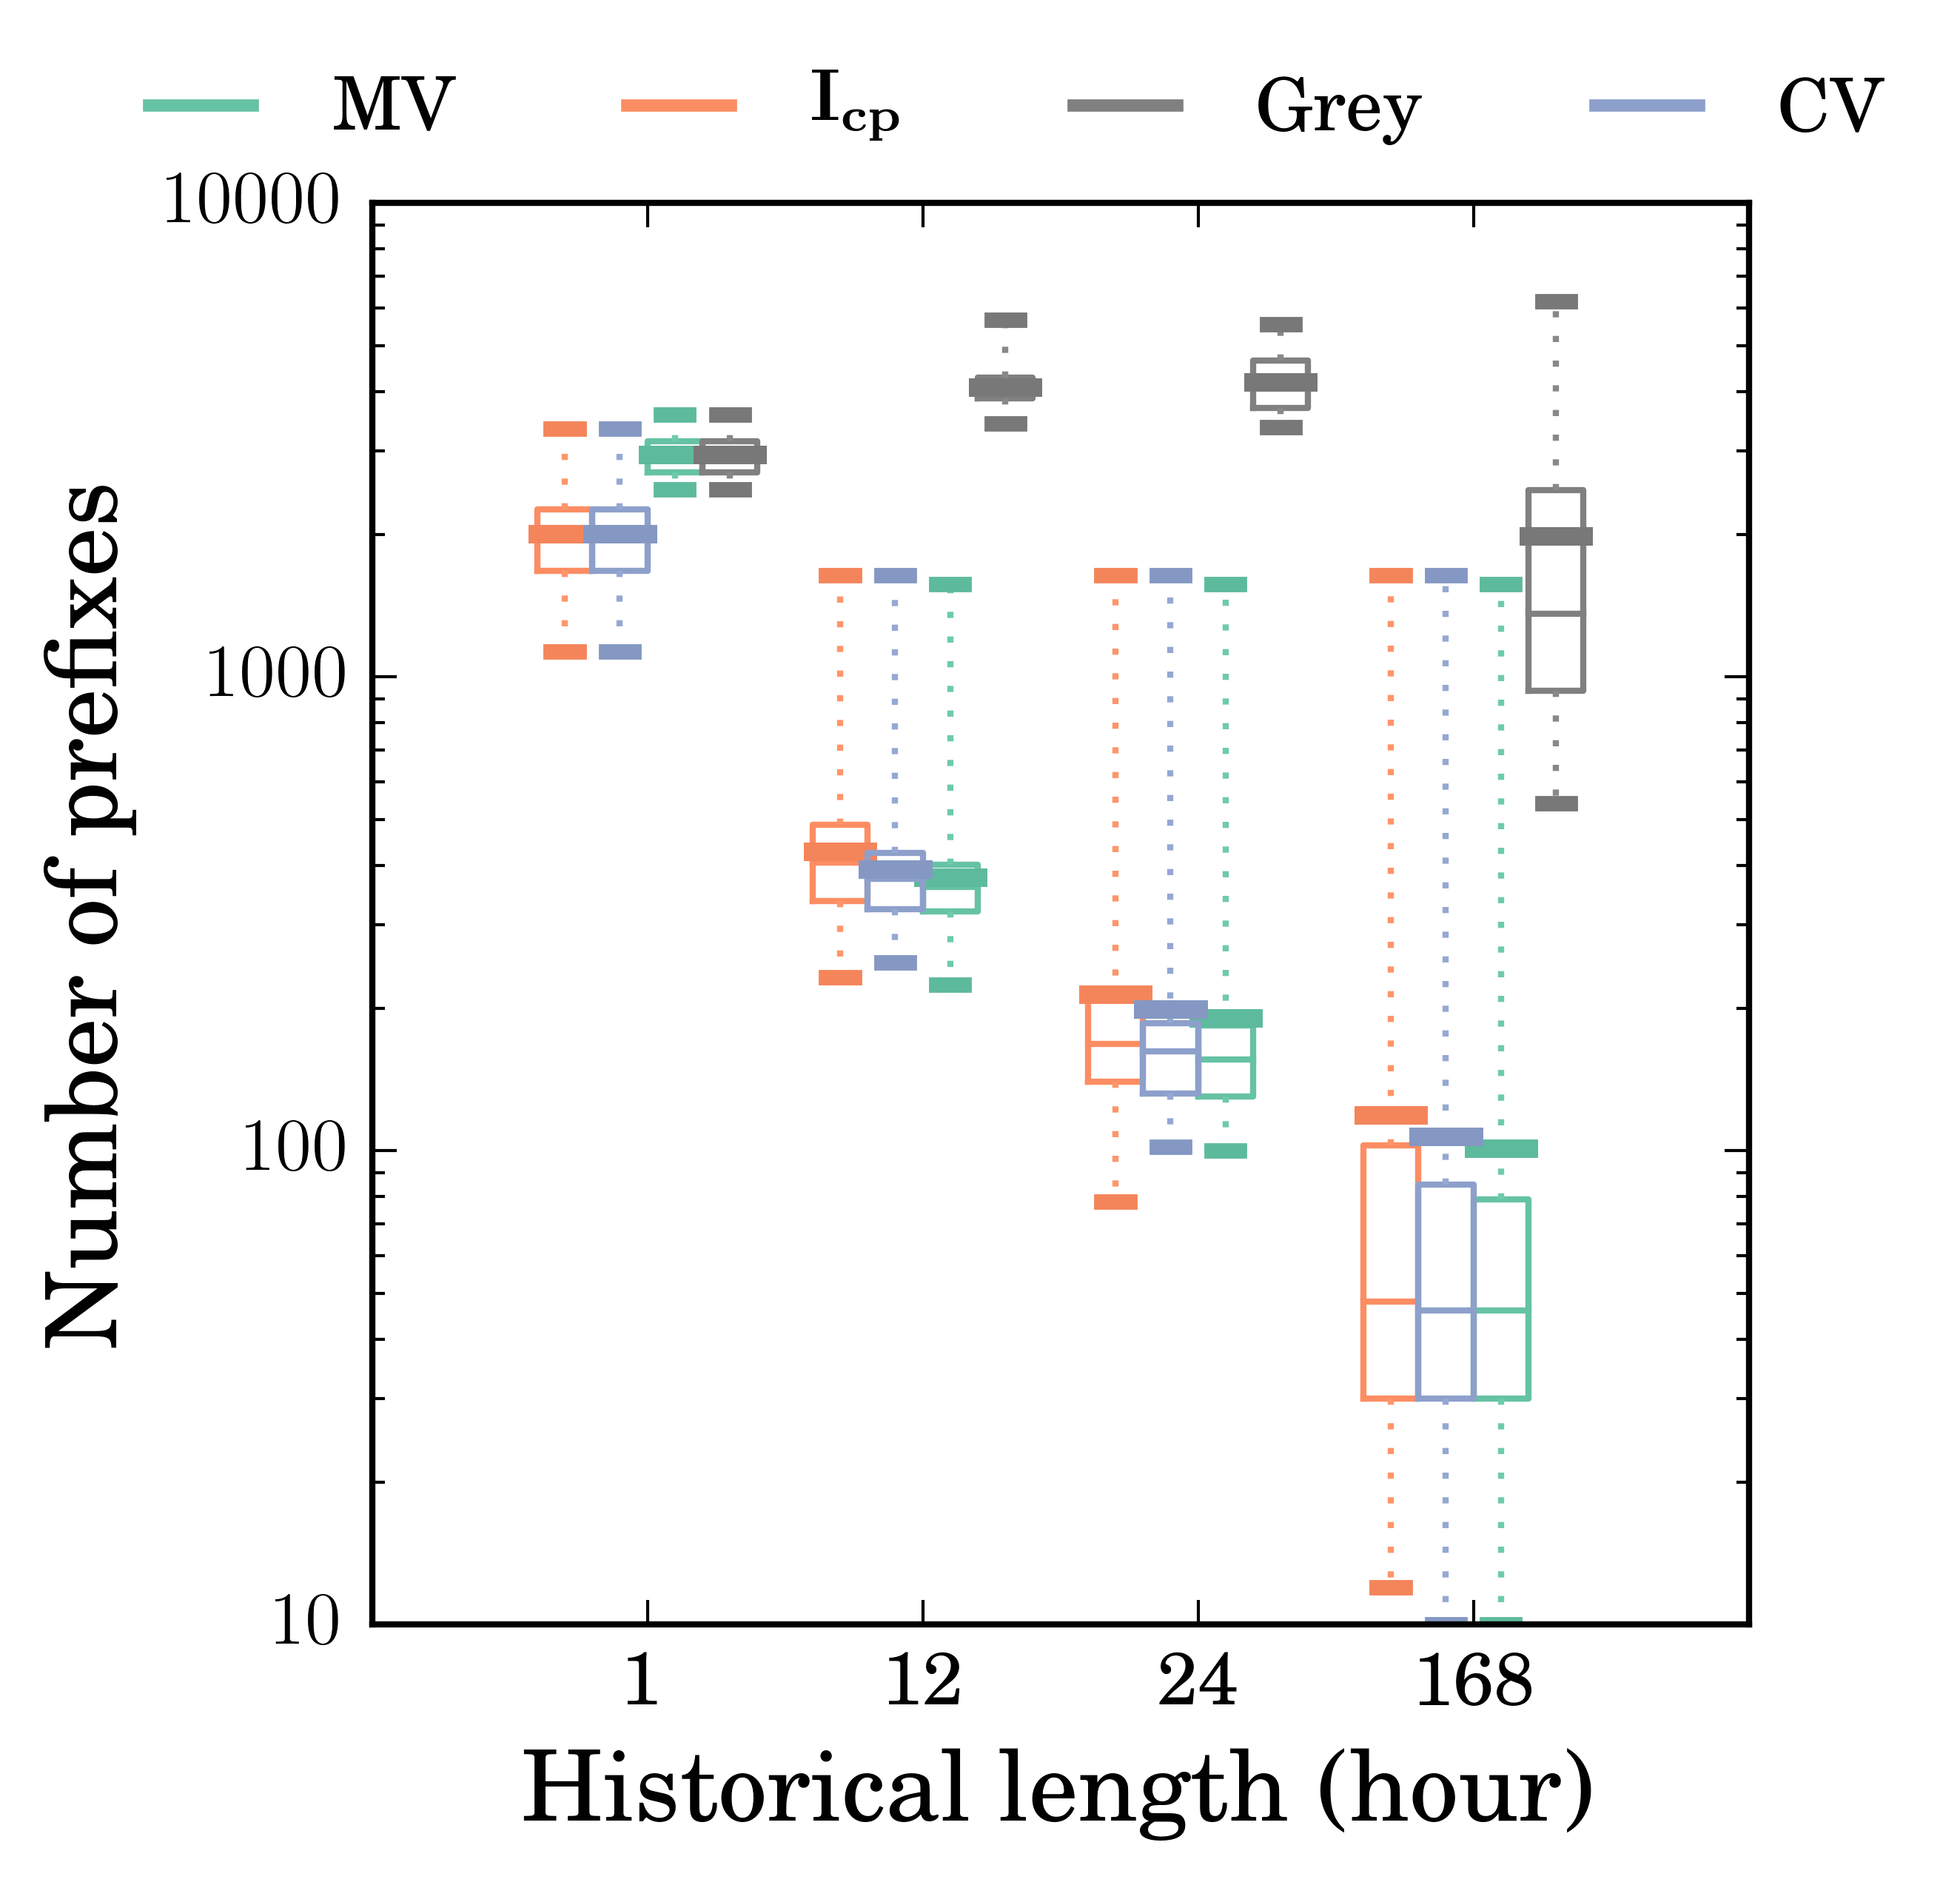
\includegraphics[width=\textwidth]{gfx/chap2/grey_churn_box_method_compare_fs_sd.png}
                \caption{SD}
                \label{fig:churn_sd}
        \end{subfigure}
        \begin{subfigure}[b]{0.48\textwidth}
                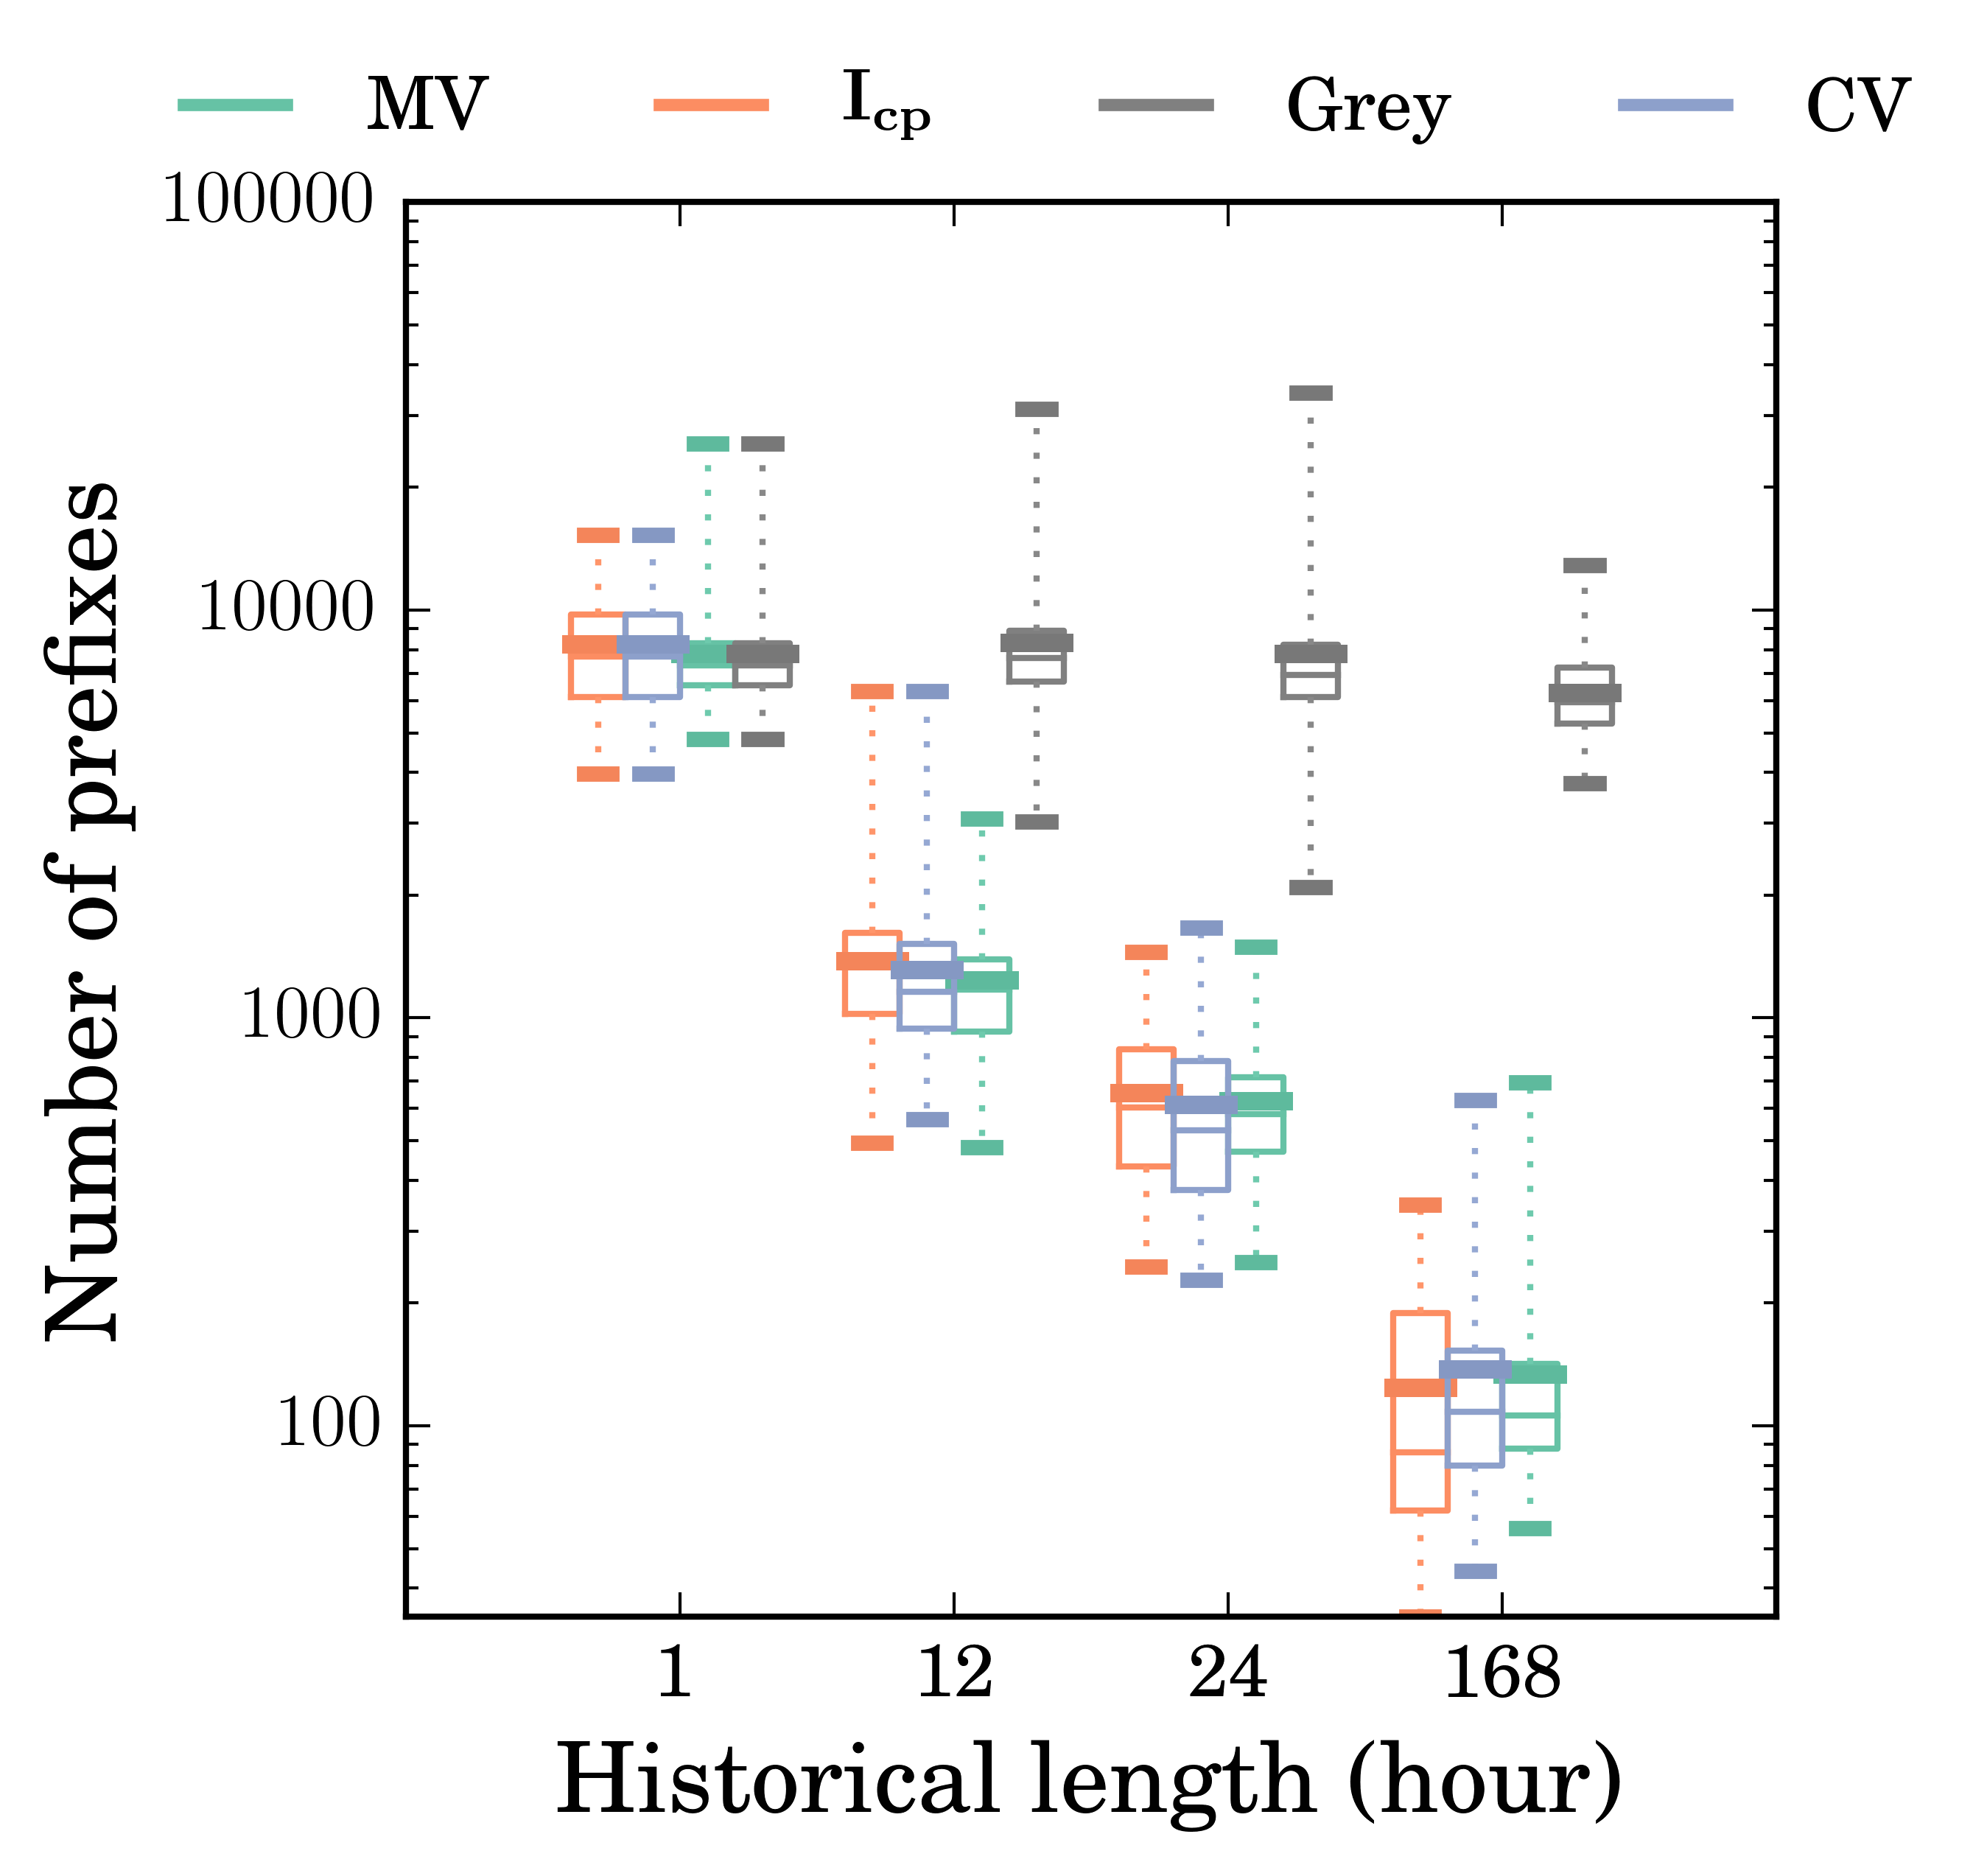
\includegraphics[width=\textwidth]{gfx/chap2/grey_churn_box_method_compare_fs_se.png}
                \caption{SE}
                \label{fig:churn_se}
        \end{subfigure}
        \begin{subfigure}[b]{0.48\textwidth}
                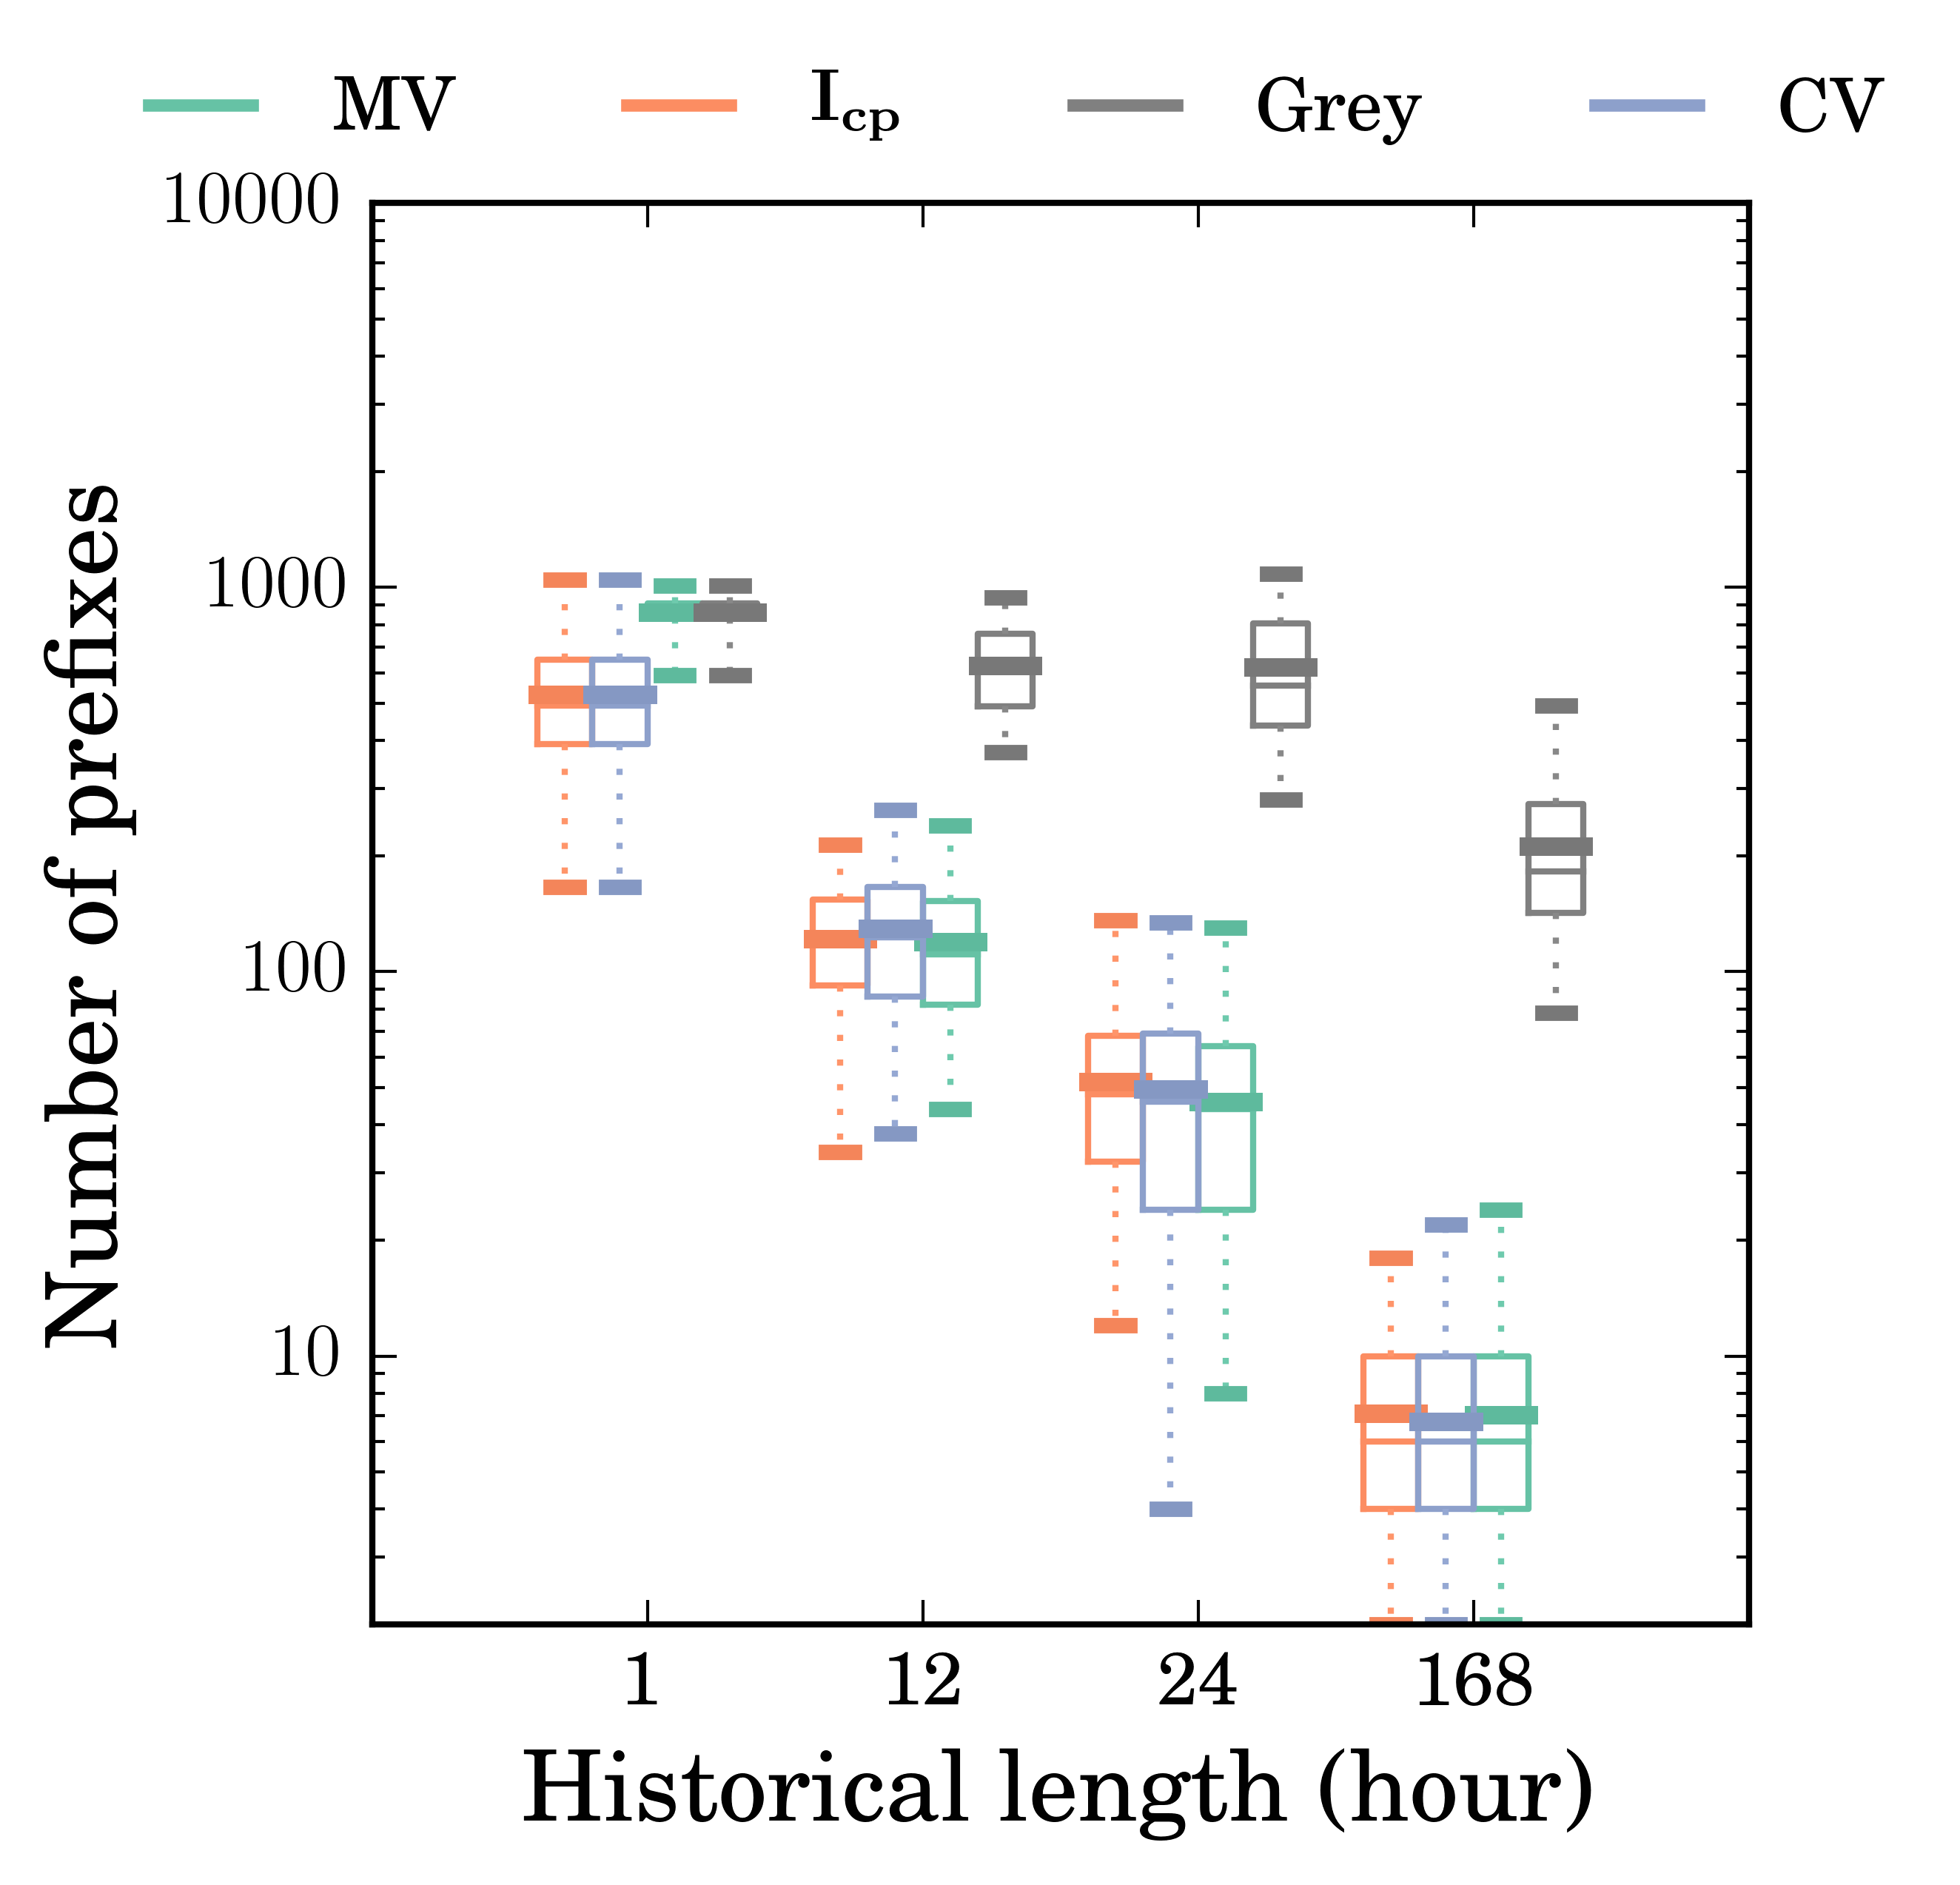
\includegraphics[width=\textwidth]{gfx/chap2/grey_churn_box_method_compare_fs_sf.png}
                \caption{SF}
                \label{fig:churn_sf}
        \end{subfigure}
\caption{Hour churn of the prefix set predictively selected using historical records of different lengths. The selection set size of each network is set to the maximum \textit{core} size over the week starting from June 1st, 2015, see in Table~\ref{tab:core_size}.}
\label{fig:churn}
\end{figure}

\begin{figure}\ContinuedFloat
	\centering 
        \begin{subfigure}[b]{0.48\textwidth}
                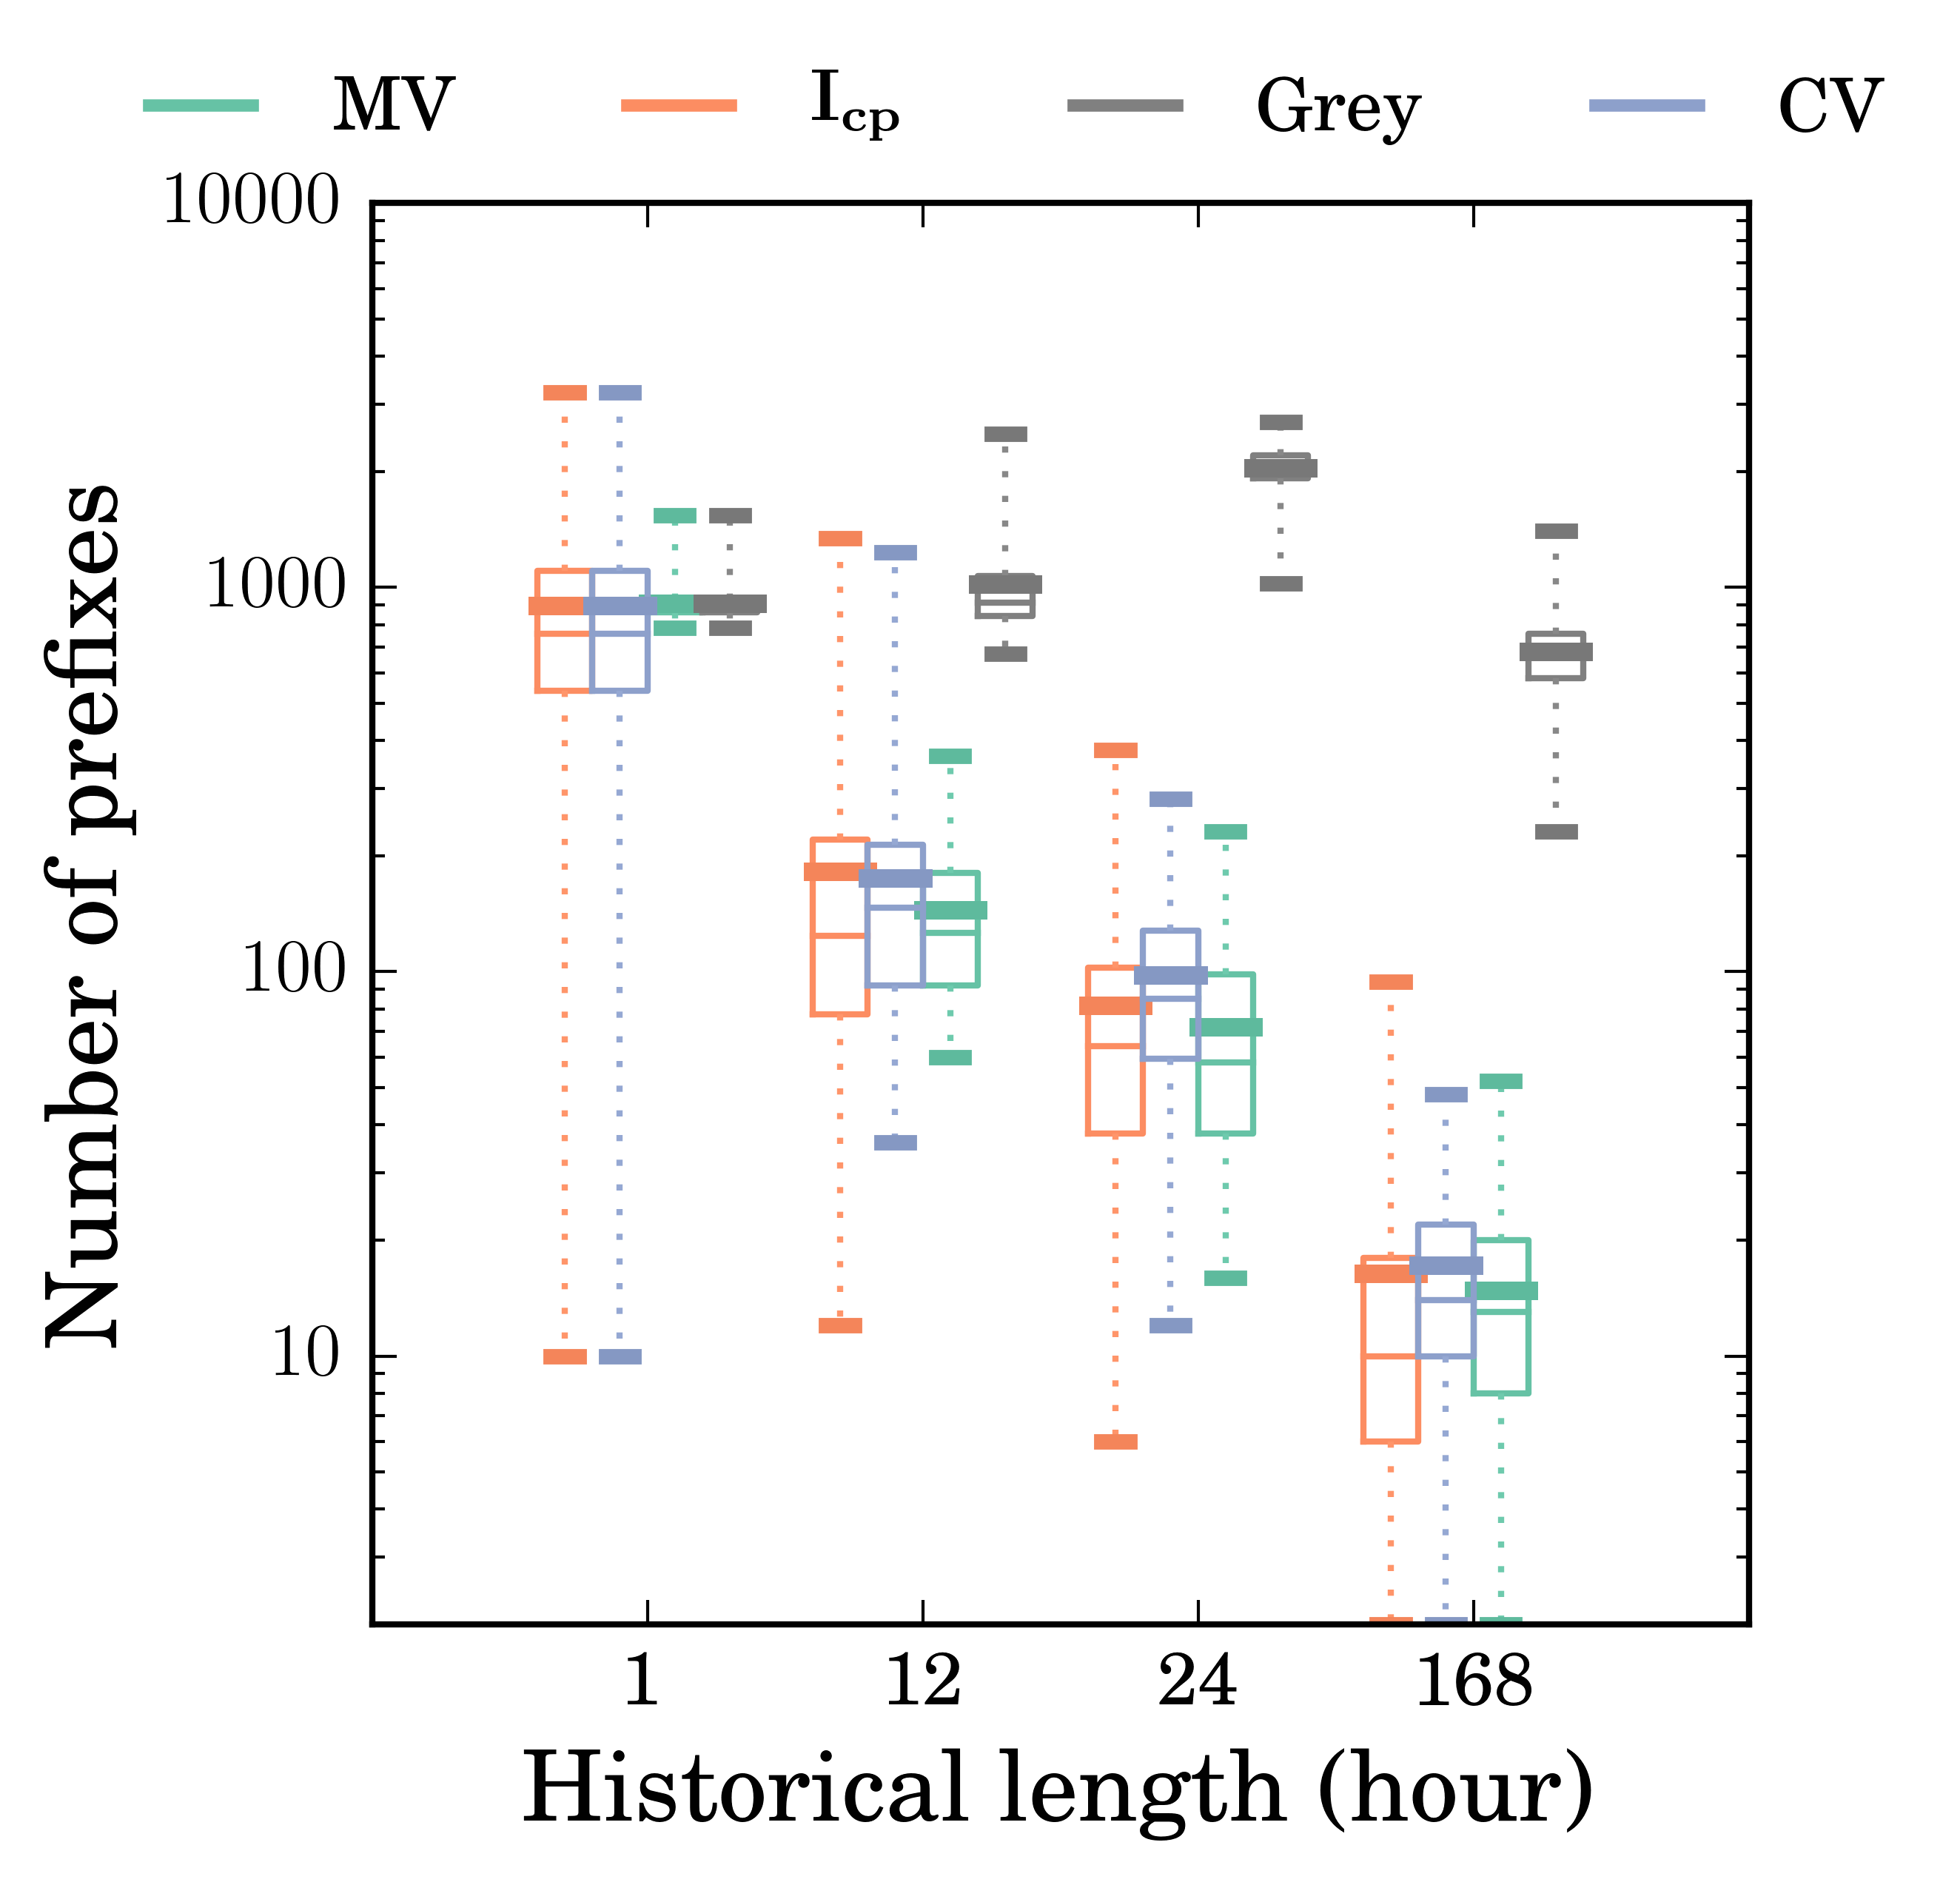
\includegraphics[width=\textwidth]{gfx/chap2/grey_churn_box_method_compare_fs_sg.png}
                \caption{SG}
                \label{fig:churn_sg}
        \end{subfigure}
        \begin{subfigure}[b]{0.48\textwidth}
                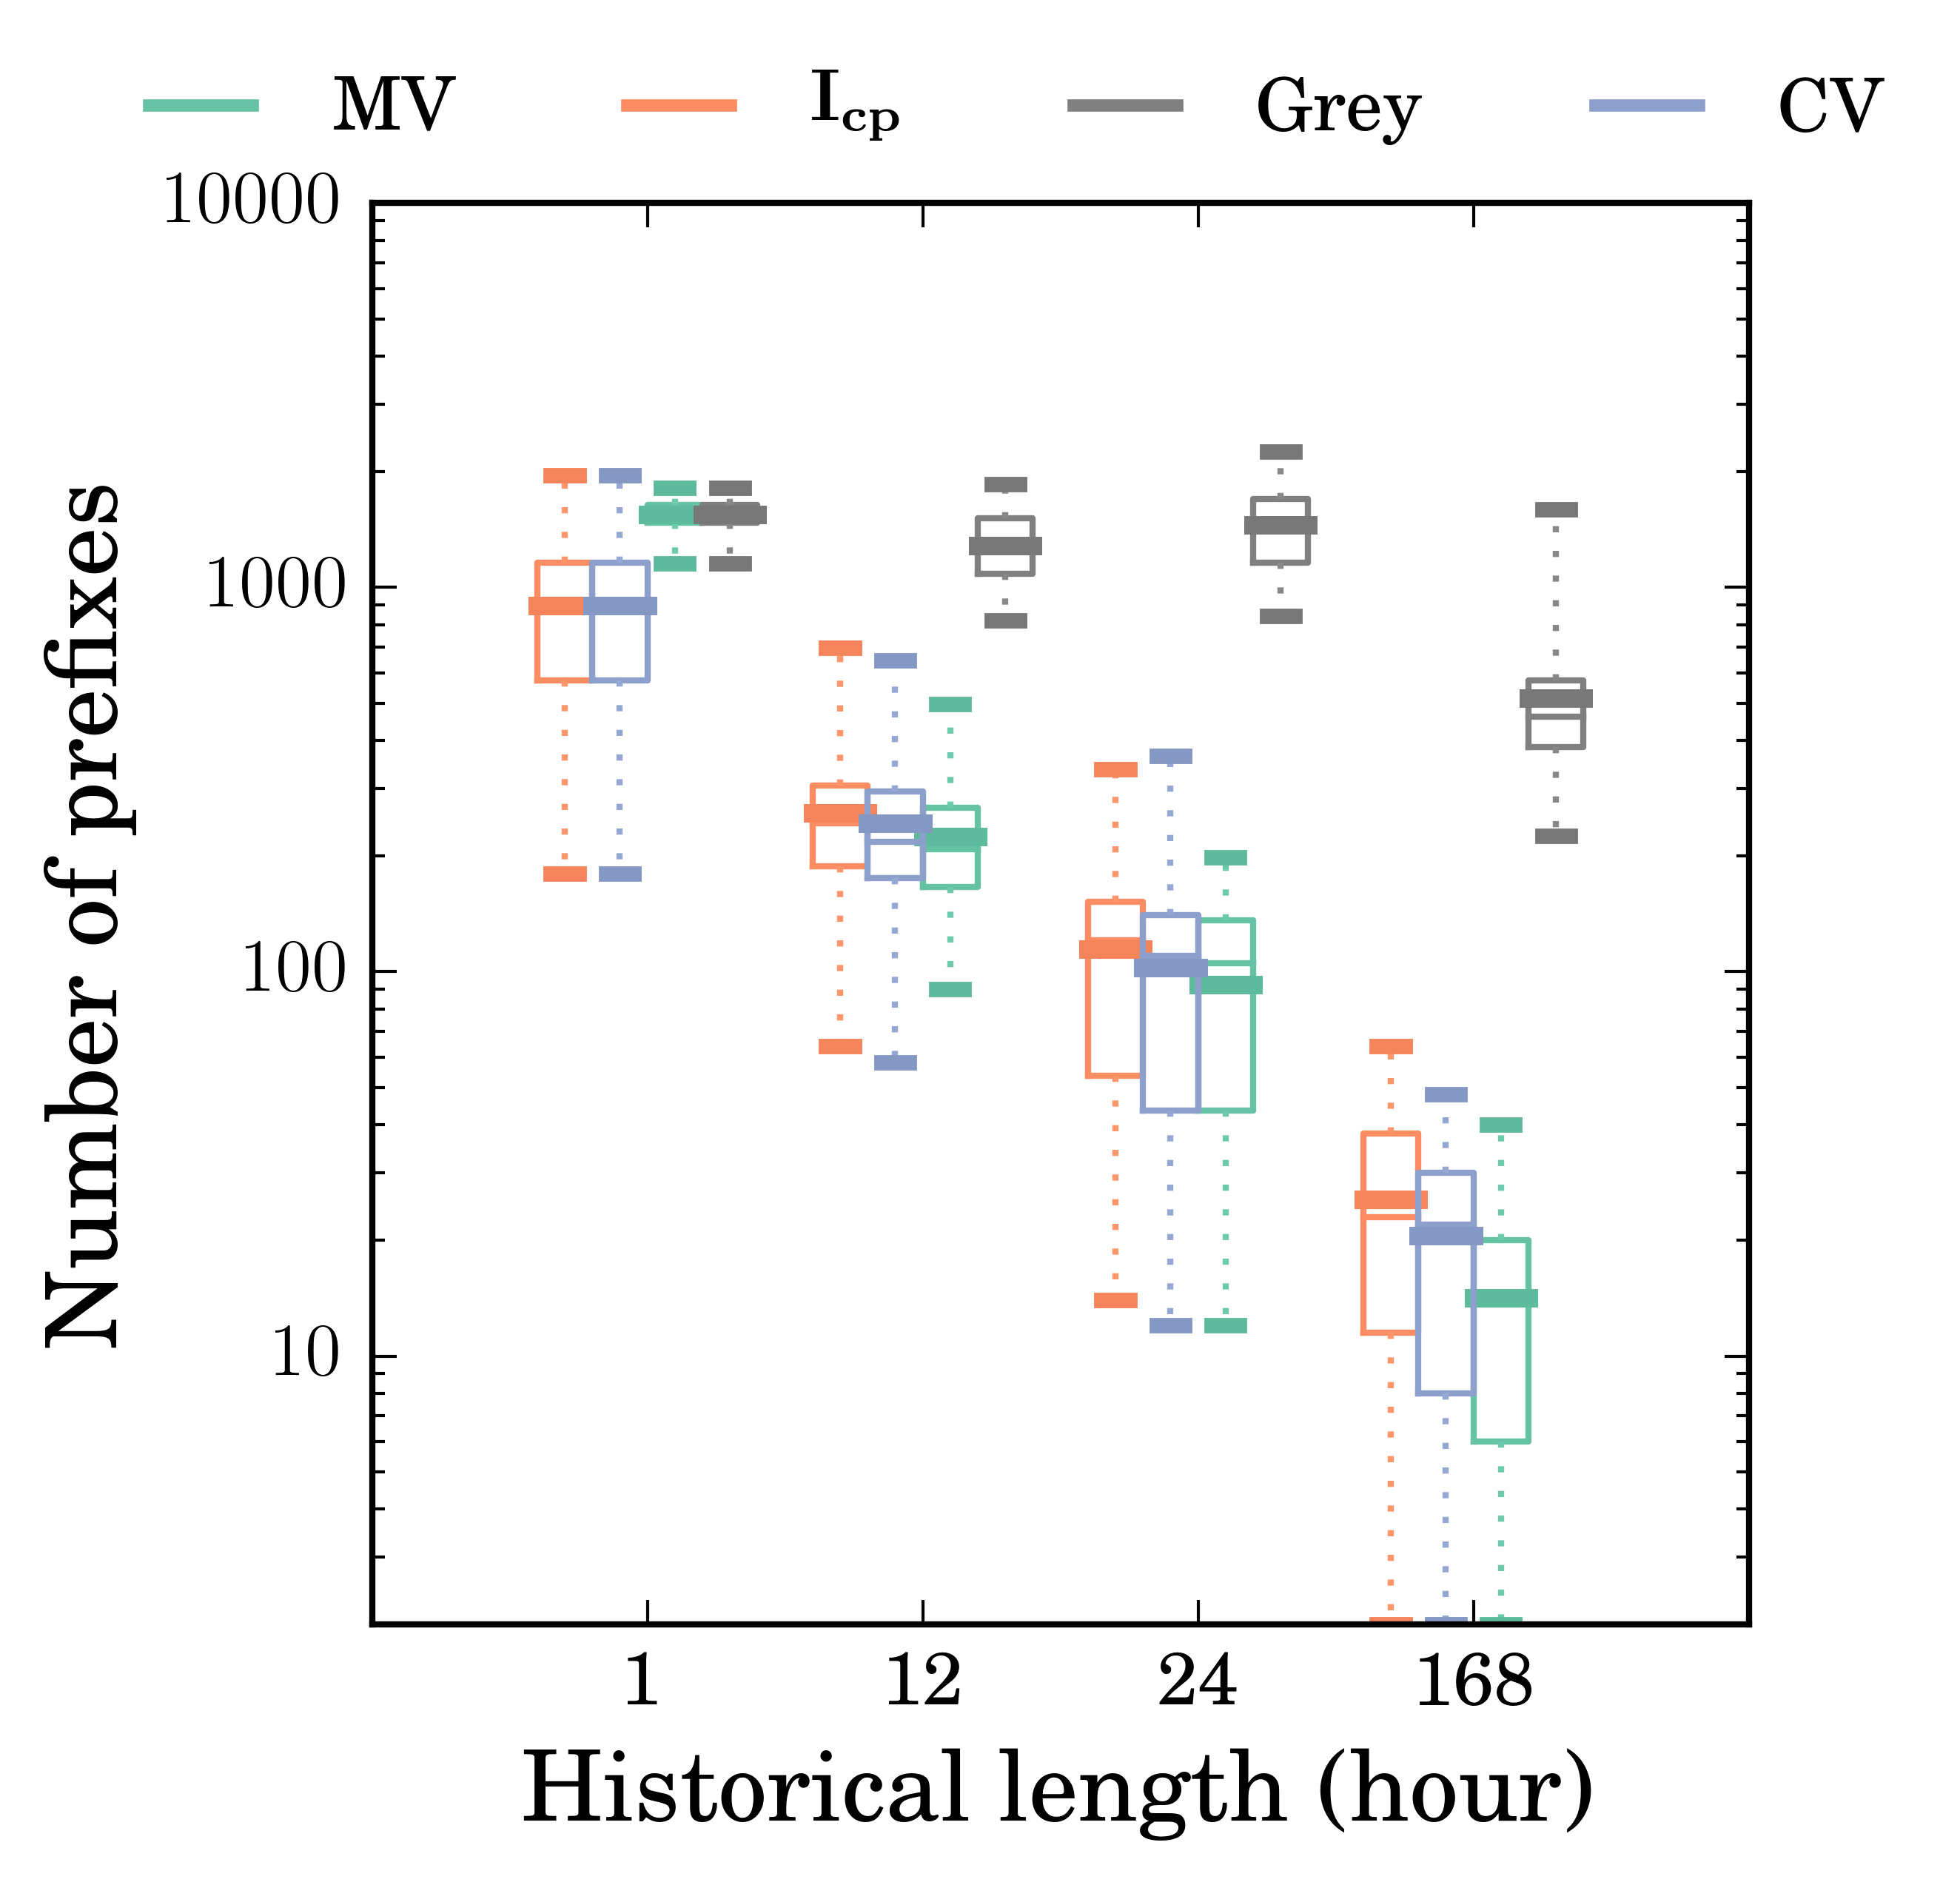
\includegraphics[width=\textwidth]{gfx/chap2/grey_churn_box_method_compare_fs_sh.png}
                \caption{SH}
                \label{fig:churn_sh}
        \end{subfigure}
        \begin{subfigure}[b]{0.48\textwidth}
                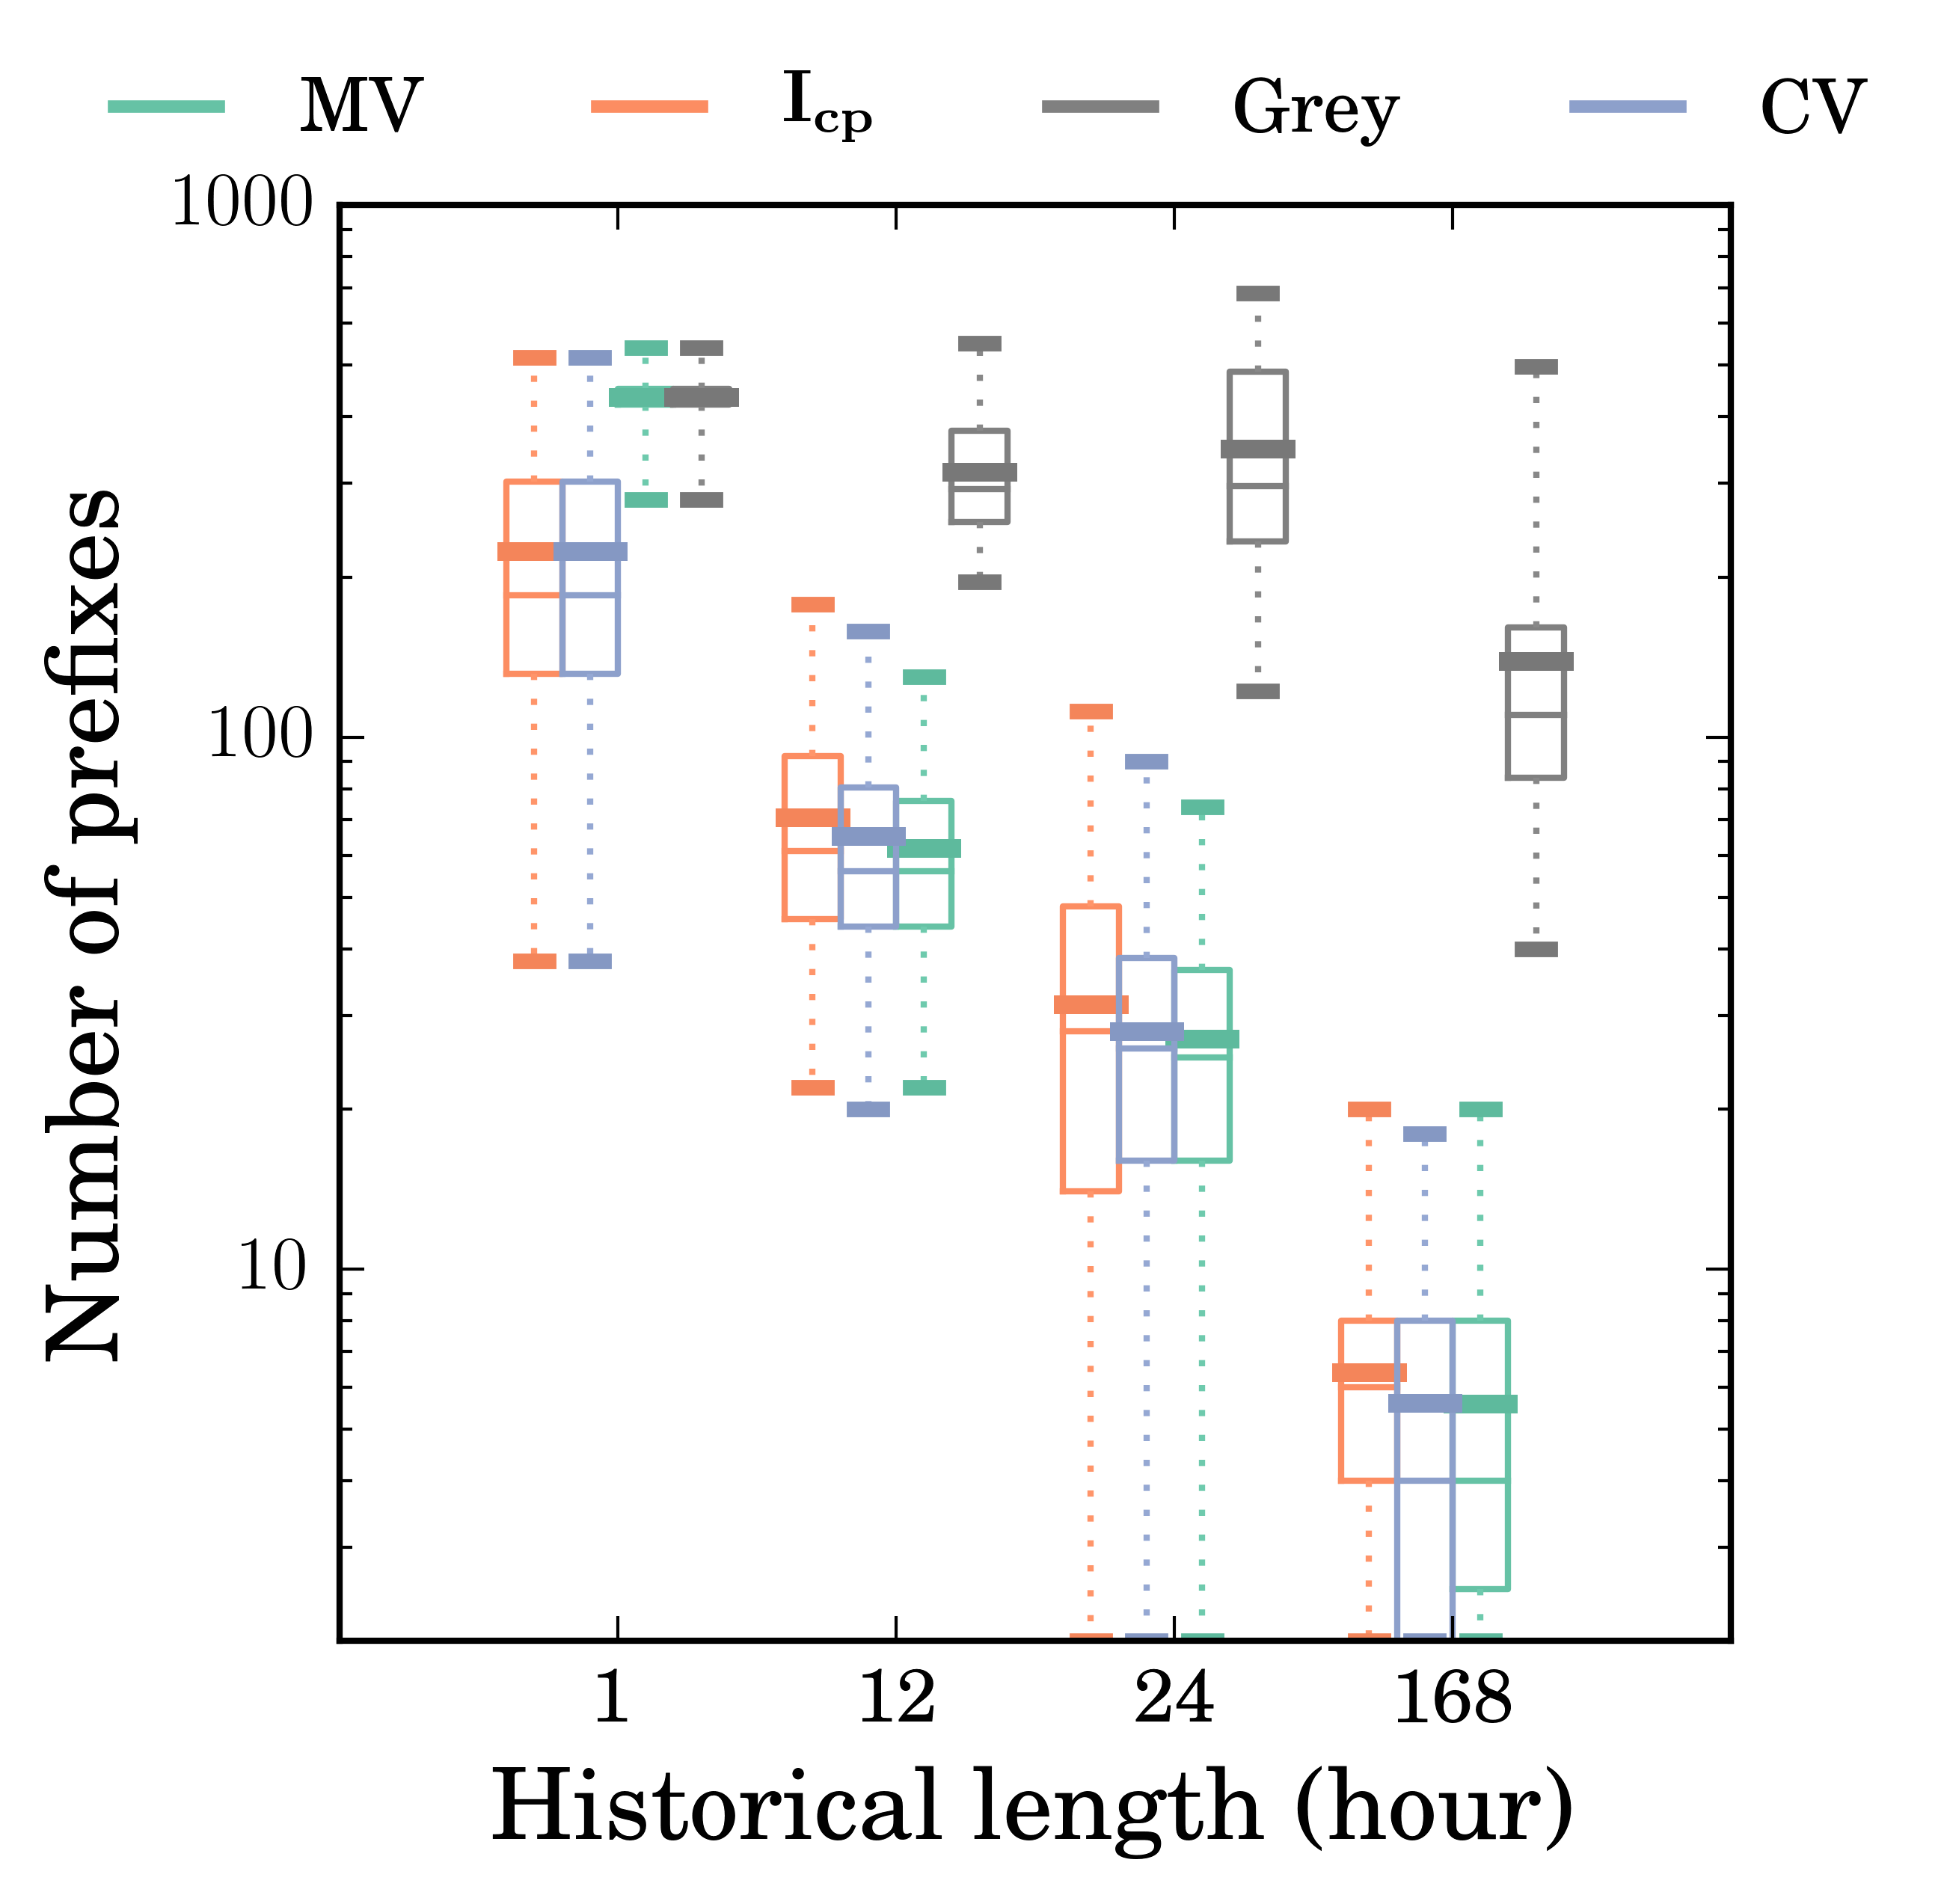
\includegraphics[width=\textwidth]{gfx/chap2/grey_churn_box_method_compare_fs_si.png}
                \caption{SI}
                \label{fig:churn_si}
        \end{subfigure}
\caption{(cont.) Hour churn of the prefix set predictively selected using historical records of different lengths.}
\label{fig:churn_cont}
\end{figure}

%\marginpar{prefix churn}
Figure~\ref{fig:churn} gives the results concerning the churn of the selection prefix set (in box-plot representation).
The churn is defined as the difference (i.e. number of new and deleted prefixes) between the new predicted set and the previous one. A high prefix churn is especially unwanted by the measurement sub-system, which aims at continuously monitoring and providing historical records of important destinations.  Sarrar et al.\ \cite{Sarrar2012} also argued that small prefix churn is very important in network architecture with decoupled forwarding and control planes, such as SDN (Software Defined Networking), for the preference over small communication overhead.

%\marginpar{discussion on historical length}
As expected, a clear drop of the churn value can be seen when the historical length increases --- as opposed to what happens with the grey model.
In that sense, using long historical records can be a wise choice in practice.
Furthermore, for networks with relatively few bursty traffic, e.g. SA, the mean volume coverage with last 168 hour records is extremely close to that with last 24 hour records, shown in Figure~\ref{fig:cvg_sa}.
Finally, for networks with highly bursty traffic, SC, using long records has the potential to obviously improve worst-case volume coverage. 

For the purpose of lowering churn, Sarrar et al.\ \cite{Sarrar2012} proposed selecting top prefixes over time bins of different lengths (ranging from 1 second to 10 minute in their FIB-caching environment). In our context, we found that the difference in mean volume coverage using record lengths larger than 1 hour is marginal, thus little gain can be expected from this method.  

%\begin{table*}[!htb]
%\centering
%\begin{tabular}{cc|cc|cc}\toprule
%\textbf{Network} & \textbf{$L$}  & \textbf{Mean Cvg.} & \textbf{Min Cvg.} & \textbf{Mean Churn} & %\textbf{Max Churn}\\
%\midrule
%SA & 24   & 93.73 & 85.32 & 32.23  & 148\\
%SB & 24   & 88.02 & 79.82 & 873.11 & 4026\\
%SC & 168  & 88.73 & 61.11 & 2.84   & 10\\
%SD & 168  & 83.22 & 69.23 & 107.06 & 1642\\
%SE & 24   & 90.51 & 78.85 & 613.72 & 1664 \\
%SF & 24   & 81.33 & 51.94 & 49.52  & 134\\
%SG & 168  & 86.44 & 52.60 & 17.24  & 48\\
%SH & 24   & 92.04 & 81.21 & 102.60 & 364\\
%SI & 24   & 87.71 & 66.75 & 28.01  & 90\\
%\bottomrule
%\end{tabular}
%\caption{Hourly volume coverage (in percentage) and churn, using \text{core} volume metric $CV$ with record length $L$ yielding the highest mean coverage.}
%\label{tab:cvg_churn}
%\end{table*}

%Among all the networks, we achieved the best mean volume coverage under $CV$ metric ($>92\%$) on SA and SH, as it can seen in Table~\ref{tab:cvg_churn}. 
%This corresponds to the fact that these two networks suffers the lest from bursty traffic.

\subsubsection{Relation between volume coverage and traffic burstiness}

\begin{figure}[!tb]
\centering
		\centering
        \begin{subfigure}[b]{0.42\textwidth}
        \centering
                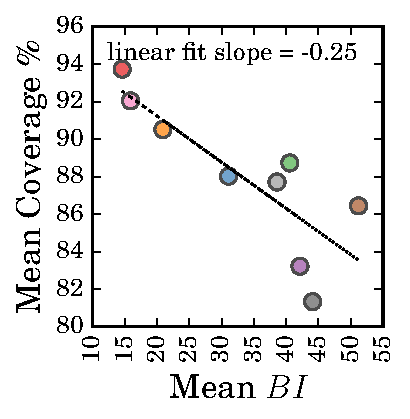
\includegraphics[width=\textwidth]{gfx/chap2/bi_cvg_mean.pdf}
                \caption{Average level}
                \label{fig:bi_cvg_mean}
        \end{subfigure}
        \hfill
        \begin{subfigure}[b]{0.53\textwidth}
                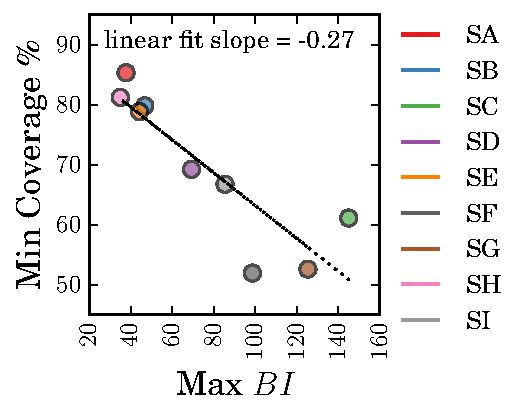
\includegraphics[width=\textwidth]{gfx/chap2/bi_cvg_worst.pdf}
                \caption{Worst case}
                \label{fig:bi_cvg_worst}
        \end{subfigure}
\caption{The relationship between burstiness index $BI$ and traffic volume coverage of selected prefix using $CV$ metric.}
\label{fig:bi_cvg}
\end{figure}

The mean/minimum coverage achieved with $CV$ metric is showed as a function of the $BI$ index in Figure~\ref{fig:bi_cvg}. 
We can see that the mean (resp. minimum) coverage is inversely proportional to the mean (resp. maximum) $BI$ index. 
This relation highlights the difficulty to cover a big fraction of traffic volume for networks with more bursty traffic. 
However, the quasi-linear curve obtained shows that $BI$ is a very meaningful metric to identify sites with bursty trafic. 
For network with large $BI$ values, it is worthy of choosing a larger prefix set size (which was previously fixed to the weekly maximum core size), if possible. 

\section{Transit provider performance evaluation}
\label{sec:rtt}

\begin{figure}
\centering
		\centering
        \begin{subfigure}[b]{0.48\textwidth}
                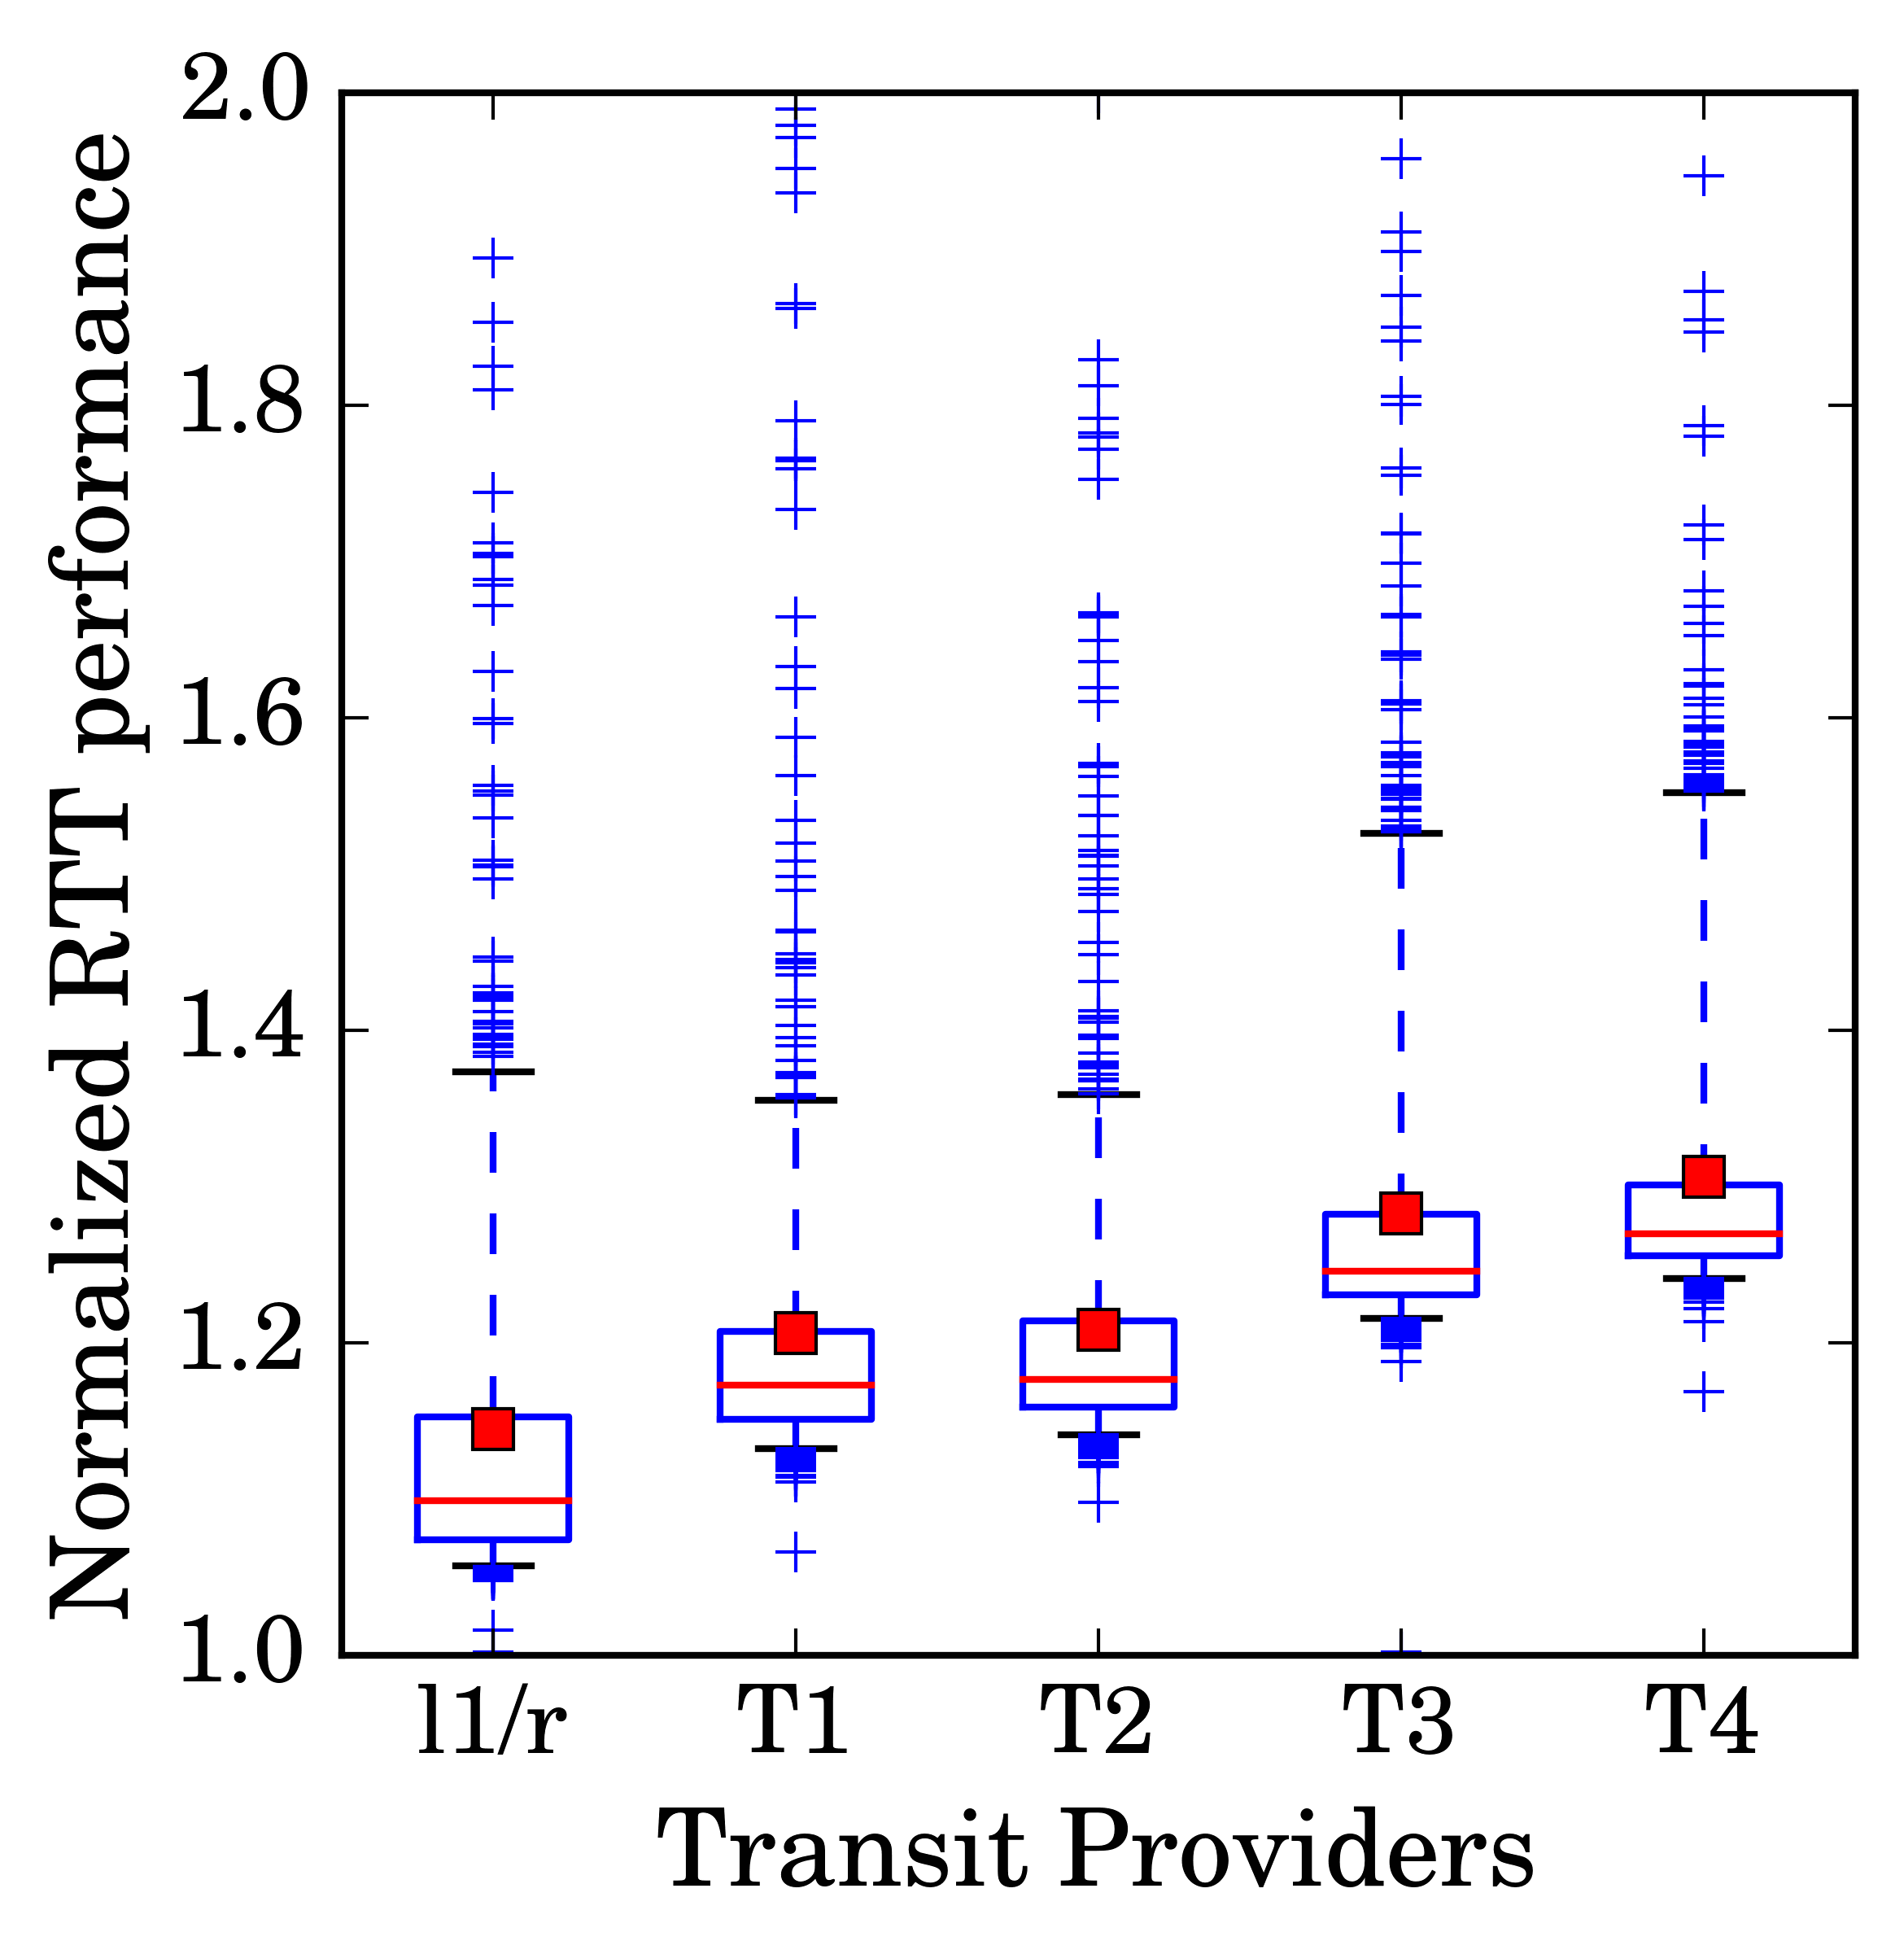
\includegraphics[width=\textwidth]{gfx/chap2/np_box_sa.png}
                \caption{SA, 866 prefixes, $85.69\%$ traffic}
                \label{fig:np_sa}
        \end{subfigure}
        \begin{subfigure}[b]{0.48\textwidth}
                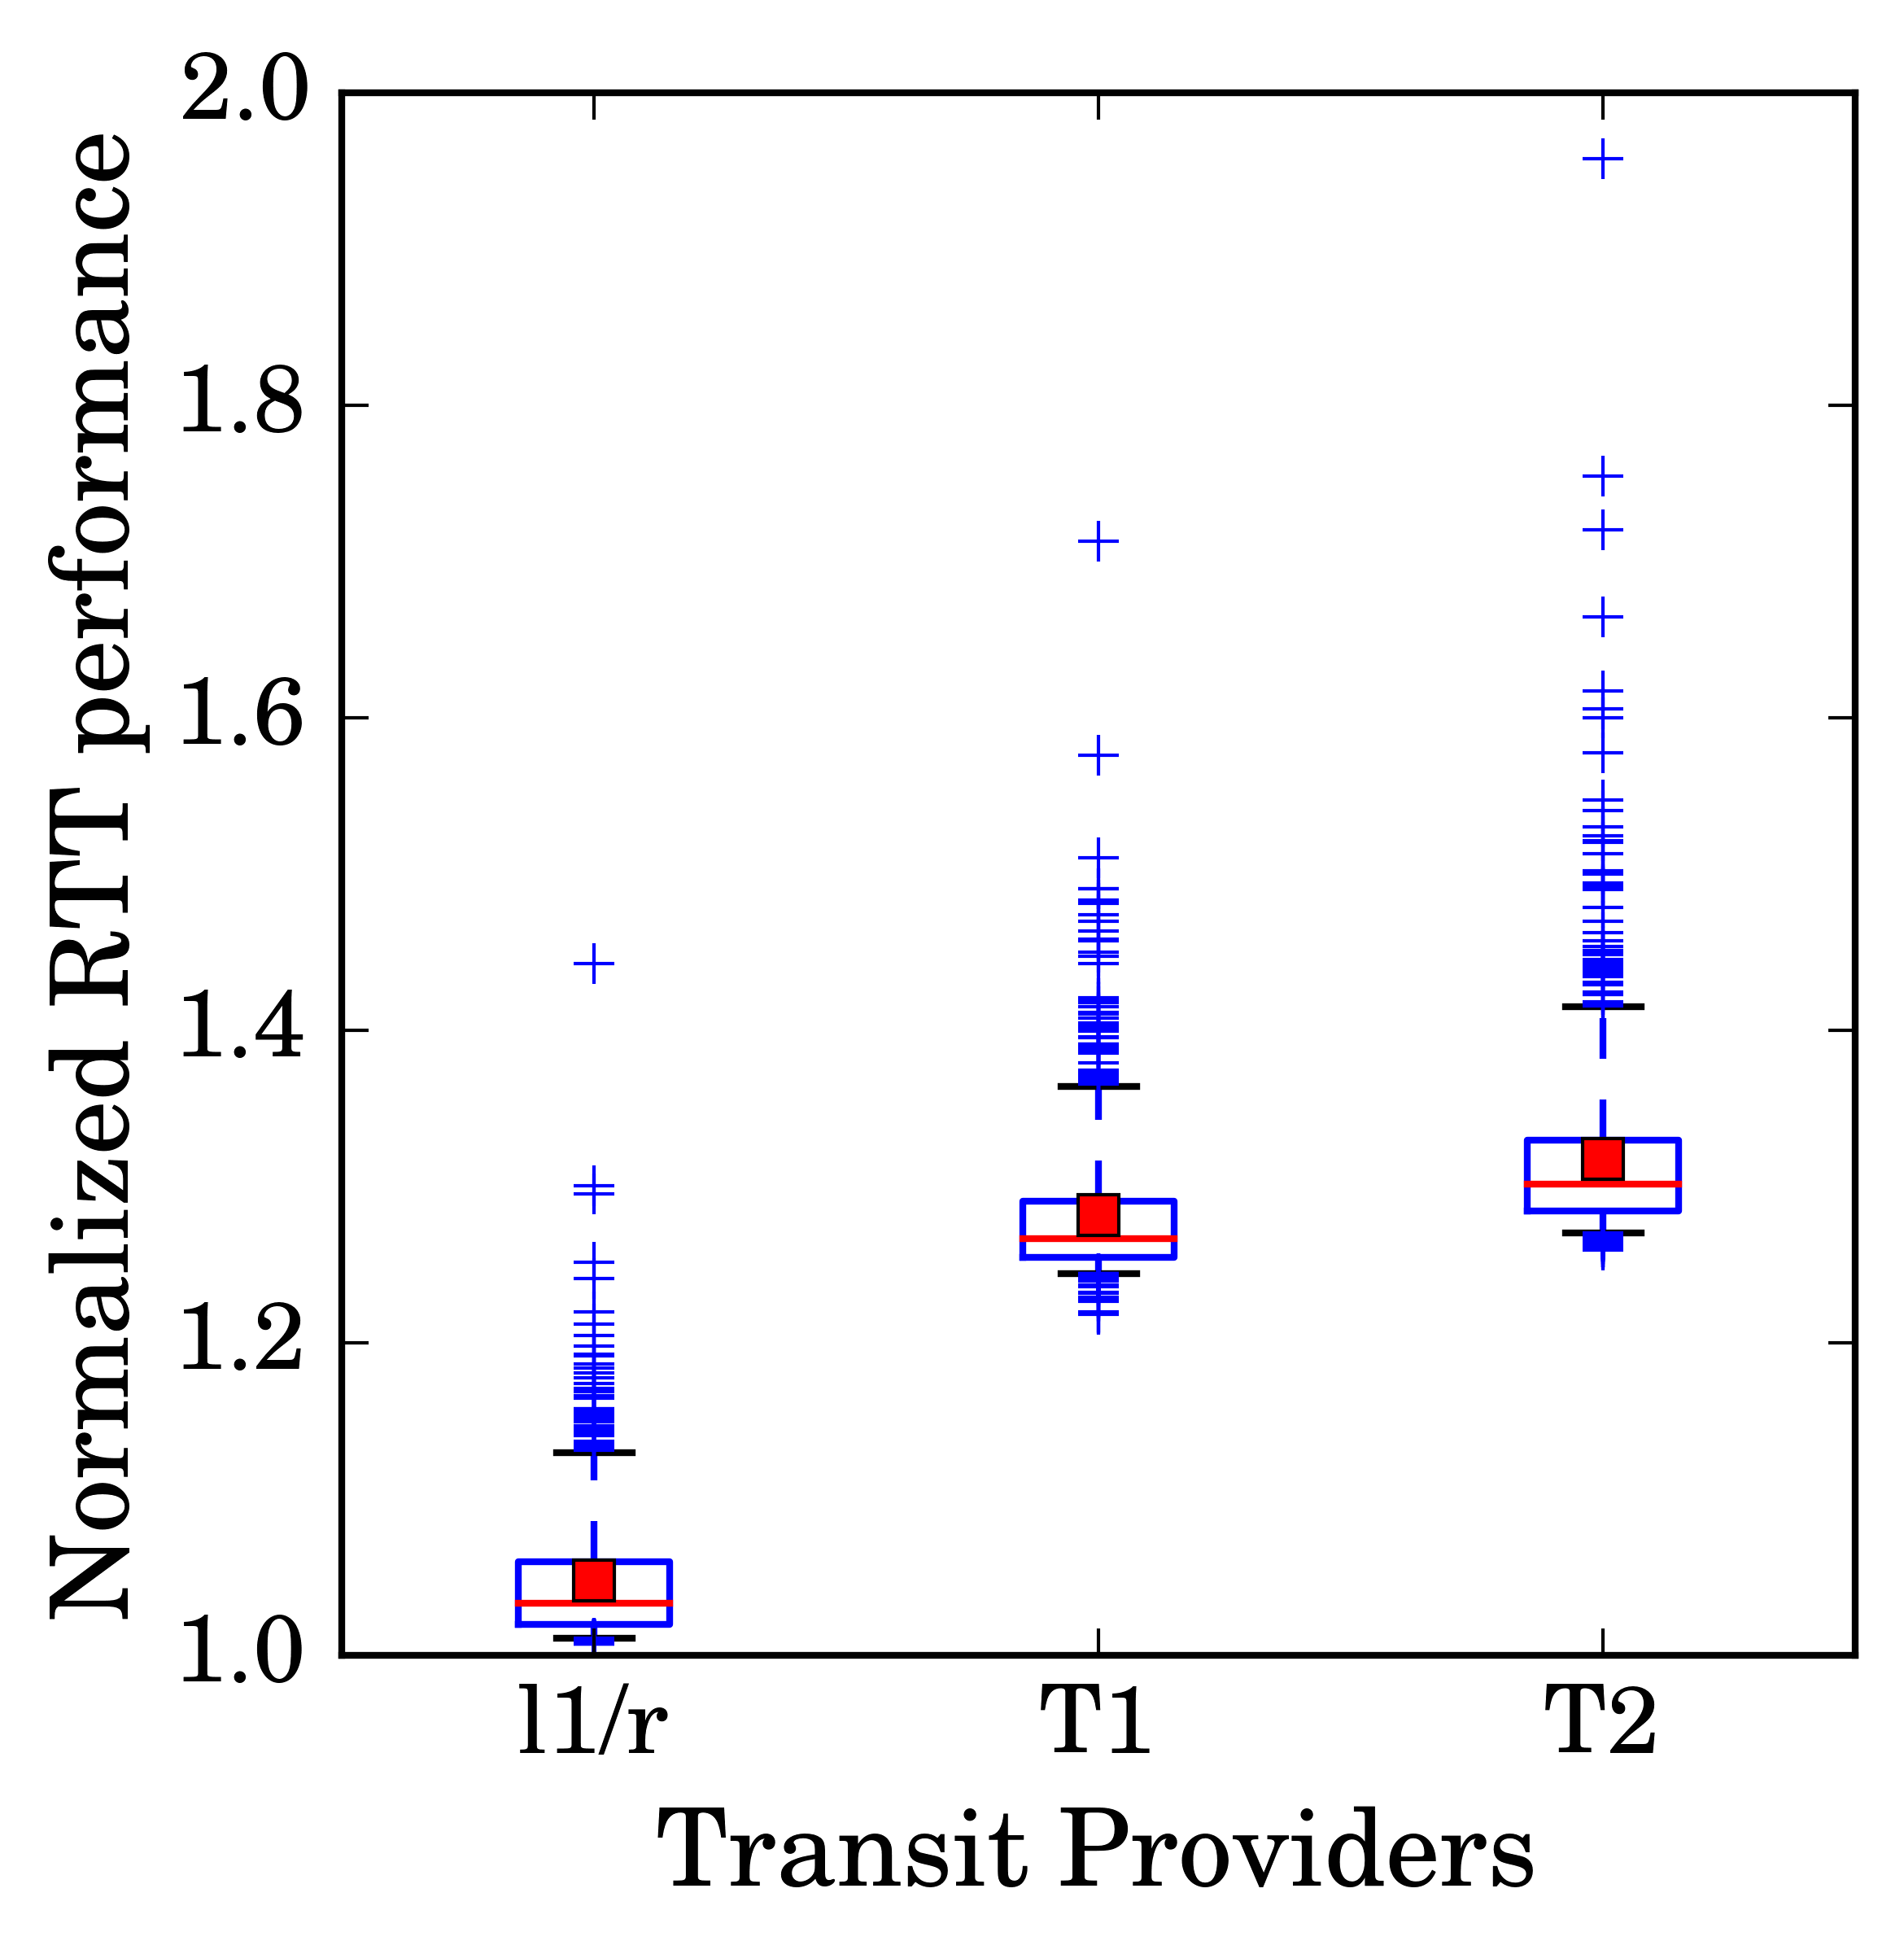
\includegraphics[width=\textwidth]{gfx/chap2/np_box_sb.png}
                \caption{SB, 935 prefixes, $48.49\%$ traffic}
                \label{fig:np_sb}
        \end{subfigure}
        \begin{subfigure}[b]{0.48\textwidth}
                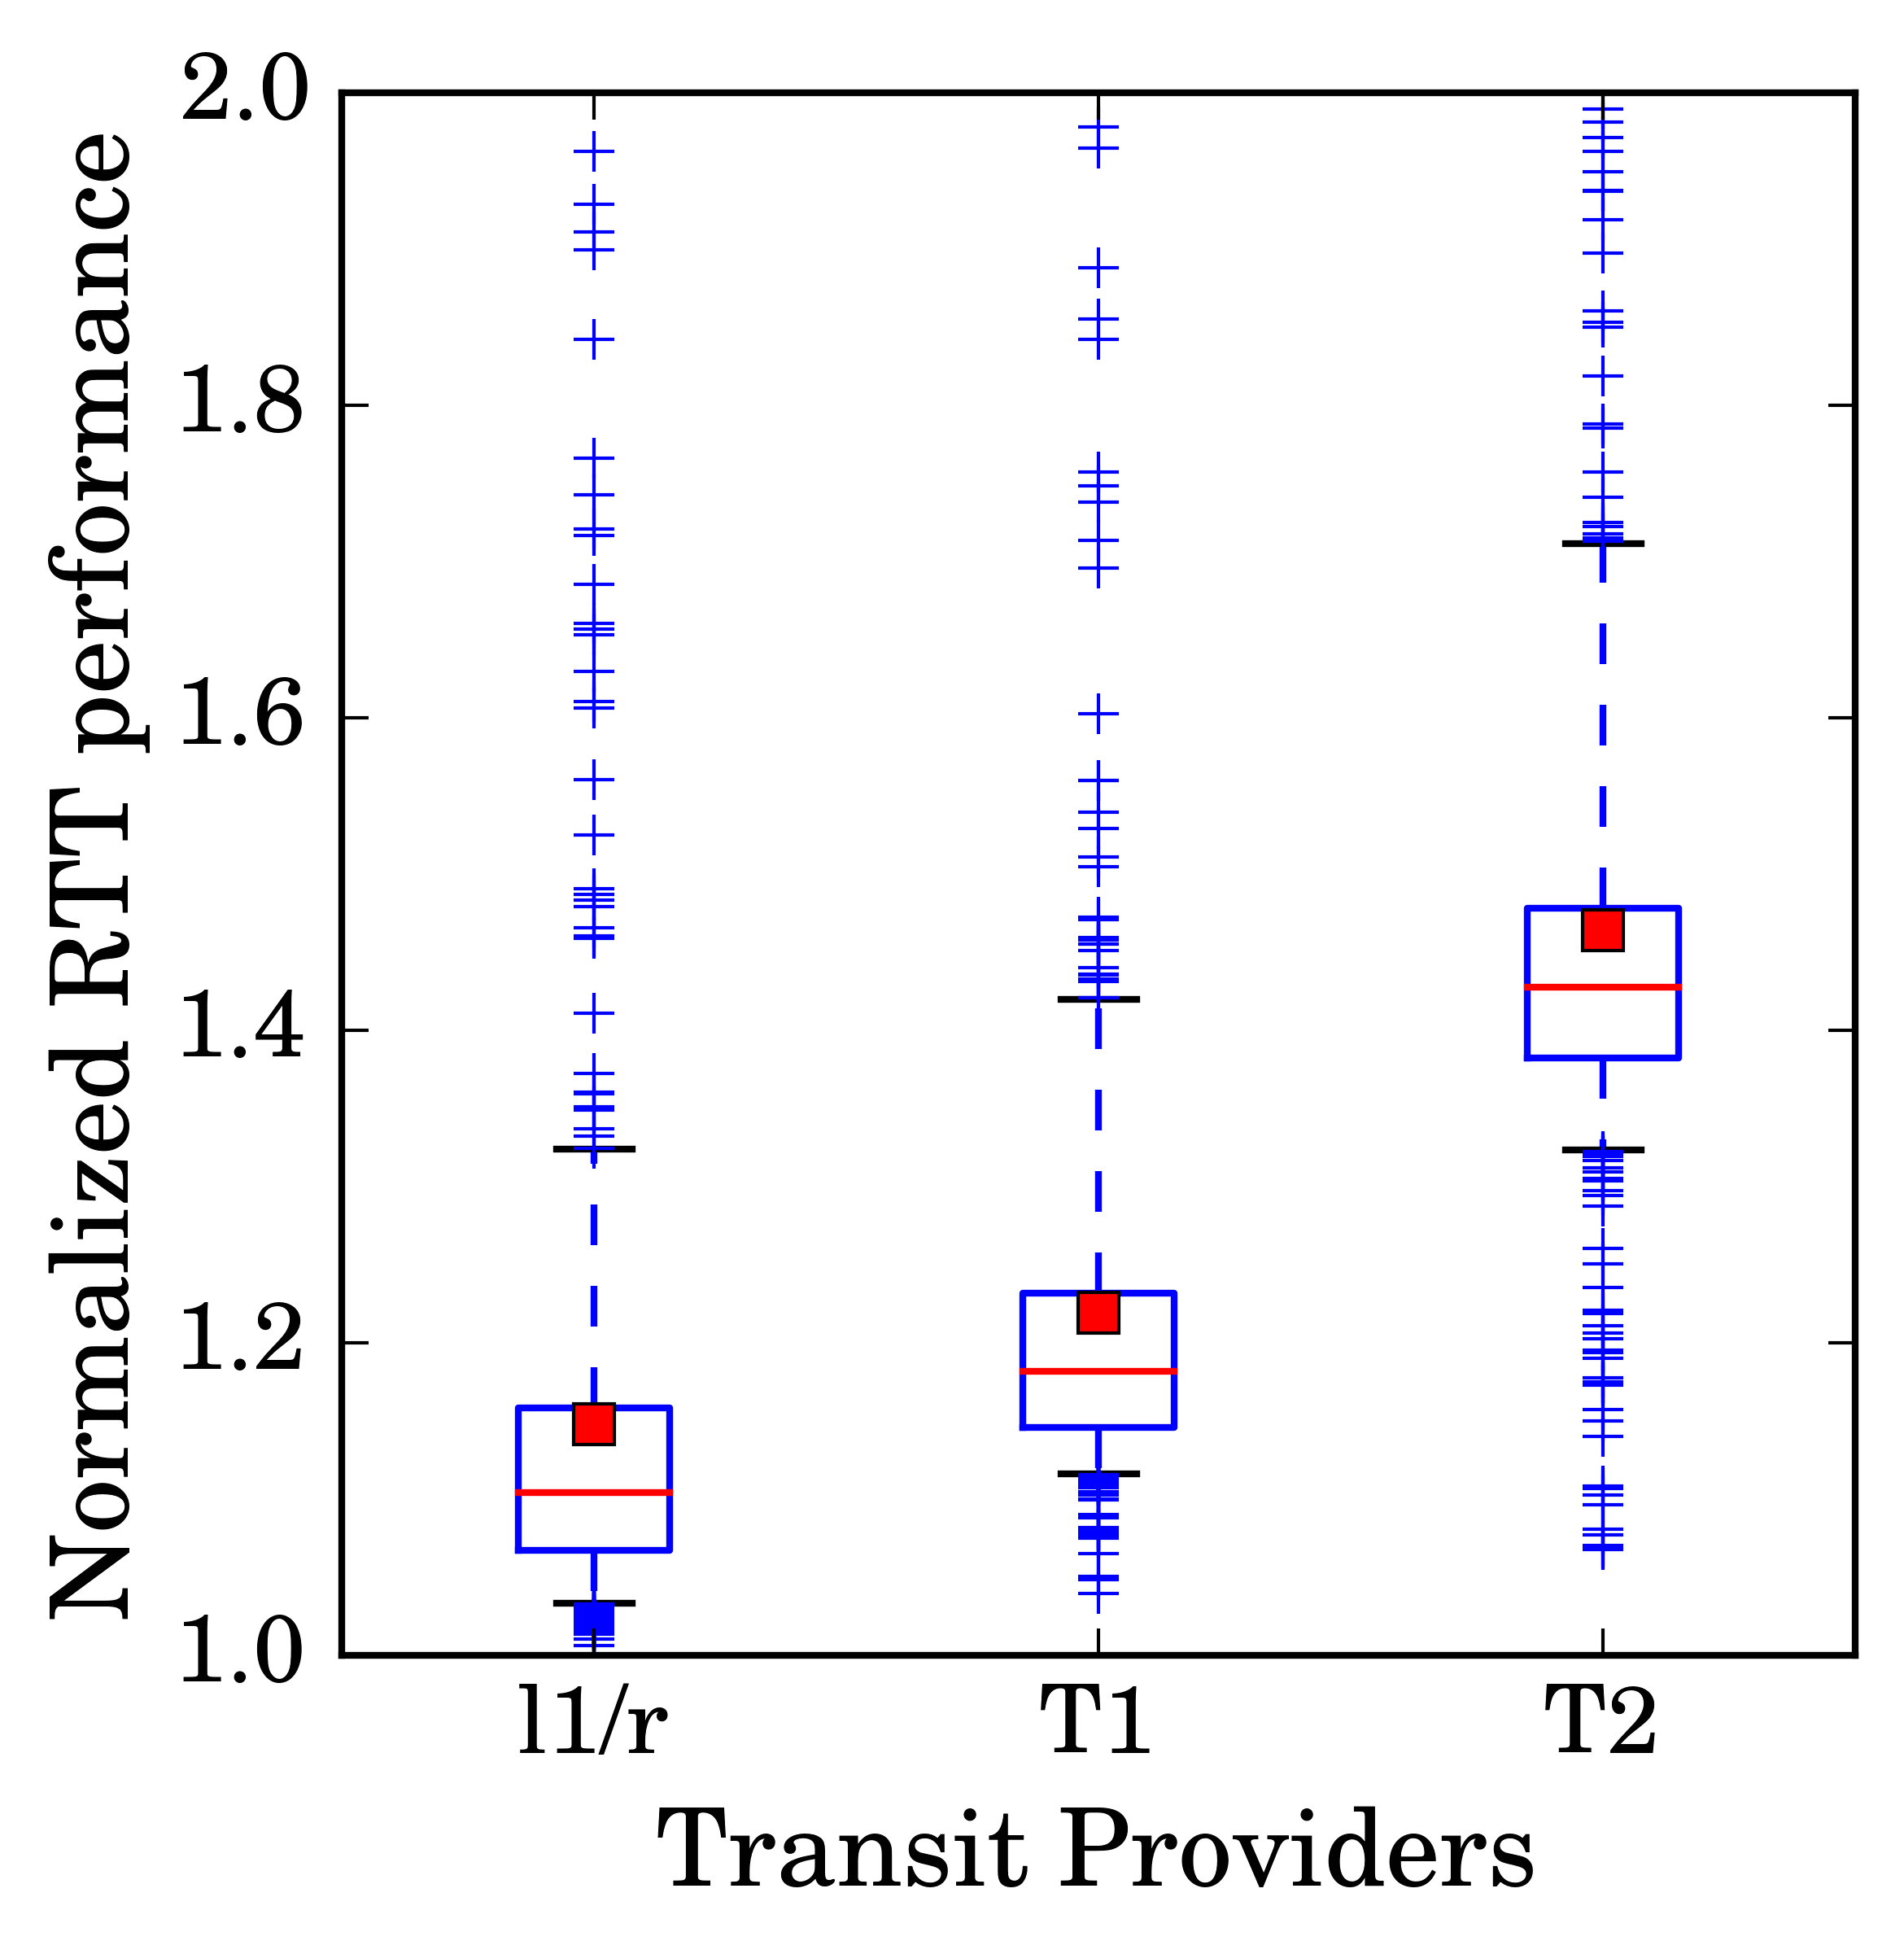
\includegraphics[width=\textwidth]{gfx/chap2/np_box_sc.png}
                \caption{SC, 762 prefixes, $44.23\%$ traffic}
                \label{fig:np_sc}
        \end{subfigure}
        \begin{subfigure}[b]{0.48\textwidth}
                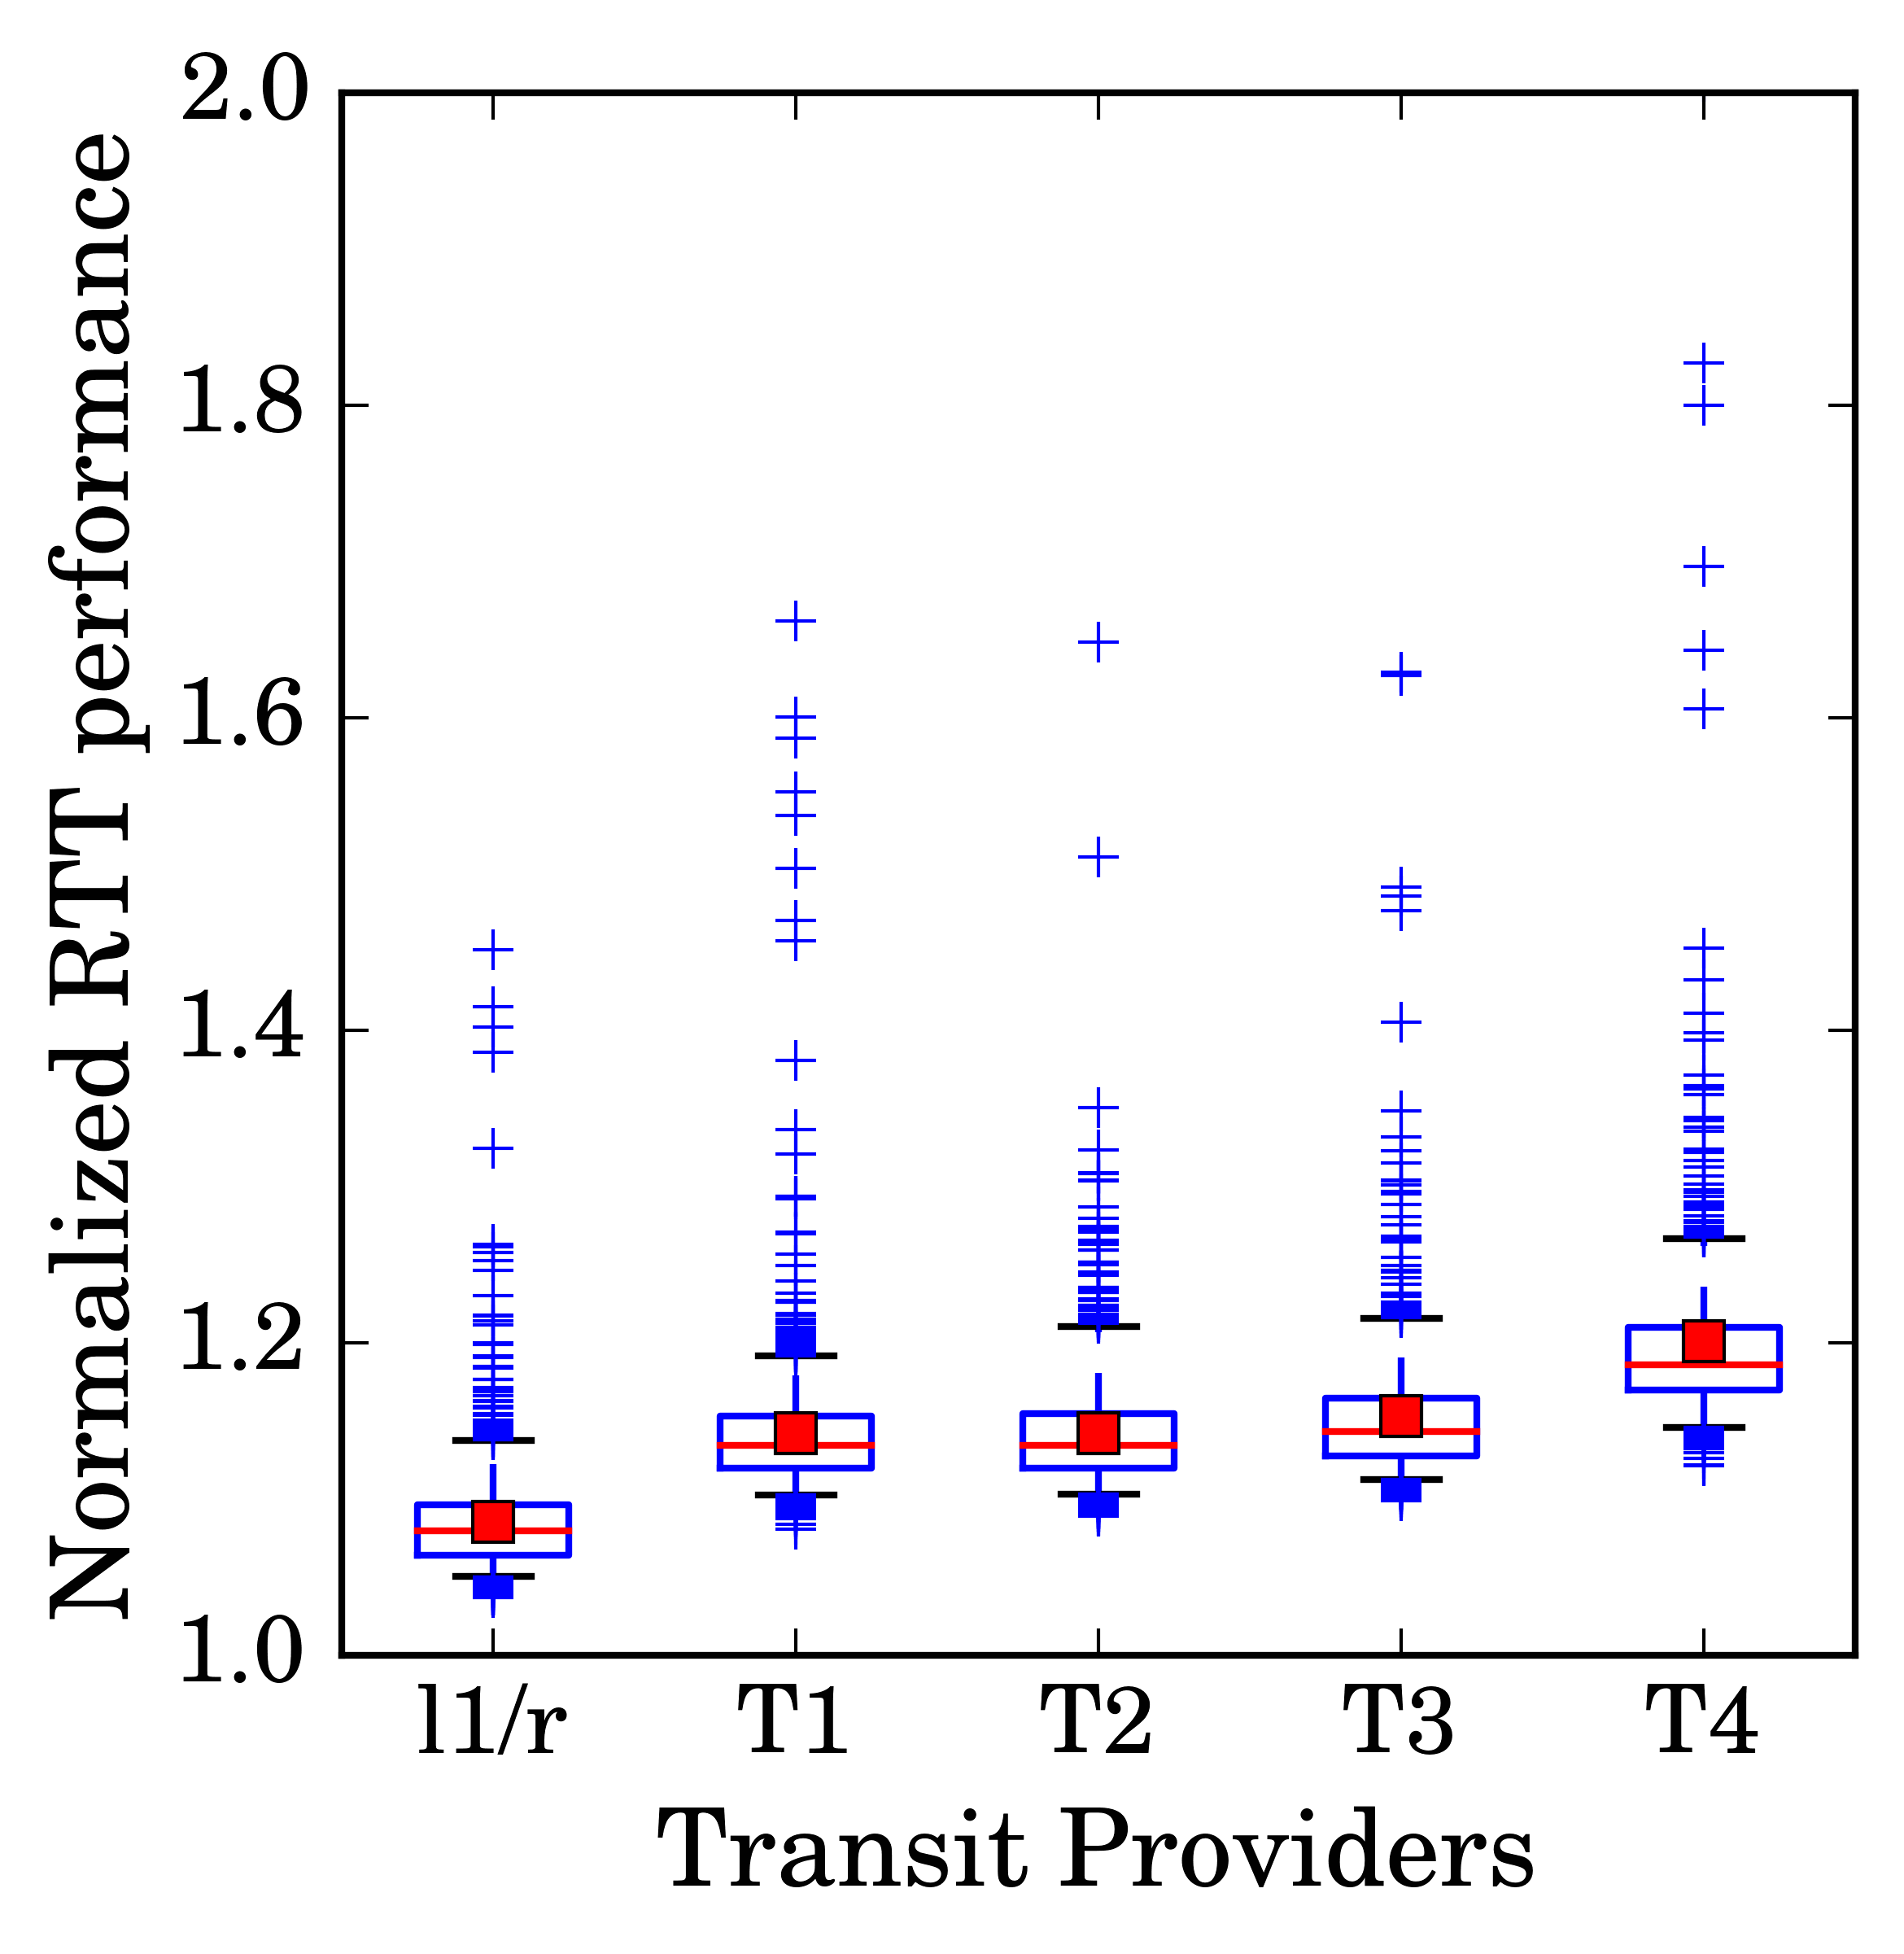
\includegraphics[width=\textwidth]{gfx/chap2/np_box_sd.png}
                \caption{SD, 2841 prefixes, $49.18\%$ traffic}
                \label{fig:np_sd}
        \end{subfigure}
        \begin{subfigure}[b]{0.48\textwidth}
                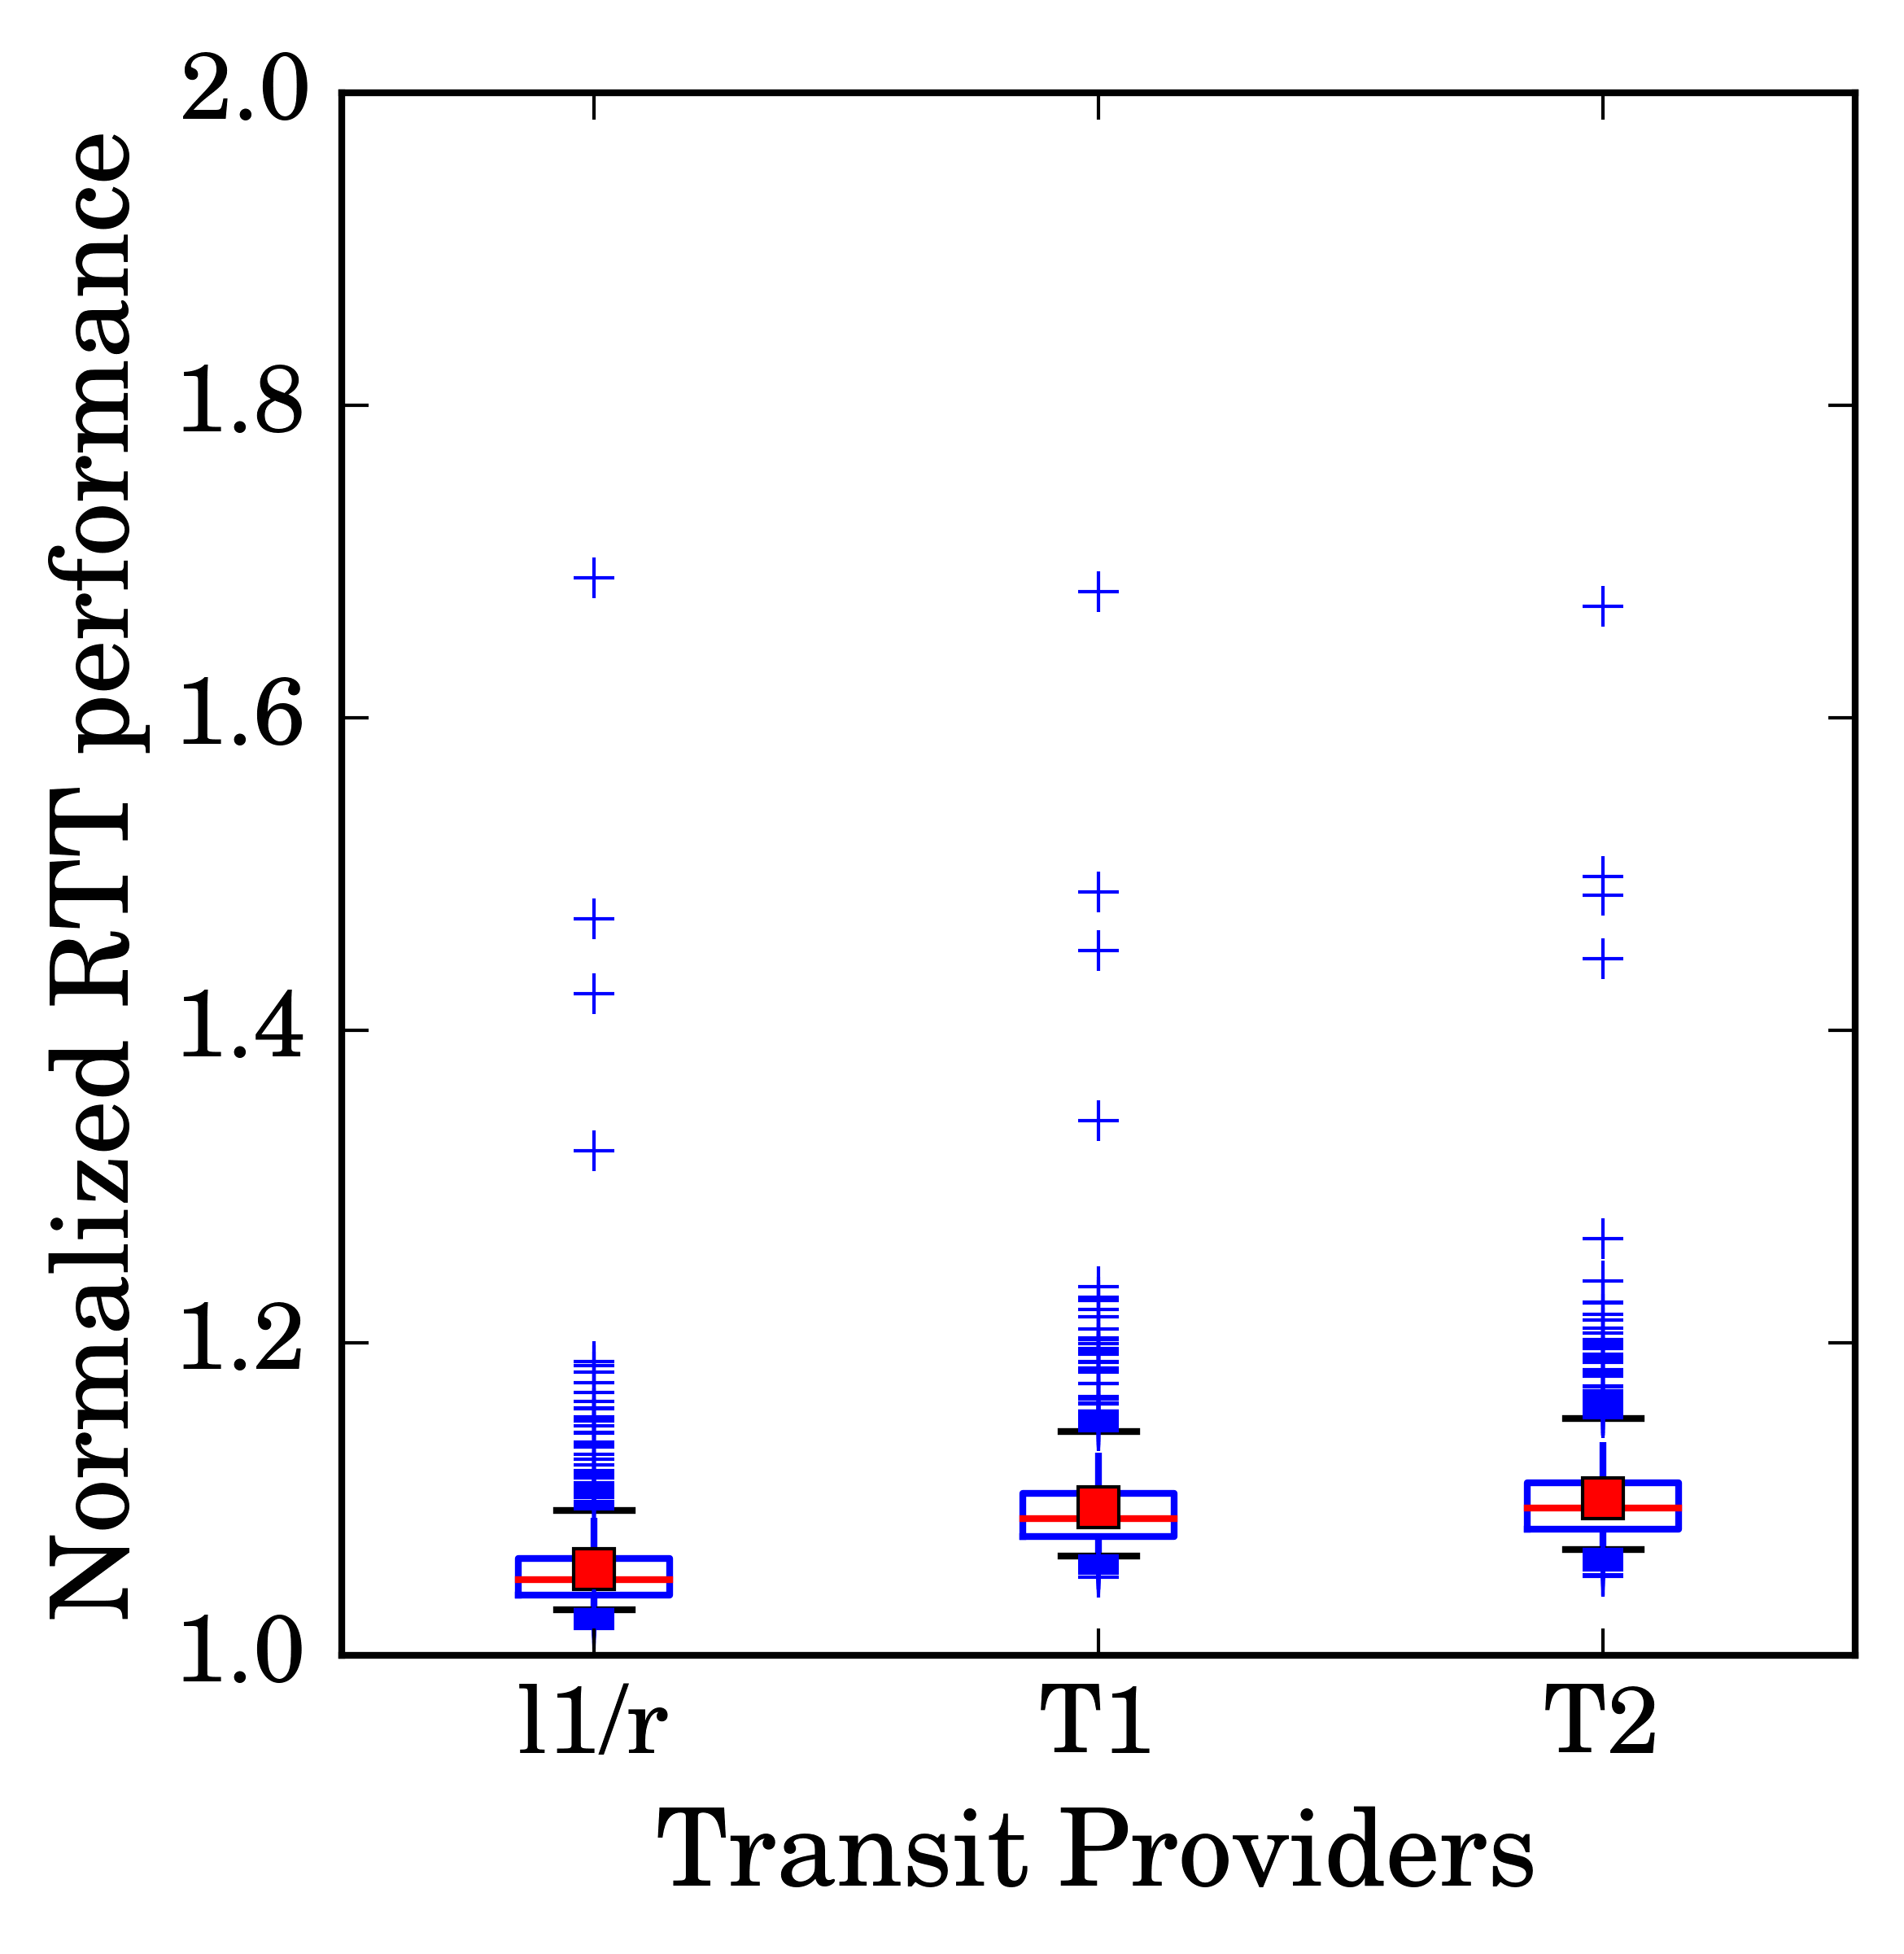
\includegraphics[width=\textwidth]{gfx/chap2/np_box_se.png}
                \caption{SE, 2287 prefixes, $38.59\%$ traffic}
                \label{fig:np_se}
        \end{subfigure}
        \begin{subfigure}[b]{0.48\textwidth}
                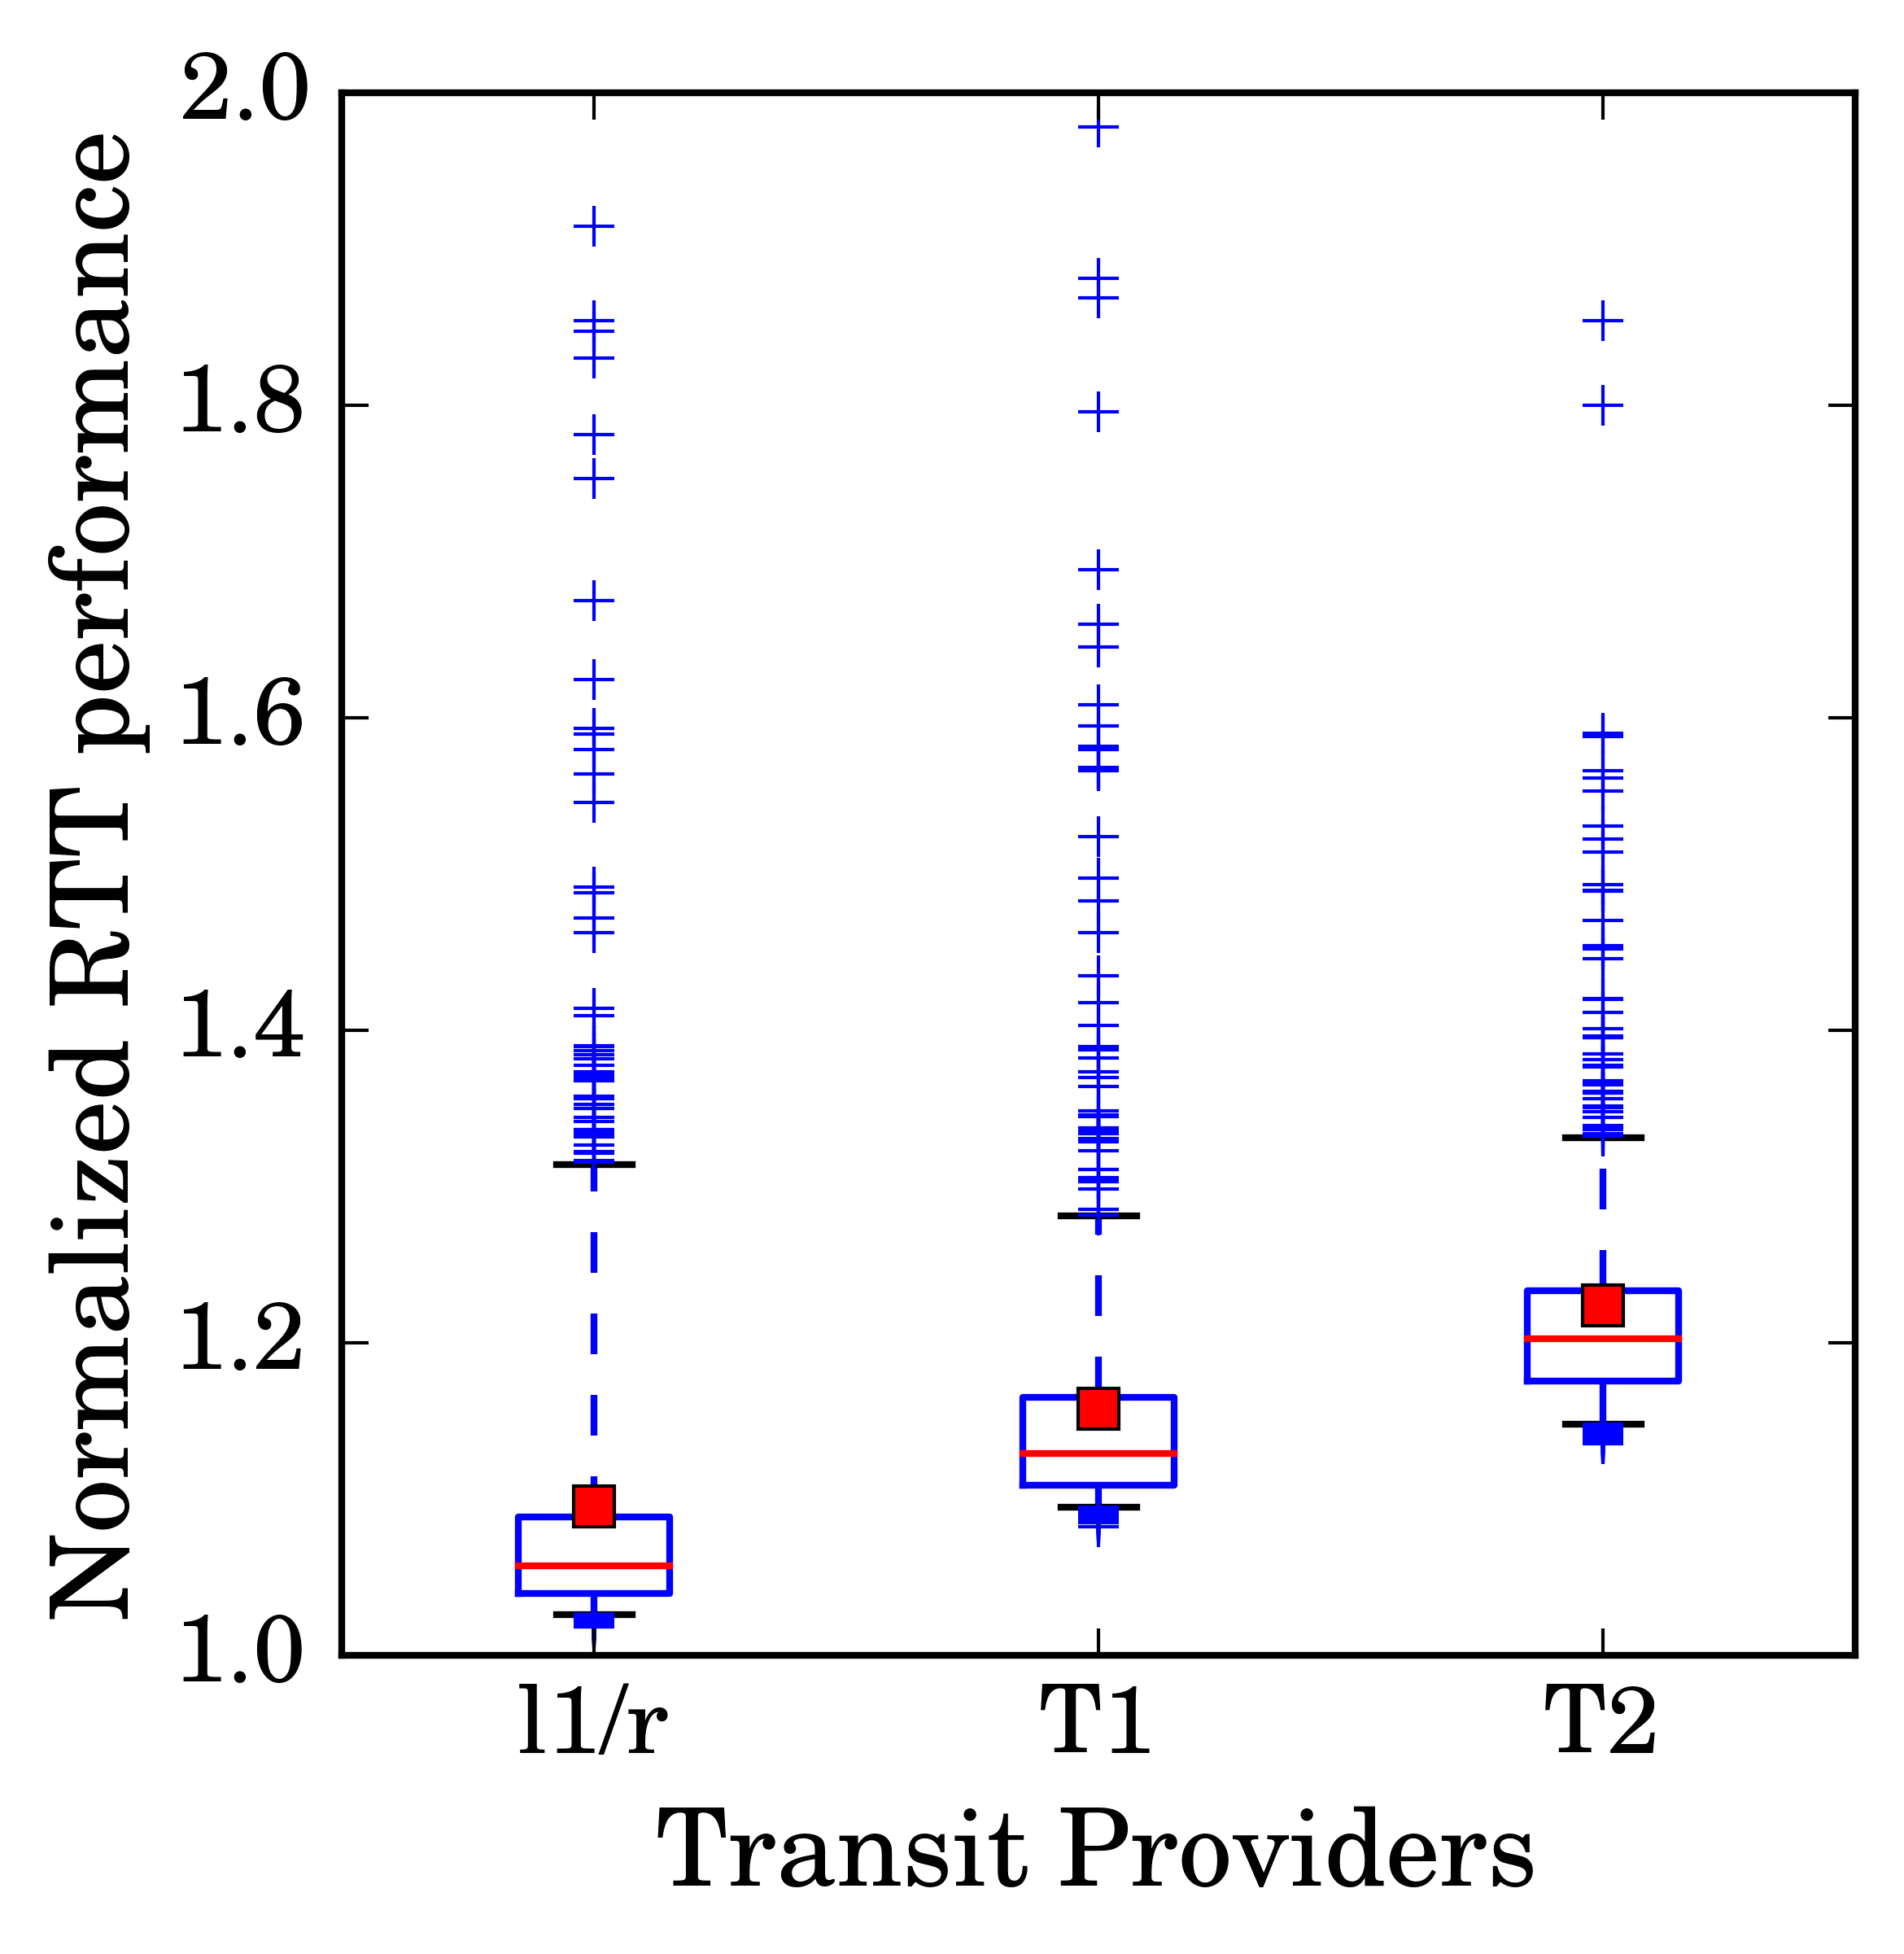
\includegraphics[width=\textwidth]{gfx/chap2/np_box_sf.png}
                \caption{SF, 879 prefixes, $78.49\%$ traffic}
                \label{fig:np_sf}
        \end{subfigure}
\caption{Normalized RTT performance with active probing. Average number of prefixes probed and average traffic volume fraction represented by these prefixes each hour are given.}
\label{fig:np}
\end{figure}
\begin{figure}\ContinuedFloat
	\centering
        \begin{subfigure}[b]{0.48\textwidth}
                \includegraphics[width=\textwidth]{gfx/chap2/np_box_sg.png}
                \caption{SG, 924 prefixes, $63.08\%$ traffic}
                \label{fig:np_sg}
        \end{subfigure}
        \begin{subfigure}[b]{0.48\textwidth}
                \includegraphics[width=\textwidth]{gfx/chap2/np_box_sh.png}
                \caption{SH, 73 prefixes, $2.83\%$ traffic}
                \label{fig:np_sh}
        \end{subfigure}
        \begin{subfigure}[b]{0.48\textwidth}
                \includegraphics[width=\textwidth]{gfx/chap2/np_box_si.png}
                \caption{SI, 642 prefixes, $67.51\%$ traffic}
                \label{fig:np_si}
        \end{subfigure}
\caption{(cont.) Normalized RTT performance with active probing. Average number of prefixes probed and average traffic volume fraction represented by these prefixes each hour are given.}
\label{fig:np_cont}
\end{figure}

In this section, we explore the potential performance gain that client networks can potentially achieve with measurement-based TE.

%\marginpar{how RTT is measured}
In order to evaluate the performance gain, we continuously measured the \acf{RTT} towards selected prefixes (using $MV$ metric with $L=168$) via all available transit providers using TCP SYN scan~\cite{nmap} over the week starting from June 1st, 2015, i.e. the second week of our observation.
The probe traffic is steered by means of explicit routing.
For a pair of selected destination prefix and available transit provider, a probe is scheduled at 240 second interval in average with $30\%$ randomization w.r.t. the interval in timing. 

%\marginpar{how to evaluate transit performance over selected prefixes}
We quantify the performance level of a transit provider with a metric proposed by Akella et al.\ \cite{Akella2003a}. 
This metric first normalizes the RTT via the chosen transit over the smallest RTT  measurement across all available transit providers at the same probe round. This is done for each individual selected prefix.
It then averages this normalized RTT over the entire selected prefix set.
More formally the evaluation is done as the following:
\begin{align*}
NP^{Tx}_{t_i} = \frac{1}{|SP|} \sum_{P \in SP} M^{Tx}_{t_i}(P)/\min_{T_j \in T}M^{T_j}_{t_i}(P)
\label{eq:np}
\end{align*}
where $NP^{Tx}_{t_i}$ is the normalized RTT performance for transit provider $Tx$ at probe round $t_i$, and 
$M^{Tx}_{t_i}(P)$ denotes the RTT measured toward selected prefix $P$ via $Tx$.
If a transit provider offers the smallest RTT to all selected prefixes, it should have a normalized RTT performance equaling to 1. 
On the other hand, a large $NP$ value indicates that the overall transmission performance using that transit provider is far from ideal.

%\marginpar{dynamic route selection as a virtual transit provider}
If the egress transit provider for real traffic is chosen dynamically for each individual destination prefix, the route selection mechanism can be regarded as a virtual transit provider. 
At each probe round, the virtual transit provider corresponds to a set of physical transit provider for each destination prefix. 
The set of physical provides taht are actually employed can change over time, i.e. dynamic.

We implemented a virtual transit provider, denoted as $l1/r$, first appeared in~\cite{Akella2008} for the sake of comparison. 
$l1/r$ selects the transit provider that provides the smallest RTT in last probe round for each destination prefix ($l1$ in $l1/r$). 
When RTT measurement data is not available (e.g. prefix newly selected, measurement timeout), it chooses randomly ($r$ in $l1/r$). 
This choice is based on the hypothesis that RTT of a path demonstrates temporal locality and thus is closely related to its most recent measurement.

Figure~\ref{fig:np} gives the results of transit performance evaluation in a box-plot.
The box stands for $25^{th}$ and $75^{th}$ percentiles. 
The red line tells the medium value, while the red square indicates the mean.
Finally, the whiskers represent $5^{th}$ and $95^{th}$ percentiles (values below and beyond, marked by a \texttt{+} symbol, can be regarded as outliers).
Along the X-axis, available transit providers are aligned from left to right increasingly according to their mean normalized RTT performance (marked by a red square). 

We observe that the performance differences among different transit providers is particularly evident on SC.
This confirms that multi-homing can still provide significant performance improvement nowadays. 
However this gain in performance is not inherently given in the context of BGP, as it it is performance agnostic in route decision.
Even for transit provider that offers the best best mean $NP$, there exist moments where its performance deviates far above 1, which means that traffic toward some selected prefixes are suffering from RTTs much larger than other available transit providers.
This implies that a network can not arrive at optimal performance by using a single transit providers in a static and indistinguishable manner for all the destination prefixes.

For all networks except SG, the virtual transit provider outperforms all physical transit providers.
On SB, the performance metric $NP$ of $l1/r$ is $20\%$ lower than that of the best available transit provider.
Still, the $NP$ value of this virtual provider varies within a wide range, which calls for further investigation into the characters of RTT variation in time, see Section~\ref{sec:ripe_atlas} and \ref{sec:cpt_rtt}.

Finally, we missed RTT measurement for quite a few selected destination prefixes on some client networks, especially SH, SC, SD and SE. Reasons for such massive lack of measurement are explained in Section~\ref{sec:infer}.
A possible solution is given to allow TE for those prefixes without measurements.

\section*{Conclusion}
\label{sec:fut}
This chapter tackled the problem of controlling a majority of data traffic via 
a small subset of BGP prefixes, by exploiting the uneven Internet traffic distribution. 
One of the challenges in addressing this problem was to select in a scalable manner the prefixes that will carry most traffic volume in the forthcoming time.  

%GgX: IMO We talk about a property of traffic, hence "volume" has to be singular.
We analyzed real traffic measurements from nine different networks located in five different countries to understand the distribution of traffic volume associated with BGP prefixes, as well as its variation in time.   
We observed that the most important prefixes (representing largest volume over a week) are generally stable in time, with small hourly variations around their mean of hour volume. 
Based on this observation, we proposed three simple 
%and resource-economical   % GgX: How can a metric demand ressources? Its computation does but not the metric tiself 
metrics (also easy to compute) to proactively select prefixes with important foreseeable traffic volume.
We demonstrated that the metrics we proposed lead to better volume coverage compared to the existing solutions.
Furthermore, we evaluated the transmission performance for selected destination prefixes using multiple transit providers. 
We simulated as well a dynamic route decision algorithm. 
The results showed that with even a fairly basic mechanism, the overall RTT performance could be improved by $20\%$ compared to the best available transit provider in some networks studied. 

\iffalse
We showcased as well that the amount of traffic represented by selected prefixes is reversely correlated to the burstiness of traffic observed on the client networks. How to anticipate the activity of those bursty destination prefixes is then essential to further improve the volume coverage of proposed prefix selection methods.

Understanding the nature of these bursty traffic would greatly help. However, such observation could be related to the business model of each network and thus very difficult to generalize. A possible approach would be introducing a communication channel between the applications generating these bursty traffic and the TE system residing on network layer. In this way, the TE system could be informed in real-time or even in advance of the arrival of large amount of traffic and then intentionally optimize the routing for it.

If the traffic is unintended by the network or untraceable, e.g. in the case of \ac{HP} or public cloud where traffic comes from various entities, the above presented mechanism becomes inapplicable. It is then desired to first detect the presence of these bursty traffic and record its information over long term so that researchers can explore its activity patterns to figure out some sign of predictivity.
\fi

In order to further improve prefix selection methods, we have shown that capturing bursty prefixes is the key. 
To this end, we could group prefixes by their activity profiles. 
For each group, selection method is adapted to its traffic dynamism.
When dealing with prefixes with regular volume patterns and small hourly variation, the simple metrics proposed in this work perform already sufficiently well. 
Nevertheless, for bursty prefixes, we might need a more sophisticate model that extracts additional activity features, for instance long term periodicity.
The burstiness index $\beta$ proposed in this chapter, shown to be very expressive, could be potentially used in prefix characterization and classification and thus is worthy of future work.